\documentclass[11pt]{article}

\usepackage[margin=1in]{geometry}
\usepackage[T1]{fontenc}
\usepackage[utf8]{inputenc}
\usepackage{lmodern}
\usepackage{microtype}
\usepackage{amsmath,amssymb,amsthm,mathtools}
\usepackage{booktabs}
\usepackage{enumitem}
\usepackage[dvipsnames]{xcolor}
\usepackage{tikz}
\usetikzlibrary{arrows.meta,positioning,calc,backgrounds,fit,decorations.pathreplacing}
\usepackage[colorlinks=true,linkcolor=MidnightBlue,citecolor=MidnightBlue,urlcolor=MidnightBlue]{hyperref}

\newtheorem{theorem}{Theorem}[section]
\newtheorem{lemma}[theorem]{Lemma}
\newtheorem{proposition}[theorem]{Proposition}
\theoremstyle{definition}
\newtheorem{definition}[theorem]{Definition}
\newtheorem*{definition*}{Definition}
\theoremstyle{remark}
\newtheorem{remark}[theorem]{Remark}

\newcommand{\todo}[1]{{\color{red}\textbf{[TODO:} #1\textbf{]}}}
\newcommand{\LS}{\mathrm{LS}}
\newcommand{\RS}{\mathrm{RS}}
\newcommand{\LCA}{\mathrm{LCA}}
\newcommand{\Rot}{\mathrm{Rot}}
\newcommand{\ld}{\mathrm{ld}}
\newcommand{\sep}{\mathrm{sep}}
\newcommand{\PUSH}{\textnormal{\scshape Push}}
\newcommand{\POP}{\textnormal{\scshape Pop}}
\newcommand{\INJECT}{\textnormal{\scshape Inject}}
\newcommand{\EJECT}{\textnormal{\scshape Eject}}
\newcommand{\SHIFT}{\textnormal{\scshape Shift}}
\newcommand{\UPROT}{\textnormal{\scshape UpperRot}}
\newcommand{\BuildScaleTree}{\textnormal{\scshape BuildScaleTree}}

\title{\textbf{Breaking All Iterated Inverse-Ackermann Bounds\\for the Deque Conjecture on Splay Trees}}
\author{
  Goran \v{Z}u\v{z}i\'{c}\\[-2pt]
  {\small Google Research}
  \and
  Sorrachai Yingchareonthawornchai\\[-2pt]
  {\small ETH Zurich}
  \and
  David P. Woodruff\\[-2pt]
  {\small Google Research \& CMU}
  \and
  Vahab Mirrokni\\[-2pt]
  {\small Google Research}
}
\date{November 2026}

\begin{document}
\maketitle
\pagenumbering{roman}
\begin{abstract}
Tarjan's Deque Conjecture (1985) asserts that executing any sequence of $m$ double-ended queue operations (\PUSH, \POP, \INJECT, \EJECT) on an $n$-node splay tree performs $O(m + n)$ rotations. Prior upper bounds progressed from $O\big((m + n)\log(m + n)\big)$ (Sleator and Tarjan, 1985) to $O\big((m + n)\,\alpha(m + n)\big)$ (Sundar, 1992) and $O\big((m + n)\,\alpha^*(m + n)\big)$ (Pettie, 2008), where $\alpha$ is the inverse Ackermann function and $\alpha^*(N)$ is the number of applications of $\alpha$ from $N$ to a constant.  

We prove a new upper bound of $O\big((m + n)\,\alpha_\omega(m + n)\big)$, where $\alpha_\omega(N)$ is the number of stars required on the inverse Ackermann function before its value at \(N\) falls below a fixed threshold, and $\alpha_\omega(N) = o\big(\alpha^{**\ldots*}(N)\big)$ for any fixed number of stars, breaking Pettie's $\alpha^*$ bound.
To our knowledge, this extraordinarily slowly growing function, discussed as a theoretical illustration in (Erickson, 2013), appears for the first time in a bound for a natural algorithmic problem.

We develop a scale-tree method for deriving amortized recurrences by jointly accounting for rotation costs across multiple levels of a hierarchical block decomposition. Our method extends Sundar's classical cascade counting and builds on Pettie's approach to controlling interactions between recursive subproblems.

Our proof is self-contained, holds unconditionally for all $m, n \ge 0$, and is formally verified in Lean~4 together with every intermediate proposition, lemma, and reduction in the paper (\href{https://github.com/sorrachai/SplayTree-Deque-Ordinal-Inverse-Ackermann-Bound}{\texttt{github.com/\allowbreak sorrachai/\allowbreak SplayTree-\allowbreak Deque-\allowbreak Ordinal-\allowbreak Inverse-\allowbreak Ackermann-\allowbreak Bound}}).
\end{abstract}
\newpage
\tableofcontents
\newpage
\pagenumbering{arabic}

% ============================================================================
\section{Introduction}
\label{sec:intro}
% ============================================================================

\subsection{Splay Trees and Tarjan's Deque Conjecture}

Sleator and Tarjan~\cite{SleatorTarjan1985} introduced \emph{splay trees}, self-adjusting binary search trees (BSTs) that maintain no balance metadata and restructure solely by moving each accessed key to the root via bottom-up double rotations (\emph{splaying}). They proved that splay trees match the $O(\log n)$ amortized bound of balanced search trees and posed the \emph{Dynamic Optimality Conjecture}, asserting that splay trees are $O(1)$-competitive with every dynamic BST algorithm on every access sequence. The current best known competitiveness for splay trees~\cite{Splay2026} is $\tilde O(\log\log n)$.  

Several landmark special cases of dynamic optimality have been established on splay trees, including the \emph{Sequential Access Theorem}~\cite{Tarjan1985,Elmasry2004}, the \emph{Dynamic Finger Theorem}~\cite{ColeMishraSchmidtSiegel2000,Cole2000}, and splaying preorders and postorders from an empty tree~\cite{LevyTarjan2019}. Alongside sequential access, Tarjan~\cite{Tarjan1985} posed the \emph{Deque Conjecture}: when a splay tree maintains a double-ended queue supporting insertions and deletions at both ends of the key order, any sequence of $m$ operations starting from an $n$-node BST performs $O(m + n)$ single rotations. Tarjan~\cite{Tarjan1985} and Elmasry~\cite{Elmasry2004} proved this $O(m + n)$ bound for \emph{output-restricted} splay deques (where deletions occur at only one end), whereas the general two-sided case has remained open. On other dynamic BST algorithms, Multi-Splay trees~\cite{WangDerryberrySleator2006} (building on Tango trees~\cite{DemaineHarmonIaconoPatrascu2007}) achieve $O(1)$ amortized cost per deque operation starting from an empty tree~\cite{DerryberrySleatorWang2009}, and geometric forbidden-matrix analyses of Greedy BSTs~\cite{DemaineHarmonIaconoKanePatrascu2009} (cf.~\cite{ChalermsookGoswamiKozmaMehlhornSaranurak2015FOCS} for static pattern-avoiding accesses) achieve $O(m + n)$ for output-restricted deques~\cite{ChalermsookGoswamiKozmaMehlhornSaranurak2015WADS} and $O\big((m + n)\,\alpha(m + n)\big)$ for general two-sided deques~\cite{Chalermsook2023}.

To state the problem precisely, let $T$ be a rooted BST storing distinct real keys in symmetric (in-order) order, so every key in the left subtree of a vertex $u$ is smaller than $u$ and every key in its right subtree is larger than $u$. The \emph{left spine} $\LS(T)$ and \emph{right spine} $\RS(T)$ are the paths obtained by starting at the root of $T$ and repeatedly following left-child or right-child pointers, respectively. A \emph{single rotation} $[x, p]$ promotes a child $x$ one step above its parent $p$ while preserving symmetric key order (a \emph{right rotation} when $x$ is the left child of $p$, i.e., $x < p$, and a \emph{left rotation} when $x > p$). Bottom-up $\mathrm{Splay}(x)$ moves a target vertex $x \in V(T)$ to the root two levels at a time by repeatedly applying:
\begin{itemize}[leftmargin=2em, itemsep=1pt]
  \item \emph{zig} ($1$ single rotation): if $x$'s parent $p$ is the root, rotate $[x, p]$;
  \item \emph{zig-zig} ($2$ single rotations): if $x$ and its parent $p$ are both left children (or both right children) of grandparent $g$, rotate $[p, g]$ first and then $[x, p]$;
  \item \emph{zig-zag} ($2$ single rotations): if one of $x, p$ is a left child and the other is a right child of $g$, rotate $[x, p]$ first and then $[x, g]$.
\end{itemize}
To use a splay tree $T$ as a double-ended queue supporting insertions and deletions at the minimum (left) and maximum (right) ends of the current key set, the four standard splay-tree deque operations~\cite{Tarjan1985,Sundar1992,Pettie2008} are:
\begin{itemize}[leftmargin=2em, itemsep=1pt]
  \item $\PUSH$: insert a new key strictly smaller than $\min V(T)$ directly as the new root, with empty left subtree and the old tree $T_{\mathrm{old}}$ as its right subtree ($0$ rotations).
  \item $\INJECT$: insert a new key strictly larger than $\max V(T)$ directly as the new root, with $T_{\mathrm{old}}$ as its left subtree and empty right subtree ($0$ rotations).
  \item $\POP$ (when $T \ne \emptyset$): splay the minimum key $x_{\min} = \min V(T)$ to the root (which performs $|\LS(T)| - 1$ single rotations up $\LS(T)$) and delete $x_{\min}$, leaving its right subtree $\mathrm{right}(x_{\min})$.
  \item $\EJECT$ (when $T \ne \emptyset$): splay the maximum key $x_{\max} = \max V(T)$ to the root (which performs $|\RS(T)| - 1$ single rotations up $\RS(T)$) and delete $x_{\max}$, leaving its left subtree $\mathrm{left}(x_{\max})$.
\end{itemize}
Write $\Rot(T_0, S)$ for the total number of single rotations performed across a valid $m$-operation sequence $S$ starting from an $n$-node BST $T_0$. Over four decades, upper bounds on $\Rot(T_0, S)$ have climbed a sequence of functional inverses of the Ackermann hierarchy:
\begin{itemize}[leftmargin=2em]
  \item \textbf{Sleator and Tarjan~\cite{SleatorTarjan1985} (1985):} $O\big((m + n)\log(m + n)\big)$ via the access lemma.
  \item \textbf{Sundar~\cite{Sundar1992} (1992):} $O\big((m + n)\,\alpha(m + n)\big)$, reducing deque sequences via path-halving and cascade simplifications (building on~\cite{TarjanVanLeeuwen1984,Tarjan1985,Lucas1990,Lucas1992}; see also~\cite{BuchsbaumSundarTarjan1995}) to block decompositions and an inverse-Ackermann analysis of $0$-gapped right $(2i)$-cascades.
  \item \textbf{Pettie~\cite{Pettie2008} (2008):} $O\big((m + n)\,\alpha^*(m + n)\big)$, reducing two-sided deques via spinal path-compression systems to $\{a b a a b b a,\, a b a b a b a\}$-free sequences, bounded via order-$5$ Davenport--Schinzel sequences~\cite{HartSharir1986,Sharir1987,AgarwalSharirShor1989} (see also~\cite{SeidelSharir2005,Nivasch2010,Pettie2010} for related path-compression, generalized Davenport--Schinzel, and forbidden $0$--$1$ matrix bounds).
\end{itemize}

\subsection{Main Result: Breaking All Finite Star-Iterates}

To fix concrete thresholds without base-case ambiguity, we follow Sundar's indexing of the Ackermann hierarchy~\cite[Section~1.2]{Sundar1992}. Each function in the hierarchy below inverts or iterates the previous one, producing progressively slower-growing functions of $n$.

\begin{definition}[Ackermann Hierarchy, Finite Star-Iterates $\alpha_r$, and Level-$\omega$ Star-Iterate $\alpha_\omega$]
\label{def:ackermann}
We define the fast-growing Ackermann table $A_i(j)$ and its functional inverses in four steps:
\begin{enumerate}[label=(\arabic*), leftmargin=2em, itemsep=2pt]
  \item \emph{Ackermann table $A_i(j)$.} Each row $A_i : \mathbb{Z}_{\ge 1} \to \mathbb{Z}_{\ge 1}$ ($i \ge 0$) repeatedly composes the previous row, escalating from doubling to exponentiation, power towers, and beyond: set $A_0(j) := 2j$, $A_1(j) := 2^j$, and for $i \ge 2$,
  \[
  A_i(1) \;:=\; A_{i-1}(2), \qquad A_i(j) \;:=\; A_{i-1}\big(A_i(j - 1)\big) \quad (j \ge 2).
  \]
  (For example, $A_2(j)$ is a tower of $j + 1$ twos, giving $A_1(1) = 2$, $A_2(1) = 4$, $A_3(1) = 16$, and $A_4(1) = A_2(16) > 2^{65536}$.)
  \item \emph{Inverse Ackermann function $\alpha_0(n)$.} For $n \ge 1$, $\alpha_0(n)$ is the first row whose initial entry $A_k(1)$ reaches $n$ (written $\bar{\alpha}(n)$ in Sundar~\cite{Sundar1992}):
  \[
  \alpha_0(n) \;:=\; \min\big\{k \ge 1 : A_k(1) \ge n\big\}.
  \]
  \item \emph{Star operator $f^*$ and finite star-iterates $\alpha_r(n)$.} Given any function $f : \mathbb{Z}_{\ge 1} \to \mathbb{Z}_{\ge 1}$ satisfying $f(n) < n$ for all $n > 4$, its \emph{star-iterate} $f^* : \mathbb{Z}_{\ge 1} \to \mathbb{Z}_{\ge 1}$ counts ($1$ plus) how many times $f$ must be applied to reduce $n$ to at most~$4$: $f^*(n) := 1$ for $n \le 4$, and $f^*(n) := 1 + f^*(f(n))$ for $n > 4$. Applying $(\cdot)^*$ repeatedly starting from $\alpha_0$ defines the $r$-th star-iterated inverse Ackermann function $\alpha_r := (\alpha_{r-1})^* : \mathbb{Z}_{\ge 1} \to \mathbb{Z}_{\ge 1}$ for each integer $r \ge 1$:
  \begin{equation}
  \label{eq:alpha-r}
  \alpha_r(n) \;:=\;
  \begin{cases}
  1 & \text{if } n \le 4,\\
  1 + \alpha_r\big(\alpha_{r-1}(n)\big) & \text{if } n > 4,
  \end{cases}
  \end{equation}
  so $\alpha_1 = \alpha^*$, $\alpha_2 = (\alpha^*)^* = \alpha^{**}$, and $\alpha_3 = ((\alpha^*)^*)^* = \alpha^{***}$.
  \item \emph{Level-$\omega$ star-iterate $\alpha_\omega(n)$.} Rather than fixing the number of stars $r$ in advance, $\alpha_\omega(n)$ counts how many stars must be placed on $\alpha_0$ before the value at $n$ drops to at most~$2$:
  \[
  \alpha_\omega(n) \;:=\; \min\big\{r \ge 1 : \alpha_r(n) \le 2\big\}.
  \]
\end{enumerate}
\end{definition}

\begin{remark}[Notation and Why We Write $\alpha_\omega$]
\label{rem:lob-wainer}
Two conventions are worth noting. First, in $\alpha_0, \alpha_1, \alpha_2, \dots$, the subscript counts how many times the star operator $(\cdot)^*$ is applied to $\alpha_0$ (so $\alpha_1 = \alpha^*$ and $\alpha_2 = (\alpha^*)^* = \alpha^{**}$), rather than indexing row inverses of the Ackermann table $A_k(\cdot)$ as in the Davenport--Schinzel literature~\cite{AgarwalSharirShor1989,Nivasch2010}. Second, just as $\alpha_0(n)$ diagonalizes across the finite rows $A_1, A_2, \dots$, the function $\alpha_\omega(n) = \min\{r \ge 1 : \alpha_r(n) \le 2\}$ diagonalizes across the infinite sequence of star-iterates $\alpha_1, \alpha_2, \dots$ (this diagonalized star-counting function also appears as an illustrative theoretical construct in Erickson~\cite[Section~11.7]{Erickson2013}; in logic's fast-growing hierarchy~\cite{LobWainer1970I,LobWainer1970II}, $\alpha_0$, $\alpha_r$, and $\alpha_\omega$ correspond to levels $\omega$, $\omega + r$, and $\omega \cdot 2$; see Proposition~\ref{prop:lob-wainer} in Appendix~\ref{app:ackermann}).
\end{remark}

The function $\alpha_\omega(n)$ grows strictly slower than every finite star-iterate $\alpha_r(n)$, and does not depend (up to an additive constant) on whether we invert $A_k(1)$ or the diagonal Ackermann function $A_k(k)$ (proofs of routine Ackermann estimates are deferred to Appendix~\ref{app:ackermann}):

\begin{proposition}[Asymptotic Dominance and Convention Invariance]
\label{prop:omega-properties}
The function $\alpha_\omega$ is non-decreasing with $\alpha_\omega(n) = 1$ for all $1 \le n \le A_4(1) = A_2(16) > 2^{65536}$, $\lim_{n \to \infty} \alpha_\omega(n) = \infty$, and for every fixed integer $r \ge 1$,
\[
\alpha_\omega(n) \;<\; \log_2 \alpha_r(n) \quad \text{for all sufficiently large } n,
\qquad\text{hence}\qquad
\alpha_\omega(n) \;=\; o\big(\alpha_r(n)\big) \quad (n \to \infty).
\]
Moreover, if we instead invert the diagonal Ackermann function via $\widetilde{\alpha}_0(n) := \min\{k \ge 1 : A_k(k) \ge n\}$, define its star-iterates $\widetilde{\alpha}_r$ ($r \ge 1$) by the recursion~\eqref{eq:alpha-r}, and diagonalize via $\widetilde{\alpha}_{\omega,\mathrm{diag}}(n) := \min\{r \ge 1 : \widetilde{\alpha}_r(n) \le r\}$, then $\widetilde{\alpha}_{\omega,\mathrm{diag}}(n) - 1 \le \alpha_\omega(n) \le \widetilde{\alpha}_{\omega,\mathrm{diag}}(n) + 2$ for every $n \ge 1$.
\end{proposition}

Our main theorem breaks Pettie's $\alpha^*$ barrier and every finite star-iterated bound $O\big((m + n)\,\alpha_r(m + n)\big)$ simultaneously:

\begin{theorem}[Main Theorem]
\label{thm:main}
There exists an absolute constant $C > 0$ such that for every $n$-node BST $T_0$ ($n \ge 0$) and every valid sequence $S$ of $m \ge 0$ splay-tree deque operations ($\PUSH$, $\POP$, $\INJECT$, $\EJECT$) containing $d_L$ $\POP$ deletions and $d_R$ $\EJECT$ deletions ($d := d_L + d_R$),
\begin{align*}
\Rot(T_0, S)
&\;\le\; C\Big(n + m + d_L\,\alpha_\omega\big(\max(d_L, 1)\big) + d_R\,\alpha_\omega\big(\max(d_R, 1)\big)\Big)\\
&\;=\; O\!\Big((m + n)\,\alpha_\omega\big(\max(m + n, 1)\big)\Big).
\end{align*}
\end{theorem}

Because Theorem~\ref{thm:main} is parameterized by the deletion counts $d_L, d_R$ rather than $m + n$ alone, any execution performing $d = O\big((m + n)/\alpha_\omega(\max(m + n, 1))\big)$ deletions already performs $O(m + n)$ rotations; and because the same universal bound holds for all $m, n \ge 0$ without a separate base-case threshold, $\alpha_\omega\big(\max(m + n, 1)\big) = 1$ gives $\Rot(T_0, S) \le 2C(m + n)$ for all $m + n \le A_2(16)$.

\paragraph{Formal verification in Lean~4.}
Theorem~\ref{thm:main} and every numbered proposition, lemma, and theorem in Sections~\ref{sec:intro}--\ref{sec:frontiers} and Appendix~\ref{app:ackermann} have been formalized and mechanically verified in Lean~4 (\texttt{v4.35.0}) \cite{MouraUllrich2021} on top of \texttt{AlgoLib}'s BST and bottom-up splay-tree library \cite{AlgoLib2026} (\texttt{AlgoLib.\allowbreak DataStructures.\allowbreak SplayTree.\allowbreak Complexity}), using the exact definitions and threshold conventions of Definitions~\ref{def:ackermann} and~\ref{def:scale-tree}; the complete repository (including the paper and all Lean~4 source files) is available at \href{https://github.com/sorrachai/SplayTree-Deque-Ordinal-Inverse-Ackermann-Bound}{\texttt{https://github.com/\allowbreak sorrachai/\allowbreak SplayTree-\allowbreak Deque-\allowbreak Ordinal-\allowbreak Inverse-\allowbreak Ackermann-\allowbreak Bound}}. It separates a minimal specification of the main result in \href{https://github.com/sorrachai/SplayTree-Deque-Ordinal-Inverse-Ackermann-Bound/blob/main/ChallengeMain.lean}{\texttt{ChallengeMain.lean}} from a full blueprint of all $28$ intermediate reductions and helper lemmas in \href{https://github.com/sorrachai/SplayTree-Deque-Ordinal-Inverse-Ackermann-Bound/blob/main/ChallengeHelpers.lean}{\texttt{ChallengeHelpers.lean}}; the proof modules \href{https://github.com/sorrachai/SplayTree-Deque-Ordinal-Inverse-Ackermann-Bound/blob/main/SolutionMain.lean}{\texttt{SolutionMain.lean}} and \href{https://github.com/sorrachai/SplayTree-Deque-Ordinal-Inverse-Ackermann-Bound/blob/main/SolutionHelpers.lean}{\texttt{SolutionHelpers.lean}} compile without \texttt{sorry}, use only Lean's standard classical axioms (\texttt{propext}, \texttt{Classical.\allowbreak choice}, \texttt{Quot.sound}), and pass Lean's external kernel check against both specifications via \texttt{lake comparator}.

\subsection{Overview of Techniques and Comparison with Prior Work}
\label{subsec:techniques}

Why did prior upper bounds on splay-tree deques stop at $\alpha_0(m + n)$~\cite{Sundar1992} and $\alpha_1(m + n) = \alpha^*(m + n)$~\cite{Pettie2008}, and how does our analysis reach $\alpha_\omega(m + n)$? We first compare our approach directly with the methods of Sundar~\cite{Sundar1992} and Pettie~\cite{Pettie2008} and summarize our main new ingredients (Section~\ref{subsubsec:prior-and-novelty}); we then walk step by step through each module of our proof (Sections~\ref{subsubsec:step12}--\ref{subsubsec:step45}), defining every technical concept before using it, separating each mathematical claim from its consequences, and linking every step to the exact theorems and lemmas proved later in the paper.

\subsubsection{Comparison with Sundar (1992) and Pettie (2008), and Overview of Novelty}
\label{subsubsec:prior-and-novelty}

Both Sundar~\cite{Sundar1992} and Pettie~\cite{Pettie2008} follow a two-stage strategy: first reduce a general two-sided deque execution ($\PUSH, \POP, \INJECT, \EJECT$) to a one-sided problem where keys are deleted from only one end, and then partition the keys into contiguous blocks to bound long chains of rotations across block boundaries. They differ sharply in how they control cross-block rotations and whether they recurse into smaller subproblems.

\paragraph{Sundar's static cascade method ($O\big((m + n)\,\alpha_0(m + n)\big)$~\cite{Sundar1992}).}
To eliminate two-sided deletions, Sundar divides the operation sequence into \emph{operation-count epochs}: starting from a $k$-node BST, an epoch consists of the next $\max(\lfloor k/2 \rfloor, 1)$ operations of any type, ensuring that neither the $\lceil k/2 \rceil$ smallest keys nor the $\lfloor k/2 \rfloor$ largest keys initially present can empty during the epoch so the left and right halves can be analyzed separately~\cite[Section~3, Theorem~7]{Sundar1992}. Within the left half, Sundar pre-attaches each future $\PUSH$ key as the symmetric-order successor of the last key popped before it (simulating $\PUSH$ by right-rotating it to the root), folds the right spine upside-down onto the left spine, and right-rotates popped keys onto the folded right spine instead of deleting them, embedding the epoch into a single static $N$-node BST evolving solely by right single rotations~\cite[Section~3, Lemma~10]{Sundar1992}. Call any path following only left-child pointers a \emph{left-child path}, and define a \emph{$0$-gapped right $k$-cascade} on a pure-right-rotation BST to be a batch of $k$ simultaneous, vertex-disjoint right single rotations $[x_1, y_1], \dots, [x_k, y_k]$ occurring consecutively (with zero unrotated vertices between pairs) along a single left-child path.
\begin{itemize}[leftmargin=2em, itemsep=2pt]
  \item \emph{Sundar's core claim~\cite[Section~2.1, Theorem~3]{Sundar1992}:} For every integer $i \ge 1$ and every $N \le A_i(1)$, any pure-right-rotation sequence on an $N$-node BST executes at most $O(N)$ $0$-gapped right $(2i)$-cascades (proved by partitioning the $N$ keys into contiguous blocks and maintaining a summary tree retaining at most $2$ top vertices per block to induct from $2(i - 1)$ to $2i$; cf.~Sundar's Scanning Theorem generalization~\cite[Section~4.2, Theorem~8]{Sundar1992}, which retains $4d$ preorder vertices per block to bound $d$-shallow twists).
  \item \emph{Consequence and bottleneck at $\alpha_0$~\cite[Section~3, Lemma~9]{Sundar1992}:} On a one-sided epoch of $P$ keys, setting $i := \alpha_0(P)$ ensures $P \le A_i(1)$, so splitting each $k$-rotation $\POP$ into $\lfloor k / (2i) \rfloor$ disjoint $0$-gapped right $(2i)$-cascades bounds the number of full $(2i)$-cascades across the epoch by $O(P)$. However, because Sundar applies Theorem~3 directly to the uncontracted $P$-node BST rather than contracting blocks of size $\Theta(i^2)$ into a summary tree of $P / \Theta(i^2)$ nodes and recursing inside blocks, \emph{both} the $O(P)$ full $(2i)$-cascades ($2i$ rotations each) \emph{and} the up to $2i - 1$ leftover rotations per $\POP$ contribute $O(i P) = O\big(P\,\alpha_0(P)\big)$ single rotations, stopping the bound at $O\big((m + n)\,\alpha_0(m + n)\big)$.
\end{itemize}

\paragraph{Pettie's sequential Davenport--Schinzel recursion ($O\big((m + n)\,\alpha^*(m + n)\big)$~\cite{Pettie2008}).}
Pettie splits the execution into \emph{size-halving phases}---contiguous intervals ending once half of the active keys present at the start of the phase have been deleted---and applies \emph{spine folding}~\cite[Section~2, Observation~2.1 and Figure~2]{Pettie2008}: flipping the right spine of the left-half BST upside-down onto the top of its left spine merges both spines into a single path. Under Knuth's classical first-child/right-sibling bijection between binary trees and ordered trees~\cite[Section~2.3.2]{Knuth1997Vol1} (where a vertex's left child in the binary tree becomes its leftmost child in the ordered tree, and its right child becomes its right sibling), paired right rotations along the BST left spine become \emph{halving spinal path compressions}---operations that reassign every second vertex along a subpath of the ordered tree's leftmost spine to its grandparent. To bound cross-block compressions, recall that an \emph{order-$5$ Davenport--Schinzel sequence} on $z$ symbols is a sequence with no two equal adjacent symbols and no alternating $7$-symbol subsequence of the form $a b a b a b a$ ($a \ne b$); Agarwal, Sharir, and Shor~\cite{AgarwalSharirShor1989} proved that every such sequence has length at most $z\,\beta(z)$ for a function $\beta(z) = \alpha_0(z)^{O(\alpha_0(z))}$.
\begin{itemize}[leftmargin=2em, itemsep=2pt]
  \item \emph{Pettie's core claim~\cite[Lemmas~4.1--4.4 and Section~5]{Pettie2008}:} Partitioning $P$ keys at a single block size $B := \beta(P)^2$, the cross-block contacts of all spinal path compressions transcribe into a repetition-free sequence on $O(P / B)$ block-period labels (splitting each block's timeline into deletion periods) that avoids both $a b a a b b a$ and $a b a b a b a$ ($a \ne b$). Bounding the spawned cross-block compression systems---which also carry non-essential ``fluff'' spine vertices (deleted at the bottom at linear cost) and ``stunted'' compressions terminating below the root---via the order-$5$ Davenport--Schinzel bound limits their total essential size to $O\big((P/B)\,\beta(P/B)\big) = O\big(P / \beta(P)\big)$ (so recursing on them costs $o(P)$), absorbing all cross-block work into $O(P)$ additive overhead and leaving $P / B$ intra-block deque subproblems of size $B = \beta(P)^2$.
  \item \emph{Consequence and bottleneck at $\alpha^*$:} Unlike Sundar, Pettie recurses on the intra-block subproblems, shrinking the active problem size along
  \[
  P \;\longmapsto\; \beta(P)^2 \;\longmapsto\; \beta\big(\beta(P)^2\big)^2 \;\longmapsto\; \cdots \;\longmapsto\; O(1)
  \]
  (since $\beta(\beta(P)^2)^2 < \alpha_0(P)$ for large $P$, every two recursion steps overtake $\alpha_0$). However, because Pettie's recursion resolves \emph{one block scale $B$ per pass} and pays $O(P)$ cross-block overhead across all blocks at that scale, the $\Theta(\alpha^*(P))$ sequential recursion levels accumulate $O\big(P\,\alpha^*(P)\big)$ in the upper-bound recurrence. Any method that contracts one block scale per pass faces this $\Theta(\alpha^*)$ barrier.
\end{itemize}

\paragraph{Novelty of our method ($O\big((m + n)\,\alpha_\omega(m + n)\big)$).}
Breaking through $\alpha^*$---and through every finite star-iterate $\alpha_r$---requires amortizing across an arbitrarily long hierarchy of nested block scales \emph{simultaneously within a single linear-overhead pass}, without blowing up subproblem parameters or paying per-scale boundary costs. Our proof introduces four technical ingredients (summarized alongside Sundar and Pettie in Table~\ref{tab:comparison} at the end of Section~\ref{subsec:techniques}):
\begin{enumerate}[label=(\arabic*), leftmargin=2em, itemsep=2pt]
  \item \emph{Epoch-free global reduction to a self-similar folded $\POP$ process (Section~\ref{sec:reduction}, Theorem~\ref{thm:mod1-reduction}; Section~\ref{sec:scale-tree}, Lemma~\ref{lem:bucket-leaf}):} Instead of epochs or multi-parameter compression systems with fluff vertices, an offline three-way key partition (Lemma~\ref{lem:nested-keys}) and a joint spine potential (Lemma~\ref{lem:spine-accounting}) reduce the entire two-sided deque execution in \emph{one global step} to two independent one-sided pure-right-rotation processes. Crucially, restricting this one-sided process to any contiguous finest-scale block during its deletion window yields an exact subproblem of the \emph{identical one-parameter form} with zero parameter blowup (Lemma~\ref{lem:bucket-leaf}).
  \item \emph{Linear-in-gap right-cascade bound replacing Davenport--Schinzel sequences (Section~\ref{sec:cascades}, Theorem~\ref{thm:mod2-cascade}):} Rather than transcribing compressions into $\{a b a a b b a, a b a b a b a\}$-free strings (which loses $\beta(z) = \alpha_0(z)^{O(\alpha_0(z))}$), we unify Sundar's Theorem~3 $(2i)$-cascade recursion with his Section~4.2 preorder-$D$ summary tree (at $D = \Delta' + 2$) to allow up to $\Delta'$ unrotated gap vertices between consecutive rotated pairs along a left-child path. We prove that the $(2i)$-cascade count grows \emph{linearly} as $O((\Delta' + 1) N)$ for $N \le A_i(1)$ (avoiding the exponential $(\Delta' + 1)^{2i}$ loss of naive gap pigeonholing), shrinking the required block size from $\beta(P)^2$ down to a quadratic polynomial in $\alpha_0$ with tunable per-scale weights and no Davenport--Schinzel machinery.
  \item \emph{Simultaneous multi-scale amortization and weight resets via scale trees (Sections~\ref{sec:scale-tree}--\ref{sec:contraction}, Definition~\ref{def:scale-tree}, Lemma~\ref{lem:tree-weights}, and Theorem~\ref{thm:mod4-contraction}):} Instead of resolving scales sequentially one pass at a time, we maintain $M$ nested block partitions at once and arrange the scales $\{1, \dots, M\}$ as the leaves of a rooted \emph{scale tree} of height $r$ whose edges to $c$-th children carry quadratic multipliers $4 c^2$, giving each leaf a weight equal to the product of multipliers along its root-to-leaf path. These multipliers keep the reciprocal leaf weights summable to $< \frac{1}{2}$ for \emph{every} height $r$ and \emph{any} $M$, while resetting child counters $c = 1, 2, \dots$ on every fresh subtree so block contraction accelerates from $\alpha^*$ (height~$1$) to $\alpha_r$ (height~$r$).
  \item \emph{Four-way scale routing and a height-independent $O(P)$ bound on three-block rotations (Section~\ref{sec:scale-tree}, Lemmas~\ref{lem:bucket-leaf}--\ref{lem:bucket-b2} and Theorem~\ref{thm:mod3-pass}):} When $M$ scales coexist in one pass, a single deletion can trigger rotations across many scales. We classify every rotation into four classes by comparing the scale separating the deleted key from the promoted key against the scale separating the rotated pair itself. Split-scale rotations (where those two scales differ) route to their lowest common ancestor in the scale tree and step monotonically up or down the tree across consecutive rotations within one $\POP$ step ($\le r$ steps, costing $O(r P)$), while our central technical estimate proves that three-block rotations occurring at a single scale cost $O(P)$ \emph{with zero dependence on $r$ or $M$} (Lemma~\ref{lem:bucket-b3-exit}). Because downward split-scale chains can terminate into three-block rotations, this height-independent $O(P)$ bound prevents an $O(r^2 P)$ blowup and yields $O(r P)$ total pass overhead across all $M$ scales, giving Theorem~\ref{thm:main} at $r = \alpha_\omega(P)$.
\end{enumerate}

\subsubsection{Step 1 \& Step 2: The Folded \texorpdfstring{$\POP$}{Pop} Process and Bounded-Gap Cascades}
\label{subsubsec:step12}

\paragraph{Step 1: Eliminating two-sided operations via the folded $\POP$ process (Section~\ref{sec:reduction}).}
In a general splay-tree deque $(T_0, S)$, $\POP$ splays the minimum key up the left spine $\LS(T)$ via zig-zig steps (and at most one final zig), while $\EJECT$ splays the maximum key up the right spine $\RS(T)$ via symmetric zig-zig steps. Our first step eliminates $\INJECT$, $\EJECT$, never-deleted middle keys, right-spine left rotations, and the bottom-node-carrying second rotation of each zig-zig, isolating a one-sided pure-right-rotation game on $P$ keys deleted in fixed order $1, 2, \dots, P$.

Write $u(A, B)$ for the BST rooted at key $u$ with left subtree $A$ and right subtree $B$. Formally, a \emph{folded $\POP$ process} $\widetilde{H}$ of size $P \ge 1$ (Definition~\ref{def:folded-pop}, illustrated in Figures~\ref{fig:folded-ops} and~\ref{fig:folded-pop}) is a dynamic BST execution on key universe $\{1, \dots, P\}$ starting from $\widetilde{H} = \emptyset$. Whenever the active key set $V \subseteq \{1, \dots, P\}$ is non-empty, the state carries a marked vertex $b_1 \in \LS(\widetilde{H})$, called the \emph{fold boundary}, which splits $\LS(\widetilde{H})$ into the \emph{lower spine} $\{v \in \LS(\widetilde{H}) : v < b_1\}$ and the \emph{upper spine} $\{v \in \LS(\widetilde{H}) : v \ge b_1\}$ (corresponding under spine folding to the left spine and reversed right spine of an unfolded one-sided BST). Across the execution, $\widetilde{H}$ undergoes $P$ $\PUSH$ steps, $P$ $\POP$ steps (deleting $s = 1, 2, \dots, P$ in increasing order), and $K_{\SHIFT}$ $\SHIFT$ steps plus $K_{\mathrm{rot}}$ $\UPROT$ steps subject to the total upper-spine budget $K_{\SHIFT} + K_{\mathrm{rot}} < 2P$:
\begin{itemize}[leftmargin=2em, itemsep=1pt]
  \item $\PUSH(w)$ ($0$ rotations) inserts a new minimum key $w \in \{1, \dots, P\}$ ($w < \min V$ when $V \ne \emptyset$): if $\widetilde{H} = \emptyset$, set $\widetilde{H} \gets w(\emptyset, \emptyset)$ and $b_1 \gets w$; otherwise splice $w$ directly below $b_1$ via $\mathrm{left}_{\widetilde{H}}(b_1) \gets w\big(\emptyset, \mathrm{left}_{\widetilde{H}}(b_1)\big)$ and set $b_1 \gets w$;
  \item $\SHIFT$ ($0$ rotations) leaves the BST $\widetilde{H}$ unchanged and advances $b_1$ one step up $\LS(\widetilde{H})$ to its parent;
  \item $\UPROT$ ($1$ right rotation) chooses an adjacent child-parent pair $(u, v)$ on the upper spine strictly below the root ($b_1 \le u < v < \mathrm{root}(\widetilde{H})$) and performs the right single rotation $[u, v]$ without moving $b_1$;
  \item $\POP(s)$ splices out the minimum active key $s = v_0$ at the bottom of the lower-spine subpath $v_0 < v_1 < \dots < v_k = b_1$ (replacing $s(\emptyset, R)$ by its right subtree $R$) and executes $h := \max(0, \lfloor (k - 1)/2 \rfloor)$ vertex-disjoint right single rotations $[v_1, v_2], [v_3, v_4], \dots, [v_{2h-1}, v_{2h}]$ strictly below $v_{2h+1}$ (moving $b_1$ to its parent when $k = 0$ and $V \setminus \{s\} \ne \emptyset$, keeping $b_1$ fixed when $k$ is odd, and setting $b_1 \gets v_{2h+1}$ when $k \ge 2$ is even).
\end{itemize}
Each right single rotation $e = (x, y, z) := (v_{2j-1}, v_{2j}, v_{2j+1})$ ($1 \le j \le h$, satisfying $s < x < y < z$) executed during $\POP(s)$ is called an \emph{internal $\POP$ rotation}; it promotes $x$ above $y$ strictly below parent $z$. We denote by $\mathcal{R}_{\mathrm{int}}(\widetilde{H})$ the set of all internal $\POP$ rotations across the run and define the \emph{process cost} $J(\widetilde{H}) := |\mathcal{R}_{\mathrm{int}}(\widetilde{H})|$.
\begin{itemize}[leftmargin=2em, itemsep=2pt]
  \item \emph{Claim (Theorem~\ref{thm:mod1-reduction}):} There is an absolute constant $C_{\mathrm{red}} > 0$ such that for every $n$-node BST $T_0$ and every $m$-operation deque sequence $S$ performing $d_L$ $\POP$s and $d_R$ $\EJECT$s, there exist folded $\POP$ processes $\widetilde{H}_L$ of size $d_L$ and $\widetilde{H}_R$ of size $d_R$ (taking $J(\emptyset) := 0$ when $d_L = 0$ or $d_R = 0$) satisfying
  \[
  \Rot(T_0, S) \;\le\; 2\,J(\widetilde{H}_L) + 2\,J(\widetilde{H}_R) + C_{\mathrm{red}}(n + m).
  \]
  The proof partitions all keys ever present offline into $V_L < V_M < V_R$ via nested-interval containment ($V_L$ deleted by $\POP$, $V_R$ deleted by $\EJECT$, $V_M$ never deleted; Lemma~\ref{lem:nested-keys}), absorbs cross-partition spine rotations and upper-spine budgets via a joint spine potential (Lemma~\ref{lem:spine-accounting}), replaces bottom-up zig-zig splaying on $V_L$ and $V_R$ by splicing out the extremum plus vertex-disjoint paired single rotations up to a factor of~$2$ (Lemma~\ref{lem:cascade-equiv}), and folds the right spine onto the top of the left spine (Lemma~\ref{lem:emptying-sim}).
  \item \emph{Consequence:} Because $\PUSH$ and $\SHIFT$ perform $0$ rotations and $\UPROT$ performs $K_{\mathrm{rot}} < 2P$ rotations in total, all potentially superlinear work in $(T_0, S)$ is isolated inside $J(\widetilde{H}_L)$ and $J(\widetilde{H}_R)$. Proving Theorem~\ref{thm:main} therefore reduces completely to proving $J(\widetilde{H}) = O\big(P\,\alpha_\omega(P)\big)$ for a single folded $\POP$ process $\widetilde{H}$ of size $P \ge 1$.
\end{itemize}
Two elementary invariants of $\widetilde{H}$ (Lemma~\ref{lem:folded-laws}(1)--(2)) govern Section~\ref{sec:scale-tree}'s multi-scale accounting:
\begin{enumerate}[label=(\roman*), leftmargin=2em, itemsep=1pt]
  \item \emph{Monotone ordered-tree parent (Lemma~\ref{lem:folded-laws}(1)):} In the first-child/right-sibling ordered tree $L''$ of $\widetilde{H}$ (rooted at sentinel $\top := P + 1$), each active key $v$'s ordered-tree parent $\pi(v)$---equivalently, the lowest BST ancestor of $v$ in $\widetilde{H}$ whose left subtree contains $v$, or $\top$ when $v = \mathrm{root}(\widetilde{H})$---satisfies $v < \pi(v)$ and increases monotonically over $v$'s lifetime: each right rotation $[x, y]$ below $z = \pi(y)$ updates $\pi(x) : y \mapsto z$ and leaves $\pi(w)$ unchanged for all $w \ne x$.
  \item \emph{Interval-freezing law (Lemma~\ref{lem:folded-laws}(2)):} Immediately after any internal $\POP(s)$ rotation $e = (x, y, z)$ ($s < x < y < z$), zero keys $> x$ are pushed and every active key in the open interval $(x, z)$ stays confined inside $\mathrm{right}_{\widetilde{H}}(x)$---hence \emph{frozen off $\LS(\widetilde{H})$}, unable to participate in any $\UPROT$ or $\POP$ rotation---all the way up through $\POP(x)$.
\end{enumerate}

\paragraph{Step 2: Linear-in-gap right-cascade bound on static BSTs (Section~\ref{sec:cascades}).}
When we later group keys of $\widetilde{H}$ into contiguous blocks and track block roots on a quotient BST, rotations crossing between distinct blocks occur across different $\POP$ steps and can be separated along the left spine by unrotated gap blocks. To count them, consider a static $N$-node BST $B$ on $\{1, \dots, N\}$ evolving \emph{only} by right single rotations. For integers $k \ge 1$ and $\Delta' \ge 0$, define a \emph{$\Delta'$-gapped right $k$-cascade} on $B$ to be a batch of $k$ simultaneous, vertex-disjoint right single rotations $[x_1, y_1], \dots, [x_k, y_k]$ ($x_1 < y_1 < \dots < x_k < y_k$, with $x_t$ the left child of $y_t$) along a single left-child path of $B$ such that at most $\Delta'$ unrotated vertices lie along that path strictly between $y_t$ and $x_{t+1}$ for each $1 \le t < k$. Let $C^{\Delta'}_k(N)$ denote the maximum number of $\Delta'$-gapped right $k$-cascades in any pure-right-rotation trajectory on an $N$-node BST.
\begin{itemize}[leftmargin=2em, itemsep=2pt]
  \item \emph{Claim (Theorem~\ref{thm:mod2-cascade}):} There exists an absolute constant $C_{\mathrm{casc}} > 0$ such that for all integers $i \ge 1$, $\Delta' \ge 0$, and $1 \le N \le A_i(1)$,
  \[
  C^{\Delta'}_{2i}(N) \;\le\; C_{\mathrm{casc}}(\Delta' + 1)\,N.
  \]
  The proof characterizes right-rotation reachability via monotone growth of each vertex's \emph{right-reach} $R_B(v) := \max V(B_v)$ (the maximum key in $v$'s subtree $B_v$; Proposition~\ref{prop:right-reach}); proves that retaining the first $D := \Delta' + 2$ \emph{preorder} vertices (visiting root, then left subtree, then right subtree) in each contiguous key block yields a subset closed under BST lowest common ancestors whose induced summary BST evolves by valid right rotations and preserves inner rotated pairs (pairs excluding a block's topmost retained vertex; Lemma~\ref{lem:preorder-global}, Figure~\ref{fig:cascade-summary}); and inducts on $i$ using \emph{left-depth} potentials counting left-child edges from the root (Lemma~\ref{lem:cascade-potentials}).
  \item \emph{Consequence:} Naive pigeonholing over the $(\Delta' + 1)$ gap lengths across $2i - 1$ gaps would inflate Sundar's $0$-gapped bound by $(\Delta' + 1)^{2i}$. Theorem~\ref{thm:mod2-cascade}'s linear $(\Delta' + 1)$ factor allows gaps as large as $\Delta' = 2i$ on $N \le A_i(1)$ sub-blocks while permitting only $O(i N)$ cascades---and therefore at most $O(i^2 N)$ individual cross-block rotations once rotations are batched $2i$ at a time.
\end{itemize}

\subsubsection{Step 3: Multi-Scale Partitions, Scale Trees, and Four-Way Rotation Routing}
\label{subsubsec:step3}

\paragraph{Nested block partitions and separating scales (Section~\ref{subsec:bucket-defs}).}
A \emph{nested chain of contiguous-interval partitions} $\mathcal{P}_0 \succ \mathcal{P}_1 \succ \dots \succ \mathcal{P}_M$ ($M \ge 1$) of $\{1, \dots, P\}$ starts from the single coarse block $\mathcal{P}_0 := \{\{1, \dots, P\}\}$ and obtains each finer partition $\mathcal{P}_\ell$ ($1 \le \ell \le M$) by subdividing every block $X \in \mathcal{P}_{\ell-1}$ into contiguous sub-intervals (sub-blocks). Write $B_\ell(u) \in \mathcal{P}_\ell$ for the unique scale-$\ell$ block containing key $u \in \{1, \dots, P\}$. For any two keys $u, v \in \{1, \dots, P\}$, define their \emph{separating scale} $\sep(u, v) \in \{1, \dots, M + 1\}$ to be the smallest (coarsest) scale $\ell \in \{1, \dots, M\}$ at which $B_\ell(u) \ne B_\ell(v)$, or $\sep(u, v) := M + 1$ if $B_M(u) = B_M(v)$ (they remain together in a finest \emph{leaf block} $Q \in \mathcal{P}_M$ at the bottom of the key-block hierarchy, distinct from the leaf scales of the scale tree $\mathcal{T}$ below). Because every block is a contiguous interval, smaller $\sep(u, v)$ means separation at a coarser scale, and any $1 \le a < b < c \le P$ satisfy the ultrametric identity $\sep(a, c) = \min\big(\sep(a, b), \sep(b, c)\big)$ (Equation~\eqref{eq:ultrametric}).

\paragraph{Why flat weights stall at $\alpha^*$, and how scale trees reset weights (Section~\ref{subsec:tree-weights}).}
To see why organizing scales on a tree is necessary, compare two simpler partition designs on $\{1, \dots, P\}$:
\begin{itemize}[leftmargin=2em, itemsep=2pt]
  \item \emph{Single-scale pass ($M = 1$):} Splitting $\{1, \dots, P\}$ at one scale into $N \approx P / S_1$ blocks of size $S_1 = \Theta(i_1^2)$ with $i_1 := \alpha_0(2P) + 1$ (so $N < 2P \le A_{i_1}(1)$) gives $O(i_1^2 N) = O(P)$ cross-block rotations via Theorem~\ref{thm:mod2-cascade}; \emph{consequently}, one pass shrinks $P$ to $\mathrm{poly}(\alpha_0(P))$ at $O(P)$ cost, and repeating sequentially takes $\Theta(\alpha^*(P))$ passes ($O(P\,\alpha^*(P))$ total cost).
  \item \emph{Flat multi-scale pass ($M > 1$, $w_\ell = 4\ell^2$):} Suppose we maintain $M$ scales at once with target sub-block sizes $S_\ell := w_\ell i_\ell^2 \le \frac{1}{2} S_{\ell-1}$, where $S_0 := P$, $i_\ell := \alpha_0(2 S_{\ell-1}) + 1$, and $w_\ell := 4\ell^2$. At scale $\ell$, $|\mathcal{P}_\ell| \le P / S_\ell = P / (w_\ell i_\ell^2)$ cancels the $i_\ell^2$ cascade factor to leave $O(P / w_\ell)$ rotations; since $\sum_{\ell=1}^M \frac{1}{4\ell^2} < \frac{\pi^2}{24} < \frac{1}{2}$, \emph{consequently} all $M$ scales sum to $O(P)$ in a single pass. However, because $w_\ell = 4\ell^2$ grows with the global index $\ell$, once $\ell \approx \alpha^*(P)$ catches up to $S_{\ell-1}$, the target $4\ell^2 i_\ell^2$ exceeds $\frac{1}{2} S_{\ell-1}$ and refinement stalls at $S_M = \mathrm{poly}(\alpha^*(P))$ (reaching $O(P\,\alpha_2(P))$ if iterated, but no further).
\end{itemize}
To keep refining past $M \gg \alpha^*(P)$, we must reset the weight multiplier back to $1, 2, \dots$ while preserving $\sum_{\ell=1}^M w_\ell^{-1} < \frac{1}{2}$. Define a \emph{scale tree of height at most $r$} on scales $\{1, \dots, M\}$ (Definition~\ref{def:scale-tree}, Figure~\ref{fig:scale-tree-routing}(a)) to be a rooted ordered tree $\mathcal{T}$ whose leaves in left-to-right order are the partition scales $\{1, \dots, M\}$ (indexing \emph{scales}, not BST keys), each at depth $\delta(\ell) \in \{1, \dots, r\}$, where the edge from any internal node to its $c$-th child ($c \ge 1$) carries multiplier $4 c^2$. Each node $\xi \in \mathcal{T}$ reached along child indices $(c_1, \dots, c_{\delta(\xi)})$ from the root acquires \emph{path weight} $w(\xi) := \prod_{q=1}^{\delta(\xi)} (4 c_q^2)$ (with $w(\mathrm{root}) := 1$ and leaf weights $w_\ell := w(\ell)$). We say $\mathcal{T}$ \emph{validly partitions} $\{1, \dots, P\}$ if starting from $S_0 := P$, every scale $1 \le \ell \le M$ satisfies
\[
i_\ell \;:=\; \alpha_0(2 S_{\ell-1}) + 1
\qquad\text{and}\qquad
S_\ell \;:=\; w_\ell\,i_\ell^2 \;\le\; \frac{1}{2} S_{\ell-1},
\]
splitting each parent block $X \in \mathcal{P}_{\ell-1}$ ($|X| \in [S_{\ell-1}, 2 S_{\ell-1})$) from left to right into $K_X := \lfloor |X| / S_\ell \rfloor \ge 2$ contiguous sub-blocks of sizes in $[S_\ell, 2 S_\ell)$ (so $K_X - 1 < 2 S_{\ell-1} < A_{i_\ell}(1)$). Let $\mathcal{T}_{\mathrm{int}}$ denote the internal nodes of $\mathcal{T}$; for each $\nu \in \mathcal{T}_{\mathrm{int}}$, let $k_\nu$ be its number of children and let $M_{\mathrm{end}}(\nu)$ be the rightmost (finest) leaf scale in $\nu$'s subtree.
\begin{itemize}[leftmargin=2em, itemsep=2pt]
  \item \emph{Claim (Lemma~\ref{lem:tree-weights}):} For every integer $r \ge 1$ and every scale tree $\mathcal{T}$ of height at most $r$ on $M \ge 1$ scales that validly partitions $\{1, \dots, P\}$, induction on subtree height via $\sum_{c=1}^\infty \frac{1}{4 c^2} < \frac{1}{2}$ yields
  \[
  \sum_{\ell=1}^M \frac{1}{w_\ell} \;<\; \frac{1}{2},
  \qquad
  \sum_{\nu \in \mathcal{T}_{\mathrm{int}}} \frac{1}{w(\nu)} \;<\; 2,
  \qquad\text{and}\qquad
  \Sigma_{\mathcal{T}} \;:=\; \sum_{\nu \in \mathcal{T}_{\mathrm{int}}} k_\nu\,\big|\mathcal{P}_{M_{\mathrm{end}}(\nu)}\big| \;<\; \frac{P}{50}.
  \]
  \item \emph{Consequence:} Opening a new sibling subtree in $\mathcal{T}$ resets child multipliers to $4 \cdot 1^2, 4 \cdot 2^2, \dots$ so $M$ can grow far beyond $\alpha^*(P)$, while any per-scale cost of $O(P / w_\ell)$ and any per-node freeze count of $O\big(k_\nu |\mathcal{P}_{M_{\mathrm{end}}(\nu)}|\big)$ still sum across the entire tree $\mathcal{T}$ to $O(P)$ with constants independent of $r$ and $M$.
\end{itemize}

\paragraph{Four-way rotation classification and three-block bound (Sections~\ref{subsec:bucket-defs}--\ref{subsec:b2-master}).}
When $M$ nested partitions coexist in one pass, a single $\POP(s)$ can trigger rotations across many scales along $\LS(\widetilde{H})$. For every internal $\POP(s)$ rotation $e = (x, y, z) \in \mathcal{R}_{\mathrm{int}}(\widetilde{H})$ ($s < x < y < z$), define its \emph{trigger scale} $\sep(s, x) \in \{1, \dots, M + 1\}$ (separating the deleted key $s$ from the promoted key $x$) and its \emph{rotation scale} $\ell := \sep(x, y) \in \{1, \dots, M + 1\}$ (separating the rotated pair $x, y$). Comparing $\sep(s, x)$ against $\ell$ partitions $\mathcal{R}_{\mathrm{int}}(\widetilde{H})$ into four disjoint classes (Figure~\ref{fig:scale-tree-routing}(b)):
\begin{enumerate}[label=(\arabic*), leftmargin=2em, itemsep=2pt]
  \item \emph{Intra-leaf rotations $\mathcal{B}_{\mathrm{leaf}}$ ($\ell = M + 1$):} $x$ and $y$ lie in the same finest leaf block $Q \in \mathcal{P}_M$ (subdivided into pre-activation $\mathcal{B}_{\mathrm{leaf,pre}}$ with $s < \min Q$, leaf-exit $\mathcal{B}_{\mathrm{leaf,exit}}$ with $s \in Q$ and $z > \max Q$, and active intra-leaf $\mathcal{B}_{\mathrm{leaf,act}}$ with $s, x, y, z \in Q$).
  \begin{itemize}[leftmargin=1.5em, itemsep=1pt]
    \item \emph{Claim (Lemma~\ref{lem:bucket-leaf}):} $|\mathcal{B}_{\mathrm{leaf,pre}}| \le P$, $|\mathcal{B}_{\mathrm{leaf,exit}}| \le P$, and restricting the unfolded tree to each leaf block $Q \in \mathcal{P}_M$ during its deletion window $[\POP(\min Q), \POP(\max Q)]$ produces an independent folded $\POP$ process $\widetilde{H}^{(Q)}$ of size $|Q| < 2 S_M$ ($\sum_Q |Q| = P$) with $|\mathcal{B}_{\mathrm{leaf}}| \le 2P + \sum_{Q \in \mathcal{P}_M} J(\widetilde{H}^{(Q)})$.
    \item \emph{Consequence:} All internal rotations whose rotated pair $(x, y)$ stays within a single leaf block $Q \in \mathcal{P}_M$ pass cleanly into a self-similar subproblem $\widetilde{H}^{(Q)}$ at $+2P$ total overhead.
  \end{itemize}
  \item \emph{Coarse-trigger split-scale rotations $\mathcal{B}_1$ ($1 \le \sep(s, x) < \ell \le M$):} $s$ separates from $x$ at a coarser scale than $x$ separates from $y$. Write $e_j \to e_j^+ := e_{j+1}$ ($1 \le j < h$) for consecutive rotations along the same $\POP(s)$ step, and write $\LCA_{\mathcal{T}}(\ell_1, \ell_2) \in \mathcal{T}_{\mathrm{int}}$ for the lowest common ancestor of distinct leaves $\ell_1, \ell_2$ in $\mathcal{T}$.
  \begin{itemize}[leftmargin=1.5em, itemsep=1pt]
    \item \emph{Claim (Lemma~\ref{lem:bucket-b1}):} Routing each $e \in \mathcal{B}_1$ to $\nu(e) := \LCA_{\mathcal{T}}(\sep(s, x), \ell)$, there is a sink subset $\mathcal{S}_1 \subseteq \mathcal{B}_1$ of size $|\mathcal{S}_1| \le P + 2\Sigma_{\mathcal{T}} < \frac{26}{25} P$---comprising topmost steps ($j = h$, at most one per $\POP$) together with steps whose interval $(x, z)$ freezes a finest-scale block of $\nu(e)$'s subtree off $\LS(\widetilde{H})$ until $\POP(x)$---such that every non-sink rotation $e \in \mathcal{B}_1 \setminus \mathcal{S}_1$ has next rotation $e^+$ either in $\mathcal{B}_{\mathrm{leaf,pre}}$ or in $\mathcal{B}_1$ at a \emph{strict proper ancestor} $\nu(e^+)$ of $\nu(e)$ in $\mathcal{T}$.
    \item \emph{Consequence:} Because strict ancestor chains in $\mathcal{T}$ visit at most $r$ internal nodes before terminating at a sink in $\mathcal{S}_1 \sqcup \mathcal{B}_{\mathrm{leaf,pre}}$, we obtain $|\mathcal{B}_1| \le r(|\mathcal{S}_1| + |\mathcal{B}_{\mathrm{leaf,pre}}|) < 3 r P$. Moreover, because every directed chain through $\mathcal{B}_1 \setminus \mathcal{S}_1$ ends at a distinct sink in $\mathcal{S}_1 \sqcup \mathcal{B}_{\mathrm{leaf,pre}}$, the set $\mathcal{E}_{\mathrm{enter}}$ of rotations outside $\mathcal{B}_1 \setminus \mathcal{S}_1$ whose next rotation $e^+$ enters $\mathcal{B}_1 \sqcup \mathcal{B}_{\mathrm{leaf,pre}}$ satisfies $|\mathcal{E}_{\mathrm{enter}}| \le |\mathcal{S}_1| + |\mathcal{B}_{\mathrm{leaf,pre}}| < \frac{51}{25} P$, \emph{independently of $r$ and $M$}.
  \end{itemize}
  \item \emph{Same-scale (three-block) rotations $\mathcal{B}_3$ ($1 \le \sep(s, x) = \ell \le M$):} $s < x < y$ lie in three distinct sibling sub-blocks $S_p < S_b < S_q$ of a common parent block $X \in \mathcal{P}_{\ell-1}$, partitioned into $\mathcal{B}_{3,\mathrm{intra}}$ ($z \in S_q$) and $\mathcal{B}_{3,\mathrm{exit}}$ ($z > \max S_q$). Because downward chains in $\mathcal{B}_2$ below can terminate into $\mathcal{B}_3$ and multiply $|\mathcal{B}_3|$ by $r$, even a single factor of $r$ in $|\mathcal{B}_3|$ would inflate $|\mathcal{B}_2|$ to $O(r^2 P)$.
  \begin{itemize}[leftmargin=1.5em, itemsep=1pt]
    \item \emph{Claim (Lemmas~\ref{lem:bucket-b3-intra}--\ref{lem:bucket-b3-exit}):} Across all $M$ scales combined, $|\mathcal{B}_3| < (9 C_{\mathrm{casc}} + 348)\,P$, \emph{completely independently of $r$, $M$, and $\mathcal{T}$} (with $|\mathcal{B}_{3,\mathrm{intra}}| < \frac{151}{25} P$ and $|\mathcal{B}_{3,\mathrm{exit}}| < (9 C_{\mathrm{casc}} + 341)\,P$).
    \item \emph{Consequence:} Same-scale three-block rotations cost $O(P)$ globally with zero $r$-dependence, so they can act as $O(P)$ terminal sinks for downward $\mathcal{B}_2$ chains without causing an $O(r^2 P)$ blowup.
    \item \emph{How the height-independent $O(P)$ bound is proved:} Ideally, if the $K_X$ sub-blocks of $X \in \mathcal{P}_{\ell-1}$ formed a static $(K_X - 1)$-node pure-right-rotation BST ($K_X - 1 < A_{i_\ell}(1)$) and exiting rotations formed $(2 i_\ell)$-gapped $(2 i_\ell)$-cascades, Theorem~\ref{thm:mod2-cascade} would allow $O(i_\ell K_X)$ cascades and $O(i_\ell^2 K_X)$ rotations per $X$, summing to $O(i_\ell^2 |\mathcal{P}_\ell|) = O\big(i_\ell^2 \cdot P / (w_\ell i_\ell^2)\big) = O(P / w_\ell)$ at scale $\ell$ and via $\sum_{\ell=1}^M w_\ell^{-1} < \frac{1}{2}$ to $O(P)$. Five lemmas turn this heuristic into an exact bound:
    \begin{enumerate}[label=(\alph*), leftmargin=1.5em, itemsep=1pt]
      \item \emph{Intra-block confinement (Lemma~\ref{lem:bucket-b3-intra}):} A two-step potential tracking $\sep(v, \pi(v))$ and $\sep(\pi(v), \pi(\pi(v)))$ on the ordered tree $L''$ bounds $|\mathcal{B}_{3,\mathrm{intra}}| < \frac{151}{25} P$ via $|\mathcal{E}_{\mathrm{enter}}|$.
      \item \emph{Post-depletion exits (Lemma~\ref{lem:b3-post}):} Exits occurring after all keys present in $S_p$ immediately before $\POP(\min S_p)$ have been deleted cost $\le K_L < 2P$ across all scales.
      \item \emph{Unique scale per key and lead exits (Lemma~\ref{lem:b3-escape}):} Monotonicity of $\pi(x)$ implies each key $x \in \{1, \dots, P\}$ is promoted in $\mathcal{B}_3$ at \emph{at most one scale $\ell$} across the entire run, bounding active exits by at most twice the count of chronologically first exit promotions (\emph{lead exits}) of each $S_b$ per active window of $S_p$, plus $< 18 P$ escape rotations.
      \item \emph{Cartesian pre-embedding (Lemma~\ref{lem:b3-quotient}):} Filling empty BST slots with Vuillemin's insertion-time min-heap Cartesian BST~\cite{Vuillemin1980} on not-yet-pushed keys embeds all $K_X - 1$ phases of $X$ into one static $(K_X - 1)$-node pure-right-rotation block-root summary BST $\widehat{G}_X$.
      \item \emph{Gap witnesses and $(2 i_\ell)$-cascade summation (Lemmas~\ref{lem:b3-gaps} and~\ref{lem:bucket-b3-exit}):} Cutting left-spine gaps $> i_\ell$ via a global witness pool of size $< 20 P$ groups lead exits into $(2 i_\ell)$-gapped right $(2 i_\ell)$-cascades on $\widehat{G}_X$, realizing the $O(P / w_\ell)$ bound and summing over $\ell = 1, \dots, M$ to $O(P)$.
    \end{enumerate}
  \end{itemize}
  \item \emph{Fine-trigger split-scale rotations $\mathcal{B}_2$ ($1 \le \ell < \sep(s, x) \le M + 1$):} Here $s$ and $x$ share a scale-$\ell$ block while $y$ lies in a later scale-$\ell$ block.
  \begin{itemize}[leftmargin=1.5em, itemsep=1pt]
    \item \emph{Claim (Lemma~\ref{lem:bucket-b2}):} At most $P$ rotations straddle the boundary of $s$'s leaf block ($\sep(s, x) = M + 1$, meaning $s, x \in B_M(s)$ while $y > \max B_M(s)$), and routing every remaining $e \in \mathcal{B}_2$ to $\nu(e) := \LCA_{\mathcal{T}}(\ell, \sep(s, x))$ yields a freeze-sink set $\mathcal{S}_2 \subseteq \mathcal{B}_2$ ($|\mathcal{S}_2| \le P + 2\Sigma_{\mathcal{T}} < \frac{26}{25} P$) outside which every step $e \to e^+$ either lies in $\mathcal{E}_{\mathrm{enter}}$, enters $\mathcal{B}_3$, or remains in $\mathcal{B}_2$ at a \emph{strict proper descendant} $\nu(e^+)$ of $\nu(e)$ in $\mathcal{T}$.
    \item \emph{Consequence:} Because strict descendant chains in $\mathcal{T}$ have length at most $r$ and terminate at distinct vertices of $\mathcal{S}_2$, $\mathcal{E}_{\mathrm{enter}}$, or $\mathcal{B}_3$, Lemma~\ref{lem:bucket-b3-exit}'s height-independent bound on $|\mathcal{B}_3|$ yields $|\mathcal{B}_2| \le P + r\big(|\mathcal{S}_2| + |\mathcal{E}_{\mathrm{enter}}| + |\mathcal{B}_3|\big) < (9 C_{\mathrm{casc}} + 353)\,r\,P = O(r P)$.
  \end{itemize}
\end{enumerate}

\paragraph{Master contraction-pass and bisection bounds (Theorem~\ref{thm:mod3-pass}).}
Assembling all four classes closes Section~\ref{sec:scale-tree}:
\begin{itemize}[leftmargin=2em, itemsep=2pt]
  \item \emph{Claim (Theorem~\ref{thm:mod3-pass}):} There is an absolute constant $C_{\mathrm{pass}} > 0$ independent of $P, r, M, \mathcal{T}$ such that every scale tree $\mathcal{T}$ of height at most $r$ validly partitioning $\{1, \dots, P\}$ satisfies
  \[
  J(\widetilde{H}) \;\le\; C_{\mathrm{pass}}\,r\,P \;+\; \sum_{Q \in \mathcal{P}_M} J(\widetilde{H}^{(Q)})
  \]
  (Theorem~\ref{thm:mod3-pass}(1)), while a $1$-scale bisection induction yields the elementary bound $J(\widetilde{H}) \le P \max(0, \lceil \log_2 P \rceil - 1)$ for every $P \ge 1$ (Theorem~\ref{thm:mod3-pass}(2)).
  \item \emph{Consequence:} Theorem~\ref{thm:mod3-pass}(1) completely decouples BST rotation dynamics from scale-tree design: constructing \emph{any} valid scale tree of height at most $r$ immediately contracts a size-$P$ folded $\POP$ process to leaf subproblems of size $< 2 S_M$ at $+C_{\mathrm{pass}}\,r\,P$ rotation cost.
\end{itemize}

\subsubsection{Step 4: Arithmetic Scale-Tree Construction, Three-Pass Cleanup, and the Dyadic Frontier}
\label{subsubsec:step45}

\paragraph{Greedy scale-tree builder $\BuildScaleTree$ and three-pass proof of Theorem~\ref{thm:main} (Section~\ref{sec:contraction}).}
To solve the purely arithmetic design problem exported by Theorem~\ref{thm:mod3-pass}(1) at target height $r \ge 1$, our top-down recursive procedure $\BuildScaleTree(\delta, W, S_{\mathrm{in}})$ (Section~\ref{subsec:build-scale-tree}, Figure~\ref{fig:build-scale-tree}) takes the current depth $\delta \in \{0, \dots, r - 1\}$, accumulated path weight $W \ge 1$ from the root, and incoming block-size bound $S_{\mathrm{in}} \ge 1$ (called at the root as $\BuildScaleTree(0, 1, P)$): at leaf-parent depth $\delta = r - 1$, it greedily appends leaf scales $c = 1, 2, \dots$ while $S_{\mathrm{cand}} = 4 c^2 W (\alpha_0(2 S_{\mathrm{curr}}) + 1)^2 \le \frac{1}{2} S_{\mathrm{curr}}$, contracting block size by $\alpha_1 = \alpha^*$; at each internal depth $\delta = r - q$ ($q \ge 2$), it builds up to $2\,\alpha_q(S_{\mathrm{in}})$ child subtrees (each resetting its own child indices to $1, 2, \dots$) so that, as long as $2 S_{\mathrm{curr}}$ remains above the depth-$q$ weight floor $2^{36^q}$, every consecutive child pair $(2m - 1, 2m)$ decreases $\alpha_q(S_{\mathrm{curr}})$ by at least~$1$ (Lemma~\ref{lem:build-scale-tree}).
\begin{itemize}[leftmargin=2em, itemsep=2pt]
  \item \emph{Claim (Theorem~\ref{thm:mod4-contraction}):} For $C_0 := 6$ and all integers $P, r \ge 1$, either $P < \frac{1}{2}\big(\max(\alpha_r(P), 2^{C_0^{2r}})\big)^{6^r}$ already, or $\BuildScaleTree(0, 1, P)$ constructs a valid scale tree of height at most $r$ whose finest block bound satisfies
  \[
  2 S_M \;\le\; \Big(\max\big(\alpha_r(P),\; 2^{C_0^{2r}}\big)\Big)^{6^r}.
  \]
  \item \emph{Consequence (Three-pass proof of Theorem~\ref{thm:main}, Section~\ref{subsec:master-assembly}):} Choosing $r := \alpha_\omega(P)$ ensures $\alpha_r(P) \le 2$ (Definition~\ref{def:ackermann}(4)), so Theorem~\ref{thm:mod4-contraction} shrinks leaf blocks not to $O(1)$ directly, but to $< 2^{C_0^{3r}}$ (owing to the height-$r$ weight floor $2^{C_0^{2r}}$). Two short cleanup passes eliminate this doubly exponential residual in $O(r P)$ rotations (Figure~\ref{fig:build-scale-tree}, bottom):
  \begin{enumerate}[label=\arabic*., leftmargin=1.5em, itemsep=1pt]
    \item \emph{Pass~0 (height $r = \alpha_\omega(P)$):} Theorems~\ref{thm:mod4-contraction} and~\ref{thm:mod3-pass}(1) pay $O(r P)$ rotations to reduce $\widetilde{H}$ to leaf processes $\widetilde{H}^{(Q)}$ of size $N_0 = |Q| < 2^{C_0^{3r}}$ ($\sum_Q |Q| = P$).
    \item \emph{Pass~1 (height~$1$):} Taking two logarithms collapses $2^{C_0^{3r}}$ to $O(r)$, so Lemma~\ref{lem:ack-basic} yields $\alpha_1(N_0) \le \log_2\log_2(N_0 + 16) + 2 = O(r)$; applying Theorems~\ref{thm:mod4-contraction} and~\ref{thm:mod3-pass}(1) at height~$1$ to each $\widetilde{H}^{(Q)}$ pays only $O(P)$ rotations and shrinks every sub-block $R$ to polynomial size $N_1 = |R| < 2^{6 C_0^2} r^6$.
    \item \emph{Pass~2 (bisection):} Theorem~\ref{thm:mod3-pass}(2) bounds each size-$N_1$ process by $N_1 \log_2 N_1 = O\big(N_1 \log(r + 1)\big) = O(r N_1)$, summing to $O(r P)$ and yielding $J(\widetilde{H}) = O\big(P\,\alpha_\omega(P)\big)$---and hence Theorem~\ref{thm:main} via Theorem~\ref{thm:mod1-reduction}.
  \end{enumerate}
\end{itemize}

\paragraph{Degeneration of the classification on the dyadic partition (Section~\ref{sec:frontiers}).}
Notice that the separating scale $\sep(u, v)$ and the four-way partition $\mathcal{R}_{\mathrm{int}}(\widetilde{H}) = \mathcal{B}_{\mathrm{leaf}} \sqcup \mathcal{B}_1 \sqcup \mathcal{B}_2 \sqcup \mathcal{B}_3$ are defined for \emph{any} nested contiguous-interval partition chain $\mathcal{P}_0 \succ \dots \succ \mathcal{P}_M$, regardless of whether $S_\ell = w_\ell i_\ell^2$ holds. Define the \emph{dyadic partition} of $\{1, \dots, P\}$ across $M := \lceil \log_2 \max(P, 2) \rceil$ levels by repeatedly bisecting every block $X$ of size $|X| \ge 2$ into $K_X = 2$ contiguous halves of sizes $\lfloor |X|/2 \rfloor$ and $\lceil |X|/2 \rceil$ down to singleton leaves ($|Q| = 1$ for all $Q \in \mathcal{P}_M$).
\begin{itemize}[leftmargin=2em, itemsep=2pt]
  \item \emph{Claim (Proposition~\ref{prop:dyadic-collapse}):} On the dyadic partition, every folded $\POP$ process $\widetilde{H}$ of size $P$ satisfies $\mathcal{B}_{\mathrm{leaf}} = \emptyset$ (singleton leaves cannot hold $x < y$) and $\mathcal{B}_3 = \emptyset$ ($K_X \le 2$ child halves cannot place $s < x < y$ into three distinct sibling sub-blocks), so $\mathcal{R}_{\mathrm{int}}(\widetilde{H}) = \mathcal{B}_1 \sqcup \mathcal{B}_2$ and $J(\widetilde{H}) = |\mathcal{B}_1| + |\mathcal{B}_2|$.
  \item \emph{Consequence and barrier (Remark~\ref{rem:dyadic-obstacle}):} Because $\mathcal{B}_{\mathrm{leaf}}$ and $\mathcal{B}_3$ vanish identically, proving $|\mathcal{B}_1| + |\mathcal{B}_2| = O(P)$ on the dyadic partition is equivalent to $J(\widetilde{H}) = O(P)$ (which would imply $\Rot(T_0, S) = O(m + n)$ via Theorem~\ref{thm:mod1-reduction}), rather than a free reduction. Remark~\ref{rem:dyadic-obstacle} records two structural obstacles preventing Section~\ref{sec:scale-tree}'s pass from bounding the dyadic chain without $S_\ell = w_\ell i_\ell^2$: at $P = 2^M$ ($M = \log_2 P$), low-height trees violate $\Sigma_{\mathcal{T}} = O(P)$ ($\Sigma_{\mathcal{T}} = P \log_2 P$ on a flat height-$1$ tree, and even a balanced binary tree of height $\lceil \log_2 M \rceil$ has $\Sigma_{\mathcal{T}} = \Theta(P \log\log P)$), whereas keeping $\Sigma_{\mathcal{T}} = O(P)$ via lopsided trees forces superconstant height $r$ (such as $r = \log_2 P - 1$ on a left-leaning caterpillar), multiplying the sink bounds in $\mathcal{B}_1$ and $\mathcal{B}_2$ by $r$.
\end{itemize}

\begin{table}[ht]
\centering
\footnotesize
\begin{tabular}{@{}p{0.17\textwidth}p{0.23\textwidth}p{0.24\textwidth}p{0.26\textwidth}@{}}
\toprule
\textbf{Aspect} & \textbf{Sundar (1992)~\cite{Sundar1992}} & \textbf{Pettie (2008)~\cite{Pettie2008}} & \textbf{This work} \tabularnewline
\midrule
\raggedright Two-sided $\to$ one-sided reduction & \raggedright Operation-count epochs ($\lfloor k/2 \rfloor$ ops) + pre-inserted static BST~\cite[\S3]{Sundar1992} & \raggedright Size-halving phases + spine folding to spinal compressions~\cite[\S2]{Pettie2008} & \raggedright Epoch-free global $3$-way partition to self-similar folded $\POP$ processes (Thm.~\ref{thm:mod1-reduction}) \tabularnewline
\addlinespace[3pt]
\raggedright Cross-block interaction tool & \raggedright $0$-gapped right $(2i)$-cascades: $O(N)$ for $N \le A_i(1)$~\cite[Thm.~3]{Sundar1992} & \raggedright $\{a b a a b b a, a b a b a b a\}$-free order-$5$ Davenport--Schinzel strings~\cite[\S4]{Pettie2008} & \raggedright $\Delta'$-gapped right $(2i)$-cascades linear in gap: $O((\Delta'+1)N)$ (Thm.~\ref{thm:mod2-cascade}); no Davenport--Schinzel strings \tabularnewline
\addlinespace[3pt]
\raggedright Scale recursion architecture & \raggedright Single uncontracted $P$-node BST; cascades \& $< 2i$ leftovers cost $O(i P)$ & \raggedright Sequential $1$-scale-per-pass recursion ($B = \beta(P)^2$, $\Theta(\alpha^*)$ passes) & \raggedright Simultaneous $M$-scale pass on height-$r$ scale tree ($4c^2$ resets); $|\mathcal{B}_3| = O(P)$ free of $r$ (Thms.~\ref{thm:mod3-pass},~\ref{thm:mod4-contraction}) \tabularnewline
\addlinespace[3pt]
\raggedright Deque rotation bound & \raggedright $O\big((m + n)\,\alpha_0(m + n)\big)$ & \raggedright $O\big((m + n)\,\alpha^*(m + n)\big)$ & \raggedright $O\big((m + n)\,\alpha_\omega(m + n)\big)$ (Thm.~\ref{thm:main}) \tabularnewline
\bottomrule
\end{tabular}
\caption{Side-by-side comparison of techniques for Tarjan's Deque Conjecture on splay trees.}
\label{tab:comparison}
\end{table}


\subsection{Further Related Work}

\paragraph{Pattern-avoiding access sequences.}
Pattern avoidance provides a common framework for studying
structured BST access sequences, including sequential access
and tree traversals. A permutation avoids a pattern $\pi$ if
no subsequence has the same relative order as $\pi$.
Chalermsook, Goswami, Kozma, Mehlhorn, and
Saranurak~\cite{ChalermsookGoswamiKozmaMehlhornSaranurak2015FOCS} introduced this
framework for BSTs and related the cost of Greedy to
extremal bounds for forbidden $0$--$1$ matrices.
Their analysis uses the geometric representation of BST
executions~\cite{DemaineHarmonIaconoKanePatrascu2009} to transfer restrictions
on the input to restrictions on Greedy's execution.
Subsequent matrix-decomposition techniques improved the bounds
for traversals, splits, and deque
operations~\cite{Chalermsook2023}.
For a permutation of length $N$ avoiding a pattern of length $k$,
Chalermsook, Pettie, and
Yingchareonthawornchai~\cite{chalermsook2024sorting}
obtained the Greedy bound
$O(N\,2^{O(k^2)+(1+o(1))\alpha(N)})$.
Their nearly tight bounds for the associated forbidden-matrix
extremal function also identify a limitation of this approach:
a linear bound for Greedy would require additional properties
of its executions beyond avoidance of that matrix pattern.

The offline complexity of these inputs is better understood.
Recently, Berendsohn, Kozma, and
Opler~\cite{berendsohn2024optimization} proved that every
permutation of length $N$ avoiding a fixed pattern $\pi$
admits an offline BST execution of cost $O_\pi(N)$.
Their construction uses a twin-width decomposition and,
more generally, gives cost $O(Nd^2)$ for permutations of
twin-width $d$.
Consequently, either Splay or Greedy can be dynamically optimal
only if it achieves linear cost on every fixed
pattern-avoidance class. This makes pattern avoidance a broad family of tests for
the ability of a fixed self-adjusting algorithm to exploit
structure in its input.

\paragraph{Dynamic optimality and competitive guarantees.}
For general access sequences on $n$ keys,
Tango trees~\cite{DemaineHarmonIaconoPatrascu2007} and
Multi-Splay trees~\cite{WangDerryberrySleator2006} achieve an
$O(\log\log n)$ competitive ratio.
Recent work has also established sublogarithmic competitive
ratios for the two principal candidates for dynamic optimality.
Chmel, Haeupler, Hlad{\'i}k, Kouck{\'y}, Roeyskoe, Rozho{\v{n}}, Sladk{\'y}, and Tarjan~\cite{Splay2026} proved that splay trees are
$O(\log\log n\cdot(\log\log\log n)^2)$-competitive,
while Guo, Pettie, Skora, and Wan~\cite{guo2026greedy}
proved that Greedy is
$2^{O(\sqrt{\log\log n})}$-competitive.
The former analysis compares splaying directly with an
optimal execution; the latter relates Greedy's costs at
different scales and charges them to Wilber's interleave bound.

\paragraph{Lower bounds and offline approximation.}
Wilber's alternation and funnel
bounds~\cite{wilber1989lower}, together with the independent
rectangle bound from the geometric
view~\cite{DemaineHarmonIaconoKanePatrascu2009}, provide benchmarks for
understanding the offline optimum.
Chalermsook, Chuzhoy, and Saranurak~\cite{ChalermsookCS20}
and, independently, Lecomte and
Weinstein~\cite{lecomte2020settling} showed that the
alternation bound can be asymptotically smaller than the
optimum even when maximized over all reference trees.
Lecomte and Weinstein established a tight
$\Theta(\log\log n)$ separation between the alternation
and funnel bounds.
Jiang, Lecomte, Weinstein, and
Yingchareonthawornchai~\cite{jiang2024hardness}
subsequently proved direct-sum theorems for both bounds
and amplified these separations, showing that Tango's
guarantee is optimal among algorithms whose costs are
charged to the alternation bound.
On the algorithmic side, Chalermsook, Chuzhoy, and
Saranurak~\cite{ChalermsookCS20} developed a split-decomposition
framework and obtained a constant-factor offline approximation
in subexponential time.


\subsection{Organization of the paper}
We structure the proof of Theorem~\ref{thm:main} as four modular sections in bottom-up dependency order (Sections~\ref{sec:reduction}--\ref{sec:contraction}; Table~\ref{tab:modules}), each opening with the standalone reduced problem it solves, an illustrated example, and its main theorem (with routine structural checks for Section~\ref{sec:reduction} and the general-$D$ cascade proofs of Section~\ref{sec:cascades} deferred to Appendices~\ref{app:reduction-proofs} and~\ref{app:cascade-proofs}), followed by our structural discussion of the dyadic partition in Section~\ref{sec:frontiers} and elementary Ackermann estimates in Appendix~\ref{app:ackermann}. Theorem~\ref{thm:main} is deduced in $15$ lines in Section~\ref{subsec:master-assembly} at the end of Section~\ref{sec:contraction} directly from Theorems~\ref{thm:mod1-reduction}, \ref{thm:mod3-pass}, and~\ref{thm:mod4-contraction}.

\begin{table}[ht]
\centering
\footnotesize
\begin{tabular}{@{}llll@{}}
\toprule
\textbf{Section} & \textbf{Reduced / Isolated Problem} & \textbf{Prerequisites} & \textbf{Main Theorem} \\
\midrule
\S\ref{sec:reduction} & Deque $\to$ folded $\POP$ process $\widetilde{H}$ & Splay/BST defs & Thm.~\ref{thm:mod1-reduction}: $+C_{\mathrm{red}}(n+m)$ reduction \\
\S\ref{sec:cascades} & Bounded-gap right cascades & Static BSTs, $A_i(1)$ & Thm.~\ref{thm:mod2-cascade}: $C^{\Delta'}_{2i}(N) \le C_{\mathrm{casc}}(\Delta'+1)N$ \\
\S\ref{sec:scale-tree} & Scale-tree contraction pass on $\widetilde{H}$ & \S\ref{sec:reduction} process, Thm.~\ref{thm:mod2-cascade} & Thm.~\ref{thm:mod3-pass}: $C_{\mathrm{pass}} r P + \sum_Q J(\widetilde{H}^{(Q)})$ \\
\addlinespace[2pt]
\S\ref{sec:contraction} & Scale-tree builder \& Thm.~\ref{thm:main} & Pure arithmetic, $\alpha_r$ & Thm.~\ref{thm:mod4-contraction}: $2S_M \le 2^{C_0^{3r}}$ ($r = \alpha_\omega(P)$) \\
\bottomrule
\end{tabular}
\caption{Modular organization of Sections~\ref{sec:reduction}--\ref{sec:contraction}. Each section relies only on the exported statements of its prerequisites.}
\label{tab:modules}
\end{table}
% ============================================================================
\section{Reduction to the Folded \texorpdfstring{$\POP$}{Pop} Process}
\label{sec:reduction}
% ============================================================================

\subsection{The Folded \texorpdfstring{$\POP$}{Pop} Process and Reduction Statement}
\label{subsec:overview-mod1}

Our first reduction eliminates two-sided splay trees, $\INJECT$, $\EJECT$, and bottom-up splaying altogether, isolating a one-sided dynamic BST game on $\{1, \dots, P\}$ in which keys are deleted in strict increasing order $1, 2, \dots, P$ and every structural rotation is a \emph{right single rotation}. Throughout, we write $u(A, B)$ for the BST rooted at key $u$ with left subtree $A$ and right subtree $B$.

Why is the reduced process called \emph{folded}? In an ordinary one-sided BST $H$, $\POP$ rotates along the left spine $\LS(H)$ while opposite-end side-effects rotate along the right spine $\RS(H)$. Following Pettie's spine-folding view (illustrated in Figure~\ref{fig:folded-pop}), flipping $\RS(H)$ upside-down onto the top of $\LS(H)$ merges both spines into a \emph{single} left spine $\LS(\widetilde{H})$, split at a marked vertex $b_1 \in \LS(\widetilde{H})$ called the \emph{fold boundary}: the \emph{lower spine} strictly below $b_1$ is where $\PUSH$ inserts new keys and $\POP$ deletes the minimum key via paired right rotations, while the \emph{upper spine} at and above $b_1$ absorbs right-spine side-effects through two simple steps ($\SHIFT$ and $\UPROT$).

\begin{definition}[Folded $\POP$ Process]
\label{def:folded-pop}
Fix an integer $P \ge 1$. A \emph{folded $\POP$ process} $\widetilde{H}$ of size $P$ is a dynamic BST execution on key universe $\{1, \dots, P\}$ starting from the empty tree $\widetilde{H} = \emptyset$. At each timestamp $\tau$, the state consists of a BST $\widetilde{H}_\tau$ on the currently active key set $V_\tau \subseteq \{1, \dots, P\}$ together with (whenever $V_\tau \ne \emptyset$) a marked vertex $b_1(\tau) \in \LS(\widetilde{H}_\tau)$, called the \emph{fold boundary}, which divides $\LS(\widetilde{H}_\tau)$ into the \emph{lower spine} $\{v \in \LS(\widetilde{H}_\tau) : v < b_1(\tau)\}$ and the \emph{upper spine} $\{v \in \LS(\widetilde{H}_\tau) : v \ge b_1(\tau)\}$.

Across the entire execution, there are $P$ $\PUSH$ steps, $P$ $\POP$ steps (deleting $s = 1, 2, \dots, P$ in increasing order), and some integers $K_{\SHIFT} \ge 0$ of $\SHIFT$ steps and $K_{\mathrm{rot}} \ge 0$ of $\UPROT$ steps satisfying the total upper-spine budget
\[
K_L \;:=\; K_{\SHIFT} + K_{\mathrm{rot}} \;<\; 2P,
\]
where the four operations act on $(\widetilde{H}, b_1)$ as follows (Figure~\ref{fig:folded-ops}):
\begin{enumerate}[label=(\arabic*), leftmargin=2em, itemsep=2pt]
  \item \emph{$\PUSH(w)$ (insert a new minimum below the fold boundary; $0$ rotations):} Inserts a new key $w \in \{1, \dots, P\}$ smaller than all currently active keys ($w < \min V_\tau$ when $V_\tau \ne \emptyset$). If $\widetilde{H} = \emptyset$, set $\widetilde{H} := w(\emptyset, \emptyset)$ and $b_1^{\mathrm{new}} := w$; otherwise let $L_1 := \mathrm{left}_{\widetilde{H}}(b_1^{\mathrm{old}})$, splice $w$ in directly below $b_1^{\mathrm{old}}$ by setting $\mathrm{left}_{\widetilde{H}}(b_1^{\mathrm{old}}) := w(\emptyset, L_1)$, and set $b_1^{\mathrm{new}} := w$.
  \item \emph{$\SHIFT$ (advance the fold boundary one step up the left spine; $0$ rotations):} Applicable whenever $V_\tau \ne \emptyset$ and $b_1 \ne \mathrm{root}(\widetilde{H})$. The BST $\widetilde{H}$ is unchanged, and $b_1$ moves to its parent on $\LS(\widetilde{H})$.
  \item \emph{$\UPROT$ (one right rotation on the upper spine; $1$ rotation):} Applicable when the upper spine has at least three vertices. Choose a child-parent pair $(u, v)$ on $\LS(\widetilde{H})$ at or above $b_1$ and strictly below the root ($b_1 \le u < v < \mathrm{root}(\widetilde{H})$, with $u = \mathrm{left}_{\widetilde{H}}(v)$), perform the right single rotation $[u, v]$ on $\widetilde{H}$, and keep $b_1$ on the same key.
  \item \emph{$\POP(s)$ (delete the minimum key $s$ and pair-rotate up the lower spine):} Deletes $s = 1, 2, \dots, P$ in order, with $s = \min V_{s^-}$ at the bottom of $\LS(\widetilde{H}_{s^-})$. Let $v_0 < v_1 < \dots < v_k$ ($k \ge 0$) be the subpath of $\LS(\widetilde{H}_{s^-})$ from $v_0 = s$ up to $v_k = b_1(s^-)$, and set $h := \max(0, \lfloor (k - 1)/2 \rfloor)$. First splice out $s$ (replacing $s(\emptyset, R)$ by $R := \mathrm{right}_{\widetilde{H}_{s^-}}(s)$):
  \begin{itemize}[leftmargin=1.5em, itemsep=1pt, topsep=2pt]
    \item if $k = 0$ (so $s = b_1(s^-)$), perform $0$ rotations and (when $V_{s^+} \ne \emptyset$) update $b_1(s^+)$ to the parent of $b_1(s^-)$ on $\LS(\widetilde{H}_{s^-})$;
    \item if $k \ge 1$, execute the $h$ vertex-disjoint right single rotations $[v_1, v_2], [v_3, v_4], \dots, [v_{2h-1}, v_{2h}]$ strictly below $v_{2h+1}$ in $\widetilde{H}$, keeping $b_1(s^+) := b_1(s^-)$ when $k = 2h + 1$ is odd (where $v_{2h+1} = b_1(s^-)$) and updating $b_1(s^+) := v_{2h+1}$ when $k = 2h + 2$ is even.
  \end{itemize}
\end{enumerate}
Because $\PUSH$ and $\SHIFT$ perform $0$ rotations and $\UPROT$ performs $K_{\mathrm{rot}} < 2P$ rotations in total, only the rotations inside $\POP$ can be superlinear in $P$. Each right rotation $e = (x, y, z) = (v_{2j-1}, v_{2j}, v_{2j+1})$ ($1 \le j \le h$) in~(4)---which rotates $[x, y]$ directly below $y$'s old spine parent $z = v_{2j+1}$, making $z$ the new parent of $x$ on $\LS(\widetilde{H})$---is called an \emph{internal $\POP$ rotation} (or \emph{cascade rotation}); we write $\mathcal{R}_{\mathrm{int}}(\widetilde{H})$ for the set of all internal $\POP$ rotations across the execution and define the process cost $J(\widetilde{H}) := |\mathcal{R}_{\mathrm{int}}(\widetilde{H})|$.
\end{definition}

\begin{figure}[ht]
\centering
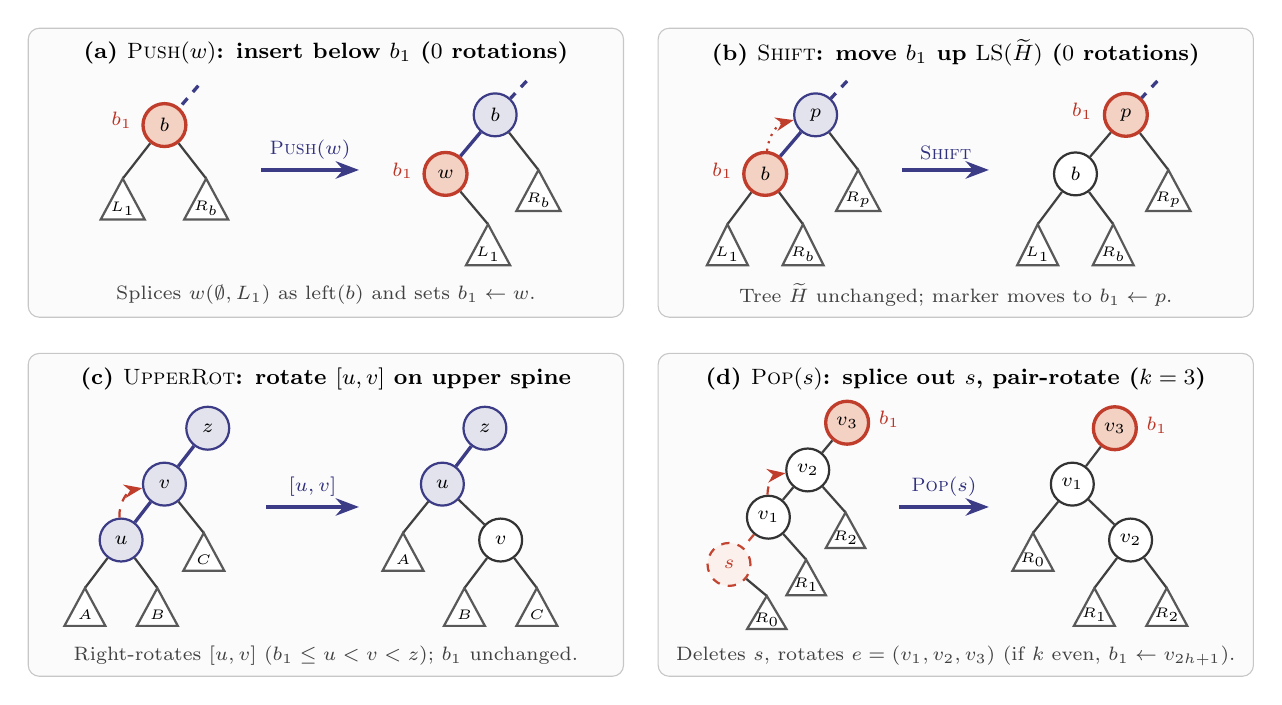
\begin{tikzpicture}[
  >=Stealth,
  bstnode/.style={circle, draw=black!80, thick, minimum size=15.5pt, inner sep=0.5pt, font=\scriptsize, fill=white},
  upnode/.style={bstnode, fill=MidnightBlue!12, draw=MidnightBlue!85},
  b1node/.style={bstnode, fill=BrickRed!16, draw=BrickRed!85, very thick},
  delnode/.style={bstnode, dashed, draw=BrickRed!80, text=BrickRed!85, fill=BrickRed!5},
  edge/.style={thick, draw=black!75},
  upedge/.style={very thick, draw=MidnightBlue!85},
  rotarc/.style={->, thick, dashed, draw=BrickRed!85},
  panelbox/.style={rounded corners=4pt, draw=black!22, fill=black!1.5}
]
  % ==================== Panel (a): PUSH(w) ====================
  \begin{scope}[xshift=0cm, yshift=0cm]
    \draw[panelbox] (-3.78, -0.42) rectangle (3.78, 3.25);
    \node[font=\footnotesize\bfseries] at (0, 2.94) {(a) $\PUSH(w)$: insert below $b_1$ ($0$ rotations)};

    % Before
    \node[b1node] (ab1) at (-2.05, 2.02) {$b$};
    \node[font=\scriptsize, text=BrickRed!90, anchor=east] at (-2.34, 2.08) {$b_1$};
    \draw[upedge, dashed] (-1.62, 2.52) -- (ab1);
    % Left triangle L_1
    \draw[edge] (ab1) -- (-2.58, 1.34);
    \draw[thick, draw=black!65, fill=white] (-2.58, 1.34) -- (-2.86, 0.82) -- (-2.30, 0.82) -- cycle;
    \node[font=\tiny] at (-2.58, 0.96) {$L_1$};
    % Right triangle R_b
    \draw[edge] (ab1) -- (-1.52, 1.34);
    \draw[thick, draw=black!65, fill=white] (-1.52, 1.34) -- (-1.80, 0.82) -- (-1.24, 0.82) -- cycle;
    \node[font=\tiny] at (-1.52, 0.96) {$R_b$};

    % Arrow
    \draw[->, very thick, MidnightBlue!85] (-0.82, 1.45) -- node[above, font=\scriptsize\bfseries, text=MidnightBlue!90] {$\PUSH(w)$} (0.42, 1.45);

    % After
    \node[upnode] (ab2) at (2.15, 2.15) {$b$};
    \draw[upedge, dashed] (2.55, 2.58) -- (ab2);
    \node[b1node] (aw) at (1.52, 1.40) {$w$};
    \node[font=\scriptsize, text=BrickRed!90, anchor=east] at (1.23, 1.44) {$b_1$};
    \draw[upedge] (ab2) -- (aw);
    % Right triangle R_b of b
    \draw[edge] (ab2) -- (2.70, 1.45);
    \draw[thick, draw=black!65, fill=white] (2.70, 1.45) -- (2.42, 0.93) -- (2.98, 0.93) -- cycle;
    \node[font=\tiny] at (2.70, 1.07) {$R_b$};
    % Right triangle L_1 of w
    \draw[edge] (aw) -- (2.06, 0.76);
    \draw[thick, draw=black!65, fill=white] (2.06, 0.76) -- (1.78, 0.24) -- (2.34, 0.24) -- cycle;
    \node[font=\tiny] at (2.06, 0.38) {$L_1$};

    \node[font=\scriptsize, text=black!75] at (0, -0.14) {Splices $w(\emptyset, L_1)$ as $\mathrm{left}(b)$ and sets $b_1 \gets w$.};
  \end{scope}

  % ==================== Panel (b): SHIFT ====================
  \begin{scope}[xshift=8.00cm, yshift=0cm]
    \draw[panelbox] (-3.78, -0.42) rectangle (3.78, 3.25);
    \node[font=\footnotesize\bfseries] at (0, 2.94) {(b) $\SHIFT$: move $b_1$ up $\LS(\widetilde{H})$ ($0$ rotations)};

    % Before
    \node[upnode] (bp1) at (-1.78, 2.15) {$p$};
    \draw[upedge, dashed] (-1.38, 2.58) -- (bp1);
    \node[b1node] (bb1) at (-2.42, 1.40) {$b$};
    \node[font=\scriptsize, text=BrickRed!90, anchor=east] at (-2.71, 1.44) {$b_1$};
    \draw[upedge] (bp1) -- (bb1);
    \draw[->, thick, dotted, draw=BrickRed!85] (bb1) to[bend left=36] (bp1);
    % Right triangle R_p
    \draw[edge] (bp1) -- (-1.24, 1.45);
    \draw[thick, draw=black!65, fill=white] (-1.24, 1.45) -- (-1.52, 0.93) -- (-0.96, 0.93) -- cycle;
    \node[font=\tiny] at (-1.24, 1.07) {$R_p$};
    % Subtrees of b
    \draw[edge] (bb1) -- (-2.90, 0.76);
    \draw[thick, draw=black!65, fill=white] (-2.90, 0.76) -- (-3.16, 0.24) -- (-2.64, 0.24) -- cycle;
    \node[font=\tiny] at (-2.90, 0.38) {$L_1$};
    \draw[edge] (bb1) -- (-1.94, 0.76);
    \draw[thick, draw=black!65, fill=white] (-1.94, 0.76) -- (-2.20, 0.24) -- (-1.68, 0.24) -- cycle;
    \node[font=\tiny] at (-1.94, 0.38) {$R_b$};

    % Arrow
    \draw[->, very thick, MidnightBlue!85] (-0.68, 1.45) -- node[above, font=\scriptsize\bfseries, text=MidnightBlue!90] {$\SHIFT$} (0.42, 1.45);

    % After
    \node[b1node] (bp2) at (2.16, 2.15) {$p$};
    \node[font=\scriptsize, text=BrickRed!90, anchor=east] at (1.86, 2.20) {$b_1$};
    \draw[upedge, dashed] (2.56, 2.58) -- (bp2);
    \node[bstnode] (bb2) at (1.52, 1.40) {$b$};
    \draw[edge] (bp2) -- (bb2);
    % Right triangle R_p
    \draw[edge] (bp2) -- (2.70, 1.45);
    \draw[thick, draw=black!65, fill=white] (2.70, 1.45) -- (2.42, 0.93) -- (2.98, 0.93) -- cycle;
    \node[font=\tiny] at (2.70, 1.07) {$R_p$};
    % Subtrees of b
    \draw[edge] (bb2) -- (1.04, 0.76);
    \draw[thick, draw=black!65, fill=white] (1.04, 0.76) -- (0.78, 0.24) -- (1.30, 0.24) -- cycle;
    \node[font=\tiny] at (1.04, 0.38) {$L_1$};
    \draw[edge] (bb2) -- (2.00, 0.76);
    \draw[thick, draw=black!65, fill=white] (2.00, 0.76) -- (1.74, 0.24) -- (2.26, 0.24) -- cycle;
    \node[font=\tiny] at (2.00, 0.38) {$R_b$};

    \node[font=\scriptsize, text=black!75] at (0, -0.14) {Tree $\widetilde{H}$ unchanged; marker moves to $b_1 \gets p$.};
  \end{scope}

  % ==================== Panel (c): UPPERROT ====================
  \begin{scope}[xshift=0cm, yshift=-4.28cm]
    \draw[panelbox] (-3.78, -0.70) rectangle (3.78, 3.40);
    \node[font=\footnotesize\bfseries] at (0, 3.08) {(c) $\UPROT$: rotate $[u, v]$ on upper spine};

    % Before
    \node[upnode] (cz1) at (-1.50, 2.45) {$z$};
    \node[upnode] (cv1) at (-2.05, 1.74) {$v$};
    \node[upnode] (cu1) at (-2.60, 1.03) {$u$};
    \draw[upedge] (cz1) -- (cv1);
    \draw[upedge] (cv1) -- (cu1);
    \draw[rotarc] (cu1) to[bend left=42] (cv1);
    % Subtrees A, B, C
    \draw[edge] (cu1) -- (-3.06, 0.42);
    \draw[thick, draw=black!65, fill=white] (-3.06, 0.42) -- (-3.32, -0.06) -- (-2.80, -0.06) -- cycle;
    \node[font=\tiny] at (-3.06, 0.08) {$A$};
    \draw[edge] (cu1) -- (-2.14, 0.42);
    \draw[thick, draw=black!65, fill=white] (-2.14, 0.42) -- (-2.40, -0.06) -- (-1.88, -0.06) -- cycle;
    \node[font=\tiny] at (-2.14, 0.08) {$B$};
    \draw[edge] (cv1) -- (-1.55, 1.12);
    \draw[thick, draw=black!65, fill=white] (-1.55, 1.12) -- (-1.81, 0.64) -- (-1.29, 0.64) -- cycle;
    \node[font=\tiny] at (-1.55, 0.78) {$C$};

    % Arrow
    \draw[->, very thick, MidnightBlue!85] (-0.76, 1.45) -- node[above, font=\scriptsize\bfseries, text=MidnightBlue!90] {$[u, v]$} (0.42, 1.45);

    % After
    \node[upnode] (cz2) at (2.02, 2.45) {$z$};
    \node[upnode] (cu2) at (1.48, 1.74) {$u$};
    \node[bstnode] (cv2) at (2.22, 1.03) {$v$};
    \draw[upedge] (cz2) -- (cu2);
    \draw[edge] (cu2) -- (cv2);
    % Subtrees A, B, C
    \draw[edge] (cu2) -- (0.98, 1.12);
    \draw[thick, draw=black!65, fill=white] (0.98, 1.12) -- (0.72, 0.64) -- (1.24, 0.64) -- cycle;
    \node[font=\tiny] at (0.98, 0.78) {$A$};
    \draw[edge] (cv2) -- (1.76, 0.42);
    \draw[thick, draw=black!65, fill=white] (1.76, 0.42) -- (1.50, -0.06) -- (2.02, -0.06) -- cycle;
    \node[font=\tiny] at (1.76, 0.08) {$B$};
    \draw[edge] (cv2) -- (2.68, 0.42);
    \draw[thick, draw=black!65, fill=white] (2.68, 0.42) -- (2.42, -0.06) -- (2.94, -0.06) -- cycle;
    \node[font=\tiny] at (2.68, 0.08) {$C$};

    \node[font=\scriptsize, text=black!75] at (0, -0.44) {Right-rotates $[u, v]$ ($b_1 \le u < v < z$); $b_1$ unchanged.};
  \end{scope}

  % ==================== Panel (d): POP(s) ====================
  \begin{scope}[xshift=8.00cm, yshift=-4.28cm]
    \draw[panelbox] (-3.78, -0.70) rectangle (3.78, 3.40);
    \node[font=\footnotesize\bfseries] at (0, 3.08) {(d) $\POP(s)$: splice out $s$, pair-rotate ($k = 3$)};

    % Before
    \node[b1node] (dv3) at (-1.38, 2.52) {$v_3$};
    \node[font=\scriptsize, text=BrickRed!90, anchor=west] at (-1.10, 2.56) {$b_1$};
    \node[bstnode] (dv2) at (-1.88, 1.92) {$v_2$};
    \node[bstnode] (dv1) at (-2.38, 1.32) {$v_1$};
    \node[delnode] (ds)  at (-2.88, 0.72) {$s$};
    \draw[edge] (dv3) -- (dv2);
    \draw[edge] (dv2) -- (dv1);
    \draw[edge, dashed, draw=BrickRed!75] (dv1) -- (ds);
    \draw[rotarc] (dv1) to[bend left=42] (dv2);
    % Right triangles R_2, R_1, R_0
    \draw[edge] (dv2) -- (-1.40, 1.38);
    \draw[thick, draw=black!65, fill=white] (-1.40, 1.38) -- (-1.65, 0.93) -- (-1.15, 0.93) -- cycle;
    \node[font=\tiny] at (-1.40, 1.06) {$R_2$};
    \draw[edge] (dv1) -- (-1.90, 0.78);
    \draw[thick, draw=black!65, fill=white] (-1.90, 0.78) -- (-2.15, 0.33) -- (-1.65, 0.33) -- cycle;
    \node[font=\tiny] at (-1.90, 0.46) {$R_1$};
    \draw[edge] (ds) -- (-2.40, 0.32);
    \draw[thick, draw=black!65, fill=white] (-2.40, 0.32) -- (-2.65, -0.10) -- (-2.15, -0.10) -- cycle;
    \node[font=\tiny] at (-2.40, 0.02) {$R_0$};

    % Arrow
    \draw[->, very thick, MidnightBlue!85] (-0.72, 1.45) -- node[above, font=\scriptsize\bfseries, text=MidnightBlue!90] {$\POP(s)$} (0.42, 1.45);

    % After
    \node[b1node] (dv3a) at (2.02, 2.45) {$v_3$};
    \node[font=\scriptsize, text=BrickRed!90, anchor=west] at (2.30, 2.49) {$b_1$};
    \node[bstnode] (dv1a) at (1.48, 1.74) {$v_1$};
    \node[bstnode] (dv2a) at (2.22, 1.03) {$v_2$};
    \draw[edge] (dv3a) -- (dv1a);
    \draw[edge] (dv1a) -- (dv2a);
    % Subtrees R_0, R_1, R_2
    \draw[edge] (dv1a) -- (0.98, 1.12);
    \draw[thick, draw=black!65, fill=white] (0.98, 1.12) -- (0.72, 0.64) -- (1.24, 0.64) -- cycle;
    \node[font=\tiny] at (0.98, 0.78) {$R_0$};
    \draw[edge] (dv2a) -- (1.76, 0.42);
    \draw[thick, draw=black!65, fill=white] (1.76, 0.42) -- (1.50, -0.06) -- (2.02, -0.06) -- cycle;
    \node[font=\tiny] at (1.76, 0.08) {$R_1$};
    \draw[edge] (dv2a) -- (2.68, 0.42);
    \draw[thick, draw=black!65, fill=white] (2.68, 0.42) -- (2.42, -0.06) -- (2.94, -0.06) -- cycle;
    \node[font=\tiny] at (2.68, 0.08) {$R_2$};

    \node[font=\scriptsize, text=black!75] at (0, -0.44) {Deletes $s$, rotates $e=(v_1,v_2,v_3)$ (if $k$ even, $b_1 \gets v_{2h+1}$).};
  \end{scope}
\end{tikzpicture}
\caption{The four operations of a folded $\POP$ process $(\widetilde{H}, b_1)$ (Definition~\ref{def:folded-pop}), with upper-spine vertices ($> b_1$) shaded blue and the fold boundary $b_1$ shaded red: (a)~$\PUSH(w)$ splices $w(\emptyset, L_1)$ directly below $b_1^{\mathrm{old}}$ and moves $b_1$ to $w$; (b)~$\SHIFT$ leaves $\widetilde{H}$ unchanged and moves $b_1$ to its parent on $\LS(\widetilde{H})$; (c)~$\UPROT$ performs one right rotation $[u, v]$ on the upper spine ($b_1 \le u < v < \mathrm{root}$) without changing $b_1$; (d)~$\POP(s)$ splices out $s = \min V_{s^-}$ and performs $h = \max(0, \lfloor(k-1)/2\rfloor)$ disjoint right rotations $[v_1, v_2], \dots, [v_{2h-1}, v_{2h}]$ strictly below $v_{2h+1}$.}
\label{fig:folded-ops}
\end{figure}

\begin{theorem}[Reduction to the Folded $\POP$ Process]
\label{thm:mod1-reduction}
There exists an absolute constant $C_{\mathrm{red}} > 0$ such that for every $n$-node BST $T_0$ ($n \ge 0$) and every valid $m$-operation deque sequence $S$ ($m \ge 0$) with $d_L$ $\POP$s and $d_R$ $\EJECT$s, there exist $\widetilde{H}_L$ and $\widetilde{H}_R$---where $\widetilde{H}_L$ is a folded $\POP$ process of size $d_L$ when $d_L \ge 1$ (setting $\widetilde{H}_L := \emptyset$ with $J(\emptyset) := 0$ when $d_L = 0$), and symmetrically for $\widetilde{H}_R$ and $d_R$---satisfying
\[
\Rot(T_0, S) \;\le\; 2\,J(\widetilde{H}_L) + 2\,J(\widetilde{H}_R) + C_{\mathrm{red}}(n + m).
\]
\end{theorem}

\paragraph{Example (spine folding and folded operations on $P = 7$ keys).}
Figure~\ref{fig:folded-pop} illustrates how a one-sided BST $H$ on $\{1, \dots, 7\}$ with right spine $\RS(H) = (4 < 6 < 7)$ and left subtrees $L_1 = 3\big(2(1, \emptyset), \emptyset\big)$, $L_2 = 5(\emptyset, \emptyset)$, and $L_3 = \emptyset$ folds upside-down into $(\widetilde{H}, b_1 = 4)$ with a single left spine $\LS(\widetilde{H}) = (1 < 2 < 3 < 4 < 6 < 7)$:
\begin{itemize}[leftmargin=2em, itemsep=1pt]
  \item \emph{$\PUSH$:} If key $1$ were not yet present (so $L_1^{\mathrm{old}} = 3(2, \emptyset)$ under $b_1^{\mathrm{old}} = 4$), executing $\PUSH(1)$ would splice $1\big(\emptyset, 3(2, \emptyset)\big)$ directly below $4$ and move the fold boundary to $b_1^{\mathrm{new}} = 1$.
  \item \emph{$\SHIFT$:} A root left rotation $[6, 4]$ on $\RS(H)$ becomes $\SHIFT$ on $(\widetilde{H}, b_1 = 4)$: the BST $\widetilde{H}$ is unchanged and $b_1$ steps up $\LS(\widetilde{H})$ from $4$ to $6$.
  \item \emph{$\UPROT$:} A deeper left rotation $[7, 6]$ on $\RS(H)$ becomes $\UPROT$: it performs the upper-spine right rotation $[4, 6]$ strictly below $7$ on $\widetilde{H}$ while keeping $b_1 = 4$.
  \item \emph{$\POP(1)$:} On the pictured $(\widetilde{H}, b_1 = 4)$, $\POP(1)$ sees lower-spine subpath $(v_0, v_1, v_2, v_3) = (1, 2, 3, 4)$ ($k = 3$, $h = 1$), splices out $1$, performs the single internal $\POP$ right rotation $e = (2, 3, 4) \in \mathcal{R}_{\mathrm{int}}(\widetilde{H})$ strictly below $b_1 = 4$, and keeps $b_1 = 4$.
\end{itemize}

\begin{figure}[ht]
\centering
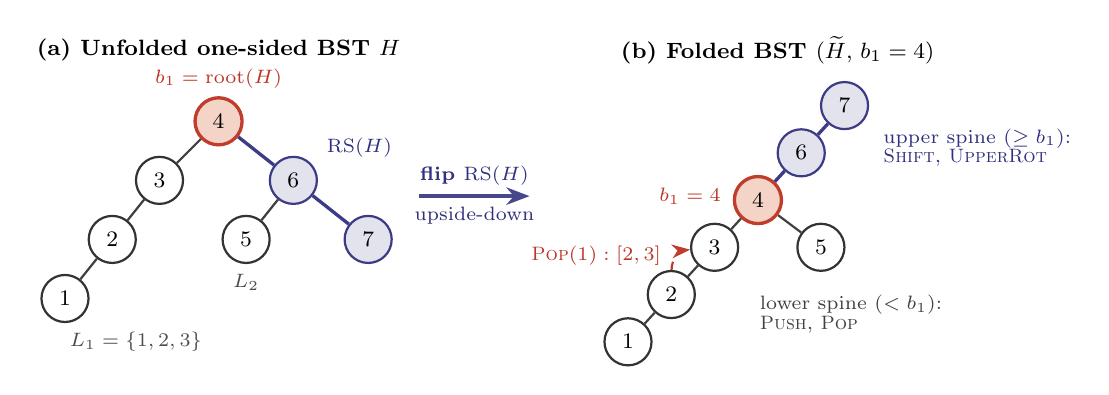
\begin{tikzpicture}[
  >=Stealth,
  bstnode/.style={circle, draw=black!80, thick, minimum size=17pt, inner sep=1pt, font=\footnotesize, fill=white},
  rsnode/.style={bstnode, fill=MidnightBlue!12, draw=MidnightBlue!85},
  b1node/.style={bstnode, fill=BrickRed!15, draw=BrickRed!85, very thick},
  edge/.style={thick, draw=black!75},
  rsedge/.style={very thick, draw=MidnightBlue!85},
  rotarc/.style={->, thick, dashed, draw=BrickRed!85}
]
  % ---------------- Panel (a): Unfolded BST H ----------------
  \begin{scope}[xshift=0cm]
    \node[font=\footnotesize\bfseries] at (0.0, 3.45) {(a) Unfolded one-sided BST $H$};
    \node[b1node] (h4) at (0.0, 2.55) {$4$};
    \node[rsnode] (h6) at (0.95, 1.80) {$6$};
    \node[rsnode] (h7) at (1.90, 1.05) {$7$};
    \node[bstnode] (h3) at (-0.75, 1.80) {$3$};
    \node[bstnode] (h2) at (-1.35, 1.05) {$2$};
    \node[bstnode] (h1) at (-1.95, 0.30) {$1$};
    \node[bstnode] (h5) at (0.35, 1.05) {$5$};

    \draw[rsedge] (h4) -- (h6);
    \draw[rsedge] (h6) -- (h7);
    \draw[edge] (h4) -- (h3);
    \draw[edge] (h3) -- (h2);
    \draw[edge] (h2) -- (h1);
    \draw[edge] (h6) -- (h5);

    \node[font=\scriptsize, text=MidnightBlue!90, anchor=west] at (1.25, 2.22) {$\RS(H)$};
    \node[font=\scriptsize, text=BrickRed!90, anchor=south] at (0.0, 2.85) {$b_1 = \mathrm{root}(H)$};
    \node[font=\scriptsize, text=black!70] at (-1.05, -0.25) {$L_1 = \{1,2,3\}$};
    \node[font=\scriptsize, text=black!70] at (0.35, 0.50) {$L_2$};
  \end{scope}

  % Folding arrow
  \draw[->, very thick, MidnightBlue!80] (2.55, 1.60) -- node[above, font=\scriptsize\bfseries, text=MidnightBlue!90] {flip $\RS(H)$} node[below, font=\scriptsize, text=MidnightBlue!90] {upside-down} (3.95, 1.60);

  % ---------------- Panel (b): Folded BST H_tilde ----------------
  \begin{scope}[xshift=7.30cm]
    \node[font=\footnotesize\bfseries] at (-0.20, 3.45) {(b) Folded BST $(\widetilde{H},\, b_1 = 4)$};
    \node[rsnode] (f7) at (0.65, 2.75) {$7$};
    \node[rsnode] (f6) at (0.10, 2.15) {$6$};
    \node[b1node] (f4) at (-0.45, 1.55) {$4$};
    \node[bstnode] (f5) at (0.35, 0.95) {$5$};
    \node[bstnode] (f3) at (-1.00, 0.95) {$3$};
    \node[bstnode] (f2) at (-1.55, 0.35) {$2$};
    \node[bstnode] (f1) at (-2.10, -0.25) {$1$};

    \draw[rsedge] (f7) -- (f6);
    \draw[rsedge] (f6) -- (f4);
    \draw[edge] (f4) -- (f5);
    \draw[edge] (f4) -- (f3);
    \draw[edge] (f3) -- (f2);
    \draw[edge] (f2) -- (f1);

    \node[font=\scriptsize, text=BrickRed!90, anchor=east] at (-0.80, 1.60) {$b_1 = 4$};
    \node[font=\scriptsize, text=MidnightBlue!90, anchor=west, align=left] at (1.02, 2.22) {upper spine ($\ge b_1$):\\[-1pt]$\SHIFT$, $\UPROT$};
    \node[font=\scriptsize, text=black!75, anchor=west, align=left] at (-0.55, 0.10) {lower spine ($< b_1$):\\[-1pt]$\PUSH$, $\POP$};
    \draw[rotarc] (f2) to[bend left=42] node[left=2pt, font=\scriptsize, text=BrickRed!90] {$\POP(1): [2,3]$} (f3);
  \end{scope}
\end{tikzpicture}
\caption{Spine folding on $P = 7$ keys (Section~\ref{subsec:folded-laws}): flipping the right spine $\RS(H) = (4 < 6 < 7)$ of the unfolded one-sided BST $H$ in~(a) upside-down onto the top of $\LS(\widetilde{H})$ produces the folded BST $(\widetilde{H}, b_1 = 4)$ in~(b), separating $\LS(\widetilde{H})$ at $b_1 = 4$ into the upper spine $\{4, 6, 7\}$ and the lower spine $\{1, 2, 3\}$.}
\label{fig:folded-pop}
\end{figure}

\paragraph{Proof overview.}
In a general two-sided execution $(T_0, S)$, $\POP$s and $\EJECT$s interact across arbitrary interleavings of $\PUSH$ and $\INJECT$. Whereas Sundar~\cite[Section~3, Theorem~7]{Sundar1992} and Pettie~\cite[Section~2]{Pettie2008} reduce two-sided deques to one-sided half-tree subproblems via size-halving epochs, we observe that because insertions occur only at the global extrema, an \emph{offline nested-interval key assignment} (Lemma~\ref{lem:nested-keys}) partitions all at most $n + m$ vertices ever present globally---with \emph{no epochs}---into a \emph{three-way key partition} $V_L < V_M < V_R$: the $d_L$ keys deleted by $\POP$ (in deletion order), the $n + m - 2d$ keys surviving in $T_m$ ($d = d_L + d_R$), and the $d_R$ keys deleted by $\EJECT$ (in reverse deletion order).

Restricting $T_t$ to $V_L, V_M, V_R$ via $\LCA$-closed projection (Lemma~\ref{lem:projection-stub}) gives three induced BSTs $(U_t, M_t, W_t)$. By the path-halving and cascade equivalence of $\POP$ and $\EJECT$ (Lemma~\ref{lem:cascade-equiv}; cf.~\cite{TarjanVanLeeuwen1984,Lucas1990,Lucas1992}, \cite[Section~3, Lemma~10]{Sundar1992}, and~\cite[Section~2, Observation~2.1]{Pettie2008}), each $\POP$ splices out $\min V(T)$ and performs vertex-disjoint paired right rotations $[v_1, v_2], [v_3, v_4], \dots$ up $\LS(T)$. Tracking the joint spine potential $|\LS(M_t)| + |\RS(M_t)| + |\RS(U_t)| + |\LS(W_t)|$ (Lemma~\ref{lem:spine-accounting}) pays $O(n + m)$ for all rotations touching $V_M$, straddling partition boundaries, or rotating $\LS(W_t)$ during $\POP$s, while bounding $\EJECT$-induced left rotations on $\RS(U_t)$ to $\max(0, 2d_L - 2)$. Prepending reverse-spine initialization and a right-spine tail of future $\INJECT$s (Lemma~\ref{lem:emptying-sim}) and applying Pettie's spine-folding bijection~\cite[Section~2, Observation~2.1 and Figure~2]{Pettie2008} in Section~\ref{subsec:folded-laws} then proves Theorem~\ref{thm:mod1-reduction} and establishes three structural laws of $\widetilde{H}$ (Lemma~\ref{lem:folded-laws}) used in Section~\ref{sec:scale-tree} (routine verifications of Lemmas~\ref{lem:projection-stub}, \ref{lem:cascade-equiv}, and~\ref{lem:emptying-sim} and the operation-by-operation check of the spine-folding bijection are deferred to Appendix~\ref{app:reduction-proofs}).

\subsection{BST Interval Projections and Cascade Equivalence}
\label{subsec:projections}

For any rooted BST $T$ with distinct real keys in symmetric order (in-order), we write $V(T)$ for its vertex (key) set, $T_v$ for the subtree rooted at $v \in V(T)$, and $u(A, B)$ for the BST rooted at $u$ with left subtree $A = \mathrm{left}_T(u)$ and right subtree $B = \mathrm{right}_T(u)$. Recall that $\LS(T)$ and $\RS(T)$ denote the left and right spines of $T$ (visited from $\mathrm{root}(T)$ by following left or right child pointers, respectively, with $\LS(\emptyset) = \RS(\emptyset) = \emptyset$). Following Sundar~\cite[Section~1.2]{Sundar1992}, define the \emph{left depth} $\ld_T(v)$ of $v \in V(T)$ to be the number of left-child edges on the root-to-$v$ path in $T$ (so $\ld_T(v) = 0$ if and only if $v \in \RS(T)$). Under any right single rotation $[u, v]$ replacing $v\big(u(A, M), R\big)$ with $u\big(A, v(M, R)\big)$, $\ld(w)$ decreases by~$1$ for every $w \in \{u\} \cup V(A)$ and remains unchanged for every $w \in \{v\} \cup V(M) \cup V(R) \cup (V(T) \setminus V(T_v))$; moreover, $|\LS(T)|$ decreases by~$1$ if $v \in \LS(T)$ (removing $v$ from $\LS(T)$ while keeping $u$ and $\LS(A)$) and by~$0$ otherwise. Symmetrically, any left single rotation $[v, u]$ decreases $|\RS(T)|$ by~$1$ if $u \in \RS(T)$ and by~$0$ otherwise.

To follow how a subset of keys $\mathcal{S} \subseteq \mathbb{R}$ evolves inside a larger dynamic BST $T$---both for contiguous key intervals (as in~\cite{Tarjan1985} and~\cite[Section~2.1]{Sundar1992}) and for non-contiguous summary subsets in Section~\ref{sec:cascades}---we want to contract away every vertex outside $\mathcal{S}$ and keep a valid BST on the remaining keys $V(T) \cap \mathcal{S}$. Removing a vertex $u \notin \mathcal{S}$ without creating a two-child conflict requires that at most one of $u$'s two subtrees contain keys from $\mathcal{S}$, which holds at every $u \notin \mathcal{S}$ precisely when $\mathcal{S}$ is closed under lowest common ancestors.

\begin{definition*}[$\LCA$-Closed Subsets and Induced BSTs]
Let $T$ be a BST with real keys and let $\mathcal{S} \subseteq \mathbb{R}$ be any subset of keys; write $\LCA_T(x, y)$ for the lowest common ancestor of $x, y \in V(T)$ in $T$.
\begin{enumerate}[label=(\arabic*), leftmargin=2em, itemsep=2pt]
  \item \emph{$\LCA$-closure.} We say $\mathcal{S}$ is \emph{$\LCA$-closed} in $T$ if for every pair of vertices $x, y \in V(T) \cap \mathcal{S}$, their lowest common ancestor $\LCA_T(x, y)$ also belongs to $\mathcal{S}$. (For instance, every contiguous interval $I \subseteq \mathbb{R}$ is $\LCA$-closed in every BST $T$, since symmetric order forces $x \le \LCA_T(x, y) \le y$ whenever $x \le y$.)
  \item \emph{Induced BST $T|_{\mathcal{S}}$.} Suppose $\mathcal{S}$ is $\LCA$-closed in $T$. For any vertex $u \notin \mathcal{S}$ with subtrees $A = \mathrm{left}_T(u)$ and $B = \mathrm{right}_T(u)$, keys of $\mathcal{S}$ cannot appear in both $A$ and $B$ (otherwise $a \in V(A) \cap \mathcal{S}$ and $b \in V(B) \cap \mathcal{S}$ would force $\LCA_T(a, b) = u \notin \mathcal{S}$). Keeping each $u \in \mathcal{S}$ and replacing each $u \notin \mathcal{S}$ by whichever restricted child subtree is non-empty (or $\emptyset$ if neither intersects $\mathcal{S}$) defines the \emph{induced BST} $T|_{\mathcal{S}}$ on $V(T) \cap \mathcal{S}$ recursively via $\emptyset|_{\mathcal{S}} := \emptyset$ and
  \[
  u(A, B)\big|_{\mathcal{S}} \;:=\;
  \begin{cases}
  u\big(A|_{\mathcal{S}},\, B|_{\mathcal{S}}\big) & \text{if } u \in \mathcal{S},\\
  A|_{\mathcal{S}} & \text{if } u \notin \mathcal{S} \text{ and } V(B) \cap \mathcal{S} = \emptyset,\\
  B|_{\mathcal{S}} & \text{if } u \notin \mathcal{S} \text{ and } V(B) \cap \mathcal{S} \ne \emptyset \quad (\text{in which case } V(A) \cap \mathcal{S} = \emptyset).
  \end{cases}
  \]
\end{enumerate}
By structural induction, $T|_{\mathcal{S}}$ is a valid BST with $V(T|_{\mathcal{S}}) = V(T) \cap \mathcal{S}$ that preserves exact ancestor--descendant and left/right-subtree relations on $V(T) \cap \mathcal{S}$.
\end{definition*}

\begin{lemma}[BST Projection Under Rotations and Extremum Splicing]
\label{lem:projection-stub}
Let $T$ be a BST and let $\mathcal{S} \subseteq \mathbb{R}$ be $\LCA$-closed in $T$.
\begin{enumerate}[label=(\arabic*)]
  \item Suppose $T'$ is obtained from $T$ by a single rotation $[x, y]$ and $\mathcal{S}$ is also $\LCA$-closed in $T'$. If $x, y \in \mathcal{S}$, then $T'|_{\mathcal{S}}$ is obtained from $T|_{\mathcal{S}}$ by the single rotation $[x, y]$; if $\{x, y\} \not\subseteq \mathcal{S}$, then $T'|_{\mathcal{S}} = T|_{\mathcal{S}}$.
  \item Suppose $T \ne \emptyset$, and let $T'$ be obtained from $T$ by splicing out $x_{\min} := \min V(T)$ (replacing $x_{\min}(\emptyset, R)$ with $R$) or $x_{\max} := \max V(T)$ (replacing $x_{\max}(L, \emptyset)$ with $L$). Then $\mathcal{S}$ remains $\LCA$-closed in $T'$; if the spliced-out extremum lies in $\mathcal{S}$, it is the corresponding extremum of $T|_{\mathcal{S}}$ and $T'|_{\mathcal{S}}$ is obtained by splicing it out of $T|_{\mathcal{S}}$, whereas otherwise $T'|_{\mathcal{S}} = T|_{\mathcal{S}}$.
\end{enumerate}
\end{lemma}

The four-case verification of Lemma~\ref{lem:projection-stub} is deferred to Appendix~\ref{app:reduction-proofs}. Next, we record the standard equivalence between bottom-up extremum splaying and vertex-disjoint paired single rotations along the spine, adapting the path-halving and cascade simplifications of~\cite{TarjanVanLeeuwen1984}, \cite[Section~2 and Section~3, Lemma~10]{Sundar1992}, \cite{Lucas1992}, and~\cite[Section~2, Observation~2.1]{Pettie2008} directly to arbitrary two-sided BSTs.

\begin{lemma}[Cascade Equivalence of $\POP$ and $\EJECT$]
\label{lem:cascade-equiv}
Let $T$ be a non-empty BST with left spine $\LS(T) = (v_0 < v_1 < \dots < v_k)$ from $v_0 = \min V(T)$ to $v_k = \mathrm{root}(T)$ ($k \ge 0$), and set $r := \lfloor k / 2 \rfloor$. Executing $\POP$ on $T$ performs $k \in \{2r, 2r + 1\}$ single rotations and produces the exact same BST as first splicing out $v_0$ (replacing $v_0(\emptyset, R_0)$ with $R_0 := \mathrm{right}_T(v_0)$) and then performing the $r$ vertex-disjoint right single rotations $[v_1, v_2], [v_3, v_4], \dots, [v_{2r-1}, v_{2r}]$. Symmetrically, if $\RS(T) = (u_k < \dots < u_1 < u_0)$ with $u_0 = \max V(T)$ and $r := \lfloor k / 2 \rfloor$, executing $\EJECT$ on $T$ performs $k \in \{2r, 2r + 1\}$ single rotations and produces the exact same BST as splicing out $u_0$ and performing the $r$ vertex-disjoint left single rotations $[u_1, u_2], [u_3, u_4], \dots, [u_{2r-1}, u_{2r}]$.
\end{lemma}

The inductive check of Lemma~\ref{lem:cascade-equiv} is given in Appendix~\ref{app:reduction-proofs}.


\subsection{Three-Way Key Partition via Offline Nested-Interval Assignment}
\label{subsec:three-way-partition}

Fix an $n$-node initial BST $T_0$ ($n \ge 0$) and a valid sequence $S = (\mathrm{op}_1, \dots, \mathrm{op}_m)$ of $m \ge 0$ deque operations producing intermediate trees $T_0, T_1, \dots, T_m$, with $d_L$ $\POP$ deletions, $d_R$ $\EJECT$ deletions, $d := d_L + d_R$, and $m - d$ insertions ($\PUSH$ and $\INJECT$). Because deque operations depend only on the relative symmetric order of active keys, we may choose any real keys for the initial vertices and inserted vertices consistent with symmetric order at insertion time. Unlike the size-halving epoch reductions of Sundar~\cite[Section~3, Theorem~7]{Sundar1992} and Pettie~\cite[Section~2]{Pettie2008}, the following offline key assignment separates all $n + m - d$ vertices ever present globally into a single static three-way partition without epochs.

\begin{lemma}[Offline Nested-Interval Three-Way Key Assignment]
\label{lem:nested-keys}
Let $\mathcal{V}$ be the set of all $n + m - d \le n + m$ vertices ever present across $(T_0, S)$. There exists a static key assignment $\kappa : \mathcal{V} \to \mathbb{R}$ (with real thresholds $L_m < R_m$) under which every $T_t$ ($0 \le t \le m$) is a valid BST and $\kappa(\mathcal{V}) = V_L \sqcup V_M \sqcup V_R$ partitions into:
\begin{itemize}[leftmargin=2em]
  \item $V_L \subseteq (-\infty, L_m]$ ($|V_L| = d_L$), the keys deleted by $\POP$, ordered in exact chronological $\POP$ deletion order;
  \item $V_M := \kappa(V(T_m)) \subset (L_m, R_m)$ ($|V_M| = n + m - 2d$), the keys surviving in $T_m$;
  \item $V_R \subseteq [R_m, +\infty)$ ($|V_R| = d_R$), the keys deleted by $\EJECT$, ordered in exact reverse chronological $\EJECT$ deletion order;
\end{itemize}
so that $x < y < z$ for all $x \in V_L$, $y \in V_M$, and $z \in V_R$.
\end{lemma}

\begin{proof}
Assign the $n$ vertices of $T_0$ the keys $1, 2, \dots, n$ in symmetric order, and maintain open bounds $(L_t, R_t)$ initialized to $(L_0, R_0) := (0, n + 1)$ so that $L_t < R_t$ and $\kappa(V(T_t)) \subset (L_t, R_t)$ for every $0 \le t \le m$:
\begin{itemize}[leftmargin=2em]
  \item If $\mathrm{op}_t = \PUSH$, keep $(L_t, R_t) := (L_{t-1}, R_{t-1})$ and assign the new key $\frac{1}{2}\big(L_{t-1} + \min \kappa(V(T_{t-1}))\big)$ when $T_{t-1} \ne \emptyset$, or $\frac{1}{2}(L_{t-1} + R_{t-1})$ when $T_{t-1} = \emptyset$.
  \item If $\mathrm{op}_t = \INJECT$, keep $(L_t, R_t) := (L_{t-1}, R_{t-1})$ and assign the new key $\frac{1}{2}\big(\max \kappa(V(T_{t-1})) + R_{t-1}\big)$ when $T_{t-1} \ne \emptyset$, or $\frac{1}{2}(L_{t-1} + R_{t-1})$ when $T_{t-1} = \emptyset$.
  \item If $\mathrm{op}_t = \POP$ deleting $x = \min \kappa(V(T_{t-1}))$, set $(L_t, R_t) := (x, R_{t-1})$.
  \item If $\mathrm{op}_t = \EJECT$ deleting $z = \max \kappa(V(T_{t-1}))$, set $(L_t, R_t) := (L_{t-1}, z)$.
\end{itemize}
On $\POP$, $L_{t-1} < x < R_{t-1}$ and every $u \in \kappa(V(T_t)) = \kappa(V(T_{t-1})) \setminus \{x\}$ satisfies $x < u < R_{t-1}$, preserving $L_t < R_t$ and $\kappa(V(T_t)) \subset (L_t, R_t)$; $\EJECT$ is symmetric. Hence $0 = L_0 \le L_1 \le \dots \le L_m < R_m \le \dots \le R_0 = n + 1$. The $d_L$ keys deleted by $\POP$ are the strictly increasing sequence of step-ups $L_{t-1} < L_t = x \le L_m$, the $n + (m - d) - d = n + m - 2d$ surviving keys of $T_m$ lie in $(L_m, R_m)$, and the $d_R$ keys deleted by $\EJECT$ are the strictly decreasing sequence of step-downs $R_m \le z = R_t < R_{t-1}$.
\end{proof}

Identify $\mathcal{V}$ with $\kappa(\mathcal{V})$ via Lemma~\ref{lem:nested-keys}, set $I_L := (-\infty, L_m]$, $I_M := (L_m, R_m)$, and $I_R := [R_m, +\infty)$, and consider the three interval-projected BSTs $U_t := T_t|_{I_L}$, $M_t := T_t|_{I_M}$, and $W_t := T_t|_{I_R}$ ($0 \le t \le m$), which satisfy $V(U_t) = V(T_t) \cap V_L$, $V(M_t) = V(T_t) \cap V_M$, and $V(W_t) = V(T_t) \cap V_R$ (with $U_m = W_m = \emptyset$). In the cascade decomposition of Lemma~\ref{lem:cascade-equiv}, let $C_{\POP}(U)$ denote the total number of cascade right rotations $[v_{2j-1}, v_{2j}] \in V_L \times V_L$ across all $\POP$ steps, and let $C_{\EJECT}(W)$ denote the total number of cascade left rotations $[u_{2j-1}, u_{2j}] \in V_R \times V_R$ across all $\EJECT$ steps.

\begin{lemma}[Uncoupled Spine Potential Accounting]
\label{lem:spine-accounting}
Across $(T_0, S)$:
\begin{enumerate}[label=(\arabic*)]
  \item $\Rot(T_0, S) \le 2\,C_{\POP}(U) + 2\,C_{\EJECT}(W) + 9(n + m)$.
  \item $\EJECT$ steps induce at most $\max(0, 2d_L - 2)$ left single rotations on $U_t$ (each along $\RS(U_t)$), and $\POP$ steps induce at most $\max(0, 2d_R - 2)$ right single rotations on $W_t$ (each along $\LS(W_t)$).
\end{enumerate}
\end{lemma}

\begin{proof}
Define the uncoupled spine potential
\[
\Psi(t) \;:=\; |\LS(M_t)| + |\RS(M_t)| + |\RS(U_t)| + |\LS(W_t)| \;\ge\; 0 \qquad (0 \le t \le m).
\]
At $t = 0$, $\Psi(0) \le 2|V(M_0)| + |V(U_0)| + |V(W_0)| \le 2n$. At each of the $m - d$ insertion steps ($\PUSH(w)$ or $\INJECT(w)$), $T_t$ attaches $w$ as the new root with one empty subtree and $T_{t-1}$ as the other subtree, so by Lemma~\ref{lem:projection-stub} (or directly from the recursive definition of $\cdot|_{\mathcal{S}}$) the two projections not containing $w$ are unchanged while the projection containing $w$ acquires $w$ as its new root with at least one empty child subtree: if $w \in V_M$, $|\LS(M_t)| + |\RS(M_t)|$ increases by at most~$2$ ($+2$ when $M_{t-1} = \emptyset$, at most $+1$ when $M_{t-1} \ne \emptyset$); if $w \in V_L$, $|\RS(U_t)|$ changes by $+1$ on $\PUSH$ ($U_t = w(\emptyset, U_{t-1})$) and by $1 - |\RS(U_{t-1})| \le +1$ on $\INJECT$ ($U_t = w(U_{t-1}, \emptyset)$); and symmetrically $\Delta|\LS(W_t)| \le +1$ if $w \in V_R$. Hence every insertion satisfies $\Delta\Psi(t) := \Psi(t) - \Psi(t - 1) \le 2$, contributing $\sum_{t\text{ ins}} \Delta\Psi(t) \le 2(m - d)$ in total.

Now consider any $\POP$ step $t$. Since $\min V(T_{t-1}) \in V_L$ and $I_L = (-\infty, L_m]$ is downward-closed, $\LS(U_{t-1}) = \LS(T_{t-1}) \cap V_L = (v_0 < \dots < v_p)$ ($p \ge 0$) is a non-empty bottom prefix of $\LS(T_{t-1}) = (v_0 < \dots < v_k)$ ($k \ge p$). By Lemma~\ref{lem:cascade-equiv}, step $t$ performs $k \le 1 + 2 r_t$ single rotations ($r_t := \lfloor k / 2 \rfloor$) and transforms $T_{t-1}$ into $T_t$ by splicing out $v_0$ and executing $[v_1, v_2], [v_3, v_4], \dots, [v_{2r_t - 1}, v_{2r_t}]$. Decompose these $r_t$ pairs into $\lfloor p / 2 \rfloor$ internal $V_L \times V_L$ pairs, $c_t$ boundary-straddling pairs (endpoints in different parts of $V_L < V_M < V_R$), $m_t$ internal $V_M \times V_M$ pairs, and $\mathrm{opp}_t(W)$ internal $V_R \times V_R$ pairs:
\begin{itemize}[leftmargin=2em]
  \item \emph{Straddling pairs:} Along $v_1 < v_2 < \dots < v_{2r_t}$, at most one pair crosses $L_m$ and at most one pair crosses $R_m$, so $c_t \le 2$.
  \item \emph{Induced update on $U_t$:} By Lemma~\ref{lem:projection-stub}, $U_{t-1} \to U_t$ splices out $v_0 = \min V(U_{t-1})$ and executes the $\lfloor p / 2 \rfloor$ internal $V_L \times V_L$ right rotations $[v_1, v_2], \dots, [v_{2\lfloor p/2 \rfloor - 1}, v_{2\lfloor p/2 \rfloor}]$ (a standalone $\POP$ cascade on $U_{t-1}$). If $p = 0$ (which in particular holds on the $d_L$-th $\POP$, when $|V(U_{t-1})| = 1$), splicing out $v_0 = \mathrm{root}(U_{t-1})$ removes $v_0$ from $\RS(U)$ with $0$ rotations, giving $\Delta|\RS(U_t)| = -1$. If $p \ge 1$, splicing out $v_0 < v_p = \mathrm{root}(U_{t-1})$ leaves $\RS(U)$ unchanged, and among the $\lfloor p / 2 \rfloor$ vertex-disjoint right rotations on $\LS(U_{t-1})$ at most one touches $\mathrm{root}(U_{t-1})$ (adding at most one vertex to $\RS(U)$), so $\Delta|\RS(U_t)| \le +1$ in all cases.
  \item \emph{Induced updates on $M_t$ and $W_t$:} Every $y \in \LS(T_{t-1}) \cap V_M$ has all proper ancestors in $T_{t-1}$ strictly greater than $y$, so any ancestor of $y$ in $M_{t-1}$ contains $y$ in its left subtree; thus $\LS(T_{t-1}) \cap V_M \subseteq \LS(M_{t-1})$, and likewise $\LS(T_{t-1}) \cap V_R \subseteq \LS(W_{t-1})$. By Lemma~\ref{lem:projection-stub}, each of the $m_t$ vertex-disjoint pairs in $V_M \times V_M$ rotates right on $\LS(M_{t-1})$, decreasing $|\LS(M)|$ by~$1$ and increasing $|\RS(M)|$ by~$1$ only if its upper endpoint is $\mathrm{root}(M_{t-1})$ (at most one pair), giving $m_t + \Delta(|\LS(M_t)| + |\RS(M_t)|) \le 1$. Similarly, the $\mathrm{opp}_t(W)$ pairs in $V_R \times V_R$ rotate right along $\LS(W_{t-1})$, giving $\mathrm{opp}_t(W) + \Delta|\LS(W_t)| = 0$.
\end{itemize}
Combining these four estimates gives $(c_t + m_t + \mathrm{opp}_t(W)) + \Delta\Psi(t) \le 2 + 1 + 1 + 0 = 4$ on every $\POP$ step $t$, and mirror symmetry gives $(c_t + m_t + \mathrm{opp}_t(U)) + \Delta\Psi(t) \le 4$ on every $\EJECT$ step $t$ (where $\mathrm{opp}_t(U)$ counts $V_L \times V_L$ left single rotations along $\RS(U_{t-1})$, with $\mathrm{opp}_t(U) + \Delta|\RS(U_t)| = 0$).

Telescoping $\Psi(m) - \Psi(0) \ge -\Psi(0) \ge -2n$ across all $m$ operations yields
\[
\sum_{t\text{ del}} \big(c_t + m_t + \mathrm{opp}_t\big)
\;\le\; 4d + \Psi(0) + \sum_{t\text{ ins}} \Delta\Psi(t)
\;\le\; 4d + 2n + 2(m - d) \;=\; 2n + 2m + 2d.
\]
Since $\Rot(T_0, S) \le d + 2\big(C_{\POP}(U) + C_{\EJECT}(W) + \sum_{t\text{ del}}(c_t + m_t + \mathrm{opp}_t)\big)$ and $d \le m \le n + m$, we obtain $\Rot(T_0, S) \le 2\,C_{\POP}(U) + 2\,C_{\EJECT}(W) + 4n + 4m + 5d \le 2\,C_{\POP}(U) + 2\,C_{\EJECT}(W) + 9(n + m)$, proving~(1). Finally, tracking $|\RS(U_t)|$ alone shows that when $d_L = 0$ we have $U_t = \emptyset$ and $\mathrm{opp}_t(U) = 0$, whereas when $d_L \ge 1$, $|\RS(U_0)| + \sum_{t\text{ ins}} \Delta|\RS(U_t)| \le |V(U_0)| + (d_L - |V(U_0)|) = d_L$, at most $d_L - 1$ $\POP$s satisfy $\Delta|\RS(U_t)| \le +1$, the $d_L$-th $\POP$ satisfies $\Delta|\RS(U_t)| = -1$, and $|\RS(U_m)| = 0$, so $\sum_{t\text{ }\EJECT} \mathrm{opp}_t(U) \le d_L + (d_L - 1) - 1 = 2d_L - 2$; mirror symmetry bounds $\sum_{t\text{ }\POP} \mathrm{opp}_t(W) \le \max(0, 2d_R - 2)$, proving~(2).
\end{proof}


\subsection{Emptying Simulation, Spine Folding, and Structural Laws of \texorpdfstring{$\widetilde{H}$}{H-tilde}}
\label{subsec:folded-laws}

Before folding the right spine upside-down, we package the left-end subproblem $U_t$ into a clean unfolded one-sided model that starts and ends at the empty tree. A \emph{one-sided $\POP$ execution} $H$ of size $P \ge 1$ starting from $\emptyset$ on $\{1, \dots, P\}$ is a dynamic BST sequence that begins at $H = \emptyset$, ends at $H = \emptyset$, and consists of:
\begin{enumerate}[label=(\roman*), leftmargin=2em, itemsep=1pt]
  \item $P$ $\PUSH(w)$ steps ($w \in \{1, \dots, P\}$, with $w < \min V(H)$ when $H \ne \emptyset$), each attaching $w$ at the root via $H \gets w(\emptyset, H)$;
  \item $P$ $\POP$ steps deleting $s = 1, \dots, P$ in increasing order via the cascade rule of Lemma~\ref{lem:cascade-equiv} (splicing out $s = \min V(H)$ and executing $\lfloor k / 2 \rfloor$ vertex-disjoint right single rotations $[v_1, v_2], \dots$ along $\LS(H) = (v_0 < \dots < v_k)$); and
  \item $K_L \ge 0$ right-spine left single rotations $[b_{d+1}, b_d]$ along $\RS(H) = (b_1 < \dots < b_\beta)$ ($1 \le d \le \beta - 1$).
\end{enumerate}
Write $C_{\POP}(H)$ for the total number of cascade right rotations across the $P$ $\POP$ steps. Notice in three lines that $K_L < 2P$ holds automatically: $|\RS(H)|$ starts at $0$ and ends at $0$; each of the $P$ $\PUSH$es changes $|\RS(H)|$ by $+1$, each of the first $P - 1$ $\POP$s changes $|\RS(H)|$ by at most $+1$, the $P$-th $\POP$ acts on $|V(H)| = 1$ ($|\LS(H)| = 1$) and changes $|\RS(H)|$ by $-1$, and each right-spine left rotation $[b_{d+1}, b_d]$ decreases $|\RS(H)|$ by~$1$, forcing
\begin{equation}
\label{eq:KL-bound}
K_L \;\le\; P + (P - 1) - 1 \;=\; 2P - 2 \;<\; 2P.
\end{equation}

For any two BSTs $A, B$ with $\max V(A) < \min V(B)$ whenever both are non-empty, write $A \oplus_R B$ for the BST obtained by attaching $B$ in place of the rightmost external leaf of $A$ (with $\emptyset \oplus_R B := B$ and $A \oplus_R \emptyset := A$).

\begin{lemma}[Emptying One-Sided Simulation via Reverse-Spine Initialization and Right-Spine Tail]
\label{lem:emptying-sim}
\leavevmode
\begin{enumerate}[label=(\arabic*)]
  \item Any $n_0$-node BST $H_{\mathrm{init}}$ can be constructed from $\emptyset$ using $n_0$ $\PUSH$ steps, $n_0 - |\RS(H_{\mathrm{init}})|$ root right-spine left rotations $[b_2, b_1]$, and $0$ $\POP$ steps.
  \item Whenever $d_L \ge 1$ in $(T_0, S)$, relabeling $V_L$ in chronological $\POP$ deletion order to $\{1, \dots, P\}$ ($P := d_L$) yields a one-sided $\POP$ execution $H_L$ of size $P$ starting from $\emptyset$ with $C_{\POP}(U) = C_{\POP}(H_L)$ and $K_L \le 2P - 2 < 2P$.
\end{enumerate}
\end{lemma}

The proof of Lemma~\ref{lem:emptying-sim} is deferred to Appendix~\ref{app:reduction-proofs}.

\paragraph{Spine-folding bijection.}
Following Pettie~\cite[Section~2, Observation~2.1 and Figure~2]{Pettie2008} (building on Sundar~\cite[Section~3, Lemma~10]{Sundar1992} and Lucas~\cite{Lucas1990,Lucas1992}), we map any one-sided $\POP$ execution $H$ of size $P \ge 1$ starting from $\emptyset$ onto a \emph{folded $\POP$ process} $\widetilde{H}$ of size $P$ (Definition~\ref{def:folded-pop}). At any timestamp $\tau$, if $H_\tau = \emptyset$ set $\widetilde{H}_\tau := \emptyset$; if $H_\tau \ne \emptyset$ with right spine $\RS(H_\tau) = (b_1 < b_2 < \dots < b_\beta)$ ($\beta \ge 1$) and left subtrees $L_i := \mathrm{left}_{H_\tau}(b_i)$ ($1 \le i \le \beta$), define $\widetilde{H}_\tau$ and its fold boundary $b_1(\tau) := b_1 \in \LS(\widetilde{H}_\tau)$ by placing $b_\beta, b_{\beta - 1}, \dots, b_1$ down the top of $\LS(\widetilde{H}_\tau)$ with $\mathrm{root}(\widetilde{H}_\tau) := b_\beta$, $\mathrm{right}_{\widetilde{H}_\tau}(b_\beta) := \emptyset$, $\mathrm{left}_{\widetilde{H}_\tau}(b_{i+1}) := b_i$ and $\mathrm{right}_{\widetilde{H}_\tau}(b_i) := L_{i+1}$ for $1 \le i < \beta$, and $\mathrm{left}_{\widetilde{H}_\tau}(b_1) := L_1$. Because $V(L_1) < b_1 < V(L_2) < b_2 < \dots < V(L_\beta) < b_\beta$ in $H_\tau$, $\widetilde{H}_\tau$ is a valid BST on $V_\tau := V(H_\tau)$ uniquely recovering $H_\tau$ from $(\widetilde{H}_\tau, b_1(\tau))$. As verified across the four step types of $H$ ($\PUSH$, root right-spine left rotation $\mapsto \SHIFT$, deeper right-spine left rotation $\mapsto \UPROT$, and $\POP$) in Appendix~\ref{app:reduction-proofs}, $\widetilde{H}$ is a valid folded $\POP$ process of size $P$ satisfying
\begin{equation}
\label{eq:cpop-folded}
C_{\POP}(H) \;\le\; P + J(\widetilde{H}).
\end{equation}

\begin{proof}[Proof of Theorem~\ref{thm:mod1-reduction}]
By Lemma~\ref{lem:spine-accounting}(1), $\Rot(T_0, S) \le 2\,C_{\POP}(U) + 2\,C_{\EJECT}(W) + 9(n + m)$. If $d_L \ge 1$, Lemma~\ref{lem:emptying-sim}(2) and~\eqref{eq:cpop-folded} produce a folded $\POP$ process $\widetilde{H}_L$ of size $d_L$ with $C_{\POP}(U) = C_{\POP}(H_L) \le d_L + J(\widetilde{H}_L)$, whereas if $d_L = 0$ then $C_{\POP}(U) = 0 = d_L + J(\emptyset)$. Applying the same construction to the order-reversed mirror execution ($x \mapsto -x$, exchanging $\PUSH \leftrightarrow \INJECT$, $\POP \leftrightarrow \EJECT$, and left/right children) yields $\widetilde{H}_R$ of size $d_R$ (or $\emptyset$ when $d_R = 0$) with $C_{\EJECT}(W) \le d_R + J(\widetilde{H}_R)$. Since $d_L + d_R = d \le m \le n + m$, we conclude
\[
\Rot(T_0, S) \;\le\; 2\big(d_L + J(\widetilde{H}_L)\big) + 2\big(d_R + J(\widetilde{H}_R)\big) + 9(n + m) \;\le\; 2\,J(\widetilde{H}_L) + 2\,J(\widetilde{H}_R) + 11(n + m),
\]
proving Theorem~\ref{thm:mod1-reduction} with $C_{\mathrm{red}} := 11$.
\end{proof}

We close Section~\ref{sec:reduction} by recording three structural laws of any folded $\POP$ process $\widetilde{H}$ of size $P \ge 1$ (Definition~\ref{def:folded-pop}). To track how keys move upward across right rotations via a single monotone parent pointer, associate to $\widetilde{H}_\tau$ its standard \emph{first-child/right-sibling general ordered tree} $L''_\tau$ on $V_\tau \cup \{\top\}$ rooted at a sentinel super-root $\top := P + 1$ (Knuth~\cite[Section~2.3.2]{Knuth1997Vol1}): $x$ is the first child of $y \in V_\tau$ if and only if $x = \mathrm{left}_{\widetilde{H}_\tau}(y)$ (with $\mathrm{root}(\widetilde{H}_\tau)$ the first child of $\top$ when $V_\tau \ne \emptyset$), and $w$ is the immediate right sibling of $x$ if and only if $w = \mathrm{right}_{\widetilde{H}_\tau}(x)$, so the children of $y \in V_\tau$ in left-to-right order are precisely the right spine $\RS(\mathrm{left}_{\widetilde{H}_\tau}(y))$. Write $\pi_\tau : V_\tau \to V_\tau \cup \{\top\}$ for the parent map of $L''_\tau$. Directly on the BST $\widetilde{H}_\tau$, observe by induction on Definition~\ref{def:folded-pop} that whenever $V_\tau \ne \emptyset$, $\mathrm{right}_{\widetilde{H}_\tau}(\mathrm{root}(\widetilde{H}_\tau)) = \emptyset$ (every $\UPROT$ and internal $\POP$ rotation occurs strictly below $\mathrm{root}(\widetilde{H}_\tau)$), so $\mathrm{root}(\widetilde{H}_\tau)$ is the unique child of $\top$, and for every $v \in V_\tau$, $\pi_\tau(v)$ is simply the lowest ancestor $a$ of $v$ in $\widetilde{H}_\tau$ whose left subtree contains $v$ (or $\top$ when $v = \mathrm{root}(\widetilde{H}_\tau)$).

\begin{lemma}[Structural Laws of $(\widetilde{H}, L'')$]
\label{lem:folded-laws}
Let $\widetilde{H}$ be any folded $\POP$ process of size $P \ge 1$ (Definition~\ref{def:folded-pop}), with general tree $L''_\tau$ and parent map $\pi_\tau : V_\tau \to V_\tau \cup \{\top\}$ ($\top := P + 1$).
\begin{enumerate}[label=(\arabic*)]
  \item \emph{(Postorder and parent monotonicity)} At every timestamp $\tau$, $\mathrm{postorder}(L''_\tau)$ on $V_\tau$ coincides with $\textnormal{in-order}(\widetilde{H}_\tau)$, i.e., increasing key order, so $v < \pi_\tau(v)$ for all $v \in V_\tau$. Every right single rotation $[x, y]$ strictly below $z = \pi_{\tau^-}(y)$ (either an $\UPROT$ step or an internal $\POP$ rotation) updates $\pi(x) : y \mapsto z$ and leaves $\pi(w)$ unchanged for all $w \in V_\tau \setminus \{x\}$; consequently, throughout the lifetime of each $v \in \{1, \dots, P\}$, $\pi_\tau(v)$ is non-decreasing and the set of ancestors of $v$ in $L''_\tau$ shrinks monotonically.
  \item \emph{(Spine interval partition and $(x, z)$ interval-freezing)} Whenever $V_\tau \ne \emptyset$ with $\LS(\widetilde{H}_\tau) = (u_1 < \dots < u_q)$ and $u_{q+1} := P + 1$, we have $\{u_i\} \cup V(\mathrm{right}_{\widetilde{H}_\tau}(u_i)) = V_\tau \cap [u_i, u_{i+1} - 1]$ for all $1 \le i \le q$. Moreover, after any internal $\POP$ rotation $e = (x, y, z) \in \mathcal{R}_{\mathrm{int}}(\widetilde{H})$ during $\POP(s)$ ($s < x < y < z$), zero keys strictly greater than $x$ are inserted and $(x, z) \cap \LS(\widetilde{H}_\tau) = \emptyset$ throughout $[s^+, x^-]$ (so no vertex of $(x, z)$ lies on $\LS(\widetilde{H})$ during any $\UPROT$ or $\POP(s')$ up to and including $\POP(x)$).
  \item \emph{(Backward adjacent-pair injectivity)} Let $\mathcal{M}_{\mathrm{base}} \subseteq \mathcal{R}_{\mathrm{int}}(\widetilde{H})$ comprise all internal $\POP$ rotations $e = (x, y, z)$ that are either (i) the chronologically first internal $\POP$ rotation with promoted key $x$, (ii) preceded (since $x$'s previous internal $\POP$ rotation) by an $\UPROT$ step $[x, v]$ promoting $x$, or (iii) preceded by an internal $\POP$ rotation of $x$ that was the topmost ($j = h$) internal rotation of its $\POP$ step. Then $|\mathcal{M}_{\mathrm{base}}| \le 2P + K_{\mathrm{rot}} < 4P$, and for every $e = (x, y, z) \in \mathcal{R}_{\mathrm{int}}(\widetilde{H}) \setminus \mathcal{M}_{\mathrm{base}}$ occurring at $\POP(s)$, $x$'s immediately preceding internal $\POP$ rotation $e_L$ (at some $\POP(t_L)$ with $t_L < s$) and its immediate upper cascade neighbor $e_R := e_L^+$ in $\POP(t_L)$ satisfy
  \[
  e_L \;=\; (x, w_1, y) \qquad\text{and}\qquad e_R \;=\; (y, w_2, z')
  \qquad\text{with}\qquad
  t_L < x < w_1 < y < w_2 < z',
  \]
  and both maps $e \mapsto e_L$ and $e \mapsto e_R$ are globally injective on $\mathcal{R}_{\mathrm{int}}(\widetilde{H}) \setminus \mathcal{M}_{\mathrm{base}}$.
\end{enumerate}
\end{lemma}

\begin{proof}
(1) The identity $\mathrm{postorder}(L''_\tau) = \textnormal{in-order}(\widetilde{H}_\tau)$ is the standard binary-to-general tree traversal equivalence~\cite[Section~2.3.2]{Knuth1997Vol1}, which immediately implies $v < \pi_\tau(v)$. Under any right single rotation $[x, y]$ below $z = \pi_{\tau^-}(y)$, replacing $\mathrm{left}_{\widetilde{H}}(z) = y\big(x(A, B), C\big)$ with $x\big(A, y(B, C)\big)$ changes $\RS(\mathrm{left}_{\widetilde{H}}(z))$ from $\{y\} \cup \RS(C)$ to $\{x, y\} \cup \RS(C)$, changes $\RS(\mathrm{left}_{\widetilde{H}}(y))$ from $\{x\} \cup \RS(B)$ to $\RS(B)$, and leaves $\RS(\mathrm{left}_{\widetilde{H}}(x)) = \RS(A)$ and all other left-child right spines unchanged; hence $\pi$ changes only at $x$, from $y$ to $z > y$, bypassing $y$ on the $L''$-ancestor path of $\{x\} \cup V(A)$ and preserving all other $L''$-ancestor paths. Meanwhile $\PUSH(w)$ adds a new leaf $w$ to $L''$, $\SHIFT$ leaves $\widetilde{H}$ unchanged, and splicing out $s = \min V_{s^-}$ at $\POP(s)$ deletes the leaf $s$ ($\mathrm{left}_{\widetilde{H}_{s^-}}(s) = \emptyset$) while replacing $\{s\} \cup \RS(\mathrm{right}_{\widetilde{H}_{s^-}}(s))$ by $\RS(\mathrm{right}_{\widetilde{H}_{s^-}}(s))$ under $\pi_{s^-}(s)$, leaving $\pi(w)$ unchanged for all surviving $w$.

(2) Since $\mathrm{right}_{\widetilde{H}_\tau}(u_q) = \emptyset$, in-order of $\widetilde{H}_\tau$ decomposes $V_\tau$ into the disjoint sets $\{u_i\} \cup V(\mathrm{right}_{\widetilde{H}_\tau}(u_i))$ ($1 \le i \le q$) separated by $u_1 < \dots < u_q < u_{q+1}$, giving $\{u_i\} \cup V(\mathrm{right}_{\widetilde{H}_\tau}(u_i)) = V_\tau \cap [u_i, u_{i+1} - 1]$. After $e = (x, y, z)$ at $\POP(s)$ ($s < x$), $x \in V_\tau$ holds throughout $[s^+, x^-]$, so every $\PUSH(w)$ up to $\POP(x)$ satisfies $w < \min V_\tau \le x$. At $s^+$, $x = \mathrm{left}_{\widetilde{H}_{s^+}}(z)$ makes $x$ and $z$ consecutive on $\LS(\widetilde{H}_{s^+})$, so $V_{s^+} \cap (x, z) \subseteq V(\mathrm{right}_{\widetilde{H}_{s^+}}(x))$. Throughout $(s^+, x^-]$, $\PUSH(w)$ ($w < x$), $\SHIFT$, and splicing out $s' < x$ leave $V(\mathrm{right}_{\widetilde{H}}(x))$ unchanged, while any right single rotation $[a, b]$ sets $\mathrm{right}_{\mathrm{new}}(a) = b(\mathrm{right}_{\mathrm{old}}(a), C) \supseteq \mathrm{right}_{\mathrm{old}}(a)$ and $\mathrm{right}_{\mathrm{new}}(b) = C = \mathrm{right}_{\mathrm{old}}(b)$; hence $V_\tau \cap (x, z) \subseteq V(\mathrm{right}_{\widetilde{H}_\tau}(x))$ is disjoint from $\LS(\widetilde{H}_\tau)$ for every $\tau \in [s^+, x^-]$.

(3) Conditions~(i), (ii), and~(iii) contribute at most $P$, $K_{\mathrm{rot}}$, and $P$ rotations respectively (each $\UPROT$ step $[x, v]$ or topmost internal rotation of $x$ can immediately precede at most one next internal $\POP$ rotation of $x$), so $|\mathcal{M}_{\mathrm{base}}| \le 2P + K_{\mathrm{rot}} \le 2P + K_L < 4P$. For $e = (x, y, z) \in \mathcal{R}_{\mathrm{int}}(\widetilde{H}) \setminus \mathcal{M}_{\mathrm{base}}$ at $\POP(s)$, condition~(i) fails so $x$ had an immediately preceding internal $\POP$ rotation $e_L = (v'_{2i-1}, v'_{2i}, v'_{2i+1}) = (x, w_1, u_L)$ at some $\POP(t_L)$ ($t_L < s$), and condition~(iii) fails so $i < h'$, giving $e_R = e_L^+ = (v'_{2i+1}, v'_{2i+2}, v'_{2i+3}) = (u_L, w_2, z') \in \mathcal{R}_{\mathrm{int}}(\widetilde{H})$. At $\POP(t_L)$, rotating $[x, w_1]$ makes $x$ the left child of $u_L$, and rotating $[u_L, w_2]$ keeps $\mathrm{left}_{\widetilde{H}_{t_L^+}}(u_L) = x$, so $\pi_{t_L^+}(x) = u_L$. Because condition~(ii) fails, $x$ promotes in no right rotation during $(t_L^+, s^-)$, so Part~(1) gives $y = \pi_{s^-}(x) = \pi_{t_L^+}(x) = u_L$. Finally, $e = (x, y, z)$ determines $x$ and hence its immediately preceding win $e_L$ injectively, and $e_L \mapsto e_L^+ = e_R$ is injective within each $\POP(t_L)$, making both $e \mapsto e_L$ and $e \mapsto e_R$ globally injective.
\end{proof}



% ============================================================================
\section{Bounded-Gap Cascades Under Right Rotations}
\label{sec:cascades}
% ============================================================================

\subsection{The Static-BST Cascade Problem and Main Bound}
\label{subsec:overview-mod2}

Before analyzing multi-scale partitions of a folded $\POP$ process in Section~\ref{sec:scale-tree}, we isolate a purely static extremal question on an $N$-node BST with no insertions or deletions: if the tree evolves \emph{only by right single rotations} (advancing in the \emph{right-rotation order}\footnote{Right-rotation reachability on $N$-node binary trees is the classical Tamari partial order~\cite{Tamari1962,FriedmanTamari1967,HuangTamari1972,Pallo1986,BjornerWachs1997,Knuth2011Vol4A} (cf.~\cite{SleatorTarjanThurston1988} for undirected rotation distance); we refer to it simply as the right-rotation order since no lattice operations are needed.}), how many times can $k$ nearly consecutive pairs along a single left-child path rotate together?

\begin{definition*}[Bounded-Gap Right Cascades and $C^{\Delta'}_k(N)$]
Fix integers $N \ge 1$, $k \ge 1$, and $\Delta' \ge 0$.
\begin{enumerate}[label=(\arabic*), leftmargin=2em, itemsep=2pt]
  \item \emph{$\Delta'$-gapped right $k$-cascade.} On an $N$-node BST $B$ with key set $\{1, \dots, N\}$, a \emph{$\Delta'$-gapped right $k$-cascade} is a batch of $k$ vertex-disjoint right single rotations $[x_1, y_1], \dots, [x_k, y_k]$ along a single chain of left-child pointers in $B$---ordered from bottom to top as $x_1 < y_1 < \dots < x_k < y_k$ with $x_r = \mathrm{left}_B(y_r)$ for each $1 \le r \le k$---such that at most $\Delta'$ unrotated vertices lie strictly between $y_r$ and $x_{r+1}$ along that left-child subpath for every $1 \le r < k$ (so $\Delta' = 0$ requires adjacent disjoint pairs, whereas $\Delta' > 0$ permits up to $\Delta'$ skipped subpath vertices between consecutive pairs). Because the $2k$ rotated vertices are distinct, these $k$ right rotations commute and can be executed simultaneously (in any order).
  \item \emph{Extremal cascade count $C^{\Delta'}_k(N)$.} Start from any $N$-node BST on $\{1, \dots, N\}$ and evolve the tree by a sequence of steps, where each step performs either a single right rotation (allowing arbitrary intervening right rotations between cascades) or a $\Delta'$-gapped right $k$-cascade. Define $C^{\Delta'}_k(N)$ to be the maximum number of $\Delta'$-gapped right $k$-cascade steps in any such sequence (every sequence terminates in at most $\binom{N}{2}$ rotations, since each right rotation strictly decreases total left depth).
\end{enumerate}
\end{definition*}

\begin{theorem}[Bounded-Gap Right-Cascade Bound]
\label{thm:mod2-cascade}
There exists an absolute constant $C_{\mathrm{casc}} > 0$ such that for all integers $i \ge 1$, $\Delta' \ge 0$, and $1 \le N \le A_i(1)$,
\[
C^{\Delta'}_{2i}(N) \;\le\; C_{\mathrm{casc}}(\Delta' + 1)\,N.
\]
\end{theorem}

\paragraph{Example (reducing an inter-block $1$-gapped $4$-cascade via preorder-$3$ summary).}
Suppose $N = 20$ is partitioned into $K = 5$ contiguous blocks $C_q = \{4q - 3, \dots, 4q\}$ ($1 \le q \le 5$), and $\Delta' = 1$, so $D := \Delta' + 2 = 3$. In Figure~\ref{fig:cascade-summary}(a), the left-child subpath $19 \to 16 \to 14 \to 12 \to 11 \to 9 \to 8 \to 6 \to 3$ hosts the $1$-gapped right $4$-cascade $[3, 6], [8, 9], [12, 14], [16, 19]$ in which every pair crosses a block boundary and a single gap vertex $11 \in C_3$ separates $y_2 = 9$ from $x_3 = 12$. Inside $B|_{C_3}$ on $C_3 = \{9, 10, 11, 12\}$, vertex $12 = \mathrm{root}(B|_{C_3})$ has preorder rank~$1$, gap vertex $11$ has rank~$2$, and $y_2 = 9$ has rank $3 \le D$, whereas $10 = \mathrm{right}_B(9)$ has rank $4 > D$ and is omitted from the summary set $\mathcal{G}(B)$ (retaining the first $D = 3$ preorder vertices per block, $|\mathcal{G}(B)| = 15$). Dropping the two outer pairs $[3, 6]$ and $[16, 19]$ projects the inner pairs $[8, 9], [12, 14]$ directly onto a $1$-gapped right $2$-cascade on $G(B) := B|_{\mathcal{G}(B)}$ in Figure~\ref{fig:cascade-summary}(b).

\begin{figure}[ht]
\centering
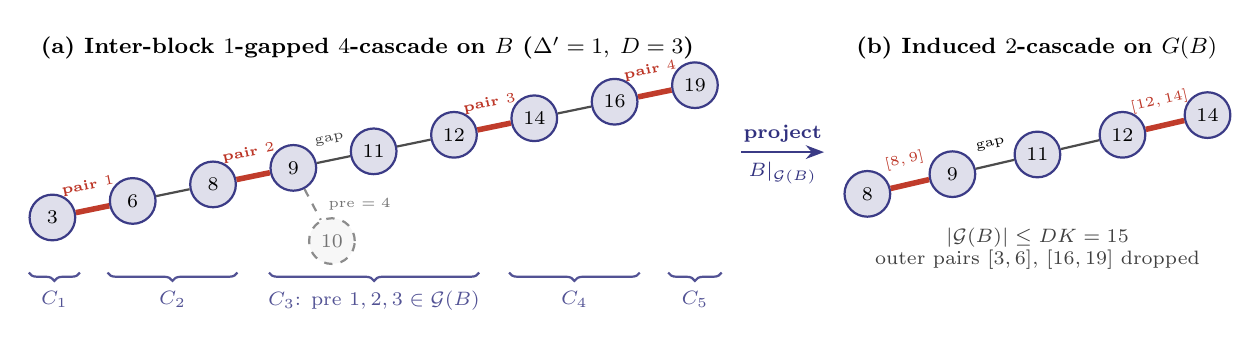
\begin{tikzpicture}[
  >=Stealth,
  cnode/.style={circle, draw=black!80, thick, minimum size=16.5pt, inner sep=0.5pt, font=\scriptsize, fill=white},
  gnode/.style={cnode, fill=MidnightBlue!14, draw=MidnightBlue!85},
  dropnode/.style={cnode, dashed, draw=black!45, text=black!55, fill=black!3},
  rotpair/.style={line width=2.0pt, draw=BrickRed!85},
  lpath/.style={thick, draw=black!70},
  blkbox/.style={rounded corners=3pt, draw=MidnightBlue!35, fill=MidnightBlue!4, inner sep=3pt}
]
  % ---------------- Panel (a): Full BST left-child subpath ----------------
  \begin{scope}[xshift=0cm]
    \node[font=\footnotesize\bfseries] at (4.0, 2.50) {(a) Inter-block $1$-gapped $4$-cascade on $B$ ($\Delta'=1,\; D=3$)};

    % Nodes along slanted left-child path from right (top, 19) to left (bottom, 3)
    \node[gnode] (n3)  at (0.00, 0.35) {$3$};
    \node[gnode] (n6)  at (1.02, 0.56) {$6$};
    \node[gnode] (n8)  at (2.04, 0.77) {$8$};
    \node[gnode] (n9)  at (3.06, 0.98) {$9$};
    \node[gnode] (n11) at (4.08, 1.19) {$11$};
    \node[gnode] (n12) at (5.10, 1.40) {$12$};
    \node[gnode] (n14) at (6.12, 1.61) {$14$};
    \node[gnode] (n16) at (7.14, 1.82) {$16$};
    \node[gnode] (n19) at (8.16, 2.03) {$19$};

    % Non-G(B) right child 10 in C_3 (preorder rank 4 > D = 3)
    \node[dropnode] (n10) at (3.55, 0.05) {$10$};
    \draw[thick, dashed, draw=black!45] (n9) -- node[right=2pt, font=\tiny, text=black!55] {pre $=4$} (n10);

    % Left-child path edges + highlighted cascade pairs (sloped clear of circle rims)
    \draw[rotpair] (n6)  -- node[sloped, above=2pt, font=\tiny\bfseries, text=BrickRed!90] {pair $1$} (n3);
    \draw[lpath]   (n8)  -- (n6);
    \draw[rotpair] (n9)  -- node[sloped, above=2pt, font=\tiny\bfseries, text=BrickRed!90] {pair $2$} (n8);
    \draw[lpath]   (n11) -- node[sloped, above=2pt, font=\tiny, text=black!75] {gap} (n9);
    \draw[lpath]   (n12) -- (n11);
    \draw[rotpair] (n14) -- node[sloped, above=2pt, font=\tiny\bfseries, text=BrickRed!90] {pair $3$} (n12);
    \draw[lpath]   (n16) -- (n14);
    \draw[rotpair] (n19) -- node[sloped, above=2pt, font=\tiny\bfseries, text=BrickRed!90] {pair $4$} (n16);

    % Block brackets underneath
    \draw[decorate, decoration={brace, mirror, amplitude=3pt}, MidnightBlue!75, thick] (-0.30, -0.35) -- node[below=3pt, font=\scriptsize] {$C_1$} (0.35, -0.35);
    \draw[decorate, decoration={brace, mirror, amplitude=3pt}, MidnightBlue!75, thick] (0.70, -0.35) -- node[below=3pt, font=\scriptsize] {$C_2$} (2.35, -0.35);
    \draw[decorate, decoration={brace, mirror, amplitude=3pt}, MidnightBlue!75, thick] (2.75, -0.35) -- node[below=3pt, font=\scriptsize] {$C_3$: pre $1,2,3 \in \mathcal{G}(B)$} (5.42, -0.35);
    \draw[decorate, decoration={brace, mirror, amplitude=3pt}, MidnightBlue!75, thick] (5.80, -0.35) -- node[below=3pt, font=\scriptsize] {$C_4$} (7.46, -0.35);
    \draw[decorate, decoration={brace, mirror, amplitude=3pt}, MidnightBlue!75, thick] (7.82, -0.35) -- node[below=3pt, font=\scriptsize] {$C_5$} (8.50, -0.35);
  \end{scope}

  % Projection arrow
  \draw[->, thick, MidnightBlue!85] (8.75, 1.18) -- node[above, font=\scriptsize\bfseries, text=MidnightBlue!90] {project} node[below, font=\scriptsize, text=MidnightBlue!90] {$B|_{\mathcal{G}(B)}$} (9.80, 1.18);

  % ---------------- Panel (b): Projected 2-cascade on G(B) ----------------
  \begin{scope}[xshift=10.25cm]
    \node[font=\footnotesize\bfseries] at (2.25, 2.50) {(b) Induced $2$-cascade on $G(B)$};
    \node[gnode] (g8)  at (0.10, 0.65) {$8$};
    \node[gnode] (g9)  at (1.18, 0.90) {$9$};
    \node[gnode] (g11) at (2.26, 1.15) {$11$};
    \node[gnode] (g12) at (3.34, 1.40) {$12$};
    \node[gnode] (g14) at (4.42, 1.65) {$14$};

    \draw[rotpair] (g9)  -- node[sloped, above=2pt, font=\tiny\bfseries, text=BrickRed!90] {$[8,9]$} (g8);
    \draw[lpath]   (g11) -- node[sloped, above=2pt, font=\tiny] {gap} (g9);
    \draw[lpath]   (g12) -- (g11);
    \draw[rotpair] (g14) -- node[sloped, above=2pt, font=\tiny\bfseries, text=BrickRed!90] {$[12,14]$} (g12);

    \node[font=\scriptsize, text=black!75, align=center] at (2.26, -0.05) {$|\mathcal{G}(B)| \le D K = 15$\\outer pairs $[3,6],\,[16,19]$ dropped};
  \end{scope}
\end{tikzpicture}
\caption{Reducing $(2i)$-cascades to $(2i - 2)$-cascades on the preorder-$D$ summary BST ($D = \Delta' + 2$): (a) in an inter-block $1$-gapped $4$-cascade ($i = 2$), every inner endpoint $x_r = \mathrm{root}(B|_{C_{a_r}})$ and $y_r$ ($\mathrm{pre}_{B|_{C_{b_r}}}(y_r) \le \Delta' + 2 = 3$) belongs to $\mathcal{G}(B)$, while deeper vertices such as $10$ ($\mathrm{pre} = 4$) lie outside $\mathcal{G}(B)$; (b) the inner pairs $[8, 9], [12, 14]$ execute a $1$-gapped $2$-cascade on $G(B) = B|_{\mathcal{G}(B)}$.}
\label{fig:cascade-summary}
\end{figure}

\paragraph{Proof overview.}
Sundar~\cite[Theorem~3]{Sundar1992} bounded $0$-gapped right $(2i)$-cascades ($\Delta' = 0$), but naively pigeonholing a $\Delta'$-gapped $(2i)$-cascade into $0$-gapped cascades loses an exponential $(\Delta' + 1)^{2i}$ factor. To obtain linear dependence on $\Delta' + 1$, we combine Sundar's $(2i)$-cascade block recursion~\cite[Section~2.1]{Sundar1992} with his preorder-$D$ global-tree summary~\cite[Section~4.2, Theorem~8]{Sundar1992} at $D = \Delta' + 2$, streamlined via the Tamari right-reach characterization (Proposition~\ref{prop:right-reach}): because right-rotation reachability is characterized pointwise by the right-reach $R_T(v) := \max V(T_v)$, every right rotation on $B$ advances the $\LCA$-closed preorder-$D$ summary BST $G(B) := B|_{\mathcal{G}(B)}$ via right rotations (Lemma~\ref{lem:preorder-global}, whose $D = 1$ pure-block-root case is proved inline below since Section~\ref{sec:scale-tree} uses only $D = 1$). Boundary-straddling cascades with an intra-block edge decrease a truncated left-depth potential $\min(\ld_{B|_C}(v), D)$ (Lemma~\ref{lem:cascade-potentials}), while purely inter-block $(2i)$-cascades project onto $(2i - 2)$-cascades on $D K$ vertices, proving Theorem~\ref{thm:mod2-cascade} (the general-$D$ proof of Lemma~\ref{lem:preorder-global} and the complete proofs of Lemma~\ref{lem:cascade-potentials} and Theorem~\ref{thm:mod2-cascade} are deferred to Appendix~\ref{app:cascade-proofs}).

\subsection{Right-Reach Characterization and Preorder-\texorpdfstring{$D$}{D} Summary Trees}
\label{subsec:right-reach}

To test whether one BST can reach another using only right rotations, we track how far to the right each vertex's subtree extends. For any BST $T$ on an ordered finite key set and any vertex $v \in V(T)$, write $T_v$ for the subtree of $T$ rooted at $v$ and define its \emph{right-reach} $R_T(v) := \max V(T_v)$ to be the largest key in $v$'s subtree (any two $n$-node BSTs on possibly different ordered key sets are compared by identifying each key set with $\{1, \dots, n\}$ via in-order rank). Every right rotation $[u, v]$ strictly expands $R(u)$ while leaving $R(x)$ unchanged for all $x \ne u$, and the converse holds as well:

\begin{proposition}[Tamari Right-Reach Characterization]
\label{prop:right-reach}
For any integer $n \ge 1$ and any two BSTs $T_1, T_2$ on $\{1, \dots, n\}$, $T_2$ is reachable from $T_1$ by a (possibly empty) sequence of right single rotations if and only if $R_{T_1}(v) \le R_{T_2}(v)$ for every $v \in \{1, \dots, n\}$.
\end{proposition}

\begin{proof}
Any right single rotation $[u, v]$ ($u = \mathrm{left}_T(v)$) replaces $v\big(u(A, M), R\big)$ by $u\big(A, v(M, R)\big)$, strictly increasing $R(u)$ from $\max V(u(A, M)) < v$ to $R_T(v) \ge v$ while leaving $V(T'_x)$ and $R(x)$ unchanged for all $x \ne u$; hence reachability implies $R_{T_1} \le R_{T_2}$ pointwise.

Conversely, suppose $R_{T_1}(v) \le R_{T_2}(v)$ for all $v \in \{1, \dots, n\}$. Because $V(\mathrm{right}_T(x)) = \{x + 1, \dots, R_T(x)\}$ determines the root of any induced interval $[i, j]$ as the smallest $r \in [i, j]$ with $R_T(r) = j$, $R_{T_1} = R_{T_2}$ implies $T_1 = T_2$. If $T_1 \ne T_2$, pick $u$ with $R_{T_1}(u) < R_{T_2}(u)$ and set $v := R_{T_1}(u) + 1 \le R_{T_2}(u) \le n$. Since $V(T_{1, u})$ is a contiguous interval ending at $v - 1$ that cannot contain a proper ancestor of $u$, we have $\LCA_{T_1}(u, v) = v$, so $u \in V(\mathrm{left}_{T_1}(v))$ and $a := \mathrm{left}_{T_1}(v)$ satisfies $R_{T_1}(a) = v - 1 = R_{T_1}(u)$ and hence $a \le u \le v - 1 = R_{T_1}(a)$ (as $u < a$ would force $R_{T_1}(u) < a$). In $T_2$, $u \in [a, R_{T_2}(a)] \subseteq V(T_{2, a})$ gives $R_{T_2}(u) \le R_{T_2}(a)$ and $v \in [u, R_{T_2}(u)] \subseteq V(T_{2, u})$ gives $R_{T_2}(v) \le R_{T_2}(u)$, so $R_{T_1}(v) \le R_{T_2}(v) \le R_{T_2}(u) \le R_{T_2}(a)$. Right-rotating $[a, v]$ on $T_1$ sets $R_{T'_1}(a) = R_{T_1}(v) \in [v, R_{T_2}(a)]$, preserving $R \le R_{T_2}$ pointwise while strictly decreasing $\sum_{x=1}^n (R_{T_2}(x) - R(x)) \ge 0$; induction completes the proof.
\end{proof}

On $\{1, \dots, n\}$, in-order ordering gives $V(\mathrm{right}_T(v)) = \{v + 1, \dots, R_T(v)\}$ (empty when $R_T(v) = v$), so $R_T(v) = v + |V(\mathrm{right}_T(v))|$ for all $v \in \{1, \dots, n\}$. Pointwise comparison $R_{T_1}(v) \le R_{T_2}(v)$ is therefore identical to componentwise comparison of the right-subtree size (bracket) vector characterizing the Tamari right-rotation order~\cite{Tamari1962,FriedmanTamari1967} (specifically~\cite{HuangTamari1972,Pallo1986}, \cite[Section~9]{BjornerWachs1997}, and~\cite[Section~7.2.1.6]{Knuth2011Vol4A}, up to left--right reversal in~\cite{Pallo1986}).

Next, when $\{1, \dots, N\}$ is partitioned into $K$ contiguous key blocks $C_1 < \dots < C_K$, we compress $B$ into a smaller \emph{preorder-$D$ summary BST} $G(B)$ of size at most $D K$ by keeping only the top $D$ vertices of each block's induced subtree $B|_{C_q}$ in preorder: for any non-empty BST $T$ and $w \in V(T)$, write $\mathrm{pre}_T(w) \in \{1, \dots, |V(T)|\}$ for the $1$-indexed preorder rank of $w$ in $T$ (visiting $\mathrm{root}(T)$, then $\mathrm{left}_T(\mathrm{root}(T))$, then $\mathrm{right}_T(\mathrm{root}(T))$). Using Proposition~\ref{prop:right-reach} and Lemma~\ref{lem:projection-stub}, we generalize Sundar's global-tree construction~\cite[Section~4.2, Theorem~8]{Sundar1992} uniformly to all blocks $C_1, \dots, C_K$ (including $C_1$) and arbitrary $D \ge 1$.

\begin{lemma}[Preorder-$D$ Summary BST Simulation]
\label{lem:preorder-global}
Let $B$ be an $N$-node BST on $\{1, \dots, N\}$ partitioned into contiguous key blocks $C_1 < C_2 < \dots < C_K$, and fix an integer $D \ge 1$. Let $\mathcal{G}(B) := \bigcup_{q=1}^K \big\{w \in C_q : \mathrm{pre}_{B|_{C_q}}(w) \le D\big\}$ consist, within each block $C_q$, of the first $\min(D, |C_q|)$ vertices of $B|_{C_q}$ in preorder.
\begin{enumerate}[label=(\arabic*)]
  \item $\mathcal{G}(B)$ is $\LCA$-closed in $B$, so $G(B) := B|_{\mathcal{G}(B)}$ is a well-defined BST of static size $|\mathcal{G}(B)| = \sum_{q=1}^K \min(D, |C_q|) \le D K$.
  \item Let $B'$ be obtained from $B$ by any right single rotation $[u, v]$. Identifying $\mathcal{G}(B)$ and $\mathcal{G}(B')$ with $\{1, \dots, |\mathcal{G}(B)|\}$ by in-order rank, $G(B')$ is reachable from $G(B)$ via zero or more right single rotations. Moreover, if $u$ and $v$ lie in different blocks, then $\mathcal{G}(B') = \mathcal{G}(B)$, and $G(B')$ is obtained from $G(B)$ by the right single rotation $[u, v]$ when $u, v \in \mathcal{G}(B)$ and satisfies $G(B') = G(B)$ when $\{u, v\} \not\subseteq \mathcal{G}(B)$.
\end{enumerate}
\end{lemma}

Because Section~\ref{sec:scale-tree} invokes Lemma~\ref{lem:preorder-global} solely in the pure-block-root case $D = 1$ (Lemma~\ref{lem:b3-quotient}), we verify $D = 1$ here in a few lines and defer the general $D \ge 1$ proof (needed only inside the proof of Theorem~\ref{thm:mod2-cascade}) to Appendix~\ref{app:cascade-proofs}.

\begin{proof}[Proof of the $D = 1$ case (full proof for all $D \ge 1$ in Appendix~\ref{app:cascade-proofs})]
At $D = 1$, $\mathcal{G}(B) = \{\mathrm{root}(B|_{C_q}) : 1 \le q \le K,\; C_q \ne \emptyset\}$ has $|\mathcal{G}(B)| = \sum_{q=1}^K \min(1, |C_q|) \le K$. For~(1), given $g_1 < g_2$ in $\mathcal{G}(B)$ ($g_1 \in C_{q_1}, g_2 \in C_{q_2}$ with $q_1 < q_2$), let $w := \LCA_B(g_1, g_2) \in C_{q^*}$ ($q_1 \le q^* \le q_2$): if $q_1 < q^* < q_2$, then $g_1 < \min C_{q^*} \le w \le \max C_{q^*} < g_2$ with $g_1, g_2 \in V(B_w)$ prevents $w$ from having any proper ancestor in $C_{q^*}$, forcing $w = \mathrm{root}(B|_{C_{q^*}}) \in \mathcal{G}(B)$; if $q^* \in \{q_1, q_2\}$, then $g_1$ or $g_2$ lies in $V(B_w) \cap C_{q^*}$ and is already $\mathrm{root}(B|_{C_{q^*}})$, forcing $w \in \{g_1, g_2\} \subseteq \mathcal{G}(B)$.

For~(2), if $u \in C_{q_1}$ and $v \in C_{q_2}$ with $q_1 < q_2$, Lemma~\ref{lem:projection-stub}(1) gives $B'|_{C_q} = B|_{C_q}$ for every $q$, so $\mathcal{G}(B') = \mathcal{G}(B)$ and applying Lemma~\ref{lem:projection-stub}(1) with $\mathcal{S} = \mathcal{G}(B)$ gives the inter-block claim ($0$ or $1$ right rotation on $G(B)$). If $u, v \in C_q$ ($u = \mathrm{left}_B(v)$, replacing $B_v = v(u(\widehat{A}, \widehat{M}), \widehat{R})$ with $B'_u = u(\widehat{A}, v(\widehat{M}, \widehat{R}))$), then $B'|_{C_{q'}} = B|_{C_{q'}}$ for $q' \ne q$ and $V(\widehat{M}) \subset (u, v) \subseteq C_q$: if $v \ne \mathrm{root}(B|_{C_q})$, then $\mathrm{root}(B'|_{C_q}) = \mathrm{root}(B|_{C_q})$ so $\mathcal{G}(B') = \mathcal{G}(B)$ with $\{u, v\} \cap \mathcal{G}(B) = \emptyset$ and Lemma~\ref{lem:projection-stub}(1) gives $G(B') = G(B)$; if $v = \mathrm{root}(B|_{C_q})$, then $u = \mathrm{root}(B'|_{C_q})$ gives $\mathcal{G}(B') = (\mathcal{G}(B) \setminus \{v\}) \cup \{u\}$, and $B_v|_{\mathcal{G}(B)} = v(\widehat{A}|_{\mathcal{G}(B)}, \widehat{R}|_{\mathcal{G}(B)})$ and $B'_u|_{\mathcal{G}(B')} = u(\widehat{A}|_{\mathcal{G}(B')}, \widehat{R}|_{\mathcal{G}(B')})$ agree at the identical in-order rank on $\{1, \dots, |\mathcal{G}(B)|\}$, so $G(B') = G(B)$.
\end{proof}


\subsection{Left-Depth Potentials and Recursive Block Contraction for \texorpdfstring{$(2i)$}{(2i)}-Cascades}
\label{subsec:cascade-2i}

Recall from Section~\ref{subsec:overview-mod2} that for $k \ge 1$ and $\Delta' \ge 0$, a \emph{$\Delta'$-gapped right $k$-cascade} on a BST $B$ is a batch of $k$ simultaneous (vertex-disjoint) right single rotations $[x_1, y_1], \dots, [x_k, y_k]$ ($x_1 < y_1 < \dots < x_k < y_k$) along a single left-child subpath $y_k \to \dots \to x_1$ of $B$ ($x_r = \mathrm{left}_B(y_r)$ for each $1 \le r \le k$, with at most $\Delta'$ vertices strictly between $y_r$ and $x_{r+1}$ along that subpath for each $1 \le r < k$), and $C^{\Delta'}_k(N)$ denotes the maximum number of $\Delta'$-gapped right $k$-cascades across any right-rotation sequence on an $N$-node BST. Note first that along any left-child subpath $y_k \to \dots \to x_1$ of $B$, each step down moves from a vertex $w$ to $\mathrm{left}_B(w) < w$, so the vertices on the subpath have keys strictly decreasing from $y_k$ down to $x_1$ (all lying in $[x_1, y_k]$).

\begin{lemma}[Untruncated and Truncated Left-Depth Potentials]
\label{lem:cascade-potentials}
\leavevmode
\begin{enumerate}[label=(\arabic*)]
  \item For any BST $T$, $\Phi_{\ld}(T) := \sum_{v \in V(T)} \ld_T(v) \in \big[0, \binom{|V(T)|}{2}\big]$ decreases by at least~$1$ under every right single rotation on $T$ ($\Delta\Phi_{\ld}(T) \le -1$), so any batch of $k$ simultaneous right single rotations on $T$ satisfies $\Delta\Phi_{\ld}(T) \le -k$.
  \item Fix $D := \Delta' + 2 \ge 2$ and contiguous key blocks $C_1 < \dots < C_K$ partitioning $\{1, \dots, N\}$. For each block $C = C_q$, define
  \[
  \Psi_C(B) \;:=\; |\LS(B|_C)| + \sum_{v \in C} \min\big(\ld_{B|_C}(v),\, D\big) \;\in\; \big[0,\, (D + 1)|C|\big].
  \]
  Then $\Psi_C(B)$ is non-increasing under every right single rotation on $B$, and every $\Delta'$-gapped right $k$-cascade ($k \ge 2$) on $B$ with $x_1 \in C_{q_{\min}}$, $y_k \in C_{q_{\max}}$ ($q_{\min} < q_{\max}$), and at least one intra-block edge $[x_r, y_r] \subseteq C_q$ decreases $\sum_{q=1}^K \Psi_{C_q}(B)$ by at least~$1$.
\end{enumerate}
\end{lemma}

With Lemmas~\ref{lem:preorder-global} and~\ref{lem:cascade-potentials} in hand at $D = \Delta' + 2$, the proof of Theorem~\ref{thm:mod2-cascade} in Appendix~\ref{app:cascade-proofs} bounds $C^{\Delta'}_2(N)$ for general $N \ge 1$ by iterated bisection against $\Phi_{\ld}$ and $\Psi_C$, defines pure-integer block thresholds $M^{(D)}_i(j) = D\,\mu_i(j) \ge 12 D\,A_i(j)$ ($i \ge 2, j \ge 1$), proves $C^{\Delta'}_{2i}\big(M^{(D)}_i(j)\big) \le 3(D + 1)\,j\,M^{(D)}_i(j)$ by two-parameter induction on $(i, j)$ (recursing intra-block cascades at $(i, j - 1)$, discharging mixed boundary-straddling cascades via $\Psi_C$, and projecting purely inter-block $(2i)$-cascades onto $(2i - 2)$-cascades on $G(B)$ of size $D K$), and chains $\lfloor M^{(D)}_i(1) / N \rfloor$ copies of an $N$-node BST along a right spine for $1 \le N \le A_i(1)$ to obtain $C^{\Delta'}_{2i}(N) \le 18(\Delta' + 1)\,N$ ($C_{\mathrm{casc}} := 18$).


% ============================================================================
\section{Scale-Tree Self-Reduction of a Folded \texorpdfstring{$\POP$}{Pop} Process}
\label{sec:scale-tree}
% ============================================================================

\subsection{Valid Scale Trees and the Contraction-Pass Reduction}
\label{subsec:overview-mod3}

Our next reduction acts entirely on folded $\POP$ processes. To amortize across $M$ nested partitions $\mathcal{P}_0 \succ \mathcal{P}_1 \succ \dots \succ \mathcal{P}_M$ of $\{1, \dots, P\}$ at once without letting scale weights blow up, we organize the scales $\{1, \dots, M\}$ as the leaves of a rooted \emph{scale tree} $\mathcal{T}$ of height at most $r$. Given \emph{any} valid scale tree $\mathcal{T}$ of height at most $r$, a single multi-scale amortization pass self-reduces a size-$P$ folded $\POP$ process $\widetilde{H}$ to independent leaf folded $\POP$ processes $\{\widetilde{H}^{(Q)}\}_{Q \in \mathcal{P}_M}$ at $+C_{\mathrm{pass}}\,r\,P$ additive cost, with a universal constant $C_{\mathrm{pass}}$ independent of $P, r, M$, and $\mathcal{T}$. This decouples the dynamic BST analysis from the purely arithmetic task of constructing valid scale trees (Section~\ref{sec:contraction}).

\begin{definition}[Scale Tree and Nested Block Partitions]
\label{def:scale-tree}
Fix integers $P \ge 1$, $r \ge 1$, and $M \ge 1$.
\begin{enumerate}[label=(\arabic*), leftmargin=2em, itemsep=2pt]
  \item \emph{Scale tree $\mathcal{T}$ and path weights $w(\xi)$.} A \emph{scale tree of height at most $r$} on scales $\{1, \dots, M\}$ is a rooted ordered tree $\mathcal{T}$ whose leaves in left-to-right order are the partition scales $\{1, \dots, M\}$ (distinct from the keys $\{1, \dots, P\}$), each at depth $\delta(\ell) \in \{1, \dots, r\}$. To keep the reciprocal leaf weights summable ($\sum_{\ell=1}^M w_\ell^{-1} < \frac{1}{2}$) while resetting child counters inside every subtree, the edge from any internal node to its $c$-th child ($c \ge 1$) carries multiplier $4 c^2$; each node $\xi \in \mathcal{T}$ with child indices $c_1, \dots, c_{\delta(\xi)} \ge 1$ along the root-to-$\xi$ path then has path weight $w(\xi) := \prod_{q=1}^{\delta(\xi)} (4 c_q^2)$ (setting $w(\mathrm{root}) := 1$ and writing $w_\ell := w(\ell)$ for leaves $\ell \in \{1, \dots, M\}$).
  \item \emph{Valid nested block partitions $\mathcal{P}_0 \succ \dots \succ \mathcal{P}_M$.} Setting $S_0 := P$ and starting from the single-block partition $\mathcal{P}_0 := \{\{1, \dots, P\}\}$, we say $\mathcal{T}$ \emph{validly partitions} $\{1, \dots, P\}$ if at each scale $\ell = 1, \dots, M$---setting $i_\ell$ to the Ackermann level covering parent blocks of size $< 2 S_{\ell-1}$, and sizing sub-blocks by $w_\ell i_\ell^2$ to absorb $O(i_\ell^2)$ cascade overhead per sub-block---the target block size $S_\ell$ shrinks by at least half according to
  \[
  i_\ell \;:=\; \alpha_0(2 S_{\ell-1}) + 1, \qquad
  S_\ell \;:=\; w_\ell\,i_\ell^2 \;\le\; \frac{1}{2} S_{\ell-1},
  \]
  and $\mathcal{P}_0 \succ \mathcal{P}_1 \succ \dots \succ \mathcal{P}_M$ is the chain of nested contiguous-interval partitions obtained by splitting each parent block $X \in \mathcal{P}_{\ell-1}$ (which inductively satisfies $|X| \in [S_{\ell-1}, 2 S_{\ell-1})$) from left to right into $K_X := \lfloor |X| / S_\ell \rfloor \ge 2$ contiguous sub-blocks, where the first $K_X - 1$ sub-blocks have exact size $S_\ell$ and the last sub-block absorbs the remainder $|X| - (K_X - 1) S_\ell \in [S_\ell, 2 S_\ell)$.
\end{enumerate}
Note that $1 \le K_X - 1 < K_X < 2 S_{\ell-1} \le A_{i_\ell - 1}(1) < A_{i_\ell}(1)$, directly matching the hypothesis $N \le A_i(1)$ of Theorem~\ref{thm:mod2-cascade} at $N = K_X - 1$ and $i = i_\ell$.
\end{definition}

\begin{theorem}[Scale-Tree Contraction Pass and Bisection Bound]
\label{thm:mod3-pass}
There exists an absolute constant $C_{\mathrm{pass}} > 0$ (independent of $P, r, M$, and $\mathcal{T}$) such that for every folded $\POP$ process $\widetilde{H}$ of size $P \ge 1$:
\begin{enumerate}[label=(\arabic*)]
  \item For every integer $r \ge 1$ and every scale tree $\mathcal{T}$ of height at most $r$ on $M \ge 1$ scales that validly partitions $\{1, \dots, P\}$, there exist folded $\POP$ processes $\{\widetilde{H}^{(Q)}\}_{Q \in \mathcal{P}_M}$ of sizes $1 \le |Q| < 2 S_M$ with $\sum_{Q \in \mathcal{P}_M} |Q| = P$ such that
  \[
  J(\widetilde{H}) \;\le\; C_{\mathrm{pass}}\,r\,P \;+\; \sum_{Q \in \mathcal{P}_M} J(\widetilde{H}^{(Q)}).
  \]
  \item \emph{(Elementary bisection bound)} For all $P \ge 1$, $J(\widetilde{H}) \le P \max\big(0, \lceil \log_2 P \rceil - 1\big)$.
\end{enumerate}
\end{theorem}

\paragraph{Example (variable-depth valid scale tree at $P = 3{,}200$ and four-way rotation routing).}
Even at $P = 3{,}200$ (where $2 S_0 = 6{,}400 \in (A_3(1), A_4(1)]$ gives $i_1 = \alpha_0(6{,}400) + 1 = 5$), the height-$3$ variable-depth tree $\mathcal{T}$ on $M = 2$ scales placing leaf $\ell = 1$ at depth~$3$ along $c = (1, 1, 1)$ ($w_1 = 4^3 = 64$) and leaf $\ell = 2$ at depth~$1$ along $c = (2)$ ($w_2 = 4 \cdot 2^2 = 16$, with $w_1^{-1} + w_2^{-1} = \frac{5}{64} < \frac{1}{2}$) validly partitions $\{1, \dots, 3{,}200\}$: scale~$1$ has $S_1 = 64 \cdot 5^2 = 1{,}600 \le \frac{1}{2} S_0$, and scale~$2$ has $i_2 = \alpha_0(3{,}200) + 1 = 5$ and $S_2 = 16 \cdot 5^2 = 400 \le \frac{1}{2} S_1 = 800$, decomposing $\widetilde{H}$ into eight $400$-key leaf processes $\widetilde{H}^{(Q)}$. Figure~\ref{fig:scale-tree-routing} illustrates $\LCA_{\mathcal{T}}$ routing on a general scale tree alongside the four-way classification of an internal $\POP(s)$ rotation $e = (x, y, z)$ ($s < x < y < z$) by comparing $\sep(s, x)$ against $\ell = \sep(x, y)$.

\begin{figure}[ht]
\centering
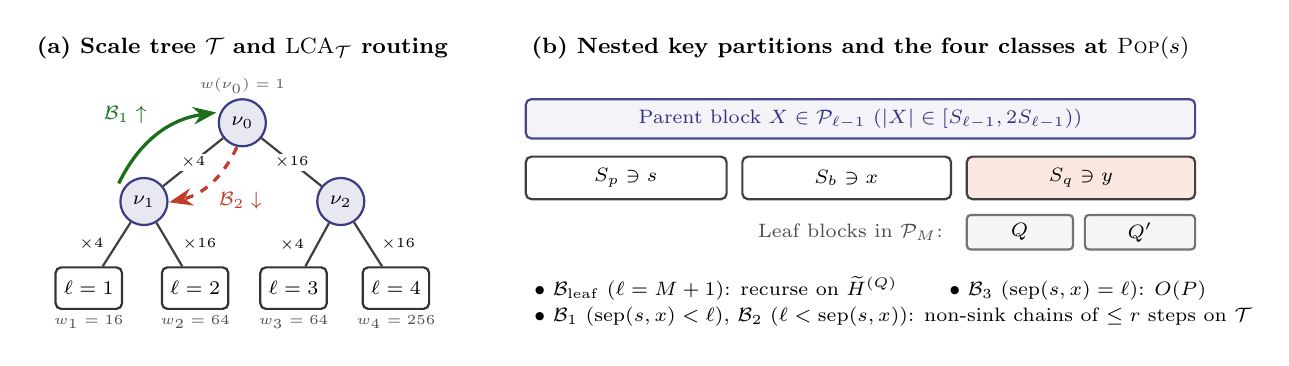
\begin{tikzpicture}[
  >=Stealth,
  tnode/.style={circle, draw=MidnightBlue!85, fill=MidnightBlue!10, thick, minimum size=17pt, inner sep=1pt, font=\scriptsize},
  lnode/.style={rectangle, rounded corners=2pt, draw=black!80, fill=white, thick, minimum width=24pt, minimum height=15pt, inner sep=1.5pt, font=\scriptsize},
  tedge/.style={thick, draw=black!75}
]
  % ---------------- Panel (a): Scale tree and LCA routing ----------------
  \begin{scope}[xshift=0cm]
    \node[font=\footnotesize\bfseries] at (2.25, 3.30) {(a) Scale tree $\mathcal{T}$ and $\LCA_{\mathcal{T}}$ routing};

    \node[tnode] (r0) at (2.25, 2.35) {$\nu_0$};
    \node[font=\tiny, text=black!65] at (2.25, 2.82) {$w(\nu_0) = 1$};

    \node[tnode] (r1) at (1.00, 1.35) {$\nu_1$};
    \node[tnode] (r2) at (3.50, 1.35) {$\nu_2$};

    \node[lnode] (l1) at (0.30, 0.25) {$\ell=1$};
    \node[lnode] (l2) at (1.65, 0.25) {$\ell=2$};
    \node[lnode] (l3) at (2.90, 0.25) {$\ell=3$};
    \node[lnode] (l4) at (4.20, 0.25) {$\ell=4$};

    \node[font=\tiny, text=black!70] at (0.30, -0.18) {$w_1=16$};
    \node[font=\tiny, text=black!70] at (1.65, -0.18) {$w_2=64$};
    \node[font=\tiny, text=black!70] at (2.90, -0.18) {$w_3=64$};
    \node[font=\tiny, text=black!70] at (4.20, -0.18) {$w_4=256$};

    \draw[tedge] (r0) -- node[pos=0.50, fill=white, inner sep=1pt, font=\tiny] {$\times 4$} (r1);
    \draw[tedge] (r0) -- node[pos=0.50, fill=white, inner sep=1pt, font=\tiny] {$\times 16$} (r2);
    \draw[tedge] (r1) -- node[left=1pt, font=\tiny] {$\times 4$} (l1);
    \draw[tedge] (r1) -- node[right=1pt, font=\tiny] {$\times 16$} (l2);
    \draw[tedge] (r2) -- node[left=1pt, font=\tiny] {$\times 4$} (l3);
    \draw[tedge] (r2) -- node[right=1pt, font=\tiny] {$\times 16$} (l4);

    % Upward B1 arrow and downward B2 arrow (into non-rightmost child \nu_1)
    \draw[->, very thick, ForestGreen!80!black] (0.68, 1.58) to[bend left=28] node[above left=0pt, font=\scriptsize\bfseries, text=ForestGreen!80!black] {$\mathcal{B}_1 \uparrow$} (1.92, 2.48);
    \draw[->, very thick, BrickRed!85, dashed] (2.18, 2.04) to[bend left=26] node[below right=-1pt, font=\scriptsize\bfseries, text=BrickRed!85] {$\mathcal{B}_2 \downarrow$} (1.32, 1.34);
  \end{scope}

  % ---------------- Panel (b): Nested key blocks and 4 classes ----------------
  \begin{scope}[xshift=5.65cm]
    \node[font=\footnotesize\bfseries] at (4.45, 3.30) {(b) Nested key partitions and the four classes at $\POP(s)$};

    % Coarse block X in P_{l-1}
    \draw[thick, rounded corners=2pt, draw=MidnightBlue!80, fill=MidnightBlue!5] (0.20, 2.15) rectangle (8.70, 2.65);
    \node[font=\scriptsize, text=MidnightBlue!90] at (4.45, 2.40) {Parent block $X \in \mathcal{P}_{\ell-1}$ ($|X| \in [S_{\ell-1}, 2S_{\ell-1})$)};

    % Three child sub-blocks S_p < S_b < S_q in P_l
    \draw[thick, rounded corners=2pt, draw=black!75, fill=white] (0.20, 1.38) rectangle (2.75, 1.92);
    \draw[thick, rounded corners=2pt, draw=black!75, fill=white] (2.95, 1.38) rectangle (5.60, 1.92);
    \draw[thick, rounded corners=2pt, draw=black!75, fill=BrickRed!8] (5.80, 1.38) rectangle (8.70, 1.92);

    \node[font=\scriptsize] at (1.47, 1.65) {$S_p \ni s$};
    \node[font=\scriptsize] at (4.27, 1.65) {$S_b \ni x$};
    \node[font=\scriptsize] at (7.25, 1.65) {$S_q \ni y$};

    % Leaf blocks Q in P_M
    \node[font=\scriptsize, text=black!70, anchor=east] at (5.62, 0.96) {Leaf blocks in $\mathcal{P}_M$:};
    \draw[thick, rounded corners=1.5pt, draw=black!55, fill=black!4] (5.80, 0.74) rectangle (7.15, 1.18);
    \draw[thick, rounded corners=1.5pt, draw=black!55, fill=black!4] (7.30, 0.74) rectangle (8.70, 1.18);
    \node[font=\scriptsize] at (6.47, 0.96) {$Q$};
    \node[font=\scriptsize] at (8.00, 0.96) {$Q'$};

    % Two-line legend of 4 classes at bottom (fits strictly inside [0.20, 8.70])
    \node[font=\scriptsize, align=left, anchor=north west] at (0.18, 0.52) {%
      $\bullet$ $\mathcal{B}_{\mathrm{leaf}}$ ($\ell = M+1$): recurse on $\widetilde{H}^{(Q)}$ \qquad
      $\bullet$ $\mathcal{B}_3$ ($\sep(s,x)=\ell$): $O(P)$\\[1.5pt]
      $\bullet$ $\mathcal{B}_1$ ($\sep(s,x)<\ell$), $\mathcal{B}_2$ ($\ell<\sep(s,x)$): non-sink chains of $\le r$ steps on $\mathcal{T}$};
  \end{scope}
\end{tikzpicture}
\caption{Simultaneous multi-scale amortization on a height-$r$ scale tree $\mathcal{T}$: (a) edge factors $4c^2$ reset to $\times 4, \times 16, \dots$ inside each fresh subtree while keeping $\sum_\ell w_\ell^{-1} < \frac{1}{2}$, and non-sink split-scale cascade chains move $\nu(e) = \LCA_{\mathcal{T}}(\sep(s,x), \ell)$ strictly up $\mathcal{T}$ in $\mathcal{B}_1$ and strictly down $\mathcal{T}$ in $\mathcal{B}_2$; (b) same-scale rotations $\mathcal{B}_3$ place $s < x < y$ in three sibling sub-blocks $S_p < S_b < S_q$ of $X \in \mathcal{P}_{\ell-1}$ and are bounded in $O(P)$ independently of $r$ and $M$.}
\label{fig:scale-tree-routing}
\end{figure}

\paragraph{Proof overview.}
For $u < v$ in $\{1, \dots, P\}$, let $\sep(u, v) \in \{1, \dots, M + 1\}$ be the smallest $\ell \le M$ putting $u$ and $v$ in different blocks of $\mathcal{P}_\ell$ (or $M + 1$ if $u, v$ share a leaf block $Q \in \mathcal{P}_M$). Partition $\mathcal{R}_{\mathrm{int}}(\widetilde{H})$ at $\POP(s)$ ($s < x < y < z$, $\ell := \sep(x, y)$) into four classes by comparing the trigger scale $\sep(s, x)$ against $\ell$, bounded along an acyclic chain of $O(P)$ estimates whose implied constants are all independent of $r, M$, and $\mathcal{T}$:
\begin{itemize}[leftmargin=2em]
  \item \emph{Intra-leaf rotations ($\mathcal{B}_{\mathrm{leaf}}$, $\ell = M + 1$):} $x, y \in Q \in \mathcal{P}_M$. Pre-activation rotations ($s < \min Q$) freeze $y$ until $\POP(x)$ with $x \in Q$ ($\le P$), exit rotations ($z > \max Q$) occur at most once per $\POP$ ($\le P$), and active rotations ($s, x, y, z \in Q$) project onto independent folded $\POP$ processes $\widetilde{H}^{(Q)}$.
  \item \emph{Split-scale rotations---coarse-trigger ($\mathcal{B}_1$, $\sep(s, x) < \ell \le M$) and fine-trigger ($\mathcal{B}_2$, $\ell < \sep(s, x)$):} Route $e$ to $\nu(e) = \LCA_{\mathcal{T}}(\sep(s, x), \ell) \in \mathcal{T}_{\mathrm{int}}$. Along consecutive pairs $e \to e^+$ in the same $\POP$ cascade, unless $e$ freezes a block at a subtree's finest scale (summing to $\Sigma_{\mathcal{T}} = O(P)$ via $\sum_{\nu \in \mathcal{T}_{\mathrm{int}}} w(\nu)^{-1} < 2$, so the sink set $\mathcal{S}_1$ satisfies $|\mathcal{S}_1| = O(P)$) or is topmost ($\le P$), $\nu(e^+)$ is a \emph{strict ancestor} of $\nu(e)$ in $\mathcal{B}_1$ and a \emph{strict descendant} of $\nu(e)$ in $\mathcal{B}_2$ (or exits $\mathcal{B}_2$ into $\mathcal{B}_1 \sqcup \mathcal{B}_3$). Cascade-path sink counting between $\mathcal{B}_1$ and $\mathcal{B}_1 \setminus \mathcal{S}_1$ bounds external entries into $\mathcal{B}_1$ by $|\mathcal{E}_{\mathrm{enter}}| \le |\mathcal{S}_1| + |\mathcal{B}_{\mathrm{leaf, pre}}| = O(P)$ \emph{independently of $r$ and $M$}.
  \item \emph{Same-scale (three-block) rotations ($\mathcal{B}_3$, $\sep(s, x) = \ell \le M$, so $s \in S_p < S_b \ni x < S_q \ni y$ inside $X \in \mathcal{P}_{\ell-1}$):} Bounded in $O(P)$ \emph{independently of $r$ and $M$}:
    \begin{enumerate}[label=(\roman*)]
      \item \emph{Intra-block ($z \in S_q$):} A two-step parent-confinement potential $\Phi_{\mathrm{conf}}$ on the first-child/right-sibling tree $L''$ of $\widetilde{H}$, paired with $|\mathcal{E}_{\mathrm{enter}}| = O(P)$, bounds $|\mathcal{B}_{3,\mathrm{intra}}| = O(P)$.
      \item \emph{Post-depletion exits ($z > \max S_q$ after keys initially in $S_p$ are gone):} A block-descendant potential $\Psi_{\mathrm{post}}$ on the unfolded BST bounds $|\mathcal{B}_{3,\mathrm{exit, post}}| \le K_L < 2P$.
      \item \emph{Active exits ($z > \max S_q$ while $S_p$ still holds pre-existing keys):} Because parent keys in $\widetilde{H}$ only increase under right rotations, each promoted key $x$ can serve as the promoted key in $\mathcal{B}_{3,\mathrm{exit}}$ at \emph{at most one scale $\ell$} across the entire execution. Monotone parent-crossing injectivity charges secondary exits $A_{\mathrm{esc}}$ and gap-witness sets $\sum_{\ell=1}^M |U_\ell|$ in $O(P)$ to base, $\mathcal{B}_{3,\mathrm{intra}}$, and $\mathcal{S}_1$ events; embedding future keys into the insertion-time Cartesian extension $\widetilde{H}^*$ turns lead exits ($\Delta_\ell = i_\ell$, $\Delta'_\ell = 2 i_\ell$) into $(2 i_\ell)$-cascades on a $(K_X - 1)$-node pure-right-rotation block-root summary BST $\widehat{G}_X$, where Theorem~\ref{thm:mod2-cascade} ($N = K_X - 1 \le A_{i_\ell}(1)$) and $\sum_{\ell=1}^M w_\ell^{-1} < \frac{1}{2}$ bound $\sum |\widetilde{\mathcal{N}}_p^{(\ell)}| = O(P)$ and hence $|\mathcal{B}_3| = O(P)$, closing $|\mathcal{B}_2| = O(r P)$.
    \end{enumerate}
\end{itemize}

Beyond basic interval properties of nested key partitions, the proof below depends only on BST interval projection and emptying initialization (Lemmas~\ref{lem:projection-stub} and~\ref{lem:emptying-sim}), the three structural laws of $\widetilde{H}$ (Lemma~\ref{lem:folded-laws}), and the right-reach characterization, preorder-$1$ summary BST simulation, and bounded-gap cascade bound of Section~\ref{sec:cascades} (Proposition~\ref{prop:right-reach}, Lemma~\ref{lem:preorder-global}, and Theorem~\ref{thm:mod2-cascade}).

\subsection{Convergent Leaf and Internal Weights on Height-\texorpdfstring{$r$}{r} Scale Trees}
\label{subsec:tree-weights}

Let $\mathcal{T}$ be a scale tree of height at most $r$ on scales $\{1, \dots, M\}$ that validly partitions $\{1, \dots, P\}$ (Definition~\ref{def:scale-tree}), and let $\mathcal{T}_{\mathrm{int}}$ denote the set of internal nodes of $\mathcal{T}$. Every internal node $\nu \in \mathcal{T}_{\mathrm{int}}$ sits at depth $\delta(\nu) \in \{0, \dots, r - 1\}$ from $\mathrm{root}(\mathcal{T})$ and has $k_\nu \ge 1$ ordered children $\nu_1, \dots, \nu_{k_\nu}$ whose leaf subtrees partition the contiguous scale interval of $\nu$ into consecutive child intervals $(m_0, m_1], (m_1, m_2], \dots, (m_{k_\nu - 1}, m_{k_\nu}]$, where we write $M_{\mathrm{end}}(\nu) := m_{k_\nu}$ for the rightmost (finest) scale in $\nu$'s subtree:
\[
\begin{array}{c}
\nu = \LCA_{\mathcal{T}}(\ell_1, \ell_2) \;\; \big(\text{path weight } w(\nu),\; \delta(\nu) \in \{0, \dots, r - 1\}\big)\\[4pt]
\swarrow \text{\scriptsize $\times 4 c_1^2$} \qquad\qquad \downarrow \text{\scriptsize $\times 4 c_2^2$} \qquad\qquad \searrow \text{\scriptsize $\times 4 k_\nu^2$}\\[4pt]
\underbrace{(m_{c_1 - 1}, m_{c_1}]}_{\ni\, \ell_1}
\quad < \quad
\underbrace{(m_{c_2 - 1}, m_{c_2}]}_{\ni\, \ell_2}
\quad \le \quad
\underbrace{(m_{k_\nu - 1}, m_{k_\nu}]}_{\text{rightmost leaf } m_{k_\nu} = M_{\mathrm{end}}(\nu)}
\end{array}
\]

Notice first that valid partitioning enforces a uniform numerical floor at every scale $\ell \in \{1, \dots, M\}$: since $\delta(\ell) \ge 1$, every leaf has $w_\ell \ge 4$; since $S_{\ell-1} \ge 1$, Definition~\ref{def:ackermann} gives $i_\ell = \alpha_0(2 S_{\ell-1}) + 1 \ge 2$, whence $S_\ell = w_\ell i_\ell^2 \ge 16$ and $S_{\ell-1} \ge 2 S_\ell \ge 32$. Thus $2 S_{\ell-1} \ge 64 > 16 = A_3(1)$, so $\alpha_0(2 S_{\ell-1}) \ge 4$ and therefore
\begin{equation}
\label{eq:scale-floor}
i_\ell \;\ge\; 5, \qquad S_\ell \;=\; w_\ell\,i_\ell^2 \;\ge\; 25\,w_\ell \;\ge\; 100, \qquad\text{and}\qquad S_{\ell-1} \;\ge\; 2 S_\ell \;\ge\; 200 \qquad (1 \le \ell \le M).
\end{equation}

\begin{lemma}[Height-Independent Weight Convergence]
\label{lem:tree-weights}
For every integer $r \ge 1$ and every scale tree $\mathcal{T}$ of height at most $r$ on $M \ge 1$ scales that validly partitions $\{1, \dots, P\}$, we have
\[
\sum_{\ell=1}^M \frac{1}{w_\ell} \;<\; \frac{1}{2},
\qquad
\sum_{\nu \in \mathcal{T}_{\mathrm{int}}} \frac{1}{w(\nu)} \;<\; 2,
\qquad\text{and}\qquad
\Sigma_{\mathcal{T}} \;:=\; \sum_{\nu \in \mathcal{T}_{\mathrm{int}}} k_\nu\,\big|\mathcal{P}_{M_{\mathrm{end}}(\nu)}\big| \;<\; \frac{P}{50}.
\]
\end{lemma}

\begin{proof}
Observe that $\sum_{c=1}^\infty \frac{1}{4 c^2} = \frac{\pi^2}{24} < \frac{1}{2}$. For any node $\xi \in \mathcal{T}$ of subtree height $q \ge 0$ (the maximum edge distance from $\xi$ to a leaf in $\mathcal{T}_\xi$), induction on $q$ gives $\sum_{\ell \in \mathrm{Leaves}(\mathcal{T}_\xi)} \big(w_\ell / w(\xi)\big)^{-1} \le 1$, with strict bound $\le \sum_{c=1}^{k_\xi} \frac{1}{4 c^2} \cdot 1 < \frac{1}{2}$ whenever $q \ge 1$; setting $\xi = \mathrm{root}(\mathcal{T})$ ($w(\xi) = 1$, $q \ge 1$) yields $\sum_{\ell=1}^M w_\ell^{-1} < \frac{1}{2}$. Likewise, at each depth $\delta \in \{0, \dots, r - 1\}$, summing $w(\nu)^{-1}$ over all nodes $\nu \in \mathcal{T}_{\mathrm{int}}$ with $\delta(\nu) = \delta$ is at most $\big(\sum_{c=1}^\infty \frac{1}{4 c^2}\big)^\delta \le 2^{-\delta}$, so $\sum_{\nu \in \mathcal{T}_{\mathrm{int}}} w(\nu)^{-1} \le \sum_{\delta=0}^{r-1} 2^{-\delta} < 2$.

Finally, fix $\nu \in \mathcal{T}_{\mathrm{int}}$ and set $\ell^* := M_{\mathrm{end}}(\nu)$. The root-to-$\ell^*$ path in $\mathcal{T}$ traverses the edge from $\nu$ to its $k_\nu$-th child (factor $4 k_\nu^2$) followed by zero or more edges of factor $\ge 4 \ge 1$, so $w_{\ell^*} \ge 4 k_\nu^2\,w(\nu)$. By~\eqref{eq:scale-floor}, $i_{\ell^*} \ge 5$, giving $S_{\ell^*} = w_{\ell^*} i_{\ell^*}^2 \ge 100\,k_\nu^2\,w(\nu)$. Since every block in $\mathcal{P}_{\ell^*}$ has size at least $S_{\ell^*}$, we have $|\mathcal{P}_{\ell^*}| \le P / S_{\ell^*}$ and hence
\[
k_\nu\,\big|\mathcal{P}_{M_{\mathrm{end}}(\nu)}\big| \;\le\; \frac{k_\nu\,P}{100\,k_\nu^2\,w(\nu)} \;\le\; \frac{P}{100\,w(\nu)}.
\]
Summing over $\nu \in \mathcal{T}_{\mathrm{int}}$ via $\sum_{\nu \in \mathcal{T}_{\mathrm{int}}} w(\nu)^{-1} < 2$ gives $\Sigma_{\mathcal{T}} < \frac{2P}{100} = \frac{P}{50}$.
\end{proof}


\subsection{Separating Scales, Rotation Classification, and Leaf Subprocess Projection}
\label{subsec:bucket-defs}

To amortize internal $\POP$ rotations across a hierarchy of nested key partitions $\mathcal{P}_0 \succ \mathcal{P}_1 \succ \dots \succ \mathcal{P}_M$ of $\{1, \dots, P\}$, we assign every pair of keys the first scale at which they split into different blocks, and then sort each internal $\POP(s)$ rotation $e = (x, y, z)$ ($s < x < y < z$) according to whether the deleted key $s$ separates from $x$ at a coarser, finer, or identical scale compared to where $x$ separates from $y$. No numerical condition on block sizes is needed for this classification or for Lemma~\ref{lem:bucket-leaf}, allowing Theorem~\ref{thm:mod3-pass}(2) and Section~\ref{sec:frontiers} to invoke them directly on bisection and dyadic partitions.

\begin{definition*}[Separating Scale and Four-Way Rotation Classification]
Let $\widetilde{H}$ be a folded $\POP$ process of size $P \ge 1$, and let $\mathcal{P}_0 \succ \mathcal{P}_1 \succ \dots \succ \mathcal{P}_M$ ($M \ge 1$) be any nested chain of contiguous-interval partitions of $\{1, \dots, P\}$ starting from $\mathcal{P}_0 = \{\{1, \dots, P\}\}$. For $u \in \{1, \dots, P\}$ and $0 \le \ell \le M$, let $B_\ell(u) \in \mathcal{P}_\ell$ denote the unique block of $\mathcal{P}_\ell$ containing $u$; for a block $Q \in \mathcal{P}_{\ell'}$ at a finer level $\ell' \ge \ell$, write $B_\ell(Q) := B_\ell(\min Q)$ for its enclosing block in $\mathcal{P}_\ell$.
\begin{enumerate}[label=(\arabic*), leftmargin=2em, itemsep=3pt]
  \item \emph{Separating scale $\sep(u, v)$.} Zooming in from the single coarse block $\mathcal{P}_0 = \{\{1, \dots, P\}\}$ down to the leaf blocks $\mathcal{P}_M$, the \emph{separating scale} $\sep(u, v) \in \{1, \dots, M + 1\}$ of $u, v \in \{1, \dots, P\}$ is the first (coarsest) scale $\ell$ at which $u$ and $v$ fall into different blocks (or $M + 1$ if they remain in the same leaf block of $\mathcal{P}_M$):
  \[
  \sep(u, v) \;:=\;
  \begin{cases}
  M + 1 & \text{if } B_M(u) = B_M(v),\\
  \min\big\{\ell \in \{1, \dots, M\} : B_\ell(u) \ne B_\ell(v)\big\} & \text{otherwise.}
  \end{cases}
  \]
  Smaller values of $\sep(u, v)$ mean $u$ and $v$ split apart at a \emph{coarser} scale, whereas larger values mean they stay together down to a \emph{finer} scale; whenever $\sep(u, v) = \ell \in \{1, \dots, M\}$, they share a parent block $B_{\ell-1}(u) = B_{\ell-1}(v)$ and lie in distinct scale-$\ell$ sub-blocks $B_\ell(u) \ne B_\ell(v)$.
  \item \emph{Four-way rotation classification.} Every internal $\POP$ rotation $e = (x, y, z) = (v_{2j-1}, v_{2j}, v_{2j+1}) \in \mathcal{R}_{\mathrm{int}}(\widetilde{H})$ ($1 \le j \le h$) during $\POP(s)$ satisfies $s < x < y < z$, rotating the \emph{promoted key} $x$ above the \emph{displaced key} $y$ directly below $y$'s old spine parent $z$ (which becomes $x$'s new spine parent). Comparing the \emph{trigger scale} $\sep(s, x)$ against the \emph{rotation scale} $\ell := \sep(x, y) \in \{1, \dots, M + 1\}$ partitions $\mathcal{R}_{\mathrm{int}}(\widetilde{H}) = \mathcal{B}_{\mathrm{leaf}} \sqcup \mathcal{B}_1 \sqcup \mathcal{B}_2 \sqcup \mathcal{B}_3$ into four disjoint classes:
  \begin{itemize}[leftmargin=1.6em, itemsep=2pt, topsep=2pt]
    \item \emph{Intra-leaf rotations} $\mathcal{B}_{\mathrm{leaf}}$ ($\ell = M + 1$): $x$ and $y$ lie in the \emph{same leaf block} $Q \in \mathcal{P}_M$, split further according to whether $Q$ has begun deleting and whether $z$ stays inside $Q$:
    \begin{itemize}[leftmargin=1.4em, itemsep=1pt, topsep=1pt]
      \item $\mathcal{B}_{\mathrm{leaf,pre}}$ (\emph{pre-activation}, $s < \min Q$): triggered by a deletion in an earlier block before any key of $Q$ is popped;
      \item $\mathcal{B}_{\mathrm{leaf,exit}}$ (\emph{leaf-exit}, $s \in Q$ and $z > \max Q$): triggered inside $Q$, but $x$'s new parent $z$ lies strictly outside $Q$;
      \item $\mathcal{B}_{\mathrm{leaf,act}}$ (\emph{active intra-leaf}, $s, x, y, z \in Q$): triggered inside $Q$ with $z \in Q$ as well (occurring entirely within $Q$).
    \end{itemize}
    Otherwise $\ell = \sep(x, y) \in \{1, \dots, M\}$, so $x$ and $y$ share a parent block $X := B_{\ell-1}(x) \in \mathcal{P}_{\ell-1}$ and lie in distinct sibling sub-blocks $B_\ell(x) < B_\ell(y)$ of $X$. The remaining three classes record where the deleted key $s < x$ sits relative to $X$ and $B_\ell(x)$:
    \item \emph{Coarse-trigger split-scale rotations} $\mathcal{B}_1$ ($s < \min X$, equivalently $1 \le \sep(s, x) < \ell \le M$): $s$ lies in an earlier block completely outside $X$ (so $s$ separates from $x$ at a coarser scale than $x$ separates from $y$).
    \item \emph{Fine-trigger split-scale rotations} $\mathcal{B}_2$ ($s \in B_\ell(x)$, equivalently $1 \le \ell < \sep(s, x) \le M + 1$): $s$ lies in the same scale-$\ell$ sub-block as $x$, while $y$ lies in a later sibling sub-block of $X$.
    \item \emph{Same-scale (three-block) rotations} $\mathcal{B}_3 = \mathcal{B}_{3,\mathrm{intra}} \sqcup \mathcal{B}_{3,\mathrm{exit}}$ ($s \in X \setminus B_\ell(x)$, equivalently $1 \le \sep(s, x) = \ell \le M$): $s < x < y$ lie in three distinct sibling sub-blocks $S_p < S_b < S_q$ of the same parent block $X$, split into $\mathcal{B}_{3,\mathrm{intra}}$ ($z \in S_q$, where $x$'s new parent $z$ stays inside $S_q$) and $\mathcal{B}_{3,\mathrm{exit}}$ ($z > \max S_q$, where $x$'s new parent $z$ lies strictly above $S_q$).
  \end{itemize}
\end{enumerate}
\end{definition*}

Because every block $B_\ell(a)$ ($0 \le \ell \le M$) is a contiguous key interval, any triple $1 \le a < b < c \le P$ satisfies $B_\ell(a) = B_\ell(c) \iff B_\ell(a) = B_\ell(b) = B_\ell(c)$; taking the minimum $\ell$ where equality fails yields the \emph{ultrametric identity}
\begin{equation}
\label{eq:ultrametric}
\sep(a, c) \;=\; \min\big(\sep(a, b),\; \sep(b, c)\big) \qquad (1 \le a < b < c \le P).
\end{equation}

\begin{lemma}[Intra-Leaf Rotations and Leaf Subprocess Projection]
\label{lem:bucket-leaf}
For any nested chain of contiguous-interval partitions $\mathcal{P}_0 \succ \dots \succ \mathcal{P}_M$ of $\{1, \dots, P\}$ with $\mathcal{P}_0 = \{\{1, \dots, P\}\}$, we have $|\mathcal{B}_{\mathrm{leaf,pre}}| \le P$, $|\mathcal{B}_{\mathrm{leaf,exit}}| \le P$, and for each leaf block $Q \in \mathcal{P}_M$ there exists a folded $\POP$ process $\widetilde{H}^{(Q)}$ of size $|Q|$ ($\sum_{Q \in \mathcal{P}_M} |Q| = P$, with $1 \le |Q| < 2 S_M$ whenever $\mathcal{T}$ validly partitions $\{1, \dots, P\}$) such that
\[
|\mathcal{B}_{\mathrm{leaf}}| \;=\; |\mathcal{B}_{\mathrm{leaf,pre}}| + |\mathcal{B}_{\mathrm{leaf,exit}}| + |\mathcal{B}_{\mathrm{leaf,act}}| \;\le\; 2P + \sum_{Q \in \mathcal{P}_M} J(\widetilde{H}^{(Q)}).
\]
\end{lemma}

\begin{proof}
For each $e = (x, y, z) \in \mathcal{B}_{\mathrm{leaf,pre}}$ ($s < \min Q \le x < y \in Q$), Lemma~\ref{lem:folded-laws}(2) freezes $y \in (x, z)$ off $\LS(\widetilde{H}_\tau)$ until $\POP(x)$; since $x \ge \min Q$, every later $\POP(s')$ with $y$ on $\LS(\widetilde{H}_{s'^-})$ satisfies $s' \ge x \ge \min Q$, so each key $y \in \{1, \dots, P\}$ is displaced at most once in $\mathcal{B}_{\mathrm{leaf,pre}}$, giving $|\mathcal{B}_{\mathrm{leaf,pre}}| \le P$. Likewise, any $e = (v_{2j-1}, v_{2j}, v_{2j+1}) \in \mathcal{B}_{\mathrm{leaf,exit}}$ at $\POP(s)$ satisfies $v_{2j} \le \max B_M(s) < v_{2j+1}$, which holds for at most one index $j$ along $v_0 < \dots < v_k$, giving $|\mathcal{B}_{\mathrm{leaf,exit}}| \le P$.

Now fix $Q \in \mathcal{P}_M$, and let $H_\tau$ denote the unfolded one-sided BST corresponding to $(\widetilde{H}_\tau, b_1(\tau))$ via the spine-folding bijection of Section~\ref{subsec:folded-laws}, so $\RS(H_\tau) = (b_1 < \dots < b_\beta)$ is the upper segment of $\LS(\widetilde{H}_\tau)$ from $b_1(\tau)$ to $\mathrm{root}(\widetilde{H}_\tau)$ and $\LS(H_\tau) = (v_0 < \dots < v_k)$ is the subpath of $\LS(\widetilde{H}_\tau)$ up to $v_k = b_1(\tau)$. Let $\tau_{\mathrm{start}}(Q) := (\min Q)^-$ be the state immediately before $\POP(\min Q)$. Throughout the window $[\tau_{\mathrm{start}}(Q), (\max Q)^+]$, all keys $< \min Q$ have already been deleted by $\POP(1), \dots, \POP(\min Q - 1)$, so every newly inserted key $w$ satisfies $w > \min Q$ and $V_\tau \cap Q = V_\tau \cap (-\infty, \max Q]$ is a downward-closed interval prefix of $V_\tau$. Define $H_\tau^{\mathrm{win}} := H_\tau|_{(-\infty, \max Q]}$ for $\tau \in [\tau_{\mathrm{start}}(Q), (\max Q)^+]$:
\begin{itemize}[leftmargin=2em]
  \item Let $n_0 := |V_{\tau_{\mathrm{start}}(Q)} \cap Q|$. By Lemma~\ref{lem:emptying-sim}, $H_{\tau_{\mathrm{start}}(Q)}^{\mathrm{win}}$ can be built from $\emptyset$ using $n_0$ $\PUSH$ steps, $n_0 - |\RS(H_{\tau_{\mathrm{start}}(Q)}^{\mathrm{win}})|$ root right-spine left rotations ($\SHIFT$ steps in the folded tree), and $0$ $\POP$ steps.
  \item During $[\tau_{\mathrm{start}}(Q), (\max Q)^+]$, each $\PUSH(w)$ on $H_\tau$ inserts $w(\emptyset, H_{\tau^-})$ at the root: if $w \le \max Q$ (so $w \in Q$, $|Q| - n_0$ times total), $H_{\tau^+}^{\mathrm{win}} = w(\emptyset, H_{\tau^-}^{\mathrm{win}})$ executes $\PUSH(w)$; if $w > \max Q$, $H_{\tau^+}^{\mathrm{win}} = H_{\tau^-}^{\mathrm{win}}$ is unchanged.
  \item Each $\SHIFT$ or $\UPROT$ step on $\widetilde{H}_\tau$ performs a left single rotation $[b_{d+1}, b_d]$ along $\RS(H_\tau)$; since $\RS(H_{\tau^-}) \cap (-\infty, \max Q]$ is a top prefix of both $\RS(H_{\tau^-})$ and $\RS(H_{\tau^-}^{\mathrm{win}})$, Lemma~\ref{lem:projection-stub}(1) shows that $H_{\tau^+}^{\mathrm{win}}$ either equals $H_{\tau^-}^{\mathrm{win}}$ (when $b_{d+1} > \max Q$, dropped as a no-op) or applies that same right-spine left rotation $[b_{d+1}, b_d]$ to $H_{\tau^-}^{\mathrm{win}}$ (when $b_{d+1} \le \max Q$, so $b_d < b_{d+1} \le \max Q$).
  \item Each $\POP(s)$ during $[\tau_{\mathrm{start}}(Q), (\max Q)^+]$ deletes $s = \min Q, \dots, \max Q$ in order. Writing $\LS(H_{s^-}^{\mathrm{win}}) = \LS(H_{s^-}) \cap (-\infty, \max Q] = (v_0 < \dots < v_{k_Q})$ ($0 \le k_Q \le k$), Lemma~\ref{lem:projection-stub} shows that splicing out $s = v_0$ and rotating $[v_{2j-1}, v_{2j}]$ ($1 \le j \le \lfloor k/2 \rfloor$) on $H_{s^-}$ transforms $H_{s^-}^{\mathrm{win}}$ by splicing out $s$ and rotating $[v_{2j-1}, v_{2j}]$ for $1 \le j \le \lfloor k_Q / 2 \rfloor$ (if $k_Q < k$ is odd, $[v_{k_Q}, v_{k_Q+1}]$ has $v_{k_Q+1} > \max Q$ and leaves $H^{\mathrm{win}}$ unchanged), ending at $H_{(\max Q)^+}^{\mathrm{win}} = \emptyset$.
\end{itemize}
Across the prepended initialization and $[\tau_{\mathrm{start}}(Q), (\max Q)^+]$, $|\RS(H^{\mathrm{win}})|$ starts at $0$, ends at $0$, increases by $+1$ on $|Q|$ $\PUSH$ steps, changes by $\le +1$ on at most $|Q| - 1$ $\POP$ steps and by $-1$ on $\POP(\max Q)$, and decreases by $1$ on every right-spine left rotation; hence at most $|Q| + (|Q| - 1) - 1 = 2|Q| - 2 < 2|Q|$ right-spine left rotations occur (and $0 < 2|Q|$ when $|Q| = 1$). Relabeling $Q$ to $\{1, \dots, |Q|\}$ in increasing order and refolding yields a valid folded $\POP$ process $\widetilde{H}^{(Q)}$ of size $|Q|$ whose internal $\POP$ rotations at $\POP(s)$ ($s \in Q$) are $(v_{2j-1}, v_{2j}, v_{2j+1})$ for $1 \le j \le \max(0, \lfloor (k_Q - 1)/2 \rfloor)$---precisely the rotations in $\mathcal{R}_{\mathrm{int}}(\widetilde{H})$ with $s \ge \min Q$ and $v_{2j+1} \le \max Q$, i.e., $\mathcal{B}_{\mathrm{leaf,act}} \cap Q^3$. Summing over $Q \in \mathcal{P}_M$ completes the proof.
\end{proof}


\subsection{Coarse-Trigger Rotations (\texorpdfstring{$\mathcal{B}_1$}{B1}) and Cascade-Path Sink Counting}
\label{subsec:b1}

For an internal $\POP$ rotation $e_j = (v_{2j-1}, v_{2j}, v_{2j+1}) \in \mathcal{R}_{\mathrm{int}}(\widetilde{H})$ with $1 \le j < h$ during $\POP(s)$, write $e_j^+ := e_{j+1} = (v_{2j+1}, v_{2j+2}, v_{2j+3})$ for the immediately following rotation along the same $\POP(s)$ cascade.

\begin{lemma}[$\LCA_{\mathcal{T}}$ Routing of $\mathcal{B}_1$ and Cascade-Path Sink Counting]
\label{lem:bucket-b1}
There exists a sink subset $\mathcal{S}_1 \subseteq \mathcal{B}_1$ of size $|\mathcal{S}_1| \le P + 2\Sigma_{\mathcal{T}} < \frac{26}{25} P$ such that:
\begin{enumerate}[label=(\arabic*)]
  \item $|\mathcal{B}_1| \le r\big(|\mathcal{S}_1| + |\mathcal{B}_{\mathrm{leaf,pre}}|\big) < \frac{51}{25}\,r\,P < 3\,r\,P$.
  \item Defining the external-entry set
  \[
  \mathcal{E}_{\mathrm{enter}} \;:=\; \Big\{ e \in \mathcal{R}_{\mathrm{int}}(\widetilde{H}) \setminus (\mathcal{B}_1 \setminus \mathcal{S}_1) : e \text{ has a next rotation } e^+ \in \mathcal{B}_1 \sqcup \mathcal{B}_{\mathrm{leaf,pre}} \Big\},
  \]
  we have $|\mathcal{E}_{\mathrm{enter}}| \le |\mathcal{S}_1| + |\mathcal{B}_{\mathrm{leaf,pre}}| < \frac{51}{25} P$, independently of $r$, $M$, and $\mathcal{T}$.
\end{enumerate}
\end{lemma}

\begin{proof}
Every $e = (x, y, z) = (v_{2j-1}, v_{2j}, v_{2j+1}) \in \mathcal{B}_1$ during $\POP(s)$ satisfies $1 \le \ell_1 := \sep(s, x) < \ell_2 := \sep(x, y) \le M$, routing $e$ to the unique internal node $\nu(e) := \LCA_{\mathcal{T}}(\ell_1, \ell_2) \in \mathcal{T}_{\mathrm{int}}$ and partitioning $\mathcal{B}_1 = \bigsqcup_{\nu \in \mathcal{T}_{\mathrm{int}}} \mathcal{B}_1(\nu)$.

Fix $\nu \in \mathcal{T}_{\mathrm{int}}$ with child scale intervals $(m_0, m_1], \dots, (m_{k_\nu - 1}, m_{k_\nu}]$ ($m_{k_\nu} = M_{\mathrm{end}}(\nu)$). Any $e \in \mathcal{B}_1(\nu)$ has $\ell_1 \in (m_{c_1 - 1}, m_{c_1}]$ and $\ell_2 \in (m_{c_2 - 1}, m_{c_2}]$ for child indices $1 \le c_1 < c_2 \le k_\nu$. Set $Q_2 := B_{m_{k_\nu}}(y) \in \mathcal{P}_{M_{\mathrm{end}}(\nu)}$. Because $\ell_1 \le m_{c_1} \le m_{c_2 - 1} < \ell_2 \le m_{c_2} \le m_{k_\nu}$, we have $B_{m_{c_2 - 1}}(x) = B_{m_{c_2 - 1}}(y) = B_{m_{c_2 - 1}}(Q_2)$ while $B_{m_{c_1}}(s) \ne B_{m_{c_1}}(x)$ and $B_{m_{c_2}}(x) \ne B_{m_{c_2}}(y)$, so
\[
s \;<\; \min B_{m_{c_2 - 1}}(Q_2) \;\le\; x \;<\; \min B_{m_{c_2}}(Q_2) \;\le\; \min Q_2 \;\le\; y \;\le\; \max Q_2.
\]
Two consequences follow: (i) throughout $[s^+, x^-]$, key $x < \min Q_2$ remains active, so no $\PUSH$ can insert a key into $Q_2$ up to and including $\POP(x)$; and (ii) once $\POP(x)$ occurs, every subsequent $\POP(s')$ satisfies $s' > x \ge \min B_{m_{c_2 - 1}}(Q_2)$, so any later rotation $(x', y', z')$ with $y' \in Q_2$ has $\sep(s', x') \ge \sep(s', y') > m_{c_2 - 1}$ by~\eqref{eq:ultrametric} and therefore cannot lie in $\mathcal{B}_1(\nu)$ with child index $c_2$. Classify $e \in \mathcal{B}_1(\nu)$ according to $z$ and (when $j < h$) $w := v_{2j+2}$:
\begin{itemize}[leftmargin=2em]
  \item \emph{Case A ($z > \max Q_2$):} By Lemma~\ref{lem:folded-laws}(2), $Q_2 \subseteq (x, z)$ stays frozen off $\LS(\widetilde{H}_\tau)$ with zero insertions throughout $[s^+, x^-]$ (up to and including $\POP(x)$), so by~(ii) Case~A occurs at most once per pair $(Q_2, c_2)$ ($\le k_\nu |\mathcal{P}_{M_{\mathrm{end}}(\nu)}|$ rotations).
  \item \emph{Case B1 ($z \in Q_2$ and $j = h$):} Since $\{\mathcal{B}_1(\nu)\}_{\nu \in \mathcal{T}_{\mathrm{int}}}$ are pairwise disjoint, $j = h$ occurs at most once per $\POP(s)$ across all $\nu \in \mathcal{T}_{\mathrm{int}}$ combined ($\le P$ rotations globally).
  \item \emph{Case B2a ($z \in Q_2$, $j < h$, and $w > \max Q_2$):} Here $e^+ = (z, w, u^+)$ has $u^+ > w > \max Q_2$. By Lemma~\ref{lem:folded-laws}(2) applied to both $e$ and $e^+$, $((x, z) \cup (z, u^+)) \cap \LS(\widetilde{H}_\tau) = \emptyset$ throughout $[s^+, x^-] \subseteq [s^+, z^-]$ with zero insertions into $Q_2$, leaving at most one key of $Q_2$ (namely $z$) capable of lying on $\LS(\widetilde{H}_\tau)$ during $[s^+, x^-]$. Because Case~B2a requires two active keys $y < z$ of $Q_2$ on $\LS(\widetilde{H})$ before the $\POP$, by~(ii) Case~B2a also occurs at most once per pair $(Q_2, c_2)$ ($\le k_\nu |\mathcal{P}_{M_{\mathrm{end}}(\nu)}|$ rotations).
\end{itemize}
Let $\mathcal{S}_1 \subseteq \mathcal{B}_1$ collect all rotations in Cases~A, B1, and~B2a across all $\nu \in \mathcal{T}_{\mathrm{int}}$; Lemma~\ref{lem:tree-weights} yields $|\mathcal{S}_1| \le P + 2\Sigma_{\mathcal{T}} < \frac{26}{25} P$.

Every remaining rotation $e \in \mathcal{B}_1(\nu) \setminus \mathcal{S}_1$ (\emph{Case B2b}: $j < h$ and $z, w \in Q_2$) has next rotation $e^+ = (z, w, u^+)$ satisfying $\ell_2^+ := \sep(z, w) > m_{k_\nu} = M_{\mathrm{end}}(\nu)$ since $z, w \in Q_2 \in \mathcal{P}_{m_{k_\nu}}$. If $\ell_2^+ = M + 1$, then $s < x < \min Q_2 \le \min B_M(z)$ places $e^+ \in \mathcal{B}_{\mathrm{leaf,pre}}$. If $m_{k_\nu} < \ell_2^+ \le M$, then~\eqref{eq:ultrametric} on $s < x < y < z$ gives $\sep(s, z) = \min(\ell_1, \ell_2, \sep(y, z)) = \ell_1 < \ell_2^+$, placing $e^+ \in \mathcal{B}_1(\nu^+)$ for $\nu^+ := \LCA_{\mathcal{T}}(\ell_1, \ell_2^+)$; because $\ell_1$ lies inside $\nu$'s subtree $(m_0, m_{k_\nu}]$ whereas $\ell_2^+ > m_{k_\nu}$ lies strictly to its right, $\nu^+$ is a \emph{strict proper ancestor} of $\nu$ in $\mathcal{T}$ ($0 \le \delta(\nu^+) < \delta(\nu) \le r - 1$).

Finally, consider the directed graph $\mathcal{G}^+$ on $\mathcal{R}_{\mathrm{int}}(\widetilde{H})$ formed by all cascade edges $e_j \to e_j^+$ ($1 \le j < h$), which is a disjoint union of directed paths (each vertex has in-degree at most $1$ and out-degree at most $1$). Every $e \in \mathcal{B}_1 \setminus \mathcal{S}_1$ has out-degree $1$ with $e^+ \in \mathcal{B}_1 \sqcup \mathcal{B}_{\mathrm{leaf,pre}}$, and by definition $\mathcal{E}_{\mathrm{enter}}$ is disjoint from $\mathcal{B}_1 \setminus \mathcal{S}_1$ and also maps via $e \mapsto e^+$ into $\mathcal{B}_1 \sqcup \mathcal{B}_{\mathrm{leaf,pre}}$. Injectivity of $e \mapsto e^+$ gives
\[
|\mathcal{B}_1 \setminus \mathcal{S}_1| + |\mathcal{E}_{\mathrm{enter}}| \;\le\; |\mathcal{B}_1 \sqcup \mathcal{B}_{\mathrm{leaf,pre}}| \;=\; |\mathcal{B}_1| + |\mathcal{B}_{\mathrm{leaf,pre}}|,
\]
proving $|\mathcal{E}_{\mathrm{enter}}| \le |\mathcal{S}_1| + |\mathcal{B}_{\mathrm{leaf,pre}}| < \frac{51}{25} P$ by Lemma~\ref{lem:bucket-leaf}. Moreover, retaining only cascade edges $e \to e^+$ emitted by non-sink vertices $e \in \mathcal{B}_1 \setminus \mathcal{S}_1$, every edge enters $\mathcal{B}_{\mathrm{leaf,pre}}$ or remains in $\mathcal{B}_1$ while strictly decreasing $\delta(\nu) \in \{0, \dots, r - 1\}$, so every maximal directed path contains at most $r$ vertices of $\mathcal{B}_1$ and terminates at a distinct vertex in $\mathcal{S}_1 \sqcup \mathcal{B}_{\mathrm{leaf,pre}}$, yielding $|\mathcal{B}_1| \le r(|\mathcal{S}_1| + |\mathcal{B}_{\mathrm{leaf,pre}}|)$.
\end{proof}


\subsection{Intra-Block Same-Scale Rotations (\texorpdfstring{$\mathcal{B}_{3,\mathrm{intra}}$}{B3-intra}) via Confinement Potential}
\label{subsec:b3-intra}

Recall from Section~\ref{subsec:folded-laws} that in the first-child/right-sibling ordered tree $L''_\tau$ of $\widetilde{H}_\tau$ under super-root $\top := P + 1$, the parent $\pi_\tau(v) \in V_\tau \cup \{\top\}$ of $v \in V_\tau$ is the lowest ancestor $a$ of $v$ in $\widetilde{H}_\tau$ with $v \in V(\mathrm{left}_{\widetilde{H}_\tau}(a))$ (or $\top$ if $v \in \RS(\widetilde{H}_\tau) = \{\mathrm{root}(\widetilde{H}_\tau)\}$).

\begin{lemma}[Height-Independent Bound on $\mathcal{B}_{3,\mathrm{intra}}$]
\label{lem:bucket-b3-intra}
We have $|\mathcal{B}_{3,\mathrm{intra}}| \le 2P + K_{\mathrm{rot}} + |\mathcal{E}_{\mathrm{enter}}| < \frac{151}{25} P < 7 P$, independently of $r$, $M$, and $\mathcal{T}$.
\end{lemma}

\begin{proof}
Extend $\pi_\tau(\top) := \top$ and $\sep(v, \top) := 0$ for all $v \in \{1, \dots, P\} \cup \{\top\}$, and define the two-step parent-confinement potential $\Phi_{\mathrm{conf}}(\tau) := \sum_{v \in V_\tau} \phi_\tau(v) \ge 0$, where for each $v \in V_\tau$,
\[
\phi_\tau(v) \;:=\; \mathbf{1}\Big[1 \le \sep\big(v, \pi_\tau(v)\big) \le M \;\text{ and }\; \sep\big(\pi_\tau(v), \pi_\tau(\pi_\tau(v))\big) > \sep\big(v, \pi_\tau(v)\big)\Big].
\]
Initially $\Phi_{\mathrm{conf}}(0) = 0$, and after $\POP(P)$ we have $V_\tau = \emptyset$ and $\Phi_{\mathrm{conf}}(\tau) = 0$. Let us track $\Delta\Phi_{\mathrm{conf}}$ across each operation of Definition~\ref{def:folded-pop}:
\begin{itemize}[leftmargin=2em]
  \item \emph{$\PUSH(w)$:} Replacing $L_1 = \mathrm{left}_{\widetilde{H}}(b_1)$ by $w(\emptyset, L_1)$ keeps $V(L_1) \subseteq V(\mathrm{left}_{\widetilde{H}}(b_1))$ and preserves $\pi_\tau(u)$ for every $u \in V_{\tau^-}$, adding only $\phi_{\tau^+}(w) \le 1$ ($\le +P$ across all $P$ $\PUSH$ steps).
  \item \emph{$\SHIFT$:} $\widetilde{H}_\tau$ is unchanged, so $\Delta\Phi_{\mathrm{conf}} = 0$.
  \item \emph{$\UPROT$ on $[u, v]$ below $z = \pi_{\tau^-}(v)$:} By Lemma~\ref{lem:folded-laws}(1), $\pi$ changes only at $u$, updating $\pi(u) : v \mapsto z$ ($u < v < z$). For any $a \in V_\tau \setminus \{u\}$ with $\pi_{\tau^-}(a) = u$,~\eqref{eq:ultrametric} gives $\sep(u, z) = \min(\sep(u, v), \sep(v, z)) \le \sep(u, v)$, so $\Delta\phi(a) \le 0$; only $\phi(u)$ can increase ($\Delta\Phi_{\mathrm{conf}} \le +1$, contributing $\le +K_{\mathrm{rot}}$ total).
  \item \emph{$\POP(s)$:} Since $\mathrm{left}_{\widetilde{H}_{s^-}}(s) = \emptyset$, splicing out $s$ drops $\phi_{s^-}(s) \ge 0$ without altering $\pi$ on $V_{s^+}$. Next, the $h$ internal $\POP$ rotations $e_j = (x_j, y_j, z_j) = (v_{2j-1}, v_{2j}, v_{2j+1})$ ($1 \le j \le h$) update $\pi(x_j) : y_j \mapsto z_j$ ($x_j < y_j < z_j$) and leave $\pi(a)$ unchanged for all $a \in V_{s^+} \setminus \{x_1, \dots, x_h\}$ (in particular, $\pi_{s^+}(z_j) = v_{2j+3} =: u_j^+$ for $1 \le j < h$, and $\pi_{s^+}(z_h) = \pi_{s^-}(z_h)$). For every non-promoted key $a \in V_{s^+} \setminus \{x_1, \dots, x_h\}$, either $\pi^2(a)$ is unchanged or $\pi(a) = x_j$ with $\sep(x_j, z_j) \le \sep(x_j, y_j)$ by~\eqref{eq:ultrametric}, so $\Delta\phi(a) \le 0$.
\end{itemize}

Now inspect the promoted keys $x_j$ ($1 \le j \le h$) at $\POP(s)$. First, whenever $e_j \in \mathcal{B}_{3,\mathrm{intra}}$ at scale $\ell = \sep(s, x_j) = \sep(x_j, y_j) \in \{1, \dots, M\}$, we have $y_j, z_j \in S_q = B_\ell(y_j)$, so $\sep(y_j, z_j) > \ell = \sep(x_j, y_j)$ and therefore \emph{$\phi_{s^-}(x_j) = 1$ already holds before $\POP(s)$}, forcing $\Delta\phi(x_j) \le 0$. Second, suppose an interior rotation $e_j$ ($1 \le j < h$, with $e_j^+ = (z_j, w_j, u_j^+)$) has $\Delta\phi(x_j) = +1$, i.e., $\phi_{s^-}(x_j) = 0$ and $\phi_{s^+}(x_j) = 1$. From $\phi_{s^+}(x_j) = 1$ we obtain $1 \le \ell' := \sep(x_j, z_j) \le M$ and $\sep(z_j, u_j^+) > \ell'$; applying~\eqref{eq:ultrametric} to $s < x_j < z_j < w_j < u_j^+$ gives $\sep(s, z_j) \le \ell' < \sep(z_j, u_j^+) \le \sep(z_j, w_j)$, so $e_j^+ \in \mathcal{B}_1 \sqcup \mathcal{B}_{\mathrm{leaf,pre}}$. Moreover, $e_j \notin \mathcal{B}_1 \setminus \mathcal{S}_1$, because any $e_j \in \mathcal{B}_1(\nu) \setminus \mathcal{S}_1$ satisfies $z_j \in B_{M_{\mathrm{end}}(\nu)}(y_j) \subseteq B_{\sep(x_j, y_j)}(y_j)$, which would imply $\phi_{s^-}(x_j) = 1$. Hence every interior rotation with $\Delta\phi(x_j) = +1$ lies in $\mathcal{E}_{\mathrm{enter}}$.

Partition $\mathcal{B}_{3,\mathrm{intra}}$ into three disjoint subsets (writing $S_q := B_\ell(y_j)$ at $\ell = \sep(x_j, y_j)$):
\begin{enumerate}[label=(\arabic*)]
  \item \emph{Topmost ($j = h$):} Since $\Delta\phi(x_h) \le 0$ on $\mathcal{B}_{3,\mathrm{intra}}$, at each $\POP(s)$ at most one of ``$e_h \in \mathcal{B}_{3,\mathrm{intra}}$'' and ``$\Delta\phi(x_h) = +1$'' can occur, so $\#\{e_h \in \mathcal{B}_{3,\mathrm{intra}}\} + \#\{\text{topmost } \Delta\phi(x_h) = +1\} \le P$.
  \item \emph{Interior confined ($1 \le j < h$ and $w_j \in S_q$):} Here $z_j, w_j \in S_q$ gives $\sep(s, z_j) = \ell < \sep(z_j, w_j)$, so $e_j^+ \in \mathcal{B}_1 \sqcup \mathcal{B}_{\mathrm{leaf,pre}}$ and $e_j \in \mathcal{E}_{\mathrm{enter}}$. Because $\Delta\phi(x_j) \le 0$ on $\mathcal{B}_{3,\mathrm{intra}}$, these rotations are disjoint from all interior $\Delta\phi(x_j) = +1$ rotations (also in $\mathcal{E}_{\mathrm{enter}}$), giving $\#\{\text{type-(2) in }\mathcal{B}_{3,\mathrm{intra}}\} + \#\{\text{interior } \Delta\phi(x_j) = +1\} \le |\mathcal{E}_{\mathrm{enter}}|$.
  \item \emph{Interior escaping ($1 \le j < h$ and $w_j > \max S_q$):} Here $u_j^+ > w_j > \max S_q$ while $z_j \in S_q$, so $\sep(z_j, u_j^+) \le \ell = \sep(x_j, z_j)$, giving $\phi_{s^+}(x_j) = 0$ and $\Delta\phi(x_j) = -1$.
\end{enumerate}
Summing $\Delta\Phi_{\mathrm{conf}}$ from $0$ to $0$ gives $0 \le P + K_{\mathrm{rot}} + \#\{\text{topmost } +1\} + \#\{\text{interior } +1\} - \#\{\text{type-(3)}\}$. Adding $\#\{\text{type-(1)}\} + \#\{\text{type-(2)}\}$ to both sides yields $|\mathcal{B}_{3,\mathrm{intra}}| \le 2P + K_{\mathrm{rot}} + |\mathcal{E}_{\mathrm{enter}}| < 2P + 2P + \frac{51}{25} P = \frac{151}{25} P$, by Definition~\ref{def:folded-pop} ($K_{\mathrm{rot}} \le K_L < 2P$) and Lemma~\ref{lem:bucket-b1}(2).
\end{proof}


\subsection{Exiting Same-Scale Rotations (\texorpdfstring{$\mathcal{B}_{3,\mathrm{exit}}$}{B3-exit}): Lead Exits and Parent-Crossing Injectivity}
\label{subsec:b3-exit}

Why can we bound all exiting same-scale rotations across all $M$ scales in $O(P)$ independently of $r$, $M$, and $\mathcal{T}$? At scale $\ell$, each coarse block $X \in \mathcal{P}_{\ell-1}$ splits into $K_X$ child sub-blocks of size at least $S_\ell = w_\ell i_\ell^2$. If we could represent each sub-block by a single node in a $(K_X - 1)$-node BST evolving purely by right rotations and group every $\Theta(i_\ell)$ exiting rotations into one $(2 i_\ell)$-gapped $(2 i_\ell)$-cascade, Theorem~\ref{thm:mod2-cascade} ($K_X - 1 < A_{i_\ell}(1)$) would permit at most $O(i_\ell K_X)$ cascades---hence $O(i_\ell^2 K_X)$ exiting rotations in $X$; summing over $X \in \mathcal{P}_{\ell-1}$ gives $O(i_\ell^2 |\mathcal{P}_\ell|) = O\big(i_\ell^2 \cdot P / (w_\ell i_\ell^2)\big) = O(P / w_\ell)$, cancelling $i_\ell^2$ so that $\sum_{\ell=1}^M w_\ell^{-1} < \frac{1}{2}$ bounds all $M$ scales together in $O(P)$. Four short steps clear the obstacles separating $\widetilde{H}$ from that idealized cascade count (Lemma~\ref{lem:bucket-b3-exit}): (1)~new keys can still be pushed after the keys initially in $S_p$ are deleted (Lemma~\ref{lem:b3-post}); (2)~a sub-block $S_b$ can be promoted more than once while $S_p$ empties (Lemma~\ref{lem:b3-escape} reduces to the first promotion of each $S_b$); (3)~future keys are inserted dynamically across $K_X - 1$ deletion phases rather than on one static BST (Lemma~\ref{lem:b3-quotient}); and (4)~those first promotions occur at different $\POP$ steps and may sit more than $i_\ell$ vertices apart on the left spine (Lemma~\ref{lem:b3-gaps}).

Concretely, for each scale $\ell \in \{1, \dots, M\}$, parent block $X \in \mathcal{P}_{\ell-1}$ with child sub-blocks $S_1 < \dots < S_{K_X}$ in $\mathcal{P}_\ell$, and trigger index $1 \le p \le K_X - 1$ ($S_p = [L_p, R_p]$), let $L_p^-$ be the state immediately before $\POP(L_p)$ and $R_p^+$ the state immediately after $\POP(R_p)$ (so $R_p^+ \le L_{p+1}^-$, as $L_{p+1} = R_p + 1$ with no $\POP$ steps in between). Since $L_p \in V_{L_p^-} \cap S_p$, let $s_{\max} := \max(V_{L_p^-} \cap S_p) \in S_p$ and let $\tau_{\mathrm{empty}}(p) := s_{\max}^+ \in (L_p^-, R_p^+]$ be the state immediately after $\POP(s_{\max})$. Splitting $[L_p^-, R_p^+]$ at $\tau_{\mathrm{empty}}(p)$ into the \emph{active window} $I_p := [L_p^-, \tau_{\mathrm{empty}}(p))$ (during which $V_\tau \cap S_p \ne \emptyset$ continuously, preventing any $\PUSH$ of a key $> R_p$) and the \emph{post-depletion window} $[\tau_{\mathrm{empty}}(p), R_p^+]$ partitions $\mathcal{B}_{3,\mathrm{exit}} = \mathcal{B}_{3,\mathrm{exit,act}} \sqcup \mathcal{B}_{3,\mathrm{exit,post}}$.

\begin{lemma}[Step 1: Post-Depletion Exits]
\label{lem:b3-post}
Across all scales $1 \le \ell \le M$, we have $|\mathcal{B}_{3,\mathrm{exit,post}}| \le K_L < 2P$.
\end{lemma}

\begin{proof}
Work on the unfolded one-sided BST $H_\tau$ of $(\widetilde{H}_\tau, b_1(\tau))$. For each $(\ell, X, p)$ ($1 \le p \le K_X - 1$), define $\mathcal{Q}_p^{(\ell)}(\tau) := \emptyset$ when $\tau \notin [\tau_{\mathrm{empty}}(p), R_p^+]$, and for $\tau \in [\tau_{\mathrm{empty}}(p), R_p^+]$ set
\[
\mathcal{Q}_p^{(\ell)}(\tau) \;:=\; \Big\{ q \in \{p + 1, \dots, K_X\} : \exists\, a \in V_\tau \cap S_q,\; w \in V_\tau \cap S_p \text{ with } w \in V\big((H_\tau)_a\big) \Big\},
\]
with total potential $\Psi_{\mathrm{post}}(\tau) := \sum_{\ell=1}^M \sum_{X \in \mathcal{P}_{\ell-1}} \sum_{p=1}^{K_X - 1} |\mathcal{Q}_p^{(\ell)}(\tau)| \ge 0$. Because $V_{\tau_{\mathrm{empty}}(p)} \cap S_p = \emptyset$ (every key initially in $V_{L_p^-} \cap S_p$ has been deleted, and no key $> s_{\max}$ could be pushed while $s_{\max}$ remained active) and $V_{R_p^+} \cap S_p = \emptyset$, entering or leaving $[\tau_{\mathrm{empty}}(p), R_p^+]$ changes $|\mathcal{Q}_p^{(\ell)}|$ by $0$, and $\Psi_{\mathrm{post}}(0) = \Psi_{\mathrm{post}}(\tau_{\mathrm{end}}) = 0$.
\begin{itemize}[leftmargin=2em]
  \item \emph{$\PUSH(w)$:} $H_{\tau^+} = w(\emptyset, H_{\tau^-})$ places $w < \min V_{\tau^-}$ at the root without altering subtree membership inside $H_{\tau^-}$; if $w \in S_q$ ($q > p$), then $\min V_{\tau^-} > w > R_p$ implies $V_{\tau^-} \cap S_p = \emptyset$, so $\Delta\Psi_{\mathrm{post}} = 0$.
  \item \emph{$\SHIFT$ or $\UPROT$:} Each corresponds on $H_\tau$ to a left single rotation $[b_{d+1}, b_d]$ along $\RS(H_\tau)$, replacing $b_d\big(A, b_{d+1}(B, C)\big)$ by $b_{d+1}\big(b_d(A, B), C\big)$, so only $y := b_{d+1}$ gains descendants. If $q \in \mathcal{Q}_p^{(\ell)}(\tau^+) \setminus \mathcal{Q}_p^{(\ell)}(\tau^-)$, then $y \in S_q$ and $V_{\tau^-} \cap S_p \ne \emptyset$; since $\tau \ge \tau_{\mathrm{empty}}(p) \ge L_p^-$, all keys $< L_p$ are already deleted, forcing $m_0 := \min V_{\tau^-} \in S_p$, which uniquely pins $\ell = \sep(m_0, y)$, $X = B_{\ell-1}(m_0)$, $S_p = B_\ell(m_0)$, and $S_q = B_\ell(y)$. Hence $\Delta\Psi_{\mathrm{post}} \le +1$ ($\le +K_L$ total).
  \item \emph{$\POP(s)$:} Along $\LS(H_{s^-}) = (v_0 < \dots < v_k)$ ($v_0 = s$), if $s > R_p$ then $V_{s^+} \cap S_p = \emptyset$; if $s \in S_p$, splicing out $s$ and rotating $[v_{2j-1}, v_{2j}]$ ($1 \le j \le \lfloor k/2 \rfloor$) bottom-up gives only $v_{2j-1}$ new descendants $\{v_{2j}\} \cup V(\mathrm{right}_{H_{s^-}}(v_{2j})) \subseteq (R_p, +\infty)$ whenever $v_{2j-1} > R_p$, so $\mathcal{Q}_p^{(\ell)}(s^+) \subseteq \mathcal{Q}_p^{(\ell)}(s^-)$ for all $(\ell, X, p)$. Moreover, each $e = (x, y, z) = (v_{2j-1}, v_{2j}, v_{2j+1}) \in \mathcal{B}_{3,\mathrm{exit,post}}$ at $\POP(s)$ ($s \in S_p < S_b \ni x < S_q \ni y$, $z > \max S_q$) has $s \in V((H_{s^-})_y)$ so $q \in \mathcal{Q}_p^{(\ell)}(s^-)$, whereas in $H_{s^+}$ the rotated subtree $x\big(C_j, y(R_{2j-1}, R_{2j})\big)$ has $V(C_j) \subseteq (-\infty, x)$ ($x < \min S_q$), $V\big(y(R_{2j-1}, R_{2j})\big) \subseteq (x, +\infty)$ ($x > R_p$), and all proper ancestors of $x$ in $H_{s^+}$ have key $\ge v_{2j+1} = z > \max S_q$, so no vertex of $S_q$ retains a descendant in $S_p$ and $q \notin \mathcal{Q}_p^{(\ell)}(s^+)$ (for distinct $q$ across distinct rotations of $\POP(s)$).
\end{itemize}
Telescoping $\Psi_{\mathrm{post}}$ from $0$ to $0$ yields $|\mathcal{B}_{3,\mathrm{exit,post}}| \le K_L < 2P$.
\end{proof}

For each $(\ell, X, p)$ ($1 \le p \le K_X - 1$), let $V_{X, p}$ denote the set of rotations $e = (x, y, z) \in \mathcal{B}_{3,\mathrm{exit,act}}$ at scale $\ell$ with $s \in S_p \subseteq X$ (occurring during $I_p$). Define the set of promoted sub-block indices $\mathcal{F}_p := \{b \in \{p + 1, \dots, K_X\} : \exists\,(x, y, z) \in V_{X, p} \text{ with } x \in S_b\}$, and let the \emph{lead-exit set} $\widetilde{\mathcal{N}}_p^{(\ell)} \subseteq V_{X, p}$ consist, for each $b \in \mathcal{F}_p$, of the chronologically first rotation in $V_{X, p}$ whose promoted key lies in $S_b$ ($|\widetilde{\mathcal{N}}_p^{(\ell)}| = |\mathcal{F}_p|$).

\begin{lemma}[Step 2: Unique Scale per Promoted Key and Secondary-Exit Reduction]
\label{lem:b3-escape}
There is an escape subset $A_{\mathrm{esc}} \subseteq \mathcal{B}_{3,\mathrm{exit,act}}$ of size $|A_{\mathrm{esc}}| < 18 P$ (independent of $r, M, \mathcal{T}$) such that
\[
|\mathcal{B}_{3,\mathrm{exit,act}}| \;\le\; 2 \sum_{\ell=1}^M \sum_{X \in \mathcal{P}_{\ell-1}} \sum_{p=1}^{K_X - 1} |\widetilde{\mathcal{N}}_p^{(\ell)}| \;+\; |A_{\mathrm{esc}}|.
\]
\end{lemma}

\begin{proof}
Observe first that each key $x \in \{1, \dots, P\}$ is the promoted key of $\mathcal{B}_3$-rotations at \emph{at most one scale $\ell$}: if $x$ is promoted in $(x, y_1, z_1) \in \mathcal{B}_3$ at $\POP(s_1)$ (scale $\ell_1$) and later in $(x, y_2, z_2) \in \mathcal{B}_3$ at $\POP(s_2)$ (scale $\ell_2$, $s_1 < s_2 < x$), Lemma~\ref{lem:folded-laws}(1) gives $y_2 = \pi_{s_2^-}(x) \ge \pi_{s_1^+}(x) = z_1 > y_1 > x$, so~\eqref{eq:ultrametric} yields $\ell_2 = \sep(s_2, x) \ge \sep(s_1, x) = \ell_1$ and $\ell_2 = \sep(x, y_2) \le \sep(x, y_1) = \ell_1$, forcing $\ell_1 = \ell_2$. Moreover, within any fixed $V_{X, p}$, each sub-block $S_q$ ($q > p$) contains the displaced key $y$ of at most one rotation $e = (x, y, z) \in V_{X, p}$, because $S_q \subseteq (x, z)$ stays frozen off $\LS(\widetilde{H}_\tau)$ with zero insertions $> R_p$ throughout $[s^+, x^-] \supseteq [s^+, R_p^+]$ (Lemma~\ref{lem:folded-laws}(2)).

Consider any non-lead rotation $e = (x, y, z) \in V_{X, p} \setminus \widetilde{\mathcal{N}}_p^{(\ell)}$ at $\POP(s)$ ($s \in S_p < S_b \ni x < S_q \ni y$, $z > \max S_q$, $\POP(s) \in I_p$). Since $e \notin \widetilde{\mathcal{N}}_p^{(\ell)}$, an earlier lead rotation $e_1 = (x_1, y_1, z_1) \in \widetilde{\mathcal{N}}_p^{(\ell)}$ occurred at $\POP(s_1) \in I_p$ ($L_p \le s_1 < s$) with $x_1 \in S_b$ and $z_1 > \max S_b$. Suppose $e \notin \mathcal{M}_{\mathrm{base}}$, and let $e_L = (x, w_1, y)$ and $e_R = e_L^+ = (y, w_2, z')$ at $\POP(t_L)$ ($t_L < s$) be the backward adjacent pair of Lemma~\ref{lem:folded-laws}(3):
\begin{itemize}[leftmargin=2em]
  \item \emph{Active-window containment ($t_L \in S_p$, $\POP(t_L) \in I_p$):} If $x = x_1$, then since $e_1$ is an internal $\POP$ promotion of $x$ at $s_1 < s$ and $e_L$ is $x$'s immediately preceding internal $\POP$ promotion, $t_L \ge s_1 \ge L_p$. If $x \ne x_1$, then $(x_1, z_1) \supseteq (x_1, \max S_b]$ stayed frozen off $\LS(\widetilde{H})$ past $I_p$, forcing $x < x_1 \le \max S_b < \min S_q \le y$; had $t_L < L_p \le s_1$, rotation $e_L = (x, w_1, y)$ would have frozen $x_1 \in (x, y)$ off $\LS(\widetilde{H})$ until $\POP(x)$ ($x > R_p$), contradicting $e_1$ at $\POP(s_1)$. Thus $L_p \le t_L < s$, so $t_L \in S_p$ and $\POP(t_L) \in I_p$.
  \item \emph{Derived rotations ($e_R \in \mathcal{B}_{3,\mathrm{exit,act}}$):} Since $t_L \in S_p$, $y \in S_q$, and $\POP(t_L) \in I_p$, we have $\sep(t_L, y) = \ell$, so $e_R \in \mathcal{B}_{3,\mathrm{exit,act}}$ forces $\sep(y, w_2) = \ell$, i.e., $e_R \in V_{X, p}$ and $q \in \mathcal{F}_p$. Because each $q \in \mathcal{F}_p$ is the displaced sub-block of at most one rotation in $V_{X, p}$, at most $|\mathcal{F}_p| = |\widetilde{\mathcal{N}}_p^{(\ell)}|$ derived rotations occur in $V_{X, p}$.
\end{itemize}

Let $A_{\mathrm{esc}}$ collect all remaining rotations $e \in V_{X, p} \setminus \widetilde{\mathcal{N}}_p^{(\ell)}$ across all $(\ell, X, p)$, partitioned into five categories:
\begin{enumerate}[label=(\alph*)]
  \item $e \in \mathcal{M}_{\mathrm{base}}$: at most $|\mathcal{M}_{\mathrm{base}}| \le 2P + K_{\mathrm{rot}} < 4P$ by Lemma~\ref{lem:folded-laws}(3).
  \item $e \notin \mathcal{M}_{\mathrm{base}}$ and $w_2 > \max X$: Lemma~\ref{lem:folded-laws}(1) gives $z = \pi_{s^-}(y) \ge \pi_{t_L^+}(y) = z' > w_2 > \max X$, setting $\pi_{s^+}(x) = z > \max X$. Any later $\mathcal{B}_3$-rotation promoting $x$ would have displaced key $\ge z > \max X$ (scale $< \ell$), violating the unique-scale property of $x$; hence $e$ is the last $\mathcal{B}_3$-rotation ever promoting $x$ ($\le P$ globally).
  \item $e \notin \mathcal{M}_{\mathrm{base}}$, $w_2 \in X \setminus S_q$, and $e_R \notin \mathcal{B}_{3,\mathrm{exit,act}}$: here $t_L \in S_p$, $y \in S_q$, and $w_2 \in X \setminus S_q$ ($w_2 > \max S_q$) give $\sep(t_L, y) = \ell = \sep(y, w_2)$; since $\POP(t_L) \in I_p$ and $e_R \notin \mathcal{B}_{3,\mathrm{exit,act}}$, we must have $e_R \in \mathcal{B}_{3,\mathrm{intra}}$. Global injectivity of $e \mapsto e_R$ (Lemma~\ref{lem:folded-laws}(3)) bounds Category~(c) by $|\mathcal{B}_{3,\mathrm{intra}}|$.
  \item $e \notin \mathcal{M}_{\mathrm{base}}$, $w_2 \in S_q$, and $z' > \max S_q$: here $\sep(t_L, y) = \ell < \sep(y, w_2) =: \ell_R$. If $\ell_R = M + 1$, then $t_L \in S_p < S_q \supseteq B_M(y)$ places $e_R \in \mathcal{B}_{\mathrm{leaf,pre}}$; if $\ell < \ell_R \le M$, then $e_R \in \mathcal{B}_1(\nu_R)$ for $\nu_R = \LCA_{\mathcal{T}}(\ell, \ell_R)$ with $\ell < \ell_R \le M_{\mathrm{end}}(\nu_R)$, so $B_{M_{\mathrm{end}}(\nu_R)}(w_2) \subseteq B_\ell(w_2) = S_q < z'$ places $e_R$ in Case~A of $\mathcal{B}_1(\nu_R) \subseteq \mathcal{S}_1$. Injectivity of $e \mapsto e_R$ bounds Category~(d) by $|\mathcal{S}_1| + |\mathcal{B}_{\mathrm{leaf,pre}}|$.
  \item $e \notin \mathcal{M}_{\mathrm{base}}$, $w_2 \in S_q$, and $z' \in S_q$: here $\pi_{t_L^+}(y) = z' \le \max S_q$ whereas $\pi_{s^-}(y) = z > \max S_q$. By Lemma~\ref{lem:folded-laws}(1), $\pi_\tau(y)$ is non-decreasing and changes only when $y$ is promoted by a right rotation; let $\tilde{e}(e) = (y, \tilde{w}, \tilde{z})$ at timestamp $\tilde{\tau} \in (t_L^+, s^-) \subseteq I_p$ be the unique right rotation promoting $y$ with $\tilde{w} \le \max S_q < \tilde{z}$. Either $\tilde{e}(e)$ is an $\UPROT$ ($\le K_{\mathrm{rot}}$), or $\tilde{e}(e)$ is an internal $\POP$ rotation at $\POP(\tilde{t}) \in I_p$ ($\tilde{t} \in S_p$) with $y < \tilde{w} \in S_q < \tilde{z}$, which lies in $\mathcal{S}_1 \sqcup \mathcal{B}_{\mathrm{leaf,pre}}$ by the check of~(d). Moreover, $e \mapsto \tilde{e}(e)$ is injective: at $\tilde{\tau} \in I_p$, $m_0 := \min V_{\tilde{\tau}^-} \in S_p$ and $y \in S_q$ uniquely pin $\ell = \sep(m_0, y)$, $X = B_{\ell-1}(m_0)$, $S_p = B_\ell(m_0)$, and $S_q = B_\ell(y)$, and $S_q$ is displaced at most once in $V_{X, p}$. Thus Category~(e) contributes at most $K_{\mathrm{rot}} + |\mathcal{S}_1| + |\mathcal{B}_{\mathrm{leaf,pre}}|$.
\end{enumerate}
Summing~(a)--(e) via Lemmas~\ref{lem:bucket-leaf}, \ref{lem:bucket-b1}, and~\ref{lem:bucket-b3-intra} gives $|A_{\mathrm{esc}}| < \big(4 + 1 + \frac{151}{25} + \frac{51}{25} + 2 + \frac{51}{25}\big) P = \frac{428}{25} P < 18 P$.
\end{proof}

\begin{lemma}[Step 3: Insertion-Time Cartesian Extension $\widetilde{H}^*$ and Block-Root Summary BST $\widehat{G}_X$]
\label{lem:b3-quotient}
Fix $\ell \in \{1, \dots, M\}$ and $X \in \mathcal{P}_{\ell-1}$ ($K_X \ge 2$). There exist a $(K_X - p)$-node BST $G^{(p)}(\tau)$ on $\{p + 1, \dots, K_X\}$ for each $1 \le p \le K_X - 1$ and $\tau \in [L_p^-, L_{p+1}^-]$, evolving purely by right single rotations, and a single $(K_X - 1)$-node BST $\widehat{G}_X$ on $\{2, \dots, K_X\}$ evolving purely by right single rotations, such that:
\begin{enumerate}[label=(\arabic*)]
  \item Every rotation $e = (x, y, z) \in V_{X, p}$ ($x \in S_b, y \in S_q$) at $\POP(s)$ executes the right single rotation $[b, q]$ along $\LS(G^{(p)}(s^-))$;
  \item Any pure-right-rotation trajectories connecting $G^{(p)}(L_p^-)$ to $G^{(p)}(L_{p+1}^-)$ ($1 \le p \le K_X - 1$) concatenate sequentially into a single valid pure-right-rotation trajectory on $\widehat{G}_X$.
\end{enumerate}
\end{lemma}

\begin{proof}
Following Sundar's future-insertion pre-embedding~\cite[Section~3, Lemma~10, Simplification~2]{Sundar1992}, assign each key $u \in \{1, \dots, P\}$ its unique insertion step index $\mathrm{ins}(u)$. By Vuillemin~\cite{Vuillemin1980}, every finite subset $S \subseteq \{1, \dots, P\}$ has a unique BST $\mathrm{Cart}(S)$ forming a min-heap under $\mathrm{ins}(\cdot)$. At any timestamp $\tau$ with deleted prefix $\{1, \dots, s_0\}$ and not-yet-inserted set $F_\tau := \{s_0 + 1, \dots, P\} \setminus V_\tau$, define $\widetilde{H}^*_\tau$ on $\{s_0 + 1, \dots, P\}$ from $\widetilde{H}_\tau$ by filling each empty child pointer (external leaf slot $(\alpha, \beta)$) of $\widetilde{H}_\tau$ with $\mathrm{Cart}\big(F_\tau \cap (\alpha, \beta)\big)$ (setting $\widetilde{H}^*_\tau := \mathrm{Cart}(F_\tau)$ when $\widetilde{H}_\tau = \emptyset$), so $\widetilde{H}^*_\tau|_{V_\tau} = \widetilde{H}_\tau$. Under Definition~\ref{def:folded-pop}: $\SHIFT$ leaves $\widetilde{H}^*_\tau$ unchanged; every right rotation $[x, y]$ on $\widetilde{H}_\tau$ ($\UPROT$ or internal $\POP$) preserves external slot intervals and executes $[x, y]$ on $\widetilde{H}^*_\tau$; $\POP(s)$ ($s = s_0 + 1$) splices out the left-childless minimum $s = \min V(\widetilde{H}^*_{s^-})$ and executes $[v_{2j-1}, v_{2j}]$; and $\PUSH(w)$ ($\mathrm{ins}(w) = \min_{u \in F_{\tau^-}} \mathrm{ins}(u)$) satisfies $\widetilde{H}^*_{\tau^+} = \widetilde{H}^*_{\tau^-}$ when $V_{\tau^-} = \emptyset$, while for $V_{\tau^-} \ne \emptyset$ ($m_0 := \min V_{\tau^-}$) key $w = \mathrm{root}\big(\mathrm{Cart}(F_{\tau^-} \cap (-\infty, m_0))\big) = \mathrm{left}_{\widetilde{H}^*_{\tau^-}}(m_0)$ rotates up $\LS(\widetilde{H}^*_{\tau^-})$ via right single rotations past $[m_0, b_1(\tau^-))$ to become $\mathrm{left}_{\widetilde{H}^*}(b_1(\tau^-))$, yielding $\widetilde{H}^*_{\tau^+}$.

For $1 \le p \le K_X - 1$ and $\tau \in [L_p^-, L_{p+1}^-]$, only keys in $S_p = [L_p, R_p]$ are deleted by $\POP$, so $B_p(\tau) := \widetilde{H}^*_\tau|_{(R_p, \max X]}$ has static vertex set $S_{p+1} \sqcup \dots \sqcup S_{K_X}$ and evolves purely by right single rotations (Lemma~\ref{lem:projection-stub}(1); moreover, during $I_p \subseteq [L_p^-, L_{p+1}^-)$, every $\PUSH(w)$ has $w \le s_{\max} \le R_p$ and leaves $B_p(\tau)$ unchanged). Applying Lemma~\ref{lem:preorder-global} at $D = 1$ to $B_p(\tau)$ across blocks $S_{p+1} < \dots < S_{K_X}$ defines $\rho_c(\tau) := \mathrm{root}(B_p(\tau)|_{S_c})$ and gives a $(K_X - p)$-node summary BST $G^{(p)}(\tau)$ on $\{p + 1, \dots, K_X\}$ evolving purely by right rotations (with intra-block rotations inside $S_c$ leaving $G^{(p)}(\tau)$ unchanged at $D = 1$). Every $e = (x, y, z) \in V_{X, p}$ ($x \in S_b, y \in S_q$, with $y > \max S_b$ and $z > \max S_q$) has $x, y \in \LS(B_p(s^-))$ with parents $y > \max S_b$ and $z > \max S_q$ in $\widetilde{H}^*_{s^-}$, hence $x = \rho_b(s^-)$ and $y = \rho_q(s^-)$, executing $[b, q]$ on $\LS(G^{(p)}(s^-))$ and proving~(1).

Finally, at $\tau = L_{p+1}^-$ ($1 \le p \le K_X - 2$), $B_{p+1}(L_{p+1}^-) = B_p(L_{p+1}^-)|_{(R_{p+1}, \max X]}$ shares the exact block roots $\rho_{p+2}(L_{p+1}^-), \dots, \rho_{K_X}(L_{p+1}^-)$, so $G^{(p+1)}(L_{p+1}^-) = G^{(p)}(L_{p+1}^-)|_{\{p+2, \dots, K_X\}}$. Rotating $p + 1 = \min V(G^{(p)}(L_{p+1}^-))$ up $\LS(G^{(p)}(L_{p+1}^-))$ via right single rotations produces $(p + 1)\big(\emptyset, G^{(p+1)}(L_{p+1}^-)\big)$ by Lemma~\ref{lem:projection-stub}(1) on $\{p + 2, \dots, K_X\}$; inductively maintaining $2 \xrightarrow{R} \dots \xrightarrow{R} (p + 1)$ as a top prefix of $\RS(\widehat{G}_X)$ with empty left subtrees and bottom right subtree $G^{(p+1)}(\tau)$ embeds all $K_X - 1$ phases sequentially into one $(K_X - 1)$-node pure-right-rotation BST $\widehat{G}_X$, proving~(2).
\end{proof}

\begin{lemma}[Step 4: Contiguous Left-Spine Runs and Gap-Witness Sets]
\label{lem:b3-gaps}
In the setting of Lemma~\ref{lem:b3-quotient}, fix $(\ell, X, p)$ ($1 \le p \le K_X - 1$), set $G_0 := G^{(p)}(L_p^-)$, $G_{\mathrm{end}} := G^{(p)}(\tau_{\mathrm{empty}}(p))$, and $\Pi_0 := \LS(G_0) = (c_1 < \dots < c_m)$. Then $\mathcal{F}_p \subseteq \{c_1, \dots, c_{m-1}\}$, and:
\begin{enumerate}[label=(\arabic*)]
  \item Along every maximal contiguous run $c_a < c_{a+1} < \dots < c_b$ of $\mathcal{F}_p$ on $\Pi_0$ ($b < m$, so $c_{b+1} \in \Pi_0 \setminus \mathcal{F}_p$), the lead-exit $\POP$ keys $s(c_t) \in S_p$ satisfy $s(c_b) < \dots < s(c_a)$ and $R_{G_{\mathrm{end}}}(c_t) \ge R_{G_0}(c_{b+1})$ for all $a \le t \le b$.
  \item There exist gap-witness sets $\mathcal{U}_\ell(X, p) \subseteq \Pi_0 \setminus \mathcal{F}_p$ ($U_\ell := \bigsqcup_{X, p} \mathcal{U}_\ell(X, p)$) such that every consecutive gap $c_{a+1} < \dots < c_{b-1}$ of size $g = b - a - 1 > i_\ell$ between elements $c_a < c_b$ of $\mathcal{F}_p$ on $\Pi_0$ contributes at least $g - 3 > \frac{1}{2} i_\ell$ elements to $\mathcal{U}_\ell(X, p)$, and across all scales,
  \begin{equation}
  \label{eq:U-pool}
  \sum_{\ell=1}^M |U_\ell| \;\le\; 2\,|\mathcal{B}_{3,\mathrm{intra}}| + |\mathcal{S}_1| + |\mathcal{B}_{\mathrm{leaf,pre}}| + 2 K_L + P \;<\; 20\,P.
  \end{equation}
\end{enumerate}
\end{lemma}

\begin{proof}
Right rotations on $G^{(p)}$ never add vertices to $\LS(G^{(p)})$, so $\LS(G^{(p)}(\tau)) \subseteq \Pi_0$ for all $\tau \in [L_p^-, L_{p+1}^-]$. Each $c \in \mathcal{F}_p$ executes its lead-exit rotation $[c, q_c]$ ($c < q_c$) along $\LS(G^{(p)}(s(c)^-)) \subseteq \Pi_0$ at $\POP(s(c)) \in I_p$, forcing $c \in \{c_1, \dots, c_{m-1}\}$.

For~(1), if $a \le t < b$ had $s(c_t) \le s(c_{t+1})$, then the rotation $[c_t, q_{c_t}]$ at $\POP(s(c_t))$ along $\LS(G^{(p)}(s(c_t)^-)) \subseteq \Pi_0$ satisfies $q_{c_t} \ge c_{t+1}$, which both precludes $c_{t+1}$ from being promoted in a vertex-disjoint pair at $\POP(s(c_t))$ and leaves $c_{t+1} \notin \LS(G^{(p)}(s(c_t)^+))$ thereafter, contradicting $s(c_{t+1}) \ge s(c_t)$. Thus $s(c_b) < \dots < s(c_a)$. We prove $R_{G^{(p)}(s(c_t)^+)}(c_t) \ge R_{G_0}(c_{b+1})$ by downward induction on $t = b, \dots, a$: if $q_{c_t} \ge c_{b+1}$ on $\Pi_0 = \LS(G_0)$, then $c_{b+1} \in V((G_0)_{q_{c_t}})$ and Proposition~\ref{prop:right-reach} give $R_{G^{(p)}(s(c_t)^+)}(c_t) = R_{G^{(p)}(s(c_t)^-)}(q_{c_t}) \ge R_{G_0}(q_{c_t}) \ge R_{G_0}(c_{b+1})$; otherwise $q_{c_t} = c_{t'}$ with $t < t' \le b$, so $s(c_{t'}) < s(c_t)$ and the induction hypothesis give $R_{G^{(p)}(s(c_t)^+)}(c_t) = R_{G^{(p)}(s(c_t)^-)}(c_{t'}) \ge R_{G^{(p)}(s(c_{t'})^+)}(c_{t'}) \ge R_{G_0}(c_{b+1})$. Since $s(c_t)^+ \le \tau_{\mathrm{empty}}(p)$, Proposition~\ref{prop:right-reach} gives $R_{G_{\mathrm{end}}}(c_t) \ge R_{G_0}(c_{b+1})$.

For~(2), consider any gap $c_{a+1} < \dots < c_{b-1}$ ($g = b - a - 1 \ge 1$) between consecutive $c_a < c_b$ in $\mathcal{F}_p$ on $\Pi_0$, and set $s^\dagger := s(c_a) \in I_p$ and $s^* := s(c_b) \in I_p$. Every $c \in \{c_{a+1}, \dots, c_{b-1}\} \cap \LS(G^{(p)}(s^{\dagger -}))$ has $\rho_c(s^{\dagger -})$ a proper ancestor of the active key $\rho_{c_a}(s^{\dagger -}) \in V_{s^{\dagger -}}$ in $\widetilde{H}^*_{s^{\dagger -}}$, hence active on $\LS(\widetilde{H}_{s^{\dagger -}})$. Partition $\{c_{a+1}, \dots, c_{b-1}\}$ at $s^{\dagger -}$ into three classes:
\begin{enumerate}[label=(\Alph*)]
  \item $c \notin \LS(G^{(p)}(s^{\dagger -}))$: Since intra-block rotations and $\PUSH$ steps during $I_p$ leave $G^{(p)}$ unchanged, $c$ was evicted from $\LS(G^{(p)})$ during $[L_p^-, s^{\dagger -}) \subseteq I_p$ by an active inter-block right rotation $\tilde{e}_c = [w_c, \rho_c(\tau^-)]$ with $w_c \in S_{c'}$ ($p < c' < c$), uniquely pinning $\ell = \sep(w_c, \rho_c(\tau^-))$, $S_p = B_\ell(\min V_{\tau^-})$, and $S_c = B_\ell(\rho_c(\tau^-))$. Either $\tilde{e}_c \in \UPROT$, or $\tilde{e}_c = (w_c, \rho_c(\tau^-), z') \in \mathcal{B}_3$ at $\POP(s') \in I_p$ ($s' < s^\dagger$); here $\tilde{e}_c \notin V_{X, p}$ (if $\tilde{e}_c \in V_{X, p}$, then $c' \in \mathcal{F}_p \subseteq \Pi_0$ with $c' < c < c_b$, so $c' \le c_a$; here $c' = c_a$ contradicts $s^\dagger = s(c_a)$ since $s' < s^\dagger$, and $p < c' < c_a$ would freeze $S_{c_a} \subseteq (w_c, z')$ past $I_p$), forcing $\tilde{e}_c \in \mathcal{B}_{3,\mathrm{intra}}$.
  \item $c \in \LS(G^{(p)}(s^{\dagger -}))$ and $\rho_c(s^{\dagger -}) < b_1(s^{\dagger -})$: Let $c_{\eta_1} < \dots < c_{\eta_t}$ be these indices, located at $\rho_{c_{\eta_q}}(s^{\dagger -}) = v_{i_q}$ ($0 < i_1 < \dots < i_t < k$) above $\rho_{c_a}(s^{\dagger -})$ along $v_0 < \dots < v_k = b_1(s^{\dagger -})$ on $\LS(\widetilde{H}_{s^{\dagger -}})$. Because $\rho_c(s^{\dagger -}) = \mathrm{root}(B_p(s^{\dagger -})|_{S_c})$, every proper ancestor of $\rho_c(s^{\dagger -})$ on $\LS(\widetilde{H}_{s^{\dagger -}})$ is $> \max S_c$. Exclude at most three free indices: (i) $q = t$ if $k = 2h + 2$ and $i_t = 2h + 1$; (ii) the unique $q$ (if any) with $i_q = 2j - 1$ odd and $v_{2j} > \max X$; and (iii) $q = 1$ if $i_1 = 2j$ is even and $v_{2j-1} \le \rho_{c_a}(s^{\dagger -})$. Each remaining $q$ satisfies $1 \le i_q \le 2h$:
  \begin{itemize}[leftmargin=1.5em]
    \item \emph{Subcase B1 ($i_q = 2j - 1$ odd, $v_{2j} \in X$):} Since $v_{2j} > \max S_{c_{\eta_q}}$ and $c_{\eta_q} \notin \mathcal{F}_p$, rotation $e_j = (v_{2j-1}, v_{2j}, v_{2j+1})$ has $\sep(s^\dagger, v_{2j-1}) = \ell = \sep(v_{2j-1}, v_{2j})$ and $e_j \notin V_{X, p}$, so $e_j \in \mathcal{B}_{3,\mathrm{intra}}$.
    \item \emph{Subcase B2 ($i_q = 2j$ even, with $q \ge 2$ or $v_{2j-1} > \rho_{c_a}(s^{\dagger -})$):} Here $v_{2j-1}$ lies above $\rho_{c_a}(s^{\dagger -})$ (hence $> \max S_{c_a}$), so $S_d := B_\ell(v_{2j-1})$ satisfies $c_a < d \le c_{\eta_q} < c_b$ ($d \notin \mathcal{F}_p$), while $v_{2j+1} > \max S_{c_{\eta_q}}$. If $d < c_{\eta_q}$, then $e_j = (v_{2j-1}, v_{2j}, v_{2j+1}) \in V_{X, p}$ would force $d \in \mathcal{F}_p$; hence $d = c_{\eta_q}$ ($v_{2j-1}, v_{2j} \in S_{c_{\eta_q}}$), pinning $\ell = \sep(s^\dagger, v_{2j-1}) < \sep(v_{2j-1}, v_{2j})$ and placing $e_j \in \mathcal{S}_1 \sqcup \mathcal{B}_{\mathrm{leaf,pre}}$ as in Lemma~\ref{lem:b3-escape}(d) (disjoint from $\mathcal{B}_{3,\mathrm{intra}}$, so each element of $\mathcal{B}_{3,\mathrm{intra}}$ is charged at most once in Class~A and once in Subcase~B1).
  \end{itemize}
  \item $c \in \LS(G^{(p)}(s^{\dagger -}))$ and $\rho_c(s^{\dagger -}) \ge b_1(s^{\dagger -})$: Let $\LS_{\mathrm{up}}(\tau) := \{u \in \LS(\widetilde{H}_\tau) : u \ge b_1(\tau)\}$. Here $v := \rho_c(s^{\dagger -}) \in S_c$ lies in $\LS_{\mathrm{up}}(s^{\dagger -})$, whereas at $s^{* -}$ ($c < c_b$) we have $v \le \max S_c < \rho_{c_b}(s^{* -}) < b_1(s^{* -})$ and hence $v \notin \LS_{\mathrm{up}}(s^{* -})$ ($s^* \ne s^\dagger$). During $I_p$, $\PUSH(w)$ adds only $w \le R_p < v$ to $\LS_{\mathrm{up}}(\tau)$ (moving $L_1$ into $\mathrm{right}_{\widetilde{H}}(w)$ off $\LS(\widetilde{H})$), $\SHIFT$ and $\UPROT$ each remove a single key from $\LS_{\mathrm{up}}(\tau)$, and $\POP(s')$ ($s' \in S_p$) adds a key $> R_p$ to $\LS_{\mathrm{up}}(\tau)$ only when $k = 2h + 2 \ge 2$ is even (adding $v_{2h+1}$). Thus if $s^* < s^\dagger$, $v$ enters $\LS_{\mathrm{up}}(\tau)$ at an even-$k$ $\POP(s')$ during $[s^*, s^\dagger) \subseteq I_p$ ($\ell = \sep(s', v)$, $\le P$ globally); if $s^\dagger < s^*$, $v$ leaves $\LS_{\mathrm{up}}(\tau)$ at a $\SHIFT$ or $\UPROT$ step $\tau \in [s^{\dagger -}, s^{* -}) \subseteq I_p$ ($\ell = \sep(\min V_{\tau^-}, v)$, $\le K_L$ globally).
\end{enumerate}
Collecting all non-free indices in~(A)--(C) into $\mathcal{U}_\ell(X, p)$,~\eqref{eq:scale-floor} ($i_\ell \ge 5$) implies that every gap $g \ge i_\ell + 1 \ge 6$ contributes at least $g - 3 \ge i_\ell - 2 \ge \frac{3}{5} i_\ell > \frac{1}{2} i_\ell$ elements to $\mathcal{U}_\ell(X, p)$, and summing witness capacities yields~\eqref{eq:U-pool} ($< \big(\frac{302}{25} + \frac{51}{25} + 4 + 1\big) P = \frac{478}{25} P < 20 P$).
\end{proof}

\begin{lemma}[Height-Independent Bound on $\mathcal{B}_{3,\mathrm{exit}}$ and $\mathcal{B}_3$]
\label{lem:bucket-b3-exit}
Across all scales $1 \le \ell \le M$, we have $|\mathcal{B}_{3,\mathrm{exit}}| < (9 C_{\mathrm{casc}} + 341)\,P$ and
\[
|\mathcal{B}_3| \;=\; |\mathcal{B}_{3,\mathrm{intra}}| + |\mathcal{B}_{3,\mathrm{exit}}| \;<\; (9 C_{\mathrm{casc}} + 348)\,P,
\]
where $C_{\mathrm{casc}} > 0$ is the absolute constant of Theorem~\ref{thm:mod2-cascade} (independent of $r$, $M$, and $\mathcal{T}$).
\end{lemma}

\begin{proof}
Fix $(\ell, X, p)$ ($1 \le \ell \le M$, $X \in \mathcal{P}_{\ell-1}$, $1 \le p \le K_X - 1$), and set $\Delta_\ell := i_\ell$ and $\Delta'_\ell := 2 i_\ell$. Cutting $\mathcal{F}_p$ along $\Pi_0 = \LS(G_0)$ at every consecutive gap of size $g > \Delta_\ell$ partitions $\mathcal{F}_p$ into $R_{X, p} \le 1 + \frac{2|\mathcal{U}_\ell(X, p)|}{i_\ell}$ pieces by Lemma~\ref{lem:b3-gaps}(2). Within the $t$-th piece $c_{f_1} < c_{f_2} < \dots < c_{f_{\mu_t}}$ ($f_{q+1} - f_q - 1 \le i_\ell$), select the odd-indexed subset $c_{f_1}, c_{f_3}, \dots, c_{f_{2 k_t - 1}}$ ($k_t := \lceil \mu_t / 2 \rceil$, $\mu_t \le 2 k_t$): the $k_t$ edges $[c_{f_{2q-1}}, c_{f_{2q-1}+1}]$ ($1 \le q \le k_t$) are vertex-disjoint along $\Pi_0 = \LS(G_0)$ with pairwise subpath gaps $(f_{2q+1} - f_{2q} - 1) + (f_{2q} - f_{2q-1} - 1) \le 2 i_\ell = \Delta'_\ell$ (and edges from distinct pieces are separated by cut gaps $g > i_\ell \ge 5$).

Executing $\lfloor k_t / (2 i_\ell) \rfloor$ disjoint batches of $2 i_\ell$ consecutive selected edges within each piece $t = 1, \dots, R_{X, p}$ from bottom to top along $\Pi_0$ performs $\sum_{t=1}^{R_{X, p}} \lfloor k_t / (2 i_\ell) \rfloor$ sequential $\Delta'_\ell$-gapped right $(2 i_\ell)$-cascades from $G_0$, reaching a tree $G_1$. For each rotated edge $[c_{f_{2q-1}}, c_{f_{2q-1}+1}]$, if $c_a < \dots < c_b$ is the maximal contiguous run of $\mathcal{F}_p$ on $\Pi_0$ containing $c_{f_{2q-1}}$, then $f_{2q-1} + 1 \le b + 1$ places $c_{f_{2q-1}+1} \in V((G_0)_{c_{b+1}})$, so Lemma~\ref{lem:b3-gaps}(1) gives $R_{G_1}(c_{f_{2q-1}}) = R_{G_0}(c_{f_{2q-1}+1}) \le R_{G_0}(c_{b+1}) \le R_{G_{\mathrm{end}}}(c_{f_{2q-1}})$ (while $R_{G_1}(u) = R_{G_0}(u) \le R_{G_{\mathrm{end}}}(u)$ for all unrotated $u$). By Proposition~\ref{prop:right-reach}, $G_{\mathrm{end}}$ is reachable from $G_1$ by right single rotations; concatenating across $p = 1, \dots, K_X - 1$ via Lemma~\ref{lem:b3-quotient}(2) yields a pure-right-rotation trajectory on the $(K_X - 1)$-node BST $\widehat{G}_X$. Since $1 \le K_X - 1 < 2 S_{\ell-1} \le A_{i_\ell - 1}(1) < A_{i_\ell}(1)$ (Definition~\ref{def:scale-tree}), Theorem~\ref{thm:mod2-cascade} bounds the total number of $(2 i_\ell)$-cascades across $p = 1, \dots, K_X - 1$ by $C_{\mathrm{casc}}(2 i_\ell + 1)(K_X - 1)$.

Using $|\widetilde{\mathcal{N}}_p^{(\ell)}| = \sum_{t=1}^{R_{X, p}} \mu_t \le \sum_{t=1}^{R_{X, p}} 4 i_\ell\big(1 + \lfloor k_t / (2 i_\ell) \rfloor\big)$, $\sum_{X \in \mathcal{P}_{\ell-1}} (K_X - 1) < |\mathcal{P}_\ell| \le \frac{P}{S_\ell}$, $S_\ell = w_\ell i_\ell^2$, and $i_\ell \ge 5$ ($\frac{4}{i_\ell} < 1$ and $\frac{8 i_\ell + 4}{i_\ell} < 9$), we obtain
\begin{align*}
\sum_{X \in \mathcal{P}_{\ell-1}} \sum_{p=1}^{K_X - 1} |\widetilde{\mathcal{N}}_p^{(\ell)}|
&\;\le\; 4 i_\ell \sum_{X \in \mathcal{P}_{\ell-1}} \left[(K_X - 1) + \frac{2}{i_\ell}\sum_{p=1}^{K_X - 1} |\mathcal{U}_\ell(X, p)| + C_{\mathrm{casc}}(2 i_\ell + 1)(K_X - 1)\right]\\
&\;<\; \left(\frac{4}{i_\ell} + C_{\mathrm{casc}}\,\frac{8 i_\ell + 4}{i_\ell}\right)\frac{P}{w_\ell} + 8\,|U_\ell|
\;<\; (9 C_{\mathrm{casc}} + 1)\,\frac{P}{w_\ell} + 8\,|U_\ell|.
\end{align*}
Summing over $\ell = 1, \dots, M$ via Lemma~\ref{lem:tree-weights} ($\sum_{\ell=1}^M w_\ell^{-1} < \frac{1}{2}$) and~\eqref{eq:U-pool} ($\sum_{\ell=1}^M |U_\ell| < 20 P$) gives $\sum_{\ell, X, p} |\widetilde{\mathcal{N}}_p^{(\ell)}| < \big(\frac{9}{2} C_{\mathrm{casc}} + \frac{321}{2}\big) P$. Substituting into Lemma~\ref{lem:b3-escape} yields $|\mathcal{B}_{3,\mathrm{exit,act}}| < (9 C_{\mathrm{casc}} + 339) P$, and adding Lemmas~\ref{lem:b3-post} and~\ref{lem:bucket-b3-intra} gives the stated bounds.
\end{proof}


\subsection{Fine-Trigger Rotations (\texorpdfstring{$\mathcal{B}_2$}{B2}), Scale-Tree Contraction Pass, and Bisection Bound}
\label{subsec:b2-master}

\begin{lemma}[$\LCA_{\mathcal{T}}$ Routing of $\mathcal{B}_2$]
\label{lem:bucket-b2}
There exists a sink subset $\mathcal{S}_2 \subseteq \mathcal{B}_2$ of size $|\mathcal{S}_2| \le P + 2\Sigma_{\mathcal{T}} < \frac{26}{25} P$ such that
\[
|\mathcal{B}_2| \;\le\; P + r\big(|\mathcal{S}_2| + |\mathcal{E}_{\mathrm{enter}}| + |\mathcal{B}_3|\big) \;<\; (9 C_{\mathrm{casc}} + 353)\,r\,P.
\]
\end{lemma}

\begin{proof}
First separate $\mathcal{B}_2^{\mathrm{straddle}} := \{e = (x, y, z) \in \mathcal{B}_2 : \sep(s, x) = M + 1\}$; each such rotation at $\POP(s)$ satisfies $x \le \max B_M(s) < y$, which holds for at most one disjoint cascade pair per $\POP(s)$, so $|\mathcal{B}_2^{\mathrm{straddle}}| \le P$.

Every remaining rotation $e = (x, y, z) = (v_{2j-1}, v_{2j}, v_{2j+1}) \in \mathcal{B}_2 \setminus \mathcal{B}_2^{\mathrm{straddle}}$ during $\POP(s)$ satisfies $1 \le \ell_2 := \sep(x, y) < \ell_1 := \sep(s, x) \le M$, routing $e$ to $\nu(e) := \LCA_{\mathcal{T}}(\ell_2, \ell_1) \in \mathcal{T}_{\mathrm{int}}$ and partitioning $\mathcal{B}_2 \setminus \mathcal{B}_2^{\mathrm{straddle}} = \bigsqcup_{\nu \in \mathcal{T}_{\mathrm{int}}} \mathcal{B}_2(\nu)$. Fix $\nu \in \mathcal{T}_{\mathrm{int}}$ with child scale intervals $(m_0, m_1], \dots, (m_{k_\nu - 1}, m_{k_\nu}]$ ($m_{k_\nu} = M_{\mathrm{end}}(\nu)$): here $\ell_2 \in (m_{c_2 - 1}, m_{c_2}]$ and $\ell_1 \in (m_{c_1 - 1}, m_{c_1}]$ with $1 \le c_2 < c_1 \le k_\nu$. Let $Q^*_\nu := B_{m_{k_\nu}}(s) \in \mathcal{P}_{M_{\mathrm{end}}(\nu)}$ and define the right shell $\mathrm{Sh}_{c_2}^{(\nu)}(Q^*_\nu) := \big(\max B_{m_{c_2}}(Q^*_\nu),\, \max B_{m_{c_2 - 1}}(Q^*_\nu)\big]$. Because $m_{c_2 - 1} < \ell_2 \le m_{c_2} < \ell_1 \le m_{k_\nu}$, we have $B_{m_{c_2}}(s) = B_{m_{c_2}}(x) \ne B_{m_{c_2}}(y)$, $B_{m_{c_2 - 1}}(s) = B_{m_{c_2 - 1}}(x) = B_{m_{c_2 - 1}}(y)$, and $B_{m_{k_\nu}}(s) \ne B_{m_{k_\nu}}(x)$, so
\[
\max Q^*_\nu \;<\; x \;\le\; \max B_{m_{c_2}}(Q^*_\nu) \;<\; y \;\le\; \max B_{m_{c_2 - 1}}(Q^*_\nu), \qquad \text{i.e., } y \in \mathrm{Sh}_{c_2}^{(\nu)}(Q^*_\nu).
\]
Thus $x > \max Q^*_\nu$ stays active past all $\POP$s in $Q^*_\nu$ and prevents any $\PUSH$ into $\mathrm{Sh}_{c_2}^{(\nu)}(Q^*_\nu)$ throughout $[s^+, (\max Q^*_\nu)^+]$:
\begin{itemize}[leftmargin=2em]
  \item \emph{Case 2A ($z > \max \mathrm{Sh}_{c_2}^{(\nu)}(Q^*_\nu)$):} Lemma~\ref{lem:folded-laws}(2) freezes $\mathrm{Sh}_{c_2}^{(\nu)}(Q^*_\nu) \subseteq (x, z)$ off $\LS(\widetilde{H}_\tau)$ past $\POP(\max Q^*_\nu)$, occurring at most once per $(Q^*_\nu, c_2)$ ($\le k_\nu |\mathcal{P}_{M_{\mathrm{end}}(\nu)}|$ rotations).
  \item \emph{Case 2B1 ($z \in \mathrm{Sh}_{c_2}^{(\nu)}(Q^*_\nu)$ and $j = h$):} at most $1$ per $\POP(s)$ across disjoint $\{\mathcal{B}_2(\nu)\}_\nu$ ($\le P$ globally).
  \item \emph{Case 2B2a ($z \in \mathrm{Sh}_{c_2}^{(\nu)}(Q^*_\nu)$, $j < h$, and $w := v_{2j+2} > \max \mathrm{Sh}_{c_2}^{(\nu)}(Q^*_\nu)$):} Lemma~\ref{lem:folded-laws}(2) on $e$ and $e^+$ freezes $\mathrm{Sh}_{c_2}^{(\nu)}(Q^*_\nu) \setminus \{z\} \subseteq (x, z) \cup (z, v_{2j+3})$ off $\LS(\widetilde{H}_\tau)$ past $\POP(\max Q^*_\nu)$ with zero insertions, occurring at most once per $(Q^*_\nu, c_2)$ ($\le k_\nu |\mathcal{P}_{M_{\mathrm{end}}(\nu)}|$ rotations).
\end{itemize}
Collecting Cases~2A, 2B1, and~2B2a into $\mathcal{S}_2$ gives $|\mathcal{S}_2| \le P + 2\Sigma_{\mathcal{T}} < \frac{26}{25} P$ by Lemma~\ref{lem:tree-weights}. Every remaining $e \in (\mathcal{B}_2 \setminus \mathcal{B}_2^{\mathrm{straddle}}) \setminus \mathcal{S}_2$ (\emph{Case 2B2b}: $j < h$ and $z, w \in \mathrm{Sh}_{c_2}^{(\nu)}(Q^*_\nu)$) has $e^+ = (z, w, v_{2j+3})$ satisfying $\ell_1^+ := \sep(s, z) \in (m_{c_2 - 1}, m_{c_2}]$ and $\ell_2^+ := \sep(z, w) > m_{c_2 - 1}$: if $\ell_2^+ > \ell_1^+$, then $e^+ \in \mathcal{B}_1 \sqcup \mathcal{B}_{\mathrm{leaf,pre}}$ (since $s \le \max B_{m_{c_2}}(Q^*_\nu) < \min B_M(z)$ when $\ell_2^+ = M + 1$) so $e \in \mathcal{E}_{\mathrm{enter}}$; if $\ell_2^+ = \ell_1^+$, then $e^+ \in \mathcal{B}_3$; and if $m_{c_2 - 1} < \ell_2^+ < \ell_1^+ \le m_{c_2}$, then $e^+ \in \mathcal{B}_2(\nu^+)$ for $\nu^+ := \LCA_{\mathcal{T}}(\ell_2^+, \ell_1^+)$, which lies inside $\nu$'s $c_2$-th child subtree and is therefore a \emph{strict proper descendant} of $\nu$ ($0 \le \delta(\nu) < \delta(\nu^+) \le r - 1$).

Retaining only cascade edges $e \to e^+$ emitted by vertices $e \in (\mathcal{B}_2 \setminus \mathcal{B}_2^{\mathrm{straddle}}) \setminus (\mathcal{S}_2 \cup \mathcal{E}_{\mathrm{enter}})$, every edge enters $\mathcal{B}_3$ or remains in $\mathcal{B}_2 \setminus \mathcal{B}_2^{\mathrm{straddle}}$ while strictly increasing $\delta(\nu) \in \{0, \dots, r - 1\}$, so every maximal directed path contains at most $r$ vertices of $\mathcal{B}_2 \setminus \mathcal{B}_2^{\mathrm{straddle}}$ and terminates at a distinct vertex in $\mathcal{S}_2 \cup \big((\mathcal{B}_2 \setminus \mathcal{B}_2^{\mathrm{straddle}}) \cap \mathcal{E}_{\mathrm{enter}}\big) \cup \mathcal{B}_3$. Combining Lemmas~\ref{lem:bucket-b1}(2) and~\ref{lem:bucket-b3-exit} with $r \ge 1$ yields $|\mathcal{B}_2| \le P + r(|\mathcal{S}_2| + |\mathcal{E}_{\mathrm{enter}}| + |\mathcal{B}_3|) < \big(1 + \frac{77}{25} + 9 C_{\mathrm{casc}} + 348\big) r P < (9 C_{\mathrm{casc}} + 353) r P$.
\end{proof}

We now assemble Theorem~\ref{thm:mod3-pass}. Notice that our constant dependencies form the strict DAG
\[
\Sigma_{\mathcal{T}} \;\longrightarrow\; \mathcal{S}_1 \;\longrightarrow\; \mathcal{E}_{\mathrm{enter}} \;\longrightarrow\; \mathcal{B}_{3,\mathrm{intra}} \;\longrightarrow\; \Big(A_{\mathrm{esc}},\; \sum_{\ell=1}^M |U_\ell|\Big) \;\longrightarrow\; \sum_{\ell, X, p} |\widetilde{\mathcal{N}}_p^{(\ell)}| \;\longrightarrow\; \mathcal{B}_3 \;\longrightarrow\; \mathcal{B}_2,
\]
with every intermediate constant completely independent of $P, r, M$, and $\mathcal{T}$.

\begin{proof}[Proof of Theorem~\ref{thm:mod3-pass}]
(1) Partitioning $\mathcal{R}_{\mathrm{int}}(\widetilde{H}) = \mathcal{B}_{\mathrm{leaf}} \sqcup \mathcal{B}_1 \sqcup \mathcal{B}_2 \sqcup \mathcal{B}_3$ and summing Lemmas~\ref{lem:bucket-leaf}, \ref{lem:bucket-b1}(1), \ref{lem:bucket-b3-exit}, and~\ref{lem:bucket-b2} using $r \ge 1$ gives
\begin{align*}
J(\widetilde{H})
&\;=\; |\mathcal{B}_{\mathrm{leaf}}| + |\mathcal{B}_1| + |\mathcal{B}_3| + |\mathcal{B}_2|\\
&\;\le\; 2P + \sum_{Q \in \mathcal{P}_M} J(\widetilde{H}^{(Q)}) + 3\,r\,P + (9 C_{\mathrm{casc}} + 348)\,P + (9 C_{\mathrm{casc}} + 353)\,r\,P\\
&\;\le\; (18 C_{\mathrm{casc}} + 706)\,r\,P \;+\; \sum_{Q \in \mathcal{P}_M} J(\widetilde{H}^{(Q)}),
\end{align*}
proving part~(1) with $C_{\mathrm{pass}} := 18 C_{\mathrm{casc}} + 706$.

(2) For $1 \le P \le 3$, every $\POP(s)$ has $|V_{s^-}| \le 3$, so $k \le 2$ and $h = \max(0, \lfloor (k - 1)/2 \rfloor) = 0$, giving $J(\widetilde{H}) = 0$. Induct on $P \ge 4$ using the single-level ($M = 1$) bisection $\mathcal{P}_1 := \{Q_1, Q_2\}$ with $Q_1 := [1, \lfloor P/2 \rfloor]$ and $Q_2 := [\lfloor P/2 \rfloor + 1, P]$ ($|Q_1|, |Q_2| \ge 2$ and $\lceil \log_2 |Q_q| \rceil \le \lceil \log_2 \lceil P/2 \rceil \rceil = \lceil \log_2 P \rceil - 1$). Here $\mathcal{B}_1 = \emptyset$ ($1 \le \sep(s, x) < \sep(x, y) \le 1$ is impossible) and $\mathcal{B}_3 = \emptyset$ ($|\mathcal{P}_1| = 2$ cannot place $s < x < y$ in three distinct blocks). Every rotation $e = (v_{2j-1}, v_{2j}, v_{2j+1}) \in \mathcal{B}_2 \sqcup \mathcal{B}_{\mathrm{leaf,exit}}$ at $\POP(s)$ satisfies $v_{2j+1} \le P = \max Q_2$, forcing $s \in Q_1 \setminus \{\max Q_1\}$ ($s < v_1 \le \max Q_1 < v_{2j+1}$); letting $v_{t^*} = \max(\LS(\widetilde{H}_{s^-}) \cap Q_1)$, at most one rotation (either $[v_{t^*}, v_{t^*+1}] \in \mathcal{B}_2$ if $t^*$ is odd, or $[v_{t^*-1}, v_{t^*}] \in \mathcal{B}_{\mathrm{leaf,exit}}$ if $t^* \ge 2$ is even) occurs per $\POP(s)$, so $|\mathcal{B}_2 \sqcup \mathcal{B}_{\mathrm{leaf,exit}}| \le |Q_1| - 1$. Meanwhile each $e = (x, y, z) \in \mathcal{B}_{\mathrm{leaf,pre}}$ requires $s < \min Q_2 \le x < y \in Q_2$, freezing $y \in Q_2 \setminus \{\min Q_2\}$ off $\LS(\widetilde{H})$ until $\POP(x)$ ($x \in Q_2$), so $|\mathcal{B}_{\mathrm{leaf,pre}}| \le |Q_2| - 1$. Applying Lemma~\ref{lem:bucket-leaf}'s subprocess projection to $Q_1, Q_2$ and the induction hypothesis gives
\[
J(\widetilde{H}) \;\le\; (|Q_1| - 1) + (|Q_2| - 1) + \sum_{q=1}^2 |Q_q|\big(\lceil \log_2 P \rceil - 2\big) \;=\; P\big(\lceil \log_2 P \rceil - 1\big) - 2 \;<\; P\big(\lceil \log_2 P \rceil - 1\big). \qedhere
\]
\end{proof}


% ============================================================================
\section{Arithmetic Scale-Tree Construction and Proof of Theorem~\ref{thm:main}}
\label{sec:contraction}
% ============================================================================

\subsection{The Arithmetic Scale-Tree Problem and Contraction Bound}
\label{subsec:overview-mod4}

Theorem~\ref{thm:mod3-pass} reduces bounding $J(\widetilde{H})$ to a purely arithmetic integer design problem involving no BSTs, rotations, or deque operations: given integers $P \ge 1$ and $r \ge 1$, construct a rooted ordered tree $\mathcal{T}$ of height at most $r$ with edge multipliers $4 c^2$ whose leaves $\ell = 1, \dots, M$ in left-to-right order satisfy $S_\ell = w_\ell\big(\alpha_0(2 S_{\ell-1}) + 1\big)^2 \le \frac{1}{2} S_{\ell-1}$ ($S_0 = P$) and make the finest block bound $2 S_M$ as small as possible.

\begin{theorem}[Variable-Depth Scale-Tree Contraction Bound]
\label{thm:mod4-contraction}
There exists an absolute constant $C_0 \ge 6$ (independent of $P$ and $r$) such that for all integers $P \ge 1$ and $r \ge 1$, either $P < \frac{1}{2}\big(\max(\alpha_r(P), 2^{C_0^{2r}})\big)^{6^r}$ already, or there exists a scale tree $\mathcal{T}$ of height at most $r$ validly partitioning $\{1, \dots, P\}$ whose finest block bound satisfies
\[
2 S_M \;\le\; \Big(\max\big(\alpha_r(P),\; 2^{C_0^{2r}}\big)\Big)^{6^r}.
\]
In particular, at $r = \alpha_\omega(P)$ (where $\alpha_r(P) \le 2 < 2^{C_0^{2r}}$ and $6^r C_0^{2r} \le C_0^{3r}$) we obtain sub-blocks of size $< 2^{C_0^{3r}}$, and at $r = 1$ on any $N_0 \ge 1$ we obtain sub-blocks of size $< \max\big(\alpha_1(N_0), 2^{C_0^2}\big)^6$.
\end{theorem}

\paragraph{Example (exact weight reset in $\BuildScaleTree$ at $r = 2$ and three-pass assembly).}
To see concretely how resetting child indices lets a height-$2$ tree continue shrinking after a flat leaf loop stalls, trace $\BuildScaleTree(0, 1, P)$ (Section~\ref{subsec:build-scale-tree}) at $r = 2$ on $P := A_m(1)$ with $m := A_6(1) - 1$ (Figure~\ref{fig:build-scale-tree}, top):
\begin{itemize}[leftmargin=2em, itemsep=1pt]
  \item Since $A_m(1) < 2 P \le A_m(2) = A_{m+1}(1)$, we have $\alpha_0(2 S_0) = A_6(1)$ and $i_1 = A_6(1) + 1$. Under the root's first child $\nu_1$ ($c_1 = 1$, $W = 4$), leaf $c_2 = 1$ sets $w_1 = 16$ and $S_1 = 16(A_6(1) + 1)^2 \le \frac{1}{2} P$; since $A_6(1) < 2 S_1 < A_7(1)$, leaf $c_2 = 2$ has $i_2 = \alpha_0(2 S_1) + 1 = 8$, $w_2 = 64$, and $S_2 = 64 \cdot 8^2 = 4{,}096 \le \frac{1}{2} S_1$; iteration $c_2 = 3$ then stalls because $w_{\mathrm{cand}} = 4 \cdot 3^2 \cdot 4 = 144$ and $i_{\mathrm{cand}} = \alpha_0(8{,}192) + 1 = 5$ give $S_{\mathrm{cand}} = 144 \cdot 25 = 3{,}600 > 2{,}048 = \frac{1}{2} S_2$.
  \item Branching to the root's second child $\nu_2$ ($c_1 = 2$, $W = 16$) \emph{resets} the leaf index to $c_2 = 1$, dropping the candidate weight from $144$ down to $w_3 = 4 \cdot 1^2 \cdot 16 = 64$ so that $S_3 = 64 \cdot 5^2 = 1{,}600 \le 2{,}048 = \frac{1}{2} S_2$ succeeds before halting at $M = 3$ with $S_{\mathrm{out}} = 1{,}600$.
\end{itemize}

\begin{figure}[ht]
\centering
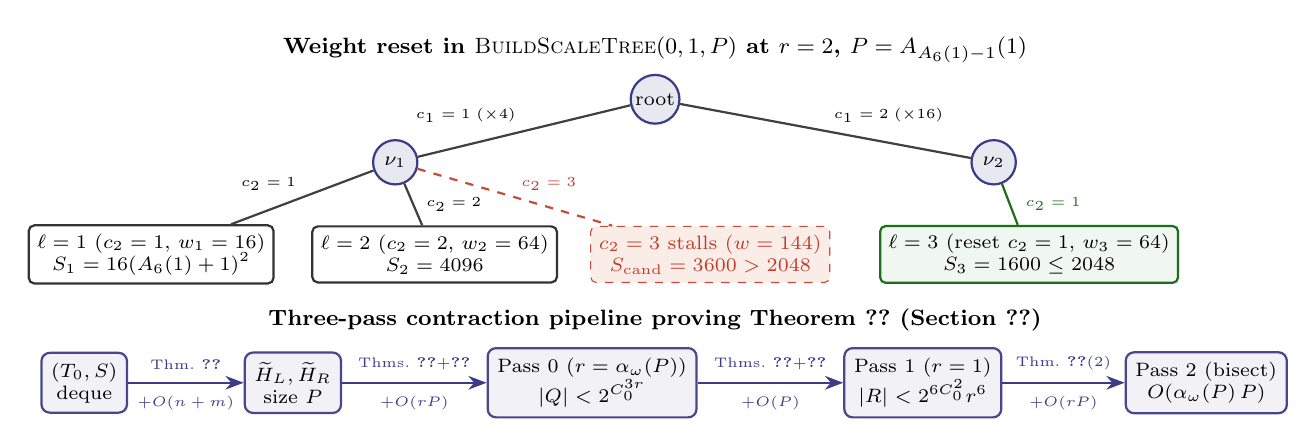
\begin{tikzpicture}[
  >=Stealth,
  tnode/.style={circle, draw=MidnightBlue!85, fill=MidnightBlue!10, thick, minimum size=16pt, inner sep=1pt, font=\scriptsize},
  lnode/.style={rectangle, rounded corners=2pt, draw=black!80, fill=white, thick, inner sep=3pt, font=\scriptsize, align=center},
  stallnode/.style={rectangle, rounded corners=2pt, draw=BrickRed!75, dashed, fill=BrickRed!6, inner sep=3pt, font=\scriptsize, text=BrickRed!85, align=center},
  stagebox/.style={rectangle, rounded corners=3pt, draw=MidnightBlue!80, fill=MidnightBlue!6, thick, inner sep=3.5pt, font=\scriptsize, align=center}
]
  % ---------------- Top: Exact r=2 trace ----------------
  \node[font=\footnotesize\bfseries] at (7.75, 3.25) {Weight reset in $\BuildScaleTree(0, 1, P)$ at $r = 2$, $P = A_{A_6(1)-1}(1)$};

  \node[tnode] (rt) at (7.75, 2.62) {$\mathrm{root}$};
  \node[tnode] (v1) at (4.45, 1.82) {$\nu_1$};
  \node[tnode] (v2) at (12.05, 1.82) {$\nu_2$};

  \draw[thick, draw=black!75] (rt) -- node[above left=-1pt, font=\tiny] {$c_1=1\;(\times 4)$} (v1);
  \draw[thick, draw=black!75] (rt) -- node[above right=-1pt, font=\tiny] {$c_1=2\;(\times 16)$} (v2);

  \node[lnode]     (s1) at (1.35, 0.65) {$\ell=1$ ($c_2=1$, $w_1=16$)\\$S_1 = 16(A_6(1)+1)^2$};
  \node[lnode]     (s2) at (4.95, 0.65) {$\ell=2$ ($c_2=2$, $w_2=64$)\\$S_2 = 4096$};
  \node[stallnode] (st) at (8.45, 0.65) {$c_2=3$ stalls ($w=144$)\\$S_{\mathrm{cand}} = 3600 > 2048$};
  \node[lnode, draw=ForestGreen!80!black, fill=ForestGreen!7] (s3) at (12.50, 0.65) {$\ell=3$ (reset $c_2=1$, $w_3=64$)\\$S_3 = 1600 \le 2048$};

  \draw[thick, draw=black!75] (v1) -- node[above left=-2pt, font=\tiny] {$c_2=1$} (s1);
  \draw[thick, draw=black!75] (v1) -- node[right=1pt, font=\tiny] {$c_2=2$} (s2);
  \draw[thick, dashed, draw=BrickRed!75] (v1) -- node[above right=-2pt, font=\tiny, text=BrickRed!85] {$c_2=3$} (st);
  \draw[thick, draw=ForestGreen!80!black] (v2) -- node[right=2pt, font=\tiny, text=ForestGreen!80!black] {$c_2=1$} (s3);

  % ---------------- Bottom: 3-pass pipeline ----------------
  \node[font=\footnotesize\bfseries] at (7.75, -0.18) {Three-pass contraction pipeline proving Theorem~\ref{thm:main} (Section~\ref{subsec:master-assembly})};

  \node[stagebox] (p0) at (0.50, -0.98) {$(T_0, S)$\\deque};
  \node[stagebox] (p1) at (3.15, -0.98) {$\widetilde{H}_L, \widetilde{H}_R$\\size $P$};
  \node[stagebox] (p2) at (6.95, -0.98) {Pass 0 ($r=\alpha_\omega(P)$)\\$|Q| < 2^{C_0^{3r}}$};
  \node[stagebox] (p3) at (11.15, -0.98) {Pass 1 ($r=1$)\\$|R| < 2^{6C_0^2} r^6$};
  \node[stagebox] (p4) at (14.75, -0.98) {Pass 2 (bisect)\\$O(\alpha_\omega(P)\,P)$};

  \draw[->, thick, MidnightBlue!85] (p0) -- node[above=1pt, font=\tiny] {Thm.~\ref{thm:mod1-reduction}} node[below=1pt, font=\tiny] {$+O(n+m)$} (p1);
  \draw[->, thick, MidnightBlue!85] (p1) -- node[above=1pt, font=\tiny] {Thms.~\ref{thm:mod3-pass}+\ref{thm:mod4-contraction}} node[below=1pt, font=\tiny] {$+O(rP)$} (p2);
  \draw[->, thick, MidnightBlue!85] (p2) -- node[above=1pt, font=\tiny] {Thms.~\ref{thm:mod3-pass}+\ref{thm:mod4-contraction}} node[below=1pt, font=\tiny] {$+O(P)$} (p3);
  \draw[->, thick, MidnightBlue!85] (p3) -- node[above=1pt, font=\tiny] {Thm.~\ref{thm:mod3-pass}(2)} node[below=1pt, font=\tiny] {$+O(rP)$} (p4);
\end{tikzpicture}
\caption{Top: exact trace of $\BuildScaleTree$ at $r = 2$ showing how resetting $c_2 = 1$ under sibling $\nu_2$ drops the candidate weight from $144$ to $64$ so contraction continues past $S_2 = 4096$ to $S_3 = 1600$. Bottom: chaining Sections~\ref{sec:reduction}, \ref{sec:scale-tree}, and~\ref{sec:contraction} across three passes proves Theorem~\ref{thm:main}.}
\label{fig:build-scale-tree}
\end{figure}

\paragraph{Proof overview.}
Given $P \ge 1$ and target height $r \ge 1$, our top-down greedy procedure $\BuildScaleTree$ (Section~\ref{subsec:build-scale-tree}) builds a scale tree $\mathcal{T}$ of height at most $r$ whose leaf parent depth $\delta = r - 1$ greedily appends scales until $S_{\mathrm{cand}} > \frac{1}{2} S_{\mathrm{curr}}$ (contracting block size $S \mapsto \mathrm{poly}(W, \alpha_1(S))$), while each internal depth $\delta = r - q$ ($q \ge 2$) loops over $2\,\alpha_q(S_{\mathrm{in}})$ children so every consecutive pair $(2m - 1, 2m)$ of children decreases $\alpha_q(S_{\mathrm{curr}})$ by at least~$1$ (Lemma~\ref{lem:build-scale-tree} in Section~\ref{subsec:contraction-proof}). Using only Definition~\ref{def:ackermann}, Definition~\ref{def:scale-tree}, and Lemma~\ref{lem:ack-basic}, Section~\ref{subsec:contraction-proof} proves Theorem~\ref{thm:mod4-contraction}, and Section~\ref{subsec:master-assembly} then combines Theorems~\ref{thm:mod1-reduction}, \ref{thm:mod3-pass}, and~\ref{thm:mod4-contraction} to prove Theorem~\ref{thm:main}.

\subsection{The Recursive Scale-Tree Builder \texorpdfstring{$\BuildScaleTree$}{BuildScaleTree}}
\label{subsec:build-scale-tree}

Fix integers $r \ge 1$ and $P \ge 1$. To construct a valid height-$r$ scale tree top-down, we initialize the global scale counter $M := 0$ and coarse block parameters $S_0 := P$ and $\mathcal{P}_0 := \{\{1, \dots, P\}\}$, and call $(\tau_{\mathrm{root}}, S_{\mathrm{out}}) := \BuildScaleTree(0, 1, P)$ at the root. Each recursive call $\BuildScaleTree(\delta, W, S_{\mathrm{in}})$ takes the current tree depth $\delta \in \{0, \dots, r - 1\}$, the accumulated path weight $W \ge 1$ from the root, and the current block-size bound $S_{\mathrm{in}} \ge 1$, and returns a pair $(\tau, S_{\mathrm{out}})$ consisting of either $\tau = \mathrm{EMPTY}$ (when not even one new leaf scale fits under $\frac{1}{2} S_{\mathrm{in}}$) or a non-empty subtree $\tau$, together with the resulting finest block-size bound $S_{\mathrm{out}} \ge 1$. At leaf-parent depth $\delta = r - 1$, it greedily appends leaf scales $c = 1, 2, \dots$ as long as the candidate size $S_{\mathrm{cand}} = 4 c^2 W (\alpha_0(2 S_{\mathrm{curr}}) + 1)^2$ shrinks by at least half; at shallower internal depths $0 \le \delta \le r - 2$ ($q = r - \delta \ge 2$), it sequentially builds up to $2\,\alpha_q(S_{\mathrm{in}})$ child subtrees (each resetting its own child counter from~$1$) until a child stalls:

\begin{center}
\fbox{%
\begin{minipage}{0.94\textwidth}
\vspace{4pt}
\noindent\textbf{Procedure} $\BuildScaleTree(\delta, W, S_{\mathrm{in}})$ \quad ($\delta \in \{0, \dots, r - 1\}$, $W \ge 1$, $S_{\mathrm{in}} \ge 1$)
\begin{itemize}[leftmargin=1.8em, itemsep=3pt, topsep=4pt]
  \item \textbf{Base depth $\delta = r - 1$ ($q := r - \delta = 1$):} Set $S_{\mathrm{curr}} := S_{\mathrm{in}}$. For $c = 1, 2, \dots$:
  \begin{enumerate}[label=\arabic*., leftmargin=1.5em, itemsep=1pt, topsep=2pt]
    \item Set $w_{\mathrm{cand}} := 4 c^2 W$, $i_{\mathrm{cand}} := \alpha_0(2 S_{\mathrm{curr}}) + 1$, and $S_{\mathrm{cand}} := w_{\mathrm{cand}}\, i_{\mathrm{cand}}^2$.
    \item If $S_{\mathrm{cand}} \le \frac{1}{2} S_{\mathrm{curr}}$, increment $M \leftarrow M + 1$, append leaf scale $M$ with parameters $(w_M, i_M, S_M) := (w_{\mathrm{cand}}, i_{\mathrm{cand}}, S_{\mathrm{cand}})$, and update $S_{\mathrm{curr}} \leftarrow S_{\mathrm{cand}}$.
    \item Otherwise ($S_{\mathrm{cand}} > \frac{1}{2} S_{\mathrm{curr}}$), stop the loop: if $c = 1$, return $(\mathrm{EMPTY}, S_{\mathrm{curr}})$; if $c \ge 2$, return $(\nu, S_{\mathrm{curr}})$, where $\nu$ is an internal node whose ordered children are the $c - 1$ leaves appended during this call.
  \end{enumerate}
  \item \textbf{Internal depth $0 \le \delta \le r - 2$ ($q := r - \delta \ge 2$):} Set $m^* := \alpha_q(S_{\mathrm{in}}) \ge 1$, $S_{\mathrm{curr}} := S_{\mathrm{in}}$, and an empty ordered child list $\mathcal{C} := []$. For $c = 1, 2, \dots, 2 m^*$:
  \begin{enumerate}[label=\arabic*., leftmargin=1.5em, itemsep=1pt, topsep=2pt]
    \item Call $(\nu_c, S_{\mathrm{next}}) := \BuildScaleTree(\delta + 1, 4 c^2 W, S_{\mathrm{curr}})$.
    \item If $\nu_c = \mathrm{EMPTY}$, break out of the loop; otherwise append $\nu_c$ to $\mathcal{C}$ and update $S_{\mathrm{curr}} \leftarrow S_{\mathrm{next}}$.
  \end{enumerate}
  Return $(\mathrm{EMPTY}, S_{\mathrm{curr}})$ if $\mathcal{C}$ is empty, and otherwise return $(\nu, S_{\mathrm{curr}})$, where $\nu$ is an internal node with ordered children $\mathcal{C}$.
\end{itemize}
\vspace{2pt}
\end{minipage}%
}
\end{center}

\paragraph{Termination and structural validity.}
Every leaf appended at $\delta = r - 1$ has $w_{\mathrm{cand}} \ge 4$ and $i_{\mathrm{cand}} \ge 2$, so $16 \le S_{\mathrm{cand}} \le \frac{1}{2} S_{\mathrm{curr}}$. In particular, on any call $\BuildScaleTree(\delta, W, S_{\mathrm{in}})$ starting with global counter $\ell_0$, if $L_{\mathrm{loc}} \ge 1$ leaves $\ell_0 + 1, \dots, \ell_0 + L_{\mathrm{loc}}$ are appended during that call, their size bounds satisfy $S_{\mathrm{in}} \ge 2 S_{\ell_0 + 1} \ge \dots \ge 2^{L_{\mathrm{loc}}} S_{\ell_0 + L_{\mathrm{loc}}} \ge 16 \cdot 2^{L_{\mathrm{loc}}}$ (while if $L_{\mathrm{loc}} = 0$ then $S_{\mathrm{out}} = S_{\mathrm{in}} \ge 1$); hence the unbounded loop at $\delta = r - 1$ always terminates, $1 \le S_{\mathrm{out}} \le S_{\mathrm{in}}$, and $\tau = \mathrm{EMPTY}$ if and only if $L_{\mathrm{loc}} = 0$ (in which case $S_{\mathrm{out}} = S_{\mathrm{in}}$).

At the root call $(\tau_{\mathrm{root}}, S_{\mathrm{out}}) := \BuildScaleTree(0, 1, P)$, either $M = 0$ and $\tau_{\mathrm{root}} = \mathrm{EMPTY}$, or $M \ge 1$ and $\mathcal{T} := \tau_{\mathrm{root}} \ne \mathrm{EMPTY}$. Whenever $M \ge 1$, every internal node created at depth $\delta \in \{0, \dots, r - 2\}$ has a non-empty list $\mathcal{C}$ of depth-$(\delta + 1)$ children, and every internal node created at depth $r - 1$ has $c - 1 \ge 1$ leaf children at depth $r$. Because children are visited in left-to-right order and $M$ increments sequentially as leaves are created, the leaves of $\mathcal{T}$ in left-to-right order are precisely $1, \dots, M$, each at depth $\delta(\ell) = r \in \{1, \dots, r\}$, so $\mathcal{T}$ is a scale tree of height $r$ (hence at most $r$). By induction on depth, any call reached from the root along child indices $(c_1, \dots, c_\delta)$ receives $W = \prod_{t=1}^\delta (4 c_t^2)$, so each leaf $\ell$ receives $w_\ell = 4 c_r^2 W = \prod_{t=1}^r (4 c_t^2)$, matching Definition~\ref{def:scale-tree}. Finally, $S_{\mathrm{curr}}$ equals $S_{\ell-1}$ immediately before leaf $\ell$ is appended, so every $\ell \in \{1, \dots, M\}$ satisfies
\[
i_\ell \;=\; \alpha_0(2 S_{\ell-1}) + 1
\qquad\text{and}\qquad
S_\ell \;=\; w_\ell\, i_\ell^2 \;\le\; \frac{1}{2} S_{\ell-1}
\]
(with $S_M = S_{\mathrm{out}} \le 2^{-M} P$, so $M \le \lfloor \log_2 P \rfloor$). Splitting each $X \in \mathcal{P}_{\ell-1}$ ($|X| \in [S_{\ell-1}, 2 S_{\ell-1})$) into $K_X := \lfloor |X| / S_\ell \rfloor \ge 2$ contiguous sub-blocks of size $S_\ell$ (with last sub-block in $[S_\ell, 2 S_\ell)$) therefore yields nested partitions $\mathcal{P}_0 \succ \mathcal{P}_1 \succ \dots \succ \mathcal{P}_M$, and $\mathcal{T}$ validly partitions $\{1, \dots, P\}$ in the sense of Definition~\ref{def:scale-tree}.

\subsection{Degree-6 Contraction Analysis: Proof of Theorem~\ref{thm:mod4-contraction}}
\label{subsec:contraction-proof}

\begin{lemma}[Contraction and Empty-Return Bounds for $\BuildScaleTree$]
\label{lem:build-scale-tree}
Fix integers $r \ge 1$ and $P \ge 1$, and set $C_0 := 6$ and $C_q := 2^{C_0^{2q}} = 2^{36^q}$ for $q \in \{1, \dots, r\}$.
\begin{enumerate}[label=(\arabic*)]
  \item \emph{(Empty-return bound)} Whenever a call $\BuildScaleTree(\delta', W', S')$ ($\delta' \in \{0, \dots, r - 1\}$, $q' := r - \delta' \ge 1$, $W' \ge 1$, $S' \ge 1$) returns $(\mathrm{EMPTY}, S')$, the integer $w := 2 S'$ satisfies
  \[
  w \;<\; 4^{q'+1}\, W'\, \big(\alpha_0(w) + 1\big)^2.
  \]
  \item \emph{(Degree-$6$ contraction)} For every $\delta \in \{0, \dots, r - 1\}$ ($q := r - \delta \in \{1, \dots, r\}$), $W \ge 1$, and $S_{\mathrm{in}} \ge 1$, the output $(\tau, S_{\mathrm{out}})$ of $\BuildScaleTree(\delta, W, S_{\mathrm{in}})$ satisfies
  \[
  2 S_{\mathrm{out}} \;\le\; \Big(\max\big(W,\; \alpha_q(S_{\mathrm{in}}),\; C_q\big)\Big)^{6^q}.
  \]
\end{enumerate}
\end{lemma}

\begin{proof}
We first prove~(1) by induction on $q' = r - \delta' \ge 1$. At $q' = 1$ ($\delta' = r - 1$), the call $\BuildScaleTree(r - 1, W', S')$ returns $\mathrm{EMPTY}$ only if iteration $c = 1$ immediately stops with $S_{\mathrm{curr}} = S'$, meaning $w_{\mathrm{cand}} = 4 W'$, $i_{\mathrm{cand}} = \alpha_0(w) + 1$, and $S_{\mathrm{cand}} = 4 W' (\alpha_0(w) + 1)^2 > \frac{1}{2} S' = \frac{1}{4} w$, i.e., $w < 16 W' (\alpha_0(w) + 1)^2 = 4^{q'+1} W' (\alpha_0(w) + 1)^2$. For $q' \ge 2$, since $m^* = \alpha_{q'}(S') \ge 1$, iteration $c = 1$ always runs and calls $\BuildScaleTree(\delta' + 1, 4 W', S')$; the parent call returns $\mathrm{EMPTY}$ only if this first child returns $\mathrm{EMPTY}$, so the $(q' - 1)$-hypothesis gives $w < 4^{q'} (4 W') (\alpha_0(w) + 1)^2 = 4^{q'+1} W' (\alpha_0(w) + 1)^2$.

Before proving~(2), observe that for every integer $w \ge 2^{216}$, Lemma~\ref{lem:ack-basic}(1) gives $\alpha_0(w) + 1 < \log_2 w + 2$, and setting $z := \log_2 w \ge 216$ and $g(z) := \frac{z}{6}\ln 2 - 2\ln(z + 2)$, we have $(216 + 2)^2 = 47{,}524 < 2^{36} = 2^{216/6}$ (so $g(216) > 0$) and $g'(z) = \frac{\ln 2}{6} - \frac{2}{z + 2} > \frac{0.69}{6} - \frac{2}{218} > 0$ for all $z \ge 216$, whence
\begin{equation}
\label{eq:log-sixth-power}
\big(\alpha_0(w) + 1\big)^2 \;<\; (\log_2 w + 2)^2 \;<\; w^{1/6}
\qquad \text{for all integers } w \ge 2^{216}.
\end{equation}

We now prove~(2) by induction on $q = r - \delta \in \{1, \dots, r\}$.

\paragraph{Base case $q = 1$ ($\delta = r - 1$, $C_1 = 2^{36}$).}
Set $B := \max\big(W, \alpha_1(S_{\mathrm{in}}), 2^{36}\big) \ge 2^{36}$. Let $\ell_0$ be the global leaf count on entry and $L_{\mathrm{loc}} \ge 0$ be the number of leaves $\ell_0 + 1, \dots, \ell_0 + L_{\mathrm{loc}}$ appended during this call; write $\widehat{S}_0 := S_{\mathrm{in}}$ and $\widehat{S}_c := S_{\ell_0 + c}$ for $1 \le c \le L_{\mathrm{loc}}$ (so $S_{\mathrm{out}} = \widehat{S}_{L_{\mathrm{loc}}}$), and set $u_c := \alpha_0(2 \widehat{S}_c)$ ($0 \le c \le L_{\mathrm{loc}}$). By Lemma~\ref{lem:ack-basic}(2), $M^* := \alpha_1(2 S_{\mathrm{in}}) \le \alpha_1(S_{\mathrm{in}}) + 1 \le B + 1$. If $M^* = 1$, then~\eqref{eq:alpha-r} gives $2 S_{\mathrm{out}} \le 2 S_{\mathrm{in}} \le 4 < B^6$. Assume henceforth $M^* \ge 2$, and set $f(u) := \alpha_0(u) + 1$. Whenever $1 \le c \le L_{\mathrm{loc}}$ and $u_{c-1} \ge \max(W, c, 5)$, we have $W \le u_{c-1}$, $c \le u_{c-1}$, and $u_{c-1} + 1 \le 2 u_{c-1}$, so
\[
2 \widehat{S}_c \;=\; 8 W c^2 (u_{c-1} + 1)^2 \;\le\; 8 u_{c-1}^3 (u_{c-1} + 1)^2 \;\le\; 32 u_{c-1}^5 \;<\; 2^{20} u_{c-1}^6,
\]
and Lemma~\ref{lem:ack-basic}(3) ($u_{c-1} \ge 5$) yields $u_c = \alpha_0(2 \widehat{S}_c) \le \alpha_0(2^{20} u_{c-1}^6) \le \alpha_0(u_{c-1}) + 1 = f(u_{c-1})$.

\begin{itemize}[leftmargin=2em]
  \item \emph{Case 1 ($L_{\mathrm{loc}} \ge M^*$):} We claim there exists $c_0 \in \{0, \dots, M^* - 1\}$ with $u_{c_0} \le \max(W, c_0 + 1, 4)$. Indeed, if $u_{c-1} < \max(W, c, 5)$ for some $1 \le c \le M^* - 1$, then $c_0 := c - 1$ satisfies $u_{c_0} \le \max(W, c_0 + 1, 4)$; otherwise $u_{c-1} \ge \max(W, c, 5)$ holds for every $1 \le c \le M^* - 1$, so iterating $u_c \le f(u_{c-1})$ and applying Lemma~\ref{lem:ack-basic}(3) (together with $2 S_{\mathrm{in}} \le F_1(M^*) = F_0^{(M^* - 1)}(4) \implies \alpha_0^{(M^* - 1)}(2 S_{\mathrm{in}}) \le 4$ from Lemma~\ref{lem:ack-basic}(2)) gives
  \[
  u_{M^* - 1} \;\le\; f^{(M^* - 1)}(u_0) \;\le\; \alpha_0^{(M^* - 1)}\big(\alpha_0(2 S_{\mathrm{in}})\big) + 2 \;=\; \alpha_0^{(M^*)}(2 S_{\mathrm{in}}) + 2 \;\le\; \alpha_0(4) + 2 \;=\; 4,
  \]
  so $c_0 := M^* - 1$ satisfies $u_{c_0} \le 4 \le \max(W, c_0 + 1, 4)$. Since $c_0 + 1 \le M^* \le \min(L_{\mathrm{loc}}, B + 1)$ and $u_{c_0} \le \max(W, c_0 + 1, 4) \le B + 1$, monotonicity $\widehat{S}_{L_{\mathrm{loc}}} \le \widehat{S}_{c_0 + 1}$ and $B \ge 2^{36}$ give
  \[
  2 S_{\mathrm{out}} \;\le\; 2 \widehat{S}_{c_0 + 1} \;=\; 8 W (c_0 + 1)^2 (u_{c_0} + 1)^2 \;\le\; 8 B (B + 1)^2 (B + 2)^2 \;<\; B^6.
  \]
  \item \emph{Case 2 ($L_{\mathrm{loc}} \le M^* - 1$):} The loop stops at $c = L_{\mathrm{loc}} + 1 \le M^* \le B + 1$ with $S_{\mathrm{curr}} = S_{\mathrm{out}}$, so $w := 2 S_{\mathrm{out}}$ satisfies
  \[
  w \;<\; 4 S_{\mathrm{cand}} \;=\; 16 W (L_{\mathrm{loc}} + 1)^2 \big(\alpha_0(w) + 1\big)^2 \;\le\; 16 B (B + 1)^2 \big(\alpha_0(w) + 1\big)^2.
  \]
  If $w < 2^{216}$, then $w < (2^{36})^6 \le B^6$. If $w \ge 2^{216}$, then~\eqref{eq:log-sixth-power} gives $(\alpha_0(w) + 1)^2 < w^{1/6}$, so $w^{5/6} < 16 B (B + 1)^2 < B^5$ (as $B \ge 2^{36}$) and hence $w < B^6$.
\end{itemize}

\paragraph{Inductive step $q \ge 2$ ($\delta = r - q$, $C_q = 2^{36^q} \ge 2^{1296}$).}
Set $m^* := \alpha_q(S_{\mathrm{in}}) \ge 1$, $B_q := \max(W, m^*, C_q) \ge 2^{1296}$, and $M_{\mathrm{floor}} := \max\big(16 W (m^*)^2, C_q\big)$. Since $W, m^* \le B_q$ and $B_q \ge 2^{1296}$, we have $M_{\mathrm{floor}} \le 16 B_q^3 < B_q^6$ and thus $M_{\mathrm{floor}}^{6^{q-1}} < B_q^{6^q}$.
\begin{itemize}[leftmargin=2em]
  \item If $m^* = 1$, then~\eqref{eq:alpha-r} gives $S_{\mathrm{in}} \le 4$, so $2 S_{\mathrm{out}} \le 2 S_{\mathrm{in}} \le 8 < B_q^{6^q}$.
  \item If $m^* \ge 2$ and some child $c \in \{1, \dots, 2 m^*\}$ returns $\mathrm{EMPTY}$, let $c$ be the first such child, so $S_{\mathrm{out}}$ equals that child's input $S'$ and its weight is $W_c = 4 c^2 W \le 16 W (m^*)^2 \le 16 B_q^3$ at depth $\delta + 1$ ($q' = q - 1$). By~(1), $w := 2 S_{\mathrm{out}} < 4^q W_c (\alpha_0(w) + 1)^2 \le 16 \cdot 4^q B_q^3 (\alpha_0(w) + 1)^2$. If $w < 2^{216}$, then $w < 2^{1296} \le B_q < B_q^{6^q}$; if $w \ge 2^{216}$, then~\eqref{eq:log-sixth-power} and $16 \cdot 4^q = 2^{4 + 2q} < 2^{2 \cdot 36^q} = C_q^2 \le B_q^2$ give $w^{5/6} < 16 \cdot 4^q B_q^3 < B_q^5$, so $w < B_q^6 < B_q^{6^q}$.
  \item Otherwise $m^* \ge 2$ and all $2 m^*$ children return non-$\mathrm{EMPTY}$ nodes, producing $S_{\mathrm{in}} =: S^{(0)} \ge S^{(1)} \ge \dots \ge S^{(2 m^*)} = S_{\mathrm{out}}$, where each child $c \in \{1, \dots, 2 m^*\}$ runs at depth $\delta + 1$ ($q - 1 \ge 1$) with weight $W_c = 4 c^2 W \le 16 W (m^*)^2 \le M_{\mathrm{floor}}$ (and $C_{q-1} < C_q \le M_{\mathrm{floor}}$). Suppose for contradiction that $2 S_{\mathrm{out}} > M_{\mathrm{floor}}^{6^{q-1}}$; then $2 S^{(c)} > M_{\mathrm{floor}}^{6^{q-1}}$ for every $0 \le c \le 2 m^*$.

  Fix any $m \in \{1, \dots, m^* - 1\}$. Applying the $(q - 1)$-hypothesis to child $2m - 1$ gives
  \[
  M_{\mathrm{floor}}^{6^{q-1}} \;<\; 2 S^{(2m-1)} \;\le\; \Big(\max\big(M_{\mathrm{floor}},\; \alpha_{q-1}(S^{(2m-2)})\big)\Big)^{6^{q-1}},
  \]
  forcing $s_m := \alpha_{q-1}(S^{(2m-2)}) > M_{\mathrm{floor}} \ge 2^{36^q}$ and $2 S^{(2m-1)} \le s_m^{6^{q-1}}$. Write $x := \log_2 s_m > 36^q \ge 1296$. Since $6^{q-1} x > 6 \cdot 1296 > 5$, we have $S^{(2m-1)} + 16 \le \frac{1}{2} s_m^{6^{q-1}} + 16 < s_m^{6^{q-1}} = 2^{6^{q-1} x}$, so Lemma~\ref{lem:ack-basic}(2) (with $\log_2 6 < 3$) gives
  \[
  \alpha_{q-1}(S^{(2m-1)}) \le \alpha_1(S^{(2m-1)}) \le \log_2\log_2(S^{(2m-1)} + 16) + 2 < \log_2(6^{q-1} x) + 2 < \log_2 x + 3q + 1.
  \]
  Because $x > 36^q \ge 1296$ implies $\log_2 x > q \log_2 36 > 5q$ (and $\log_2 x > 10$), we have $3q + 1 < \frac{3}{5}\log_2 x + 1 < \log_2 x$, whence $\log_2 x + 3q + 1 < 2 \log_2 x$. Moreover, $h(z) := z^{1/2} - 2\log_2 z$ satisfies $h(1296) > 36 - 22 > 0$ (as $1296 < 2^{11}$) and $h'(z) = \frac{z^{1/2} - 4/\ln 2}{2z} > 0$ for all $z \ge 1296$, so $2\log_2 x < x^{1/2}$ and thus $\alpha_{q-1}(S^{(2m-1)}) < x^{1/2}$.

  Applying the $(q - 1)$-hypothesis to child $2m$ (where $2 S^{(2m)} > M_{\mathrm{floor}}^{6^{q-1}}$) similarly forces the inequality $\alpha_{q-1}(S^{(2m-1)}) > M_{\mathrm{floor}}$ and
  \[
  2 S^{(2m)} \;\le\; \big(\alpha_{q-1}(S^{(2m-1)})\big)^{6^{q-1}} \;<\; (x^{1/2})^{6^{q-1}} \;=\; 2^{\frac{1}{2} 6^{q-1} \log_2 x}.
  \]
  Since $6^q = (36^q)^{1/2} < x^{1/2}$ and $\log_2 x < \frac{1}{2} x^{1/2}$, we obtain $\frac{1}{2} 6^{q-1} \log_2 x = \frac{1}{12} 6^q \log_2 x < \frac{1}{24} x < x$, whence $S^{(2m)} < 2 S^{(2m)} < 2^x = s_m = \alpha_{q-1}(S^{(2m-2)})$. Because $S^{(2m-2)} > \frac{1}{2} M_{\mathrm{floor}}^{6^{q-1}} > 4$, recursion~\eqref{eq:alpha-r} and monotonicity of $\alpha_q$ give $\alpha_q(S^{(2m-2)}) = 1 + \alpha_q(s_m) \ge 1 + \alpha_q(S^{(2m)})$. Summing over $m = 1, \dots, m^* - 1$ yields
  \[
  1 \;\le\; \alpha_q(S^{(2 m^* - 2)}) \;\le\; \alpha_q(S^{(0)}) - (m^* - 1) \;=\; 1,
  \]
  forcing $S^{(2 m^* - 2)} \le 4$ and contradicting $2 S^{(2 m^* - 2)} > M_{\mathrm{floor}}^{6^{q-1}} > 8$.
\end{itemize}
Hence $2 S_{\mathrm{out}} \le M_{\mathrm{floor}}^{6^{q-1}} < B_q^{6^q}$ in all cases, completing the induction.
\end{proof}

\begin{proof}[Proof of Theorem~\ref{thm:mod4-contraction}]
Take $C_0 := 6$ and execute $(\tau_{\mathrm{root}}, S_{\mathrm{out}}) := \BuildScaleTree(0, 1, P)$ with height parameter $r \ge 1$ ($\delta = 0$, $W = 1$, $q = r$, and $C_r = 2^{C_0^{2r}} = 2^{36^r}$). If $\tau_{\mathrm{root}} = \mathrm{EMPTY}$ ($M = 0$), Lemma~\ref{lem:build-scale-tree}(1) gives $w := 2P < 4^{r+1}(\alpha_0(w) + 1)^2$. Either $w < 2^{216} \le 2^{216^r}$ or $w \ge 2^{216}$, where~\eqref{eq:log-sixth-power} yields $w^{5/6} < 4^{r+1} = 2^{2(r+1)}$ and hence $w < 2^{12(r+1)/5} < 2^{216^r}$; since $216^r = 6^r \cdot 36^r = 6^r C_0^{2r}$, both cases give
\[
2P \;=\; w \;<\; \big(2^{C_0^{2r}}\big)^{6^r} \;\le\; \Big(\max\big(\alpha_r(P),\; 2^{C_0^{2r}}\big)\Big)^{6^r},
\qquad\text{i.e.,}\qquad
P \;<\; \frac{1}{2}\Big(\max\big(\alpha_r(P),\; 2^{C_0^{2r}}\big)\Big)^{6^r}.
\]
Otherwise $M \ge 1$; as verified in Section~\ref{subsec:build-scale-tree}, $\mathcal{T} := \tau_{\mathrm{root}}$ is a scale tree of height at most $r$ validly partitioning $\{1, \dots, P\}$ with $S_M = S_{\mathrm{out}}$, and Lemma~\ref{lem:build-scale-tree}(2) at $(0, 1, P)$ gives $2 S_M \le \big(\max(\alpha_r(P), 2^{C_0^{2r}})\big)^{6^r}$.

In particular, at $r = \alpha_\omega(P)$ we have $\alpha_r(P) \le 2 < 2^{C_0^{2r}}$ and $(2^{C_0^{2r}})^{6^r} = 2^{6^r C_0^{2r}} = 2^{C_0^{3r}}$ (for $C_0 = 6$), so either $P < \frac{1}{2}\cdot 2^{C_0^{3r}} < 2^{C_0^{3r}}$ already or every leaf block $Q \in \mathcal{P}_M$ satisfies $|Q| < 2 S_M \le 2^{C_0^{3r}}$; likewise, at $r = 1$ on any $N_0 \ge 1$, either $N_0 < \frac{1}{2}\max(\alpha_1(N_0), 2^{C_0^2})^6$ already or every leaf block has size $< 2 S_M \le \max(\alpha_1(N_0), 2^{C_0^2})^6$.
\end{proof}

\subsection{Three-Pass Cleanup: Proof of Theorem~\ref{thm:main}}
\label{subsec:master-assembly}

Combining Theorems~\ref{thm:mod1-reduction}, \ref{thm:mod3-pass}, and~\ref{thm:mod4-contraction} immediately yields Theorem~\ref{thm:main}:

\begin{proof}[Proof of Theorem~\ref{thm:main}]
For any folded $\POP$ process $\widetilde{H}$ of size $P \ge 1$, set $r := \alpha_\omega(P) \ge 1$:
\begin{enumerate}[label=(\arabic*)]
  \item \emph{Pass 0 (height $r$):} Applying Theorem~\ref{thm:mod4-contraction} and Theorem~\ref{thm:mod3-pass}(1) at height $r$ (treating $\{\widetilde{H}\}$ itself as a single subprocess at $0$ pass cost when $P < \frac{1}{2}\big(\max(\alpha_r(P), 2^{C_0^{2r}})\big)^{6^r}$) pays at most $C_{\mathrm{pass}}\,r\,P$ and decomposes $\widetilde{H}$ into folded $\POP$ processes $\{\widetilde{H}^{(Q)}\}$ of sizes $1 \le N_0 := |Q| < 2^{C_0^{3r}}$ with $\sum_Q |Q| = P$.
  \item \emph{Pass 1 (height $1$):} Since $C_0 \ge 6$ and $r \ge 1$ give $N_0 + 16 < 2^{C_0^{3r} + 1} \le 2^{2 C_0^{3r}}$, Lemma~\ref{lem:ack-basic} yields $\alpha_1(N_0) \le \log_2\log_2(N_0 + 16) + 2 < 3 r \log_2 C_0 + 3 < 2^{C_0^2}\,r$. Applying Theorem~\ref{thm:mod4-contraction} and Theorem~\ref{thm:mod3-pass}(1) at height~$1$ to each $\widetilde{H}^{(Q)}$ pays at most $C_{\mathrm{pass}}\sum_Q |Q| = C_{\mathrm{pass}}\,P$ and decomposes into folded $\POP$ processes $\{\widetilde{H}^{(R)}\}$ of sizes $1 \le N_1 := |R| < \max\big(\alpha_1(N_0), 2^{C_0^2}\big)^6 \le 2^{6 C_0^2}\,r^6$ with $\sum_{Q, R} |R| = P$.
  \item \emph{Pass 2 (bisection):} For $1 \le N_1 < 2^{6 C_0^2}\,r^6$, Theorem~\ref{thm:mod3-pass}(2) and $\log_2 r < r$ ($r \ge 1$) give $J(\widetilde{H}^{(R)}) \le N_1 \max\big(0, \lceil \log_2 N_1 \rceil - 1\big) \le N_1 \log_2 N_1 < (6 C_0^2 + 6)\,r\,N_1$, so $\sum_{Q, R} J(\widetilde{H}^{(R)}) \le (6 C_0^2 + 6)\,r\,P$.
\end{enumerate}
Since $r \ge 1$, summing gives $J(\widetilde{H}) \le (2 C_{\mathrm{pass}} + 6 C_0^2 + 6)\,\alpha_\omega(P)\,P$; substituting into Theorem~\ref{thm:mod1-reduction} ($J(\emptyset) = 0$ when $d_L = 0$ or $d_R = 0$, and $d_L + d_R \le m$) yields Theorem~\ref{thm:main} with $C := \max(C_{\mathrm{red}},\, 4 C_{\mathrm{pass}} + 12 C_0^2 + 12)$.
\end{proof}




% ============================================================================
\section{Structural Degeneration on the Dyadic Partition}
\label{sec:frontiers}
% ============================================================================

The separating scale $\sep(u, v) \in \{1, \dots, M + 1\}$ and the four-way rotation classification $\mathcal{R}_{\mathrm{int}}(\widetilde{H}) = \mathcal{B}_{\mathrm{leaf}} \sqcup \mathcal{B}_1 \sqcup \mathcal{B}_2 \sqcup \mathcal{B}_3$ of Section~\ref{subsec:bucket-defs} depend only on a nested chain of contiguous-interval partitions $\mathcal{P}_0 \succ \mathcal{P}_1 \succ \dots \succ \mathcal{P}_M$ with $\mathcal{P}_0 = \{\{1, \dots, P\}\}$, and not on the numerical scale law $S_\ell = w_\ell i_\ell^2 \le \frac{1}{2} S_{\ell-1}$ of Definition~\ref{def:scale-tree}. We record how this classification degenerates on the purely combinatorial \emph{dyadic partition}---which repeatedly bisects $\{1, \dots, P\}$ into halves down to singletons---and explain why the scale-tree pass of Section~\ref{sec:scale-tree} does not extend to it.

\begin{proposition}[Degeneration of $\mathcal{B}_{\mathrm{leaf}}$ and $\mathcal{B}_3$ on the Dyadic Partition]
\label{prop:dyadic-collapse}
Given any integer $P \ge 1$, set $M := \lceil \log_2 \max(P, 2) \rceil \ge 1$ and define the \emph{dyadic partition} $\mathcal{P}_0 \succ \mathcal{P}_1 \succ \dots \succ \mathcal{P}_M$ of $\{1, \dots, P\}$ inductively from $\mathcal{P}_0 := \{\{1, \dots, P\}\}$ by splitting each block $X \in \mathcal{P}_{\ell-1}$ ($1 \le \ell \le M$) with $|X| \ge 2$ into $K_X = 2$ contiguous sub-blocks of sizes $\lfloor |X| / 2 \rfloor$ and $\lceil |X| / 2 \rceil$, and keeping singleton blocks $|X| = 1$ intact ($K_X = 1$). Then $\max_{X \in \mathcal{P}_\ell} |X| = \lceil P / 2^\ell \rceil$ for every $0 \le \ell \le M$; in particular, every leaf block $Q \in \mathcal{P}_M$ satisfies $|Q| = 1$. Under the four-way classification $\mathcal{R}_{\mathrm{int}}(\widetilde{H}) = \mathcal{B}_{\mathrm{leaf}} \sqcup \mathcal{B}_1 \sqcup \mathcal{B}_2 \sqcup \mathcal{B}_3$ of Section~\ref{subsec:bucket-defs} with respect to $\mathcal{P}_0 \succ \dots \succ \mathcal{P}_M$, every folded $\POP$ process $\widetilde{H}$ of size $P$ satisfies
\[
\mathcal{B}_{\mathrm{leaf}} \;=\; \emptyset \qquad\text{and}\qquad \mathcal{B}_3 \;=\; \emptyset,
\qquad\text{so}\qquad
\mathcal{R}_{\mathrm{int}}(\widetilde{H}) \;=\; \mathcal{B}_1 \sqcup \mathcal{B}_2
\quad\text{and}\quad
J(\widetilde{H}) \;=\; |\mathcal{B}_1| + |\mathcal{B}_2|.
\]
\end{proposition}

\begin{proof}
We prove $\max_{X \in \mathcal{P}_\ell} |X| = \lceil P / 2^\ell \rceil$ by induction on $\ell \in \{0, \dots, M\}$. At $\ell = 0$, $\mathcal{P}_0 = \{\{1, \dots, P\}\}$ has size $P = \lceil P / 2^0 \rceil$. For $1 \le \ell \le M$, each $X \in \mathcal{P}_{\ell-1}$ produces sub-blocks in $\mathcal{P}_\ell$ of maximum size $\lceil |X| / 2 \rceil$ (both for $|X| \ge 2$ and for $|X| = 1$). Since $t \mapsto \lceil t / 2 \rceil$ is non-decreasing and $\big\lceil \lceil a / 2^{\ell-1} \rceil / 2 \big\rceil = \lceil a / 2^\ell \rceil$ for every integer $a \ge 1$, the induction hypothesis gives $\max_{Y \in \mathcal{P}_\ell} |Y| = \big\lceil (\max_{X \in \mathcal{P}_{\ell-1}} |X|) / 2 \big\rceil = \lceil P / 2^\ell \rceil$. At $\ell = M = \lceil \log_2 \max(P, 2) \rceil$, we have $0 < P / 2^M \le 1$, so $\max_{Q \in \mathcal{P}_M} |Q| = \lceil P / 2^M \rceil = 1$ and hence $|Q| = 1$ for every $Q \in \mathcal{P}_M$.

Now consider any internal $\POP$ rotation $e = (x, y, z) \in \mathcal{R}_{\mathrm{int}}(\widetilde{H})$ executed during $\POP(s)$, so $1 \le s < x < y < z \le P$. Because $|Q| = 1$ for every $Q \in \mathcal{P}_M$, distinct keys $x < y$ cannot share a leaf block in $\mathcal{P}_M$, giving $\sep(x, y) \le M$ and $\mathcal{B}_{\mathrm{leaf}} = \emptyset$. Suppose $e \in \mathcal{B}_3$, so $\ell := \sep(s, x) = \sep(x, y) \in \{1, \dots, M\}$. Then $\sep(s, y) = \min\big(\sep(s, x), \sep(x, y)\big) = \ell > \ell - 1$, so $s < x < y$ lie in a common parent block $X \in \mathcal{P}_{\ell-1}$, whereas $\sep(s, x) = \sep(x, y) = \ell$ places $s, x, y$ into three distinct contiguous scale-$\ell$ sub-blocks $S_p < S_b < S_q$ of $X$, contradicting $K_X \le 2$. Thus $\mathcal{B}_3 = \emptyset$, leaving $\mathcal{R}_{\mathrm{int}}(\widetilde{H}) = \mathcal{B}_1 \sqcup \mathcal{B}_2$ and $J(\widetilde{H}) = |\mathcal{B}_1| + |\mathcal{B}_2|$.
\end{proof}

\begin{remark}[Why Section~\ref{sec:scale-tree} Does Not Bound the Dyadic Partition]
\label{rem:dyadic-obstacle}
Proposition~\ref{prop:dyadic-collapse} is purely a structural observation that $\mathcal{B}_{\mathrm{leaf}}$ and $\mathcal{B}_3$ vanish on the dyadic chain---so asking for $|\mathcal{B}_1| + |\mathcal{B}_2| = O(P)$ on the dyadic partition is simply a restatement of $J(\widetilde{H}) = O(P)$ (which would imply $\Rot(T_0, S) = O(m + n)$ via Theorem~\ref{thm:mod1-reduction}), rather than a non-trivial reduction. Two distinct obstacles prevent the scale-tree pass of Theorem~\ref{thm:mod3-pass}(1) from bounding $|\mathcal{B}_1| + |\mathcal{B}_2|$ on the dyadic chain:
\begin{enumerate}[label=(\arabic*)]
  \item \emph{Loss of the internal-node sink bound $\Sigma_{\mathcal{T}} = O(P)$:} In Section~\ref{subsec:tree-weights}, bounding the freeze-sink sum $\Sigma_{\mathcal{T}} = \sum_{\nu \in \mathcal{T}_{\mathrm{int}}} k_\nu |\mathcal{P}_{M_{\mathrm{end}}(\nu)}| = O(P)$ relies directly on the numerical scale law $S_\ell = w_\ell i_\ell^2 \ge 16 k_\nu^2 w(\nu)$ at $\ell = M_{\mathrm{end}}(\nu)$. On the dyadic partition at $P = 2^M$ ($M = \log_2 P$ and $|\mathcal{P}_\ell| = 2^\ell$), a flat height-$1$ tree has $k_{\mathrm{root}} = M$ and $M_{\mathrm{end}}(\mathrm{root}) = M$, giving $\Sigma_{\mathcal{T}} = M P = P \log_2 P$; even on a balanced binary scale tree of height $r = \lceil \log_2 M \rceil$, every internal node $\nu$ along the rightmost root-to-$M$ path has $k_\nu = 2$ and $|\mathcal{P}_{M_{\mathrm{end}}(\nu)}| = |\mathcal{P}_M| = P$, giving $\Sigma_{\mathcal{T}} = \Theta(P \log M) = \Theta(P \log\log P)$.
  \item \emph{Tree-height amplification in $\LCA_{\mathcal{T}}$ chain routing:} At $P = 2^M$ ($M \ge 2$), while a lopsided left-leaning caterpillar tree (placing leaf $M - d$ at depth $d + 1$ for $0 \le d \le M - 3$ and leaves $1, 2$ as siblings at depth $M - 1$) keeps $\Sigma_{\mathcal{T}} < 4P$, it forces tree height $r = M - 1 = \log_2 P - 1$, and the ancestor/descendant chain arguments of Sections~\ref{subsec:b1} and~\ref{subsec:b2-master} multiply the sink bounds $|\mathcal{S}_1|$ and $|\mathcal{S}_2|$ by the height $r$.
\end{enumerate}
\end{remark}


\section*{AI Disclosure}
A Gemini~4 Carbon model with harnesses on top discovered the proof with slight human guidance (Goran \v{Z}u\v{z}i\'{c}, David P.~Woodruff, and Vahab Mirrokni). Goran \v{Z}u\v{z}i\'{c} and Sorrachai Yingchareonthawornchai cleaned up the paper, and Goran \v{Z}u\v{z}i\'{c}, David P.~Woodruff, and Vahab Mirrokni prepared the Lean~4 verification.


% ============================================================================
\appendix
\section{Elementary Properties of the Star-Iterated Inverse-Ackermann Hierarchy}
\label{app:ackermann}
% ============================================================================

This appendix provides complete, self-contained proofs of the elementary Ackermann estimates used in Sections~\ref{sec:reduction}--\ref{sec:contraction} (following Sundar's indexing~\cite[Section~1.2]{Sundar1992}), Proposition~\ref{prop:omega-properties}, and the L\"{o}b--Wainer fast-growing hierarchy comparison stated in Remark~\ref{rem:lob-wainer}.

\begin{lemma}[Elementary Ackermann and Iterated-Inverse Estimates]
\label{lem:ack-basic}
The functions $A_i$, $\alpha_0$, and $\alpha_r$ of Definition~\ref{def:ackermann} satisfy:
\begin{enumerate}[label=(\arabic*)]
  \item For all $i \ge 0$ and $j \ge 1$, $A_i(j) > j$ and $A_i(j)$ is strictly increasing in $j$; for all $i \ge 1$ and $j \ge 1$, $A_i(j) \ge A_{i-1}(j)$ and $A_i(j) \ge 2^j$; and $A_k(1) \ge 2^k$ for all $k \ge 1$. Consequently, $\alpha_0$ is well-defined and non-decreasing with $\alpha_0(1) = 1$, $\alpha_0(n) \le \lceil \log_2 n \rceil < \log_2 n + 1$ for all $n \ge 2$, and $\alpha_0(n) < n$ for all $n \ge 3$.
  \item Setting $F_0(k) := A_k(1)$ ($k \ge 1$) and $F_r(1) := 4$, $F_r(k) := F_{r-1}\big(F_r(k - 1)\big)$ ($r \ge 1, k \ge 2$), we have $F_r(k) \ge 2^k$ for all $r \ge 0$ and $k \ge 1$, with $F_r(k)$ strictly increasing in $k$ and non-decreasing in $r \ge 1$. For every $r \ge 1$, $\alpha_r$ is well-defined and non-decreasing with $\alpha_r(n) < n$ for all $n > 4$ (so Definition~\ref{def:ackermann}'s star-operator condition holds at every $r \ge 1$), and for all integers $r, k, n \ge 1$,
  \[
  \alpha_r(n) \le k \;\Longleftrightarrow\; n \le F_r(k),
  \quad
  \alpha_1(2n) \le \alpha_1(n) + 1,
  \quad
  \alpha_r(n) \le \alpha_1(n) \le \log_2\log_2(n + 16) + 2,
  \]
  and $\alpha_\omega(n) = \min\{r \ge 1 : F_r(2) \ge n\}$.
  \item $\alpha_0(n + 2) \le \alpha_0(n) + 1$ for all $n \ge 1$---consequently, $f(u) := \alpha_0(u) + 1$ satisfies $f^{(m)}(u) \le \alpha_0^{(m)}(u) + 2$ for all $m, u \ge 1$---and $\alpha_0(2^{20} u^6) \le \alpha_0(u) + 1$ for all $u \ge 5$.
\end{enumerate}
\end{lemma}

\begin{proof}
(1) At $i = 0$ and $i = 1$, $A_0(j) = 2j > j$ and $A_1(j) = 2^j \ge 2j = A_0(j) > j$ are strictly increasing in $j \ge 1$. Inducting on $i \ge 2$, assume $A_{i-1}$ is strictly increasing with $A_{i-1}(m) > m$. Then $A_i(1) = A_{i-1}(2) > 2 > 1$, and for $j \ge 2$, $A_i(j) = A_{i-1}(A_i(j - 1)) > A_i(j - 1)$, proving strict monotonicity in $j$ and $A_i(j) > j$. Moreover, $A_i(1) = A_{i-1}(2) > A_{i-1}(1)$, and for $j \ge 2$ inductively $A_i(j - 1) \ge A_{i-1}(j - 1) \ge j$, so strict monotonicity of $A_{i-1}$ gives $A_i(j) = A_{i-1}(A_i(j - 1)) \ge A_{i-1}(j)$, chaining to $A_i(j) \ge A_1(j) = 2^j$. For $A_k(1) \ge 2^k$, note $A_1(1) = 2$, $A_2(1) = A_1(2) = 4$, and for $k \ge 3$ inductively $A_k(1) = A_{k-1}(2) = A_{k-2}(A_{k-1}(1)) \ge 2^{A_{k-1}(1)} \ge 2 A_{k-1}(1) \ge 2^k$. Since $A_{k+1}(1) = A_k(2) > A_k(1)$ is strictly increasing and unbounded with $A_1(1) = 2$, $\alpha_0$ is well-defined and non-decreasing with $\alpha_0(1) = 1$; for $n \ge 2$, $A_{\lceil \log_2 n \rceil}(1) \ge 2^{\lceil \log_2 n \rceil} \ge n$ gives $\alpha_0(n) \le \lceil \log_2 n \rceil < \log_2 n + 1$, and for $n \ge 3$, $\lceil \log_2 n \rceil < n$ gives $\alpha_0(n) < n$.

(2) At $r = 0$, $F_0(k) = A_k(1) \ge 2^k$ is strictly increasing in $k$ by~(1). Inducting on $r \ge 1$, we have $F_r(1) = 4 > 2^1$, and for $k \ge 2$ inductively $F_r(k - 1) \ge 2^{k-1} \ge k$, so $F_r(k) = F_{r-1}(F_r(k - 1)) \ge 2^{F_r(k - 1)} > F_r(k - 1)$ with $2^{F_r(k - 1)} \ge 2^k$. For $r \ge 2$, $F_r(1) = 4 = F_{r-1}(1)$, and for $k \ge 2$ inductively $F_r(k - 1) \ge F_{r-1}(k - 1) \ge 2^{k-1} \ge k$ yields $F_r(k) = F_{r-1}(F_r(k - 1)) \ge F_{r-1}(k)$.

Next we prove by induction on $r \ge 1$ that $\alpha_r$ is well-defined and non-decreasing, satisfies $\alpha_r(n) \le k \iff n \le F_r(k)$ for all $k, n \ge 1$, and satisfies $\alpha_r(n) < n$ for all $n > 4$. At the input to $r$, $\alpha_{r-1}$ is well-defined and non-decreasing with $\alpha_{r-1}(n) < n$ for all $n > 4$ and $\alpha_{r-1}(n) \le m \iff n \le F_{r-1}(m)$ (by~(1) when $r = 1$, and by the $(r - 1)$-hypothesis when $r \ge 2$). Hence~\eqref{eq:alpha-r} terminates on every $n \ge 1$ and (by strong induction on $n$) defines a non-decreasing function $\alpha_r$. Inducting on $k \ge 1$: at $k = 1$, $\alpha_r(n) \le 1 \iff n \le 4 = F_r(1)$ by~\eqref{eq:alpha-r}; for $k \ge 2$, both sides hold when $n \le 4$, and when $n > 4$ we have $\alpha_r(n) \le k \iff \alpha_r(\alpha_{r-1}(n)) \le k - 1 \iff \alpha_{r-1}(n) \le F_r(k - 1) \iff n \le F_{r-1}(F_r(k - 1)) = F_r(k)$. For any $n \ge 5$, $F_r(n - 1) \ge 2^{n-1} > n$ implies $\alpha_r(n) \le n - 1 < n$, closing the induction on $r$.

Setting $k = 2$ gives $\alpha_r(n) \le 2 \iff n \le F_r(2)$, and since $F_{r+1}(2) = F_r(4) > F_r(2)$ grows strictly with $r$, $\alpha_\omega(n) = \min\{r \ge 1 : F_r(2) \ge n\}$ is well-defined for all $n \ge 1$. For $k = \alpha_1(n) \ge 1$, $F_1(k) \ge 4$ gives $F_1(k + 1) = A_{F_1(k)}(1) \ge 2^{F_1(k)} > 2 F_1(k) \ge 2n$, so $\alpha_1(2n) \le k + 1$. Since $F_r(k) \ge F_1(k)$, we have $\alpha_r(n) \le \alpha_1(n)$. Observe by induction on $j \ge 1$ that $A_2(j) \ge 2^{2^j}$ ($A_2(1) = 4 = 2^{2^1}$, and $A_2(j + 1) = 2^{A_2(j)} \ge 2^{2^{2^j}} \ge 2^{2^{j+1}}$ since $2^j \ge j + 1$), and for $m \ge 4$ that $A_m(1) = A_{m-2}(A_{m-1}(1)) \ge A_2(2^{m-1}) \ge A_2(m) \ge 2^{2^m}$. If $n \le F_1(2) = A_4(1)$, then $\alpha_1(n) \le 2 < \log_2\log_2(n + 16) + 2$; if $n > F_1(2)$, then $k := \alpha_1(n) \ge 3$ and $m := F_1(k - 2) \ge \max(4, k - 2)$ give $n > F_1(k - 1) = A_m(1) \ge 2^{2^m} \ge 2^{2^{k-2}}$, so $\log_2\log_2(n + 16) > k - 2$, i.e., $\alpha_1(n) < \log_2\log_2(n + 16) + 2$.

(3) Let $k := \alpha_0(n) \ge 1$, so $n \le A_k(1)$ and $A_k(1) \ge 2$. Then $A_{k+1}(1) = A_k(2) \ge 2 A_k(1) \ge A_k(1) + 2 \ge n + 2$ (at $k = 1$, $A_1(2) = 4 = 2 A_1(1)$, and for $k \ge 2$, $A_k(2) = A_{k-1}(A_k(1)) \ge A_0(A_k(1)) = 2 A_k(1)$), so $\alpha_0(n + 2) \le k + 1$. By induction on $m \ge 1$, $f^{(1)}(u) = \alpha_0(u) + 1 < \alpha_0(u) + 2$ and $f^{(m+1)}(u) = \alpha_0(f^{(m)}(u)) + 1 \le \alpha_0(\alpha_0^{(m)}(u) + 2) + 1 \le \alpha_0^{(m+1)}(u) + 2$. Finally, for $u \ge 5$, since $A_2(1) = 4 < u$, we have $k := \alpha_0(u) \ge 3$ and $u \le A_k(1)$. If $k = 3$, then $u \le A_3(1) = A_2(2) = 16$, so $2^{20} u^6 \le 2^{44} < 2^{65536} = A_2(4) < A_2(16) = A_3(2) = A_4(1)$ (as $A_2(3) = 2^{16} = 65{,}536$), giving $\alpha_0(2^{20} u^6) \le 4 = k + 1$. If $k \ge 4$, then $u > A_3(1) = 16$, so $u \ge 17$ and $20 + 6\log_2 u < 20 + 6u < 2^u$, whence $2^{20} u^6 < 2^{2^u} \le A_2(u) \le A_2(A_k(1)) \le A_{k-1}(A_k(1)) = A_k(2) = A_{k+1}(1)$ and $\alpha_0(2^{20} u^6) \le k + 1$.
\end{proof}

\begin{proof}[Proof of Proposition~\ref{prop:omega-properties}]
Since $A_3(1) = A_2(2) = 16$ and $A_2(3) = 2^{16} = 65{,}536$, we have $F_1(2) = F_0(4) = A_4(1) = A_3(2) = A_2(16) > A_2(4) = 2^{65536}$. By Lemma~\ref{lem:ack-basic}(2), $\alpha_\omega(n) = \min\{r \ge 1 : F_r(2) \ge n\}$ is non-decreasing with $\alpha_\omega(n) = 1$ for all $1 \le n \le A_4(1)$, and since each $F_r(2)$ is finite while $F_{r+1}(2) = F_r(4) > F_r(2)$, $\lim_{n \to \infty} \alpha_\omega(n) = \infty$.

Observe next that $F_t(2) > 2^{t+2}$ for all $t \ge 1$: at $t = 1$, $F_1(2) = A_4(1) > 2^3$, and inductively for $t \ge 2$, Lemma~\ref{lem:ack-basic}(2) gives $F_t(2) = F_{t-1}(4) = F_{t-2}(F_{t-1}(3)) \ge 2^{F_{t-1}(3)} > 2^{F_{t-1}(2)} > 2^{2^{t+1}} \ge 2^{t+2}$. Fix any $r \ge 1$; for every $n > F_{r+2}(2)$, setting $s := \alpha_\omega(n) \ge r + 3$ (so $s - 3 \ge r$ and $s - 2 \ge 2$) and using minimality of $s$ together with Lemma~\ref{lem:ack-basic}(2) yields
\[
n \;>\; F_{s-1}(2) \;=\; F_{s-2}(4) \;>\; F_{s-2}(3) \;=\; F_{s-3}\big(F_{s-2}(2)\big) \;\ge\; F_r\big(F_{s-2}(2)\big) \;\ge\; F_r(2^s).
\]
Hence $\alpha_r(n) > 2^s = 2^{\alpha_\omega(n)}$, i.e., $\alpha_\omega(n) < \log_2 \alpha_r(n)$ for all $n > F_{r+2}(2)$; since $\alpha_r(n) \to \infty$ as $n \to \infty$, $\alpha_\omega(n) = o\big(\alpha_r(n)\big)$.

For the diagonal Ackermann variant, set $\widetilde{F}_0(k) := A_k(k)$ ($k \ge 1$) and $\widetilde{F}_r(1) := 4$, $\widetilde{F}_r(k) := \widetilde{F}_{r-1}\big(\widetilde{F}_r(k - 1)\big)$ ($r \ge 1, k \ge 2$). By Lemma~\ref{lem:ack-basic}(1), $\widetilde{F}_0(k) = A_k(k) \ge A_k(1) = F_0(k) \ge 2^k$ is strictly increasing in $k$ ($A_{k+1}(k + 1) > A_{k+1}(k) \ge A_k(k)$), so $\widetilde{\alpha}_0(n) = \min\{k \ge 1 : \widetilde{F}_0(k) \ge n\} \le \alpha_0(n)$ satisfies $\widetilde{\alpha}_0(n) < n$ for all $n > 4$. Repeating the induction of Lemma~\ref{lem:ack-basic}(2) verbatim shows that $\widetilde{F}_r(k) \ge F_r(k) \ge 2^k$ is strictly increasing in $k$ and non-decreasing in $r \ge 1$, and that each $\widetilde{\alpha}_r$ ($r \ge 1$) defined by~\eqref{eq:alpha-r} is well-defined and non-decreasing with $\widetilde{\alpha}_r(n) < n$ for $n > 4$ and $\widetilde{\alpha}_r(n) \le k \iff n \le \widetilde{F}_r(k)$. In particular, $\widetilde{\alpha}_r(n) \le r \iff n \le \widetilde{F}_r(r)$, so $\widetilde{\alpha}_{\omega,\mathrm{diag}}(n) = \min\{r \ge 1 : \widetilde{F}_r(r) \ge n\}$.

For $k \ge 1$, since $k < 2^{k+1} \le A_{k+1}(1)$, strict monotonicity of $A_k$ gives $F_0(k) = A_k(1) \le A_k(k) = \widetilde{F}_0(k) < A_k(A_{k+1}(1)) = A_{k+1}(2) = A_{k+2}(1) = F_0(k + 2)$. We claim $F_r(k) \le \widetilde{F}_r(k) \le F_r(2k - 1)$ for all $r, k \ge 1$ by induction on $r$ and $k$: at $k = 1$, $F_r(1) = 4 = \widetilde{F}_r(1)$; and if $\widetilde{F}_r(k) \le M := F_r(2k - 1)$ ($M \ge 4$), then $F_r(2k) = F_{r-1}(M) \ge 2^M > \max(M + 2, 2M - 1) \ge \max(\widetilde{F}_r(k) + 2, 2\widetilde{F}_r(k) - 1)$, giving $\widetilde{F}_1(k + 1) = \widetilde{F}_0(\widetilde{F}_1(k)) \le F_0(\widetilde{F}_1(k) + 2) \le F_0(F_1(2k)) = F_1(2k + 1)$ at $r = 1$ and $\widetilde{F}_r(k + 1) = \widetilde{F}_{r-1}(\widetilde{F}_r(k)) \le F_{r-1}(2\widetilde{F}_r(k) - 1) \le F_{r-1}(F_r(2k)) = F_r(2k + 1)$ for $r \ge 2$. Finally, for every $r \ge 1$, $F_r(2) \le F_{r+1}(2) \le \widetilde{F}_{r+1}(2) \le \widetilde{F}_{r+1}(r + 1)$ implies $\widetilde{\alpha}_{\omega,\mathrm{diag}}(n) \le \alpha_\omega(n) + 1$, while $F_{r+1}(3) > F_{r+1}(2) > 2^{r+3} > 2r - 1$ implies $\widetilde{F}_r(r) \le F_r(2r - 1) < F_r(F_{r+1}(3)) = F_{r+1}(4) = F_{r+2}(2)$, yielding $\alpha_\omega(n) \le \widetilde{\alpha}_{\omega,\mathrm{diag}}(n) + 2$.
\end{proof}

\begin{proposition}[Position of $\alpha_0$, $\alpha_r$, and $\alpha_\omega$ in the L\"{o}b--Wainer Fast-Growing Hierarchy]
\label{prop:lob-wainer}
Let $\{f_\beta : \mathbb{Z}_{\ge 1} \to \mathbb{Z}_{\ge 1}\}_{\beta \le \omega \cdot 2}$ be the standard fast-growing (L\"{o}b--Wainer) hierarchy (originating in~\cite{LobWainer1970I,LobWainer1970II}), defined by $f_0(n) := n + 1$, $f_{\beta+1}(n) := f_\beta^{(n)}(n)$, $f_\omega(n) := f_n(n)$, and $f_{\omega \cdot 2}(r) := f_{\omega + r}(r)$, with inverses $f_\beta^{-1}(n) := \min\{k \ge 1 : f_\beta(k) \ge n\}$. Then for every integer $n \ge 1$ and every integer $r \ge 1$,
\[
f_\omega^{-1}(n) \;\le\; \alpha_0(n) \;\le\; f_\omega^{-1}(n) + 2,
\qquad
\frac{1}{3}\,\alpha_r(n) \;\le\; f_{\omega + r}^{-1}(n) \;\le\; \max\big(\alpha_r(n),\, 2\big),
\]
and
\[
f_{\omega \cdot 2}^{-1}(n) - 1 \;\le\; \alpha_\omega(n) \;\le\; f_{\omega \cdot 2}^{-1}(n) + 2.
\]
\end{proposition}

\begin{proof}
First, we verify by transfinite induction on $\beta \le \omega \cdot 2$ that $f_\beta(1) = 2$, $f_\beta(n) > n$ for all $n \ge 1$, $f_\beta$ is strictly increasing, and $f_{\beta+1}(n) \ge f_\beta(n)$ for $\beta < \omega \cdot 2$. At $\beta = 0$, $f_0(1) = 2$ and $f_0(n) = n + 1 > n$ is strictly increasing. If these properties hold at $\beta$, then $f_{\beta+1}(1) = f_\beta^{(1)}(1) = f_\beta(1) = 2$, and since $x \mapsto f_\beta^{(t)}(x)$ is strictly increasing with $f_\beta^{(t+1)}(x) > f_\beta^{(t)}(x) \ge f_\beta(x) > x$, we have $f_{\beta+1}(n) = f_\beta^{(n)}(n) \ge f_\beta(n) > n$ and $f_{\beta+1}(n + 1) = f_\beta^{(n+1)}(n + 1) > f_\beta^{(n)}(n + 1) > f_\beta^{(n)}(n) = f_{\beta+1}(n)$. At the limit levels, $f_\omega(1) = f_1(1) = 2$, $f_\omega(n) = f_n(n) > n$, and $f_\omega(n + 1) = f_{n+1}(n + 1) \ge f_n(n + 1) > f_n(n) = f_\omega(n)$; identically, $f_{\omega \cdot 2}(1) = f_{\omega + 1}(1) = 2$, $f_{\omega \cdot 2}(r) = f_{\omega + r}(r) > r$, and $f_{\omega \cdot 2}(r + 1) = f_{\omega + r + 1}(r + 1) \ge f_{\omega + r}(r + 1) > f_{\omega + r}(r) = f_{\omega \cdot 2}(r)$. Thus $f_\beta^{-1}(n)$ is well-defined for all $\beta \le \omega \cdot 2$ and $n \ge 1$, with $f_\beta^{-1}(n) \le k \iff n \le f_\beta(k)$.

\emph{Step 1 (Finite levels).} Note $f_1(n) = 2n = A_0(n)$ and $f_2(n) = n 2^n$. We prove $f_{m+1}(n) \ge A_m(n)$ for all $m \ge 1$ and $n \ge 2$ by induction on $m$: at $m = 1$, $f_2(n) = n 2^n > 2^n = A_1(n)$; for $m \ge 2$, setting $y_t := f_m^{(t)}(n)$, the $(m - 1)$-hypothesis gives $y_1 = f_m(n) \ge A_{m-1}(n) \ge A_{m-1}(2) = A_m(1) \ge 4 \ge 2$, and inductively $y_t \ge A_m(t) \ge 2$ implies $y_{t+1} = f_m(y_t) \ge A_{m-1}(y_t) \ge A_{m-1}(A_m(t)) = A_m(t + 1)$, so $f_{m+1}(n) = y_n \ge A_m(n)$. Next we prove $f_m(u) \le A_m(3u)$ for all $m \ge 2$ and $u \ge 1$ by induction on $m$: at $m = 2$, using $A_2(j) \ge 2^{2^j}$ from the proof of Lemma~\ref{lem:ack-basic}(2), $f_2(u) = u 2^u < 2^{2u} < 2^{2^{3u}} \le A_2(3u)$. For $m \to m + 1$ ($m \ge 2$), $f_{m+1}(1) = 2 < A_{m+1}(3)$; for $u \ge 2$, setting $x_t := f_m^{(t)}(u)$ ($0 \le t \le u$), we have $x_0 = u < A_{m+1}(u)$, and if $x_t \le M := A_{m+1}(u + 2t)$, then $m + 1 \ge 3$ and $u + 2t \ge 2$ give $M \ge A_3(2) = A_4(1) > 16$, so $3 x_t \le 3 M < 2^M \le A_m(M) = A_{m+1}(u + 2t + 1)$ and $x_{t+1} = f_m(x_t) \le A_m(3 x_t) \le A_m(A_{m+1}(u + 2t + 1)) = A_{m+1}(u + 2t + 2)$, giving $f_{m+1}(u) = x_u \le A_{m+1}(3u)$.

\emph{Step 2 (Level $\omega$).} At $k = 1$, $F_0(1) = A_1(1) = 2 = f_1(1) = f_\omega(1) < 16 = A_3(1) = F_0(3)$. For $k \ge 2$, Step~1 gives $f_\omega(k) = f_k(k) \ge A_{k-1}(k) \ge A_{k-1}(2) = A_k(1) = F_0(k)$, and since $3k < 2^{k+1} \le A_{k+1}(1)$, $f_\omega(k) = f_k(k) \le A_k(3k) < A_k(A_{k+1}(1)) = A_{k+1}(2) = A_{k+2}(1) = F_0(k + 2)$. Thus $F_0(k) \le f_\omega(k) \le F_0(k + 2)$ for all $k \ge 1$, which inverts immediately to $f_\omega^{-1}(n) \le \alpha_0(n) \le f_\omega^{-1}(n) + 2$.

\emph{Step 3 (Levels $\omega + r$, $r \ge 1$).} Writing $\omega + 0 := \omega$, we prove $F_r(k) \le f_{\omega + r}(k)$ for all $r \ge 1$ and $k \ge 2$ by induction on $r$. Fix $k \ge 2$ and set $y_t := f_{\omega + r - 1}^{(t)}(k)$ ($1 \le t \le k$). At $t = 1$: if $r = 1$, $y_1 = f_\omega(k) \ge f_\omega(2) = f_2(2) = 8 \ge 4 = F_1(1)$; if $r \ge 2$, the $(r - 1)$-hypothesis gives $y_1 = f_{\omega + r - 1}(k) \ge F_{r-1}(k) \ge F_{r-1}(2) \ge F_1(2) = A_4(1) > 4 = F_r(1)$. Inductively for $1 \le t < k$, $y_t \ge F_r(t) \ge 4 \ge 2$ gives $y_{t+1} = f_\omega(y_t) \ge F_0(y_t) \ge F_0(F_1(t)) = F_1(t + 1)$ when $r = 1$ (by Step~2) and $y_{t+1} = f_{\omega + r - 1}(y_t) \ge F_{r-1}(y_t) \ge F_{r-1}(F_r(t)) = F_r(t + 1)$ when $r \ge 2$, so $f_{\omega + r}(k) = y_k \ge F_r(k)$.

Conversely, we prove $f_{\omega + r}(u) \le F_r(3u)$ for all $r \ge 1$ and $u \ge 1$ by induction on $r$. At $u = 1$, $f_{\omega + r}(1) = 2 < 4 = F_r(1) < F_r(3)$. For $u \ge 2$, set $x_t := f_{\omega + r - 1}^{(t)}(u)$ ($0 \le t \le u$); then $x_0 = u < 2^u \le F_r(u)$, and if $x_t \le M := F_r(u + 2t)$, then $u + 2t \ge 2$ implies $M \ge F_r(2) \ge A_4(1) > 16$, so $\max(x_t + 2, 3 x_t) \le 3M < 2^M \le F_{r-1}(M) = F_r(u + 2t + 1)$ (Lemma~\ref{lem:ack-basic}(2)). Applying Step~2 at $r = 1$ ($x_{t+1} = f_\omega(x_t) \le F_0(x_t + 2) \le F_0(F_1(u + 2t + 1)) = F_1(u + 2t + 2)$) and the $(r - 1)$-hypothesis for $r \ge 2$ ($x_{t+1} = f_{\omega + r - 1}(x_t) \le F_{r-1}(3 x_t) \le F_{r-1}(F_r(u + 2t + 1)) = F_r(u + 2t + 2)$) gives $f_{\omega + r}(u) = x_u \le F_r(3u)$. Inverting $F_r(k) \le f_{\omega + r}(k)$ ($k \ge 2$) and $f_{\omega + r}(u) \le F_r(3u)$ ($u \ge 1$) via Lemma~\ref{lem:ack-basic}(2) yields $\frac{1}{3}\,\alpha_r(n) \le f_{\omega + r}^{-1}(n) \le \max\big(\alpha_r(n), 2\big)$.

\emph{Step 4 (Level $\omega \cdot 2$).} Let $r := \alpha_\omega(n) \ge 1$, so $n \le F_r(2)$ by Lemma~\ref{lem:ack-basic}(2). Since $r + 1 \ge 2$, Step~3 and monotonicity give $n \le F_r(2) \le F_{r+1}(2) \le f_{\omega + r + 1}(2) \le f_{\omega + r + 1}(r + 1) = f_{\omega \cdot 2}(r + 1)$, so $f_{\omega \cdot 2}^{-1}(n) \le r + 1 = \alpha_\omega(n) + 1$. Conversely, let $q := f_{\omega \cdot 2}^{-1}(n) \ge 1$, so $n \le f_{\omega \cdot 2}(q) = f_{\omega + q}(q) \le F_q(3q)$ by Step~3. As shown in the proof of Proposition~\ref{prop:omega-properties}, $F_{q+1}(3) > F_{q+1}(2) > 2^{q+3} > 3q$, so strict monotonicity of $F_q$ gives $n \le F_q(3q) < F_q(F_{q+1}(3)) = F_{q+1}(4) = F_{q+2}(2)$, whence $\alpha_\omega(n) \le q + 2 = f_{\omega \cdot 2}^{-1}(n) + 2$.
\end{proof}


% ============================================================================
\section{Deferred Routine Proofs for Section~\ref{sec:reduction}}
\label{app:reduction-proofs}
% ============================================================================

This appendix records the routine induction and case-check verifications deferred from Section~\ref{sec:reduction}: Lemmas~\ref{lem:projection-stub}, \ref{lem:cascade-equiv}, and~\ref{lem:emptying-sim}, together with the four-step check of the spine-folding bijection establishing~\eqref{eq:cpop-folded}.

\begin{proof}[Proof of Lemma~\ref{lem:projection-stub}]
(1) By reversing $T$ and $T'$ for a left rotation, it suffices to check a right single rotation $[x, y]$ ($x < y$) replacing $T_y = y\big(x(A, B), C\big)$ with $T'_x = x\big(A, y(B, C)\big)$; outside this subtree all nodes and $\LCA$s are unchanged, so it suffices to compare $T_y|_{\mathcal{S}}$ and $T'_x|_{\mathcal{S}}$ across the four membership cases of $(x, y)$:
\begin{itemize}[leftmargin=2em]
  \item If $x, y \in \mathcal{S}$, then $T_y|_{\mathcal{S}} = y\big(x(A|_{\mathcal{S}}, B|_{\mathcal{S}}), C|_{\mathcal{S}}\big)$ and $T'_x|_{\mathcal{S}} = x\big(A|_{\mathcal{S}}, y(B|_{\mathcal{S}}, C|_{\mathcal{S}})\big)$, which is the right single rotation $[x, y]$ on $T|_{\mathcal{S}}$.
  \item If $x \in \mathcal{S}$ and $y \notin \mathcal{S}$, $\LCA$-closure in $T$ forces $V(C) \cap \mathcal{S} = \emptyset$ (else $c \in V(C) \cap \mathcal{S}$ gives $\LCA_T(x, c) = y \notin \mathcal{S}$), so $y(B, C)|_{\mathcal{S}} = B|_{\mathcal{S}}$ and $T_y|_{\mathcal{S}} = x(A|_{\mathcal{S}}, B|_{\mathcal{S}}) = T'_x|_{\mathcal{S}}$.
  \item If $x \notin \mathcal{S}$ and $y \in \mathcal{S}$, $\LCA$-closure in $T'$ forces $V(A) \cap \mathcal{S} = \emptyset$ (else $a \in V(A) \cap \mathcal{S}$ gives $\LCA_{T'}(a, y) = x \notin \mathcal{S}$), so $x(A, B)|_{\mathcal{S}} = B|_{\mathcal{S}}$ and $T_y|_{\mathcal{S}} = y(B|_{\mathcal{S}}, C|_{\mathcal{S}}) = T'_x|_{\mathcal{S}}$.
  \item If $x, y \notin \mathcal{S}$, $\LCA$-closure in $T$ and $T'$ implies that at most one of $V(A)$, $V(B)$, and $V(C)$ intersects $\mathcal{S}$, so $T_y|_{\mathcal{S}}$ and $T'_x|_{\mathcal{S}}$ both equal that unique subtree restriction (or $\emptyset$).
\end{itemize}

(2) Splicing out $x_{\min}(\emptyset, R)$ leaves $\LCA_{T'}(a, b) = \LCA_T(a, b)$ for all surviving $a, b \in V(T) \setminus \{x_{\min}\}$, preserving $\LCA$-closure. Directly from the recursive definition of $\cdot|_{\mathcal{S}}$ along $\LS(T)$, replacing $x_{\min}(\emptyset, R)$ by $R$ replaces $x_{\min}(\emptyset, R|_{\mathcal{S}})$ at the bottom of $\LS(T|_{\mathcal{S}})$ by $R|_{\mathcal{S}}$ when $x_{\min} \in \mathcal{S}$, and replaces $x_{\min}(\emptyset, R)|_{\mathcal{S}} = R|_{\mathcal{S}}$ by $R|_{\mathcal{S}}$ when $x_{\min} \notin \mathcal{S}$. Mirror symmetry handles $x_{\max}$.
\end{proof}

\begin{proof}[Proof of Lemma~\ref{lem:cascade-equiv}]
Write $R_j := \mathrm{right}_T(v_j)$ for $0 \le j \le k$, set $T^{(0)} := R_0$, and define recursively $T^{(j)} := v_{2j-1}\big(T^{(j-1)},\allowbreak v_{2j}(R_{2j-1}, R_{2j})\big)$ for $1 \le j \le r$. During $\mathrm{Splay}(v_0)$, the $j$-th bottom-up zig-zig step ($[v_{2j-1}, v_{2j}]$ followed by $[v_0, v_{2j-1}]$) transforms $v_{2j}\big(v_{2j-1}(v_0(\emptyset, T^{(j-1)}),\allowbreak R_{2j-1}),\allowbreak R_{2j}\big)$ into $v_0(\emptyset, T^{(j)})$:
\[
v_0 < \underbrace{v_1 < v_2}_{\text{pair }1} < \underbrace{v_3 < v_4}_{\text{pair }2} < \dots < \underbrace{v_{2r-1} < v_{2r}}_{\text{pair }r} \; (< v_{2r+1})
\;\;\longmapsto\;\;
\begin{cases}
T^{(r)} & \text{if } k = 2r,\\
v_{2r+1}\big(T^{(r)}, R_{2r+1}\big) & \text{if } k = 2r + 1
\end{cases}
\]
after the final zig $[v_0, v_{2r+1}]$ (when $k = 2r + 1$) and deletion of $v_0$. Conversely, splicing out $v_0$ leaves $T^{(0)} = R_0$ below $v_1$, and executing the vertex-disjoint right single rotations $[v_1, v_2], \dots, [v_{2r-1}, v_{2r}]$ from $j = 1$ to $r$ inductively builds the identical subtrees $T^{(1)}, \dots, T^{(r)}$, yielding $T^{(r)}$ when $k = 2r$ and $v_{2r+1}(T^{(r)}, R_{2r+1})$ when $k = 2r + 1$. Mirror symmetry proves the statement for $\EJECT$.
\end{proof}

\begin{proof}[Proof of Lemma~\ref{lem:emptying-sim}]
(1) Induct lexicographically on $\big(|V(T)|,\, |V(T)| - |\RS(T)|\big)$ for $T = H_{\mathrm{init}}$. If $T = \emptyset$, $0$ steps suffice. If $T = u(\emptyset, B)$, construct $B$ ($|\RS(B)| = |\RS(T)| - 1$) and execute $\PUSH(u)$. If $T = u\big(a(A_L, A_R), B\big)$, construct the $n_0$-node BST $T' := a\big(A_L, u(A_R, B)\big)$ (which has $|\RS(T')| = |\RS(T)| + 1$) using $n_0$ $\PUSH$es and $n_0 - |\RS(T')|$ root right-spine left rotations, and execute one root right-spine left rotation $[u, a]$ on $\RS(T')$ to obtain $T$.

(2) Under the order-preserving relabeling $V_L \cong \{1, \dots, P\}$, let $z_1, \dots, z_s \in \{1, \dots, P\}$ be the keys inserted into $U_t$ by $\INJECT$ steps during $S$, in chronological $\INJECT$ order. For any key $u \in \{1, \dots, P\}$ already present in $U_0$ or inserted into $U$ before $\INJECT(z_q)$ at step $t_q$, either $u$ was already deleted by $\POP$ before step $t_q$ (hence before $\POP(z_q)$, giving $u < z_q$) or $u \in V(T_{t_q - 1})$ when $\INJECT(z_q)$ inserted $z_q > \max V(T_{t_q - 1}) \ge u$; thus $\max V(U_0) < z_1 < \dots < z_s$, and every $\PUSH(y)$ into $V_L$ at step $t$ satisfies $y < \min V(U_{t-1})$ and $y < z_q$ for all $z_q$ inserted at steps $t_q > t$.

Form the pure right-spine chain $\mathrm{Tail}_0 := z_1\big(\emptyset, z_2(\emptyset, \dots, z_s(\emptyset, \emptyset))\big)$, build $H^{\mathrm{sim}}_0 := U_0 \oplus_R \mathrm{Tail}_0$ from $\emptyset$ via~(1), and maintain $H^{\mathrm{sim}}_t = U_t \oplus_R \mathrm{Tail}_t$ across $t = 1, \dots, m$ (where $\mathrm{Tail}_t$ holds the not-yet-injected $z_q$'s):
\begin{itemize}[leftmargin=2em]
  \item Steps of $S$ that leave $U_t$ unchanged execute $0$ steps.
  \item $\PUSH(y)$ into $V_L$ satisfies $y < \min V(U_{t-1} \oplus_R \mathrm{Tail}_{t-1})$ and executes $\PUSH(y)$, giving $y(\emptyset, U_{t-1} \oplus_R \mathrm{Tail}_{t-1}) = U_t \oplus_R \mathrm{Tail}_t$.
  \item Each $\EJECT$-induced left rotation $[b_{d+1}, b_d]$ on $\RS(U_{t-1})$ ($1 \le d \le |\RS(U_{t-1})| - 1$) acts on a prefix of $\RS(U_{t-1} \oplus_R \mathrm{Tail}_{t-1})$, preserving $\oplus_R \mathrm{Tail}_{t-1}$.
  \item $\INJECT(z_q)$ into $V_L$ finds $\mathrm{Tail}_{t-1} = z_q(\emptyset, \mathrm{Tail}_t)$ at depth $\beta := |\RS(U_{t-1})| \ge 0$ below $\RS(U_{t-1}) = (b_1 < \dots < b_\beta)$; the $\beta$ right-spine left rotations $[z_q, b_\beta], \dots, [z_q, b_1]$ bubble $z_q$ to the root while keeping $\mathrm{right}(z_q) = \mathrm{Tail}_t$, yielding $z_q(U_{t-1}, \mathrm{Tail}_t) = z_q(U_{t-1}, \emptyset) \oplus_R \mathrm{Tail}_t = U_t \oplus_R \mathrm{Tail}_t$.
  \item $\POP(s)$ occurs with $U_{t-1} \ne \emptyset$, where $\LS(U_{t-1} \oplus_R \mathrm{Tail}_{t-1}) = \LS(U_{t-1})$ because $\mathrm{Tail}_{t-1}$ hangs off the rightmost vertex of $\RS(U_{t-1})$; executing $\POP(s)$ on $U_{t-1} \oplus_R \mathrm{Tail}_{t-1}$ performs the exact same $\lfloor (|\LS(U_{t-1})| - 1)/2 \rfloor$ cascade right rotations as on $U_{t-1}$ and yields $U_t \oplus_R \mathrm{Tail}_t$.
\end{itemize}
At $t = m$, $U_m = \mathrm{Tail}_m = \emptyset$ so $H^{\mathrm{sim}}_m = \emptyset$. Thus $H_L := H^{\mathrm{sim}}$ is an emptying one-sided $\POP$ execution of size $P = d_L$ starting from $\emptyset$ with $C_{\POP}(H_L) = C_{\POP}(U)$, and~\eqref{eq:KL-bound} gives $K_L \le 2P - 2 < 2P$.
\end{proof}

\begin{proof}[Verification of the spine-folding bijection and~\eqref{eq:cpop-folded}]
Let $(\widetilde{H}_\tau, b_1(\tau))$ be the spine-folded pair of $H_\tau$ defined in Section~\ref{subsec:folded-laws}, with $\RS(H_{\tau^-}) = (b_1 < b_2 < \dots < b_\beta)$ ($\beta \ge 1$) and $L_i = \mathrm{left}_{H_{\tau^-}}(b_i)$ ($1 \le i \le \beta$) whenever $H_{\tau^-} \ne \emptyset$. Checking the four step types of $H$:
\begin{itemize}[leftmargin=2em]
  \item $\PUSH(w)$: if $H_{\tau^-} = \emptyset$, $H_{\tau^+} = w(\emptyset, \emptyset)$ gives $\widetilde{H}_{\tau^+} = w(\emptyset, \emptyset)$ and $b_1(\tau^+) = w$; if $H_{\tau^-} \ne \emptyset$, $\RS(H_{\tau^+}) = (w < b_1 < \dots < b_\beta)$ has left subtrees $\emptyset, L_1, \dots, L_\beta$, replacing $\mathrm{left}_{\widetilde{H}}(b_1)$ with $w(\emptyset, L_1)$ and setting $b_1(\tau^+) := w$, matching Definition~\ref{def:folded-pop}(1).
  \item Root right-spine left rotation $[b_2, b_1]$ ($d = 1$, $\beta \ge 2$): replaces $b_1(L_1, b_2(L_2, R_2))$ in $H_{\tau^-}$ with $b_2(b_1(L_1, L_2), R_2)$, giving $\RS(H_{\tau^+}) = (b_2 < \dots < b_\beta)$ with new first left subtree $b_1(L_1, L_2) = \widetilde{H}_{\tau^-, b_1}$; hence $\widetilde{H}_{\tau^+} = \widetilde{H}_{\tau^-}$ is unchanged and $b_1(\tau^+) = b_2$ (the parent of $b_1(\tau^-)$ on $\LS(\widetilde{H}_{\tau^-})$), which is a $\SHIFT$ step of Definition~\ref{def:folded-pop}(2).
  \item Deeper right-spine left rotation $[b_{d+1}, b_d]$ ($2 \le d \le \beta - 1$): replaces $b_d(L_d, b_{d+1}(L_{d+1}, R_{d+1}))$ in $H_{\tau^-}$ with $b_{d+1}(b_d(L_d, L_{d+1}), R_{d+1})$, so $\RS(H_{\tau^+}) = (b_1 < \dots < b_{d-1} < b_{d+1} < \dots < b_\beta)$ keeps $b_1(\tau^+) = b_1(\tau^-)$ while changing $\mathrm{left}_{\widetilde{H}}(b_{d+1})$ from $b_d\big(b_{d-1}(A, L_d), L_{d+1}\big)$ to $b_{d-1}\big(A, b_d(L_d, L_{d+1})\big)$. This is the upper-spine right single rotation $[b_{d-1}, b_d]$ strictly below $b_{d+1} \le b_\beta = \mathrm{root}(\widetilde{H})$ with $b_1 \le b_{d-1} < b_d < \mathrm{root}(\widetilde{H})$, i.e., an $\UPROT$ step of Definition~\ref{def:folded-pop}(3), with $K_L = K_{\SHIFT} + K_{\mathrm{rot}} < 2P$ by~\eqref{eq:KL-bound}.
  \item $\POP(s)$ ($s = \min V_{s^-}$): $\LS(H_{s^-}) = (v_0 < v_1 < \dots < v_k)$ from $v_0 = s$ to $v_k = \mathrm{root}(H_{s^-}) = b_1(s^-)$ ($k \ge 0$) coincides with the subpath of $\LS(\widetilde{H}_{s^-})$ from $s$ to $b_1(s^-)$; set $h := \max(0, \lfloor (k - 1)/2 \rfloor)$, noting $\lfloor k / 2 \rfloor \le 1 + h$ for all $k \ge 0$. If $k = 0$, $s = b_1(s^-)$ has $L_1 = \emptyset$ and splicing out $s$ in $H_{s^-}$ leaves $\emptyset$ (if $\beta = 1$) or $\RS(H_{s^+}) = (b_2 < \dots < b_\beta)$ with first left subtree $L_2$ (if $\beta \ge 2$), which in $\widetilde{H}_{s^-}$ splices out $s(\emptyset, L_2)$ (or $s(\emptyset, \emptyset)$) with $0$ rotations and updates $b_1(s^+) := b_2$ when $V_{s^+} \ne \emptyset$. If $k = 2h + 1 \ge 1$ is odd ($\lfloor k / 2 \rfloor = h$), splicing out $v_0$ and rotating $[v_1, v_2], \dots, [v_{2h-1}, v_{2h}]$ acts strictly inside $L_1 = \mathrm{left}_{H_{s^-}}(b_1) = \mathrm{left}_{\widetilde{H}_{s^-}}(v_{2h+1})$, keeping $b_1(s^+) = b_1(s^-)$. If $k = 2h + 2 \ge 2$ is even ($\lfloor k / 2 \rfloor = h + 1$), the first $h$ right rotations turn $L_1$ into $v_{2h+1}(T^{(h)}, R_{2h+1})$ and the $(h + 1)$-st right rotation $[v_{2h+1}, b_1]$ in $H_{s^-}$ yields $\RS(H_{s^+}) = (v_{2h+1} < b_1 < b_2 < \dots < b_\beta)$ with left subtrees $T^{(h)}, R_{2h+1}, L_2, \dots, L_\beta$, whose folded tree $\widetilde{H}_{s^+}$ keeps $\mathrm{left}_{\widetilde{H}}(b_1) = v_{2h+1}(T^{(h)}, R_{2h+1})$ (performing only the $h$ right rotations $[v_1, v_2], \dots, [v_{2h-1}, v_{2h}]$ strictly below $v_{2h+1}$ and suppressing $[v_{2h+1}, b_1]$) and updates $b_1(s^+) := v_{2h+1}$, matching Definition~\ref{def:folded-pop}(4).
\end{itemize}
Summing $\lfloor k / 2 \rfloor \le 1 + h$ across all $P$ $\POP$ steps shows that $\widetilde{H}$ is a valid folded $\POP$ process of size $P$ satisfying $C_{\POP}(H) \le P + J(\widetilde{H})$, establishing~\eqref{eq:cpop-folded}.
\end{proof}


% ============================================================================
\section{Deferred Proofs for Bounded-Gap Cascades (Section~\ref{sec:cascades})}
\label{app:cascade-proofs}
% ============================================================================

This appendix gives the full general-$D$ proof of Lemma~\ref{lem:preorder-global} ($D \ge 1$), the proof of Lemma~\ref{lem:cascade-potentials}, and the complete recursive block-contraction proof of Theorem~\ref{thm:mod2-cascade}.

\begin{proof}[Proof of Lemma~\ref{lem:preorder-global} for general $D \ge 1$]
(1) Since $\mathrm{pre}_{B|_{C_q}}$ bijects $C_q$ onto $\{1, \dots, |C_q|\}$, $|\mathcal{G}(B)| = \sum_{q=1}^K \min(D, |C_q|) \le D K$. Within each $C_q$, every ancestor of $w \in C_q$ in $B|_{C_q}$ precedes $w$ in preorder of $B|_{C_q}$, so $\mathcal{G}(B) \cap C_q$ is ancestor-closed in $B|_{C_q}$ and (whenever $C_q \ne \emptyset$) contains $\mathrm{root}(B|_{C_q})$. Given $g_1 < g_2$ in $\mathcal{G}(B)$ ($g_1 \in C_{q_1}$, $g_2 \in C_{q_2}$ with $q_1 \le q_2$), let $w := \LCA_B(g_1, g_2) \in C_{q^*}$ ($q_1 \le q^* \le q_2$). If $q_1 < q^* < q_2$, then $g_1 < \min C_{q^*} \le w \le \max C_{q^*} < g_2$ with $g_1, g_2 \in V(B_w)$ prevents $w$ from lying in $\mathrm{left}_B(a)$ or $\mathrm{right}_B(a)$ for any $a \in C_{q^*}$, forcing $w = \mathrm{root}(B|_{C_{q^*}}) \in \mathcal{G}(B)$; if $q^* \in \{q_1, q_2\}$, then $w$ is an ancestor of $g_1$ or $g_2$ in $B|_{C_{q^*}}$, so ancestor-closure gives $w \in \mathcal{G}(B)$.

(2) If $u \in C_{q_1}$ and $v \in C_{q_2}$ with $q_1 < q_2$, then $\{u, v\} \not\subseteq C_q$ for every $1 \le q \le K$, so Lemma~\ref{lem:projection-stub}(1) gives $B'|_{C_q} = B|_{C_q}$ for all $q$; hence $\mathcal{G}(B') = \mathcal{G}(B)$, and applying Lemma~\ref{lem:projection-stub}(1) with $\mathcal{S} = \mathcal{G}(B)$ proves the inter-block statement.

Now suppose $u, v \in C_q$ ($u = \mathrm{left}_B(v)$), writing $B_v = v\big(u(\widehat{A}, \widehat{M}), \widehat{R}\big)$ and $B'_u = u\big(\widehat{A}, v(\widehat{M}, \widehat{R})\big)$ in $B$, with $A := \widehat{A}|_{C_q}$, $M := \widehat{M}|_{C_q} = \widehat{M}$ (since $u < V(\widehat{M}) < v$ and $u, v \in C_q$), and $R := \widehat{R}|_{C_q}$. For $q' \ne q$ we have $B'|_{C_{q'}} = B|_{C_{q'}}$, while in $B|_{C_q}$ ($p_0 := \mathrm{pre}_{B|_{C_q}}(v)$) the contiguous preorder segment $\big(v,\, u,\, \mathrm{pre}(A),\, \mathrm{pre}(M),\, \mathrm{pre}(R)\big)$ starting at rank $p_0$ becomes $\big(u,\, \mathrm{pre}(A),\, v,\, \mathrm{pre}(M),\, \mathrm{pre}(R)\big)$ in $B'|_{C_q}$:
\begin{itemize}[leftmargin=2em]
  \item \emph{$p_0 > D$ or $p_0 + |V(A)| + 1 \le D$:} Membership in $\{1, \dots, D\}$ is unchanged on $\{u, v\} \cup V(A)$, so $\mathcal{G}(B') = \mathcal{G}(B)$, and Lemma~\ref{lem:projection-stub}(1) gives $G(B') = G(B)$ (when $p_0 > D$) or the right rotation $[u, v]$ on $G(B)$ (when $p_0 + |V(A)| + 1 \le D$).
  \item \emph{$p_0 = D$:} Here $\mathcal{G}(B') = (\mathcal{G}(B) \setminus \{v\}) \cup \{u\}$, while $V(A) \cup V(M) \cup V(R)$ has preorder ranks $> D$ in both $B|_{C_q}$ and $B'|_{C_q}$. Setting $G_A := \widehat{A}|_{\mathcal{G}(B)} = \widehat{A}|_{\mathcal{G}(B')}$ and $G_R := \widehat{R}|_{\mathcal{G}(B)} = \widehat{R}|_{\mathcal{G}(B')}$ (with $V(\widehat{M}) \cap \mathcal{G}(B) = \emptyset$), we have $B_v|_{\mathcal{G}(B)} = v(G_A, G_R)$ and $B'_u|_{\mathcal{G}(B')} = u(G_A, G_R)$ at the identical in-order rank, so $G(B') = G(B)$ on $\{1, \dots, |\mathcal{G}(B)|\}$.
  \item \emph{$1 \le p_0 < D < p_0 + |V(A)| + 1$:} Write $\mathcal{G}_{\mathrm{old}} := \mathcal{G}(B)$ and $\mathcal{G}_{\mathrm{new}} := \mathcal{G}(B')$. Here $v$ shifts from $p_0 \le D - 1$ to $p_0 + |V(A)| + 1 > D$, $u$ shifts from $p_0 + 1 \le D$ to $p_0 < D$, and the unique vertex $x' \in V(A) \subseteq C_q$ ($x' < u < v$) with $\mathrm{pre}_{B|_{C_q}}(x') = D + 1$ shifts to $\mathrm{pre}_{B'|_{C_q}}(x') = D$, so $\mathcal{G}_{\mathrm{new}} = (\mathcal{G}_{\mathrm{old}} \setminus \{v\}) \cup \{x'\}$. Let $z_1 < \dots < z_s < v$ ($s \ge 1$, $z_s = u$) be the elements of $\mathcal{G}_{\mathrm{old}} \cap [x', v]$ ($\subseteq C_q$), occupying contiguous in-order ranks $r_0, \dots, r_0 + s$ in $\mathcal{G}_{\mathrm{old}}$, whereas $x' < z_1 < \dots < z_s$ occupy ranks $r_0, \dots, r_0 + s$ in $\mathcal{G}_{\mathrm{new}}$ (and all ranks outside $[r_0, r_0 + s]$ correspond to the identical keys in $\mathcal{G}_{\mathrm{old}}$ and $\mathcal{G}_{\mathrm{new}}$). Check $R_{G_{\mathrm{old}}}(j) \le R_{G_{\mathrm{new}}}(j)$ for every $j \in \{1, \dots, |\mathcal{G}_{\mathrm{old}}|\}$:
  \begin{enumerate}[label=(\roman*)]
    \item \emph{$r_0 \le j \le r_0 + s - 1$ ($z_t \in \mathcal{G}_{\mathrm{old}} \cap (x', u]$ at rank $j = r_0 + t - 1$):} Since $z_t \in V(B_u) = V(\mathrm{left}_B(v))$, every key in $V(\mathrm{right}_B(z_t))$ lies in $(z_t, v) \subset C_q$, so $\mathrm{right}_B(z_t) = \mathrm{right}_{B|_{C_q}}(z_t)$. In $B|_{C_q}$, $x' < z_t$ and $\mathrm{pre}_{B|_{C_q}}(z_t) \le D < D + 1 = \mathrm{pre}_{B|_{C_q}}(x')$ force $x' \in V(\mathrm{left}_{B|_{C_q}}(z_t))$ (otherwise $\LCA_{B|_{C_q}}(x', z_t)$ would visit $x'$ in its left subtree before visiting $z_t$ in its right subtree), so every vertex of $\mathrm{right}_{B|_{C_q}}(z_t)$ follows $x'$ in preorder and has rank $> D + 1$. Thus $V(\mathrm{right}_B(z_t)) \cap \mathcal{G}_{\mathrm{old}} = \emptyset$, giving $R_{G_{\mathrm{old}}}(j) = j \le R_{G_{\mathrm{new}}}(j)$.
    \item \emph{$j = r_0 + s$ ($v$ in $G_{\mathrm{old}}$, $u$ in $G_{\mathrm{new}}$):} Inside $C_q$, $V(M) \cup V(R)$ follows $x'$ in preorder (disjoint from $\mathcal{G}_{\mathrm{old}} \cup \mathcal{G}_{\mathrm{new}}$), while $V(B_v) = V(B'_u)$ agrees on all keys $> v$; hence $R_{G_{\mathrm{old}}}(r_0 + s) = R_{G_{\mathrm{new}}}(r_0 + s)$ (equal to $r_0 + s$ if $V(\widehat{R}) \cap \mathcal{G}_{\mathrm{old}} = \emptyset$, and to the common rank of $\max(V(\widehat{R}) \cap \mathcal{G}_{\mathrm{old}})$ otherwise).
    \item \emph{$j > r_0 + s$ ($w > v$ at rank $j$):} $V(B'_w) = V(B_w)$ and all keys in $\{w\} \cup V(\mathrm{right}_B(w))$ exceed $v$, where $\mathcal{G}_{\mathrm{old}}$ and $\mathcal{G}_{\mathrm{new}}$ and their ranks agree, giving $R_{G_{\mathrm{old}}}(j) = R_{G_{\mathrm{new}}}(j)$.
    \item \emph{$j < r_0$ ($w < x'$ at rank $j$):} $w \notin \{u, v\}$ implies $V(B'_w) = V(B_w)$. Let $m_{\mathrm{old}} := \max(V(B_w) \cap \mathcal{G}_{\mathrm{old}})$ (at rank $R_{G_{\mathrm{old}}}(j)$ in $\mathcal{G}_{\mathrm{old}}$). If $m_{\mathrm{old}} \ne v$, then $m_{\mathrm{old}} \in V(B'_w) \cap \mathcal{G}_{\mathrm{new}}$ has rank in $\mathcal{G}_{\mathrm{new}}$ equal to $R_{G_{\mathrm{old}}}(j)$ (if $m_{\mathrm{old}} < x'$ or $m_{\mathrm{old}} > v$) or $R_{G_{\mathrm{old}}}(j) + 1$ (if $m_{\mathrm{old}} \in \{z_1, \dots, z_s\}$); if $m_{\mathrm{old}} = v$, then $w < v$ and $v \in V(B_w)$ imply $u = \mathrm{left}_B(v) \in V(B_w) = V(B'_w)$ with rank $r_0 + s = R_{G_{\mathrm{old}}}(j)$ in $\mathcal{G}_{\mathrm{new}}$. In all subcases, $R_{G_{\mathrm{old}}}(j) \le R_{G_{\mathrm{new}}}(j)$.
  \end{enumerate}
  Proposition~\ref{prop:right-reach} therefore yields a sequence of right single rotations from $G(B)$ to $G(B')$.\qedhere
\end{itemize}
\end{proof}

\begin{proof}[Proof of Lemma~\ref{lem:cascade-potentials}]
(1) Every left-child ancestor $a$ of $v$ in $T$ satisfies $a > v$, so $\ld_T(v) \le |\{a \in V(T) : a > v\}|$ and $\Phi_{\ld}(T) \le \binom{|V(T)|}{2}$. As noted in Section~\ref{subsec:projections}, right-rotating $[u, v]$ decreases $\ld(u)$ by~$1$, decreases $\ld$ by~$1$ on $V(\mathrm{left}_T(u))$, and leaves all other $\ld$ values unchanged, giving $\Delta\Phi_{\ld}(T) \le -1$; executing $k$ vertex-disjoint right single rotations sequentially drops $\Phi_{\ld}(T)$ by at least~$k$.

(2) By Lemma~\ref{lem:projection-stub}(1), any right single rotation on $B$ either leaves $B|_{C_q}$ unchanged or performs a right single rotation on $B|_{C_q}$, which can increase neither $|\LS(B|_{C_q})|$ nor $\ld_{B|_{C_q}}(v)$, so $\Delta\Psi_{C_q}(B) \le 0$. Now consider a $\Delta'$-gapped right $k$-cascade $[x_1, y_1], \dots, [x_k, y_k]$ ($q_{\min} < q_{\max}$) along left-child subpath $\Pi$ with an intra-block edge:
\begin{itemize}[leftmargin=2em]
  \item If $[x_r, y_r] \subseteq C_q$ for some $q > q_{\min}$, then $x_1 \in C_{q_{\min}}$ lies in $V(\mathrm{left}_B(y_r))$ with $x_1 < \min C_q$, so $y_r$ cannot lie in $\mathrm{right}_B(a)$ for any $a \in C_q$ (which would force $x_1 > a \ge \min C_q$). Thus $y_r \in \LS(B|_{C_q})$, and rotating $[x_r, y_r]$ decreases $|\LS(B|_{C_q})|$ by~$1$, giving $\Delta\Psi_{C_q}(B) \le -1$.
  \item Otherwise every intra-block edge lies in $C := C_{q_{\min}}$. Let $r^* \in \{1, \dots, k - 1\}$ be largest with $x_{r^*}, y_{r^*} \in C$ ($r^* < k$ since $y_k \in C_{q_{\max}} > \max C$), so $y_{r^*+1} > \max C$. Walking up $\Pi$ from $x_{r^*} \in C$ through $y_{r^*}$, at most $\Delta'$ gap vertices, and $x_{r^*+1}$ to $y_{r^*+1} > \max C$, keys strictly increase, so the last vertex $z^* \in C$ along this segment ($y_{r^*} \le z^* \le x_{r^*+1}$) has parent $p^* > \max C$ ($z^* = \mathrm{left}_B(p^*)$) and lies $d_0 \in \{1, \dots, \Delta' + 2\} = \{1, \dots, D\}$ left-child steps above $x_{r^*}$. Every proper ancestor $a \in C$ of $z^*$ in $B$ satisfies $a \le \max C < p^*$ and therefore contains $p^*$ (and $z^*$) in $\mathrm{right}_B(a)$, giving $\ld_{B|_C}(z^*) = 0$ and $\ld_{B|_C}(x_{r^*}) = d_0 \in [1, D]$. Right-rotating $[x_{r^*}, y_{r^*}]$ decreases $\ld_{B|_C}(x_{r^*})$ to $d_0 - 1 \le D - 1$, dropping $\min(\ld_{B|_C}(x_{r^*}), D)$ by~$1$ and giving $\Delta\Psi_C(B) \le -1$.\qedhere
\end{itemize}
\end{proof}

\begin{proof}[Proof of Theorem~\ref{thm:mod2-cascade}]
Set $D := \Delta' + 2 \ge 2$.

\paragraph{Step 1: General-$N$ bisection bound at $i = 1$.}
We first show that for \emph{every} integer $N \ge 1$,
\begin{equation}
\label{eq:c2-general}
C^{\Delta'}_2(N) \;\le\; \Big(\big\lceil \log_2 \lceil N / D \rceil \big\rceil + 1\Big)(D + 1)\,N
\end{equation}
(while for $1 \le N \le A_1(1) = 2$, a $2$-cascade requires $4$ distinct vertices, so $C^{\Delta'}_2(N) = 0$ trivially). Set $L := \lceil \log_2 \lceil N / D \rceil \rceil \ge 0$, and form nested contiguous-interval partitions $\mathcal{Q}_0, \dots, \mathcal{Q}_L$ from $\mathcal{Q}_0 := \{\{1, \dots, N\}\}$ by bisecting each block $C \in \mathcal{Q}_{t-1}$ ($1 \le t \le L$) into $C = C_L \sqcup C_R$ of sizes $\lfloor |C| / 2 \rfloor$ and $\lceil |C| / 2 \rceil$ (omitting empty halves), so every leaf block $Q \in \mathcal{Q}_L$ satisfies $|Q| \le \lceil N / 2^L \rceil \le D$. Every $\Delta'$-gapped $2$-cascade $[x_1, y_1], [x_2, y_2]$ ($x_1 < y_1 < x_2 < y_2$) with $x_1, y_2 \in Q \in \mathcal{Q}_L$ drops $\sum_{Q \in \mathcal{Q}_L} \Phi_{\ld}(B|_Q)$ by at least~$2$ via Lemma~\ref{lem:cascade-potentials}(1), occurring at most $\frac{1}{2}\sum_{Q \in \mathcal{Q}_L} \binom{|Q|}{2} \le \frac{D - 1}{4} N < (D + 1) N$ times. Every non-leaf $2$-cascade ($L \ge 1$) has a unique level $t \in \{1, \dots, L\}$ where some $C \in \mathcal{Q}_{t-1}$ splits into $C_L < C_R$ in $\mathcal{Q}_t$ with $x_1 \in C_L$ and $y_2 \in C_R$; since $y_1 < x_2$, either $x_1 < y_1 \in C_L$ or $y_1 < x_2 < y_2 \in C_R$, so at least one of $[x_1, y_1], [x_2, y_2]$ is intra-block in $\mathcal{Q}_t$, dropping $\sum_{C' \in \mathcal{Q}_t} \Psi_{C'}(B) \in [0, (D + 1) N]$ by at least~$1$ via Lemma~\ref{lem:cascade-potentials}(2) ($\le L(D + 1) N$ across all $L$ levels) and proving~\eqref{eq:c2-general}.

\paragraph{Step 2: Pure-integer threshold sequence $\mu_i(j)$ for $i \ge 2$.}
For integers $i \ge 2$ and $j \ge 1$, define $\mu_i(j)$ recursively by $\mu_2(1) := 48$, $\mu_2(j) := 2^{\mu_2(j-1)/4}\,\mu_2(j - 1)$ ($j \ge 2$), and for $i \ge 3$:
\[
\mu_i(1) \;:=\; 12\,\mu_{i-1}(2), \qquad
\mu_i(j) \;:=\; \mu_{i-1}\big(\mu_i(j - 1)/12\big)\,\mu_i(j - 1) \quad (j \ge 2),
\]
and set $M^{(D)}_i(j) := D\,\mu_i(j)$. By induction on $(i, j)$ ($i \ge 2, j \ge 1$), $\mu_i(j)$ is a positive integer divisible by~$12$ (and strictly increasing in $j$) satisfying $\mu_i(j) \ge 12\,A_i(j) \ge 48$: at $(2, 1)$, $\mu_2(1) = 48 = 12\,A_2(1)$; at $(2, j)$ ($j \ge 2$), $12 \mid \mu_2(j - 1)$ makes $\mu_2(j - 1)/4 \ge 3 A_2(j - 1) > A_2(j - 1)$ a positive integer, so $12 \mid \mu_2(j)$ and $\mu_2(j) > 2^{A_2(j-1)} \cdot 12 A_2(j - 1) > 12\,A_2(j)$; at $(i, 1)$ ($i \ge 3$), $12 \mid \mu_i(1)$ and $\mu_i(1) \ge 144\,A_{i-1}(2) = 144\,A_i(1) > 12\,A_i(1)$; and at $(i, j)$ ($i \ge 3, j \ge 2$), $12 \mid \mu_i(j - 1)$ makes $J := \mu_i(j - 1)/12 \ge A_i(j - 1) \ge 4$ a positive integer, so $12 \mid \mu_i(j)$ and $\mu_i(j) \ge \mu_{i-1}(A_i(j - 1)) \cdot 12 A_i(j - 1) > 12\,A_{i-1}(A_i(j - 1)) = 12\,A_i(j)$.

\paragraph{Step 3: Inductive bound $C^{\Delta'}_{2i}\big(M^{(D)}_i(j)\big) \le 3(D + 1)\,j\,M^{(D)}_i(j)$.}
We prove this inequality for all $i \ge 2$ and $j \ge 1$ by induction on $(i, j)$. Partition $\{1, \dots, N\}$ ($N := M^{(D)}_i(j) = K \cdot M_{\mathrm{blk}}$) into $K$ equal contiguous blocks $C_1 < \dots < C_K$ of size $|C_q| = M_{\mathrm{blk}}$, setting: $(K, M_{\mathrm{blk}}) := (6,\, 8D)$ for $i = 2, j = 1$; $(K, M_{\mathrm{blk}}) := \big(2^{\mu_2(j-1)/4},\, M^{(D)}_2(j - 1)\big)$ for $i = 2, j \ge 2$; $(K, M_{\mathrm{blk}}) := \big(\mu_{i-1}(2),\, 12D\big)$ for $i \ge 3, j = 1$; and $(K, M_{\mathrm{blk}}) := \big(\mu_{i-1}(J),\, M^{(D)}_i(j - 1)\big)$ with $J := \mu_i(j - 1)/12$ for $i \ge 3, j \ge 2$. Since $M_{\mathrm{blk}} \ge 8D > D$ in every case, the preorder-$D$ summary BST $G(B) = B|_{\mathcal{G}(B)}$ of Lemma~\ref{lem:preorder-global} has static size $|\mathcal{G}(B)| = D K$. Classify each $\Delta'$-gapped right $(2i)$-cascade $[x_1, y_1], \dots, [x_{2i}, y_{2i}]$ on $B$ ($x_1 \in C_{q_{\min}}, y_{2i} \in C_{q_{\max}}$) into three types:
\begin{itemize}[leftmargin=2em]
  \item \emph{Type~A ($q_{\min} = q_{\max} = q$):} The entire $(2i)$-cascade lies in $C_q$ and projects via Lemma~\ref{lem:projection-stub}(1) onto $B|_{C_q}$. When $j = 1$, Lemma~\ref{lem:cascade-potentials}(1) drops $\sum_{q=1}^K \Phi_{\ld}(B|_{C_q})$ by at least $2i$, bounding Type~A by $\frac{K}{4}\binom{8D}{2} < 8 D^2 K = D N < (D + 1) N$ at $i = 2$ and by $\frac{K}{2i}\binom{12D}{2} \le \frac{K}{6}\binom{12D}{2} < 12 D^2 K = D N < (D + 1) N$ at $i \ge 3$. When $j \ge 2$, the $(i, j - 1)$ hypothesis on each $B|_{C_q}$ ($|C_q| = M^{(D)}_i(j - 1)$) bounds Type~A by $K \cdot 3(D + 1)(j - 1) M^{(D)}_i(j - 1) = 3(D + 1)(j - 1) N$.
  \item \emph{Type~B ($q_{\min} < q_{\max}$, with at least one intra-block edge):} Lemma~\ref{lem:cascade-potentials}(2) drops $\sum_{q=1}^K \Psi_{C_q}(B)$ by at least~$1$, bounding Type~B by $(D + 1) N$.
  \item \emph{Type~C ($q_{\min} < q_{\max}$, with every edge inter-block: $x_r \in C_{a_r}, y_r \in C_{b_r}$ and $a_r < b_r$ for all $1 \le r \le 2i$):} Fix any $r \in \{2, \dots, 2i - 1\}$. First, $a_1 < b_1 \le a_r < b_r$ gives $x_1 < \min C_{a_r} \le x_r \le \max C_{a_r} < y_r$: since $x_r = \mathrm{left}_B(y_r)$ with $y_r > \max C_{a_r}$ and $x_1 \in V(\mathrm{left}_B(x_r))$ with $x_1 < \min C_{a_r}$, $x_r$ has no proper ancestor in $C_{a_r}$, so $x_r = \mathrm{root}(B|_{C_{a_r}}) \in \mathcal{G}(B)$. Second, $b_r \le a_{r+1} < b_{r+1}$ gives $y_{r+1} > \max C_{b_r}$ while $x_1 < \min C_{b_r}$: along the left-child subpath from $y_r \in C_{b_r}$ up to $y_{r+1} > \max C_{b_r}$, the highest vertex $z_r \in C_{b_r}$ ($y_r \le z_r \le x_{r+1}$) has parent $p_r > \max C_{b_r}$ and descendant $x_1 < \min C_{b_r}$, forcing $z_r = \mathrm{root}(B|_{C_{b_r}})$ ($\mathrm{pre}_{B|_{C_{b_r}}}(z_r) = 1$); walking at most $\Delta' + 1$ left-child pointers in $B|_{C_{b_r}}$ down from $z_r$ to $y_r$ increments preorder rank by~$1$ per step, giving $\mathrm{pre}_{B|_{C_{b_r}}}(y_r) \le \Delta' + 2 = D$ and $y_r \in \mathcal{G}(B)$. Finally, any left-subpath vertex $z \notin \mathcal{G}(B)$ between $x_2$ and $y_{2i-1}$ satisfies $x_2 \in V(\mathrm{left}_B(z)) \cap \mathcal{G}(B)$, so $V(\mathrm{right}_B(z)) \cap \mathcal{G}(B) = \emptyset$ and $z$ contracts out of $G(B)$ while preserving the left-child subpath and keeping each inter-pair gap at most $\Delta'$. Executing the commuting inter-block batch $[x_2, y_2], \dots, [x_{2i-1}, y_{2i-1}]$ before $[x_1, y_1], [x_{2i}, y_{2i}]$ therefore executes a $\Delta'$-gapped right $(2i - 2)$-cascade on $G(B)$ ($|\mathcal{G}(B)| = D K$) by Lemma~\ref{lem:preorder-global}(2), bounding Type~C by $C^{\Delta'}_{2i-2}(D K)$:
  \begin{enumerate}[label=(\roman*)]
    \item $i = 2, j = 1$ ($D K = 6D$): \eqref{eq:c2-general} gives $C^{\Delta'}_2(6D) \le (\lceil \log_2 6 \rceil + 1)(D + 1)(6D) = 24 D(D + 1) = \frac{1}{2}(D + 1) N$.
    \item $i = 2, j \ge 2$ ($K = 2^{\mu_2(j-1)/4}$, $\mu_2(j - 1) \ge 48$): \eqref{eq:c2-general} gives $C^{\Delta'}_2(D K) \le (\frac{1}{4}\mu_2(j - 1) + 1)(D + 1) D K < \mu_2(j - 1) D K (D + 1) = (D + 1) N$.
    \item $i \ge 3, j = 1$ ($D K = D\,\mu_{i-1}(2) = M^{(D)}_{i-1}(2)$): induction at $(i - 1, 2)$ yields $C^{\Delta'}_{2i-2}(M^{(D)}_{i-1}(2)) \le 6(D + 1) D\,\mu_{i-1}(2) = \frac{1}{2}(D + 1) N$.
    \item $i \ge 3, j \ge 2$ ($D K = D\,\mu_{i-1}(J) = M^{(D)}_{i-1}(J)$ with $J = \mu_i(j - 1)/12$): the $(i - 1, J)$ hypothesis gives $C^{\Delta'}_{2i-2}(M^{(D)}_{i-1}(J)) \le 3(D + 1) \frac{\mu_i(j-1)}{12} D K = \frac{1}{4}(D + 1) N$.
  \end{enumerate}
\end{itemize}
In all four cases, summing Types~A, B, and~C gives at most $(3j - \frac{1}{2})(D + 1) N < 3(D + 1)\,j\,N$, completing the induction.

\paragraph{Step 4: Deduction for $1 \le N \le A_i(1)$.}
At $i = 1$, $1 \le N \le A_1(1) = 2$ has $C^{\Delta'}_2(N) = 0$. For $i \ge 2$ and $1 \le N \le A_i(1)$, set $M := M^{(D)}_i(1) = D\,\mu_i(1) \ge 12 D\,A_i(1) \ge 24 N > N$. Chaining $q := \lfloor M / N \rfloor$ disjoint copies of an $N$-node BST on $(0, N], (N, 2N], \dots, ((q - 1)N, qN]$ (plus $M - q N$ static nodes on $(qN, M]$) along a right spine via $\oplus_R$~\cite[Section~2.1, Lemma~1(c)]{Sundar1992} shows that $q\,C^{\Delta'}_{2i}(N) \le C^{\Delta'}_{2i}(M)$: right-spine edges connecting consecutive copies are right-child pointers, so they never enter any left-child subpath and are untouched by right rotations inside each copy, preserving pure right rotations and $\Delta'$-gaps inside every copy. Since $M / N \ge 24 > 2$ implies $\lfloor M / N \rfloor > M / (2N)$ and $\Delta' + 3 \le 3(\Delta' + 1)$ for all $\Delta' \ge 0$, Step~3 at $j = 1$ yields
\[
C^{\Delta'}_{2i}(N) \;\le\; \frac{C^{\Delta'}_{2i}(M)}{\lfloor M / N \rfloor} \;<\; \frac{3(D + 1)\,M}{M / (2N)} \;=\; 6(\Delta' + 3)\,N \;\le\; 18(\Delta' + 1)\,N,
\]
proving Theorem~\ref{thm:mod2-cascade} with $C_{\mathrm{casc}} := 18$.
\end{proof}

\bibliographystyle{alpha}
\bibliography{references}

\end{document}
